\documentclass[twoside]{book}

% Packages required by doxygen
\usepackage{fixltx2e}
\usepackage{calc}
\usepackage{doxygen}
\usepackage[export]{adjustbox} % also loads graphicx
\usepackage{graphicx}
\usepackage[utf8]{inputenc}
\usepackage{makeidx}
\usepackage{multicol}
\usepackage{multirow}
\PassOptionsToPackage{warn}{textcomp}
\usepackage{textcomp}
\usepackage[nointegrals]{wasysym}
\usepackage[table]{xcolor}

% Font selection
\usepackage[T1]{fontenc}
\usepackage[scaled=.90]{helvet}
\usepackage{courier}
\usepackage{amssymb}
\usepackage{sectsty}
\renewcommand{\familydefault}{\sfdefault}
\allsectionsfont{%
  \fontseries{bc}\selectfont%
  \color{darkgray}%
}
\renewcommand{\DoxyLabelFont}{%
  \fontseries{bc}\selectfont%
  \color{darkgray}%
}
\newcommand{\+}{\discretionary{\mbox{\scriptsize$\hookleftarrow$}}{}{}}

% Page & text layout
\usepackage{geometry}
\geometry{%
  a4paper,%
  top=2.5cm,%
  bottom=2.5cm,%
  left=2.5cm,%
  right=2.5cm%
}
\tolerance=750
\hfuzz=15pt
\hbadness=750
\setlength{\emergencystretch}{15pt}
\setlength{\parindent}{0cm}
\setlength{\parskip}{3ex plus 2ex minus 2ex}
\makeatletter
\renewcommand{\paragraph}{%
  \@startsection{paragraph}{4}{0ex}{-1.0ex}{1.0ex}{%
    \normalfont\normalsize\bfseries\SS@parafont%
  }%
}
\renewcommand{\subparagraph}{%
  \@startsection{subparagraph}{5}{0ex}{-1.0ex}{1.0ex}{%
    \normalfont\normalsize\bfseries\SS@subparafont%
  }%
}
\makeatother

% Headers & footers
\usepackage{fancyhdr}
\pagestyle{fancyplain}
\fancyhead[LE]{\fancyplain{}{\bfseries\thepage}}
\fancyhead[CE]{\fancyplain{}{}}
\fancyhead[RE]{\fancyplain{}{\bfseries\leftmark}}
\fancyhead[LO]{\fancyplain{}{\bfseries\rightmark}}
\fancyhead[CO]{\fancyplain{}{}}
\fancyhead[RO]{\fancyplain{}{\bfseries\thepage}}
\fancyfoot[LE]{\fancyplain{}{}}
\fancyfoot[CE]{\fancyplain{}{}}
\fancyfoot[RE]{\fancyplain{}{\bfseries\scriptsize Generated by Doxygen }}
\fancyfoot[LO]{\fancyplain{}{\bfseries\scriptsize Generated by Doxygen }}
\fancyfoot[CO]{\fancyplain{}{}}
\fancyfoot[RO]{\fancyplain{}{}}
\renewcommand{\footrulewidth}{0.4pt}
\renewcommand{\chaptermark}[1]{%
  \markboth{#1}{}%
}
\renewcommand{\sectionmark}[1]{%
  \markright{\thesection\ #1}%
}

% Indices & bibliography
\usepackage{natbib}
\usepackage[titles]{tocloft}
\setcounter{tocdepth}{3}
\setcounter{secnumdepth}{5}
\makeindex

% Hyperlinks (required, but should be loaded last)
\usepackage{ifpdf}
\ifpdf
  \usepackage[pdftex,pagebackref=true]{hyperref}
\else
  \usepackage[ps2pdf,pagebackref=true]{hyperref}
\fi
\hypersetup{%
  colorlinks=true,%
  linkcolor=blue,%
  citecolor=blue,%
  unicode%
}

% Custom commands
\newcommand{\clearemptydoublepage}{%
  \newpage{\pagestyle{empty}\cleardoublepage}%
}

\usepackage{caption}
\captionsetup{labelsep=space,justification=centering,font={bf},singlelinecheck=off,skip=4pt,position=top}

%===== C O N T E N T S =====

\begin{document}

% Titlepage & ToC
\hypersetup{pageanchor=false,
             bookmarksnumbered=true,
             pdfencoding=unicode
            }
\pagenumbering{alph}
\begin{titlepage}
\vspace*{7cm}
\begin{center}%
{\Large P\+A\+P\+\_\+\+Project\+\_\+\+X\+U\+\_\+\+K\+E\+V\+I\+N\+\_\+\+L\+I\+\_\+\+Z\+I\+H\+E\+NG }\\
\vspace*{1cm}
{\large Generated by Doxygen 1.8.15}\\
\end{center}
\end{titlepage}
\clearemptydoublepage
\pagenumbering{roman}
\tableofcontents
\clearemptydoublepage
\pagenumbering{arabic}
\hypersetup{pageanchor=true}

%--- Begin generated contents ---
\chapter{Hierarchical Index}
\section{Class Hierarchy}
This inheritance list is sorted roughly, but not completely, alphabetically\+:\begin{DoxyCompactList}
\item \contentsline{section}{Bezier\+Curve}{\pageref{class_bezier_curve}}{}
\item \contentsline{section}{Font\+V1}{\pageref{class_font_v1}}{}
\begin{DoxyCompactList}
\item \contentsline{section}{Font\+V2}{\pageref{class_font_v2}}{}
\begin{DoxyCompactList}
\item \contentsline{section}{Font\+V3}{\pageref{class_font_v3}}{}
\end{DoxyCompactList}
\end{DoxyCompactList}
\item \contentsline{section}{Image}{\pageref{class_image}}{}
\item \contentsline{section}{Point}{\pageref{class_point}}{}
\end{DoxyCompactList}

\chapter{Class Index}
\section{Class List}
Here are the classes, structs, unions and interfaces with brief descriptions\+:\begin{DoxyCompactList}
\item\contentsline{section}{\mbox{\hyperlink{class_bezier_curve}{Bezier\+Curve}} }{\pageref{class_bezier_curve}}{}
\item\contentsline{section}{\mbox{\hyperlink{class_font_v1}{Font\+V1}} }{\pageref{class_font_v1}}{}
\item\contentsline{section}{\mbox{\hyperlink{class_font_v2}{Font\+V2}} }{\pageref{class_font_v2}}{}
\item\contentsline{section}{\mbox{\hyperlink{class_image}{Image}} }{\pageref{class_image}}{}
\item\contentsline{section}{\mbox{\hyperlink{class_point}{Point}} }{\pageref{class_point}}{}
\end{DoxyCompactList}

\chapter{File Index}
\section{File List}
Here is a list of all files with brief descriptions\+:\begin{DoxyCompactList}
\item\contentsline{section}{/\+Users/\+Kevin\+Xu/\+Documents/\+Ecole\+\_\+\+Ingé/2\+A/\+S3/\+P\+A\+P/\+P\+A\+P\+\_\+\+Project/\+Projet/src/\mbox{\hyperlink{_bezier_curve_8cpp}{Bezier\+Curve.\+cpp}} \\*Class \mbox{\hyperlink{class_bezier_curve}{Bezier\+Curve}} Implementation }{\pageref{_bezier_curve_8cpp}}{}
\item\contentsline{section}{/\+Users/\+Kevin\+Xu/\+Documents/\+Ecole\+\_\+\+Ingé/2\+A/\+S3/\+P\+A\+P/\+P\+A\+P\+\_\+\+Project/\+Projet/src/\mbox{\hyperlink{_bezier_curve_8h}{Bezier\+Curve.\+h}} \\*Class \mbox{\hyperlink{class_bezier_curve}{Bezier\+Curve}} }{\pageref{_bezier_curve_8h}}{}
\item\contentsline{section}{/\+Users/\+Kevin\+Xu/\+Documents/\+Ecole\+\_\+\+Ingé/2\+A/\+S3/\+P\+A\+P/\+P\+A\+P\+\_\+\+Project/\+Projet/src/\mbox{\hyperlink{_font_v1_8cpp}{Font\+V1.\+cpp}} \\*Class \mbox{\hyperlink{class_font_v1}{Font\+V1}} }{\pageref{_font_v1_8cpp}}{}
\item\contentsline{section}{/\+Users/\+Kevin\+Xu/\+Documents/\+Ecole\+\_\+\+Ingé/2\+A/\+S3/\+P\+A\+P/\+P\+A\+P\+\_\+\+Project/\+Projet/src/\mbox{\hyperlink{_font_v1_8h}{Font\+V1.\+h}} \\*Class \mbox{\hyperlink{class_font_v1}{Font\+V1}} }{\pageref{_font_v1_8h}}{}
\item\contentsline{section}{/\+Users/\+Kevin\+Xu/\+Documents/\+Ecole\+\_\+\+Ingé/2\+A/\+S3/\+P\+A\+P/\+P\+A\+P\+\_\+\+Project/\+Projet/src/\mbox{\hyperlink{_font_v2_8cpp}{Font\+V2.\+cpp}} \\*Class \mbox{\hyperlink{class_font_v2}{Font\+V2}} }{\pageref{_font_v2_8cpp}}{}
\item\contentsline{section}{/\+Users/\+Kevin\+Xu/\+Documents/\+Ecole\+\_\+\+Ingé/2\+A/\+S3/\+P\+A\+P/\+P\+A\+P\+\_\+\+Project/\+Projet/src/\mbox{\hyperlink{_font_v2_8h}{Font\+V2.\+h}} \\*Class \mbox{\hyperlink{class_font_v2}{Font\+V2}} }{\pageref{_font_v2_8h}}{}
\item\contentsline{section}{/\+Users/\+Kevin\+Xu/\+Documents/\+Ecole\+\_\+\+Ingé/2\+A/\+S3/\+P\+A\+P/\+P\+A\+P\+\_\+\+Project/\+Projet/src/\mbox{\hyperlink{_image_8cpp}{Image.\+cpp}} \\*Class \mbox{\hyperlink{class_image}{Image}} Implementation }{\pageref{_image_8cpp}}{}
\item\contentsline{section}{/\+Users/\+Kevin\+Xu/\+Documents/\+Ecole\+\_\+\+Ingé/2\+A/\+S3/\+P\+A\+P/\+P\+A\+P\+\_\+\+Project/\+Projet/src/\mbox{\hyperlink{_image_8h}{Image.\+h}} \\*Class \mbox{\hyperlink{class_image}{Image}} }{\pageref{_image_8h}}{}
\item\contentsline{section}{/\+Users/\+Kevin\+Xu/\+Documents/\+Ecole\+\_\+\+Ingé/2\+A/\+S3/\+P\+A\+P/\+P\+A\+P\+\_\+\+Project/\+Projet/src/\mbox{\hyperlink{main_8cpp}{main.\+cpp}} }{\pageref{main_8cpp}}{}
\item\contentsline{section}{/\+Users/\+Kevin\+Xu/\+Documents/\+Ecole\+\_\+\+Ingé/2\+A/\+S3/\+P\+A\+P/\+P\+A\+P\+\_\+\+Project/\+Projet/src/\mbox{\hyperlink{_point_8cpp}{Point.\+cpp}} \\*Class \mbox{\hyperlink{class_point}{Point}} Implementation }{\pageref{_point_8cpp}}{}
\item\contentsline{section}{/\+Users/\+Kevin\+Xu/\+Documents/\+Ecole\+\_\+\+Ingé/2\+A/\+S3/\+P\+A\+P/\+P\+A\+P\+\_\+\+Project/\+Projet/src/\mbox{\hyperlink{_point_8h}{Point.\+h}} \\*Class \mbox{\hyperlink{class_point}{Point}} }{\pageref{_point_8h}}{}
\end{DoxyCompactList}

\chapter{Class Documentation}
\hypertarget{class_bezier_curve}{}\section{Bezier\+Curve Class Reference}
\label{class_bezier_curve}\index{Bezier\+Curve@{Bezier\+Curve}}


{\ttfamily \#include $<$Bezier\+Curve.\+h$>$}



Collaboration diagram for Bezier\+Curve\+:\nopagebreak
\begin{figure}[H]
\begin{center}
\leavevmode
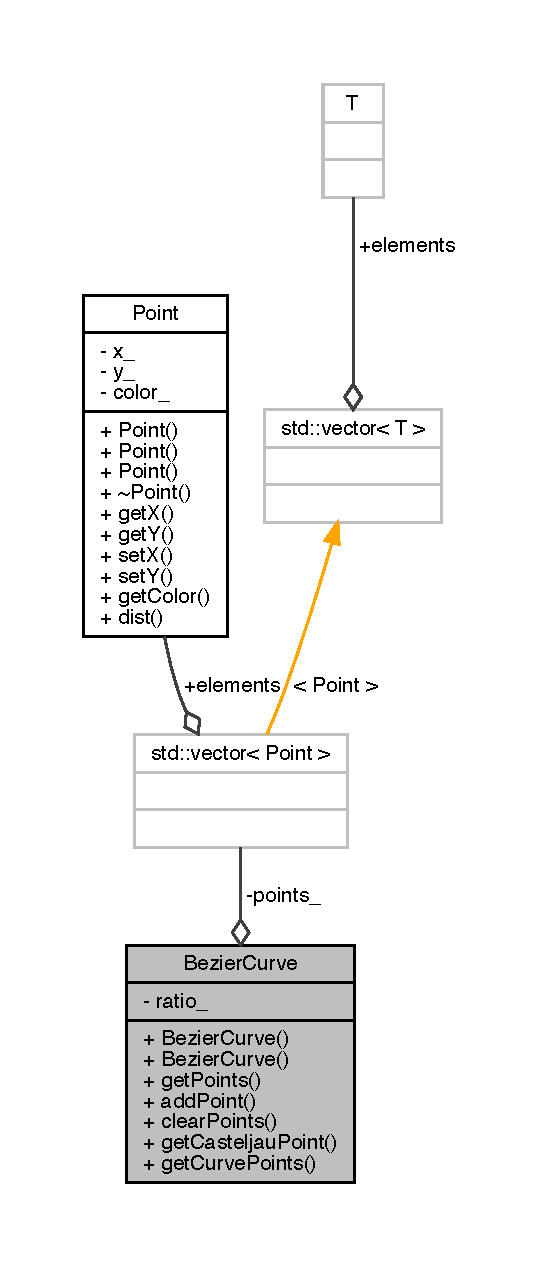
\includegraphics[height=550pt]{class_bezier_curve__coll__graph}
\end{center}
\end{figure}
\subsection*{Public Member Functions}
\begin{DoxyCompactItemize}
\item 
\mbox{\hyperlink{class_bezier_curve_af30b8df568e50499b596aff578198425}{Bezier\+Curve}} ()
\begin{DoxyCompactList}\small\item\em Default constructor. \end{DoxyCompactList}\item 
\mbox{\hyperlink{class_bezier_curve_abf9565fc1a6be43b0f1503e2db52ffd1}{Bezier\+Curve}} (std\+::vector$<$ \mbox{\hyperlink{class_point}{Point}} $>$ points)
\begin{DoxyCompactList}\small\item\em Valued constructor. \end{DoxyCompactList}\item 
std\+::vector$<$ \mbox{\hyperlink{class_point}{Point}} $>$ \mbox{\hyperlink{class_bezier_curve_a0ebb942d8285628bead89d154f39e616}{get\+Points}} () const
\begin{DoxyCompactList}\small\item\em Getter for points\+\_\+. \end{DoxyCompactList}\item 
void \mbox{\hyperlink{class_bezier_curve_a38d16c18b36ae45619b05e26e226cf34}{add\+Point}} (\mbox{\hyperlink{class_point}{Point}} P)
\begin{DoxyCompactList}\small\item\em Add a new point in the Bezier Curve. \end{DoxyCompactList}\item 
void \mbox{\hyperlink{class_bezier_curve_a0ba8ce66d5af5971ae6a1b506029728e}{clear\+Points}} ()
\begin{DoxyCompactList}\small\item\em Empty the vector points\+\_\+. \end{DoxyCompactList}\item 
\mbox{\hyperlink{class_point}{Point}} \mbox{\hyperlink{class_bezier_curve_a7e0c40cb373da6aa1aa1acd5fce9d503}{get\+Casteljau\+Point}} (int c, int index, double t)
\begin{DoxyCompactList}\small\item\em Get the point computed by De Casteljau\textquotesingle{}s algorithm. \end{DoxyCompactList}\item 
std\+::vector$<$ \mbox{\hyperlink{class_point}{Point}} $>$ \mbox{\hyperlink{class_bezier_curve_a2b4482d322a84df3fa22f4e491cb2bc3}{get\+Curve\+Points}} ()
\begin{DoxyCompactList}\small\item\em Get the vector of points to draw the Bezier curve. \end{DoxyCompactList}\end{DoxyCompactItemize}
\subsection*{Private Attributes}
\begin{DoxyCompactItemize}
\item 
std\+::vector$<$ \mbox{\hyperlink{class_point}{Point}} $>$ \mbox{\hyperlink{class_bezier_curve_a73c8f89d9002be75295e6a0546547189}{points\+\_\+}}
\item 
double \mbox{\hyperlink{class_bezier_curve_a308d7d0afc02da11ed0020508d537818}{step\+\_\+}} = 0.\+000001
\end{DoxyCompactItemize}


\subsection{Constructor \& Destructor Documentation}
\mbox{\Hypertarget{class_bezier_curve_af30b8df568e50499b596aff578198425}\label{class_bezier_curve_af30b8df568e50499b596aff578198425}} 
\index{Bezier\+Curve@{Bezier\+Curve}!Bezier\+Curve@{Bezier\+Curve}}
\index{Bezier\+Curve@{Bezier\+Curve}!Bezier\+Curve@{Bezier\+Curve}}
\subsubsection{\texorpdfstring{Bezier\+Curve()}{BezierCurve()}\hspace{0.1cm}{\footnotesize\ttfamily [1/2]}}
{\footnotesize\ttfamily Bezier\+Curve\+::\+Bezier\+Curve (\begin{DoxyParamCaption}{ }\end{DoxyParamCaption})\hspace{0.3cm}{\ttfamily [inline]}}



Default constructor. 


\begin{DoxyCode}
26 \{\};
\end{DoxyCode}
\mbox{\Hypertarget{class_bezier_curve_abf9565fc1a6be43b0f1503e2db52ffd1}\label{class_bezier_curve_abf9565fc1a6be43b0f1503e2db52ffd1}} 
\index{Bezier\+Curve@{Bezier\+Curve}!Bezier\+Curve@{Bezier\+Curve}}
\index{Bezier\+Curve@{Bezier\+Curve}!Bezier\+Curve@{Bezier\+Curve}}
\subsubsection{\texorpdfstring{Bezier\+Curve()}{BezierCurve()}\hspace{0.1cm}{\footnotesize\ttfamily [2/2]}}
{\footnotesize\ttfamily Bezier\+Curve\+::\+Bezier\+Curve (\begin{DoxyParamCaption}\item[{std\+::vector$<$ \mbox{\hyperlink{class_point}{Point}} $>$}]{points }\end{DoxyParamCaption})}



Valued constructor. 


\begin{DoxyParams}{Parameters}
{\em points} & Vector of points of the Bezier curve \\
\hline
\end{DoxyParams}

\begin{DoxyCode}
14                                                 \{
15     \mbox{\hyperlink{class_bezier_curve_a73c8f89d9002be75295e6a0546547189}{points\_}} = points;
16 \}
\end{DoxyCode}


\subsection{Member Function Documentation}
\mbox{\Hypertarget{class_bezier_curve_a38d16c18b36ae45619b05e26e226cf34}\label{class_bezier_curve_a38d16c18b36ae45619b05e26e226cf34}} 
\index{Bezier\+Curve@{Bezier\+Curve}!add\+Point@{add\+Point}}
\index{add\+Point@{add\+Point}!Bezier\+Curve@{Bezier\+Curve}}
\subsubsection{\texorpdfstring{add\+Point()}{addPoint()}}
{\footnotesize\ttfamily void Bezier\+Curve\+::add\+Point (\begin{DoxyParamCaption}\item[{\mbox{\hyperlink{class_point}{Point}}}]{P }\end{DoxyParamCaption})}



Add a new point in the Bezier Curve. 

\begin{DoxyReturn}{Returns}
The computed \mbox{\hyperlink{class_point}{Point}} 
\end{DoxyReturn}

\begin{DoxyCode}
18                                   \{
19     \mbox{\hyperlink{class_bezier_curve_a73c8f89d9002be75295e6a0546547189}{points\_}}.push\_back(P);
20 \}
\end{DoxyCode}
\mbox{\Hypertarget{class_bezier_curve_a0ba8ce66d5af5971ae6a1b506029728e}\label{class_bezier_curve_a0ba8ce66d5af5971ae6a1b506029728e}} 
\index{Bezier\+Curve@{Bezier\+Curve}!clear\+Points@{clear\+Points}}
\index{clear\+Points@{clear\+Points}!Bezier\+Curve@{Bezier\+Curve}}
\subsubsection{\texorpdfstring{clear\+Points()}{clearPoints()}}
{\footnotesize\ttfamily void Bezier\+Curve\+::clear\+Points (\begin{DoxyParamCaption}{ }\end{DoxyParamCaption})}



Empty the vector points\+\_\+. 


\begin{DoxyCode}
22                               \{
23     \mbox{\hyperlink{class_bezier_curve_a73c8f89d9002be75295e6a0546547189}{points\_}}.clear();
24 \}
\end{DoxyCode}
\mbox{\Hypertarget{class_bezier_curve_a7e0c40cb373da6aa1aa1acd5fce9d503}\label{class_bezier_curve_a7e0c40cb373da6aa1aa1acd5fce9d503}} 
\index{Bezier\+Curve@{Bezier\+Curve}!get\+Casteljau\+Point@{get\+Casteljau\+Point}}
\index{get\+Casteljau\+Point@{get\+Casteljau\+Point}!Bezier\+Curve@{Bezier\+Curve}}
\subsubsection{\texorpdfstring{get\+Casteljau\+Point()}{getCasteljauPoint()}}
{\footnotesize\ttfamily \mbox{\hyperlink{class_point}{Point}} Bezier\+Curve\+::get\+Casteljau\+Point (\begin{DoxyParamCaption}\item[{int}]{c,  }\item[{int}]{index,  }\item[{double}]{t }\end{DoxyParamCaption})}



Get the point computed by De Casteljau\textquotesingle{}s algorithm. 


\begin{DoxyParams}{Parameters}
{\em c} & The size of the current points vector \\
\hline
{\em index} & \\
\hline
{\em t} & Parameter \\
\hline
\end{DoxyParams}
\begin{DoxyReturn}{Returns}
The computed \mbox{\hyperlink{class_point}{Point}} 
\end{DoxyReturn}

\begin{DoxyCode}
26                                                                \{
27     \textcolor{keywordflow}{if} (c == 0) \{
28         \textcolor{keywordflow}{return} \mbox{\hyperlink{class_bezier_curve_a73c8f89d9002be75295e6a0546547189}{points\_}}[index];
29     \}
30     \mbox{\hyperlink{class_point}{Point}} P1 = \mbox{\hyperlink{class_bezier_curve_a7e0c40cb373da6aa1aa1acd5fce9d503}{getCasteljauPoint}}(c-1, index, t);
31     \mbox{\hyperlink{class_point}{Point}} P2 = \mbox{\hyperlink{class_bezier_curve_a7e0c40cb373da6aa1aa1acd5fce9d503}{getCasteljauPoint}}(c-1, index+1, t);
32     \textcolor{keywordflow}{return} \mbox{\hyperlink{class_point}{Point}}(round((1-t) * P1.\mbox{\hyperlink{class_point_ac9d5859db121c7d1b89ca89266dca0a3}{getX}}() + t * P2.\mbox{\hyperlink{class_point_ac9d5859db121c7d1b89ca89266dca0a3}{getX}}()), round((1-t) * P1.
      \mbox{\hyperlink{class_point_a86d10ff46e08462c45b15a8c7ef62d61}{getY}}() + t * P2.\mbox{\hyperlink{class_point_a86d10ff46e08462c45b15a8c7ef62d61}{getY}}()), \mbox{\hyperlink{class_bezier_curve_a73c8f89d9002be75295e6a0546547189}{points\_}}.begin()->getColor()[0], \mbox{\hyperlink{class_bezier_curve_a73c8f89d9002be75295e6a0546547189}{points\_}}.begin()->getColor()[
      1], \mbox{\hyperlink{class_bezier_curve_a73c8f89d9002be75295e6a0546547189}{points\_}}.begin()->getColor()[2]);
33 \}
\end{DoxyCode}
\mbox{\Hypertarget{class_bezier_curve_a2b4482d322a84df3fa22f4e491cb2bc3}\label{class_bezier_curve_a2b4482d322a84df3fa22f4e491cb2bc3}} 
\index{Bezier\+Curve@{Bezier\+Curve}!get\+Curve\+Points@{get\+Curve\+Points}}
\index{get\+Curve\+Points@{get\+Curve\+Points}!Bezier\+Curve@{Bezier\+Curve}}
\subsubsection{\texorpdfstring{get\+Curve\+Points()}{getCurvePoints()}}
{\footnotesize\ttfamily std\+::vector$<$ \mbox{\hyperlink{class_point}{Point}} $>$ Bezier\+Curve\+::get\+Curve\+Points (\begin{DoxyParamCaption}{ }\end{DoxyParamCaption})}



Get the vector of points to draw the Bezier curve. 

Compute the points for a given precision \begin{DoxyReturn}{Returns}
The vector containing the points of the curve 
\end{DoxyReturn}

\begin{DoxyCode}
35                                              \{
36     std::vector<Point> res;
37     \textcolor{keywordflow}{for} (\textcolor{keywordtype}{double} t = 0.0; t <= 1; t += \mbox{\hyperlink{class_bezier_curve_a308d7d0afc02da11ed0020508d537818}{step\_}}) \{
38         res.push\_back(\mbox{\hyperlink{class_bezier_curve_a7e0c40cb373da6aa1aa1acd5fce9d503}{getCasteljauPoint}}(\mbox{\hyperlink{class_bezier_curve_a73c8f89d9002be75295e6a0546547189}{points\_}}.size()-1, 0, t));
39     \}
40     \textcolor{keywordflow}{return} res;
41 \}
\end{DoxyCode}
\mbox{\Hypertarget{class_bezier_curve_a0ebb942d8285628bead89d154f39e616}\label{class_bezier_curve_a0ebb942d8285628bead89d154f39e616}} 
\index{Bezier\+Curve@{Bezier\+Curve}!get\+Points@{get\+Points}}
\index{get\+Points@{get\+Points}!Bezier\+Curve@{Bezier\+Curve}}
\subsubsection{\texorpdfstring{get\+Points()}{getPoints()}}
{\footnotesize\ttfamily std\+::vector$<$\mbox{\hyperlink{class_point}{Point}}$>$ Bezier\+Curve\+::get\+Points (\begin{DoxyParamCaption}{ }\end{DoxyParamCaption}) const}



Getter for points\+\_\+. 

\begin{DoxyReturn}{Returns}
points\+\_\+ 
\end{DoxyReturn}


\subsection{Member Data Documentation}
\mbox{\Hypertarget{class_bezier_curve_a73c8f89d9002be75295e6a0546547189}\label{class_bezier_curve_a73c8f89d9002be75295e6a0546547189}} 
\index{Bezier\+Curve@{Bezier\+Curve}!points\+\_\+@{points\+\_\+}}
\index{points\+\_\+@{points\+\_\+}!Bezier\+Curve@{Bezier\+Curve}}
\subsubsection{\texorpdfstring{points\+\_\+}{points\_}}
{\footnotesize\ttfamily std\+::vector$<$\mbox{\hyperlink{class_point}{Point}}$>$ Bezier\+Curve\+::points\+\_\+\hspace{0.3cm}{\ttfamily [private]}}

Control points of a Bezier curve \mbox{\Hypertarget{class_bezier_curve_a308d7d0afc02da11ed0020508d537818}\label{class_bezier_curve_a308d7d0afc02da11ed0020508d537818}} 
\index{Bezier\+Curve@{Bezier\+Curve}!step\+\_\+@{step\+\_\+}}
\index{step\+\_\+@{step\+\_\+}!Bezier\+Curve@{Bezier\+Curve}}
\subsubsection{\texorpdfstring{step\+\_\+}{step\_}}
{\footnotesize\ttfamily double Bezier\+Curve\+::step\+\_\+ = 0.\+000001\hspace{0.3cm}{\ttfamily [private]}}

Approximation error 

The documentation for this class was generated from the following files\+:\begin{DoxyCompactItemize}
\item 
/\+Users/\+Kevin\+Xu/\+Documents/\+Ecole\+\_\+\+Ingé/2\+A/\+S3/\+P\+A\+P/\+P\+A\+P\+\_\+\+Project/\+Projet/src/\mbox{\hyperlink{_bezier_curve_8h}{Bezier\+Curve.\+h}}\item 
/\+Users/\+Kevin\+Xu/\+Documents/\+Ecole\+\_\+\+Ingé/2\+A/\+S3/\+P\+A\+P/\+P\+A\+P\+\_\+\+Project/\+Projet/src/\mbox{\hyperlink{_bezier_curve_8cpp}{Bezier\+Curve.\+cpp}}\end{DoxyCompactItemize}

\hypertarget{class_font_v1}{}\section{Font\+V1 Class Reference}
\label{class_font_v1}\index{Font\+V1@{Font\+V1}}


{\ttfamily \#include $<$Font\+V1.\+h$>$}



Inheritance diagram for Font\+V1\+:\nopagebreak
\begin{figure}[H]
\begin{center}
\leavevmode
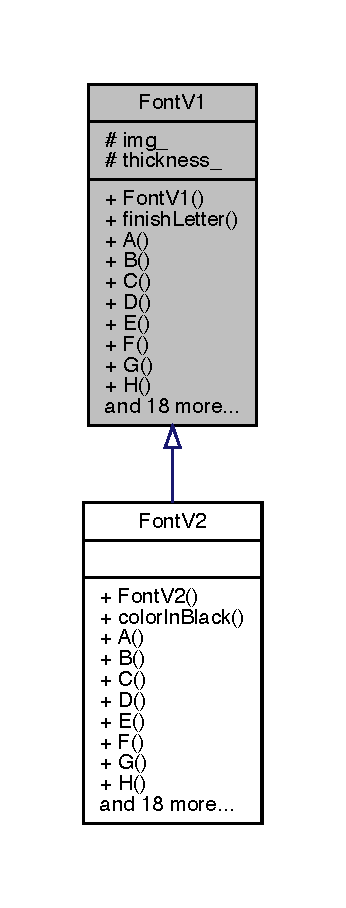
\includegraphics[height=550pt]{class_font_v1__inherit__graph}
\end{center}
\end{figure}


Collaboration diagram for Font\+V1\+:\nopagebreak
\begin{figure}[H]
\begin{center}
\leavevmode
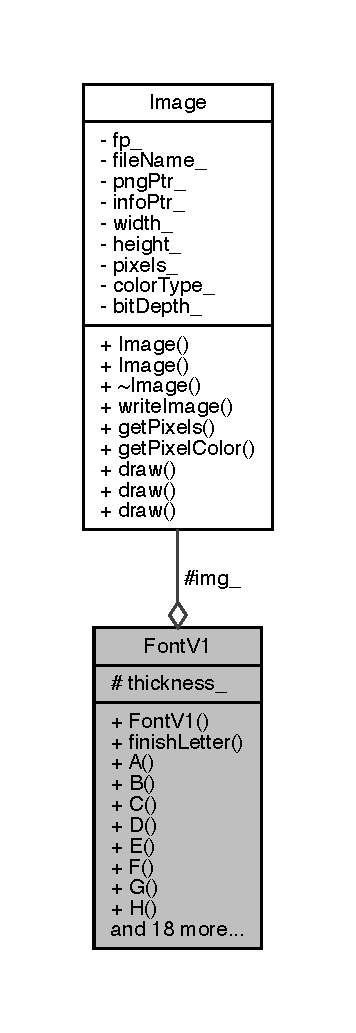
\includegraphics[width=171pt]{class_font_v1__coll__graph}
\end{center}
\end{figure}
\subsection*{Public Member Functions}
\begin{DoxyCompactItemize}
\item 
\mbox{\hyperlink{class_font_v1_ada1ed699d42679f81146af4bc20db006}{Font\+V1}} (char $\ast$image\+Name)
\begin{DoxyCompactList}\small\item\em Valued constructor. \end{DoxyCompactList}\item 
void \mbox{\hyperlink{class_font_v1_a29e1b96b06056aad8542c3d2ac79ebf2}{finish\+Letter}} ()
\begin{DoxyCompactList}\small\item\em Write the letter on the image. \end{DoxyCompactList}\item 
void \mbox{\hyperlink{class_font_v1_a29afd2079bc41cdec9d3de6bb4e1be52}{A}} ()
\begin{DoxyCompactList}\small\item\em Draw the contour of the letter A on the \mbox{\hyperlink{class_image}{Image}} img\+\_\+. \end{DoxyCompactList}\item 
void \mbox{\hyperlink{class_font_v1_a620ee7876d479807f73481f27be48f2a}{B}} ()
\begin{DoxyCompactList}\small\item\em Draw the contour of the letter B on the \mbox{\hyperlink{class_image}{Image}} img\+\_\+. \end{DoxyCompactList}\item 
void \mbox{\hyperlink{class_font_v1_a80602716ae6907fa518fbb50eeda2515}{C}} ()
\begin{DoxyCompactList}\small\item\em Draw the contour of the letter C on the \mbox{\hyperlink{class_image}{Image}} img\+\_\+. \end{DoxyCompactList}\item 
void \mbox{\hyperlink{class_font_v1_a3f4558aabfef6e0783c2294aecf215d0}{D}} ()
\begin{DoxyCompactList}\small\item\em Draw the contour of the letter D on the \mbox{\hyperlink{class_image}{Image}} img\+\_\+. \end{DoxyCompactList}\item 
void \mbox{\hyperlink{class_font_v1_ab8a34299af7a36cfd94c2691b579a0fa}{E}} ()
\begin{DoxyCompactList}\small\item\em Draw the contour of the letter E on the \mbox{\hyperlink{class_image}{Image}} img\+\_\+. \end{DoxyCompactList}\item 
void \mbox{\hyperlink{class_font_v1_a40dd925bee9092d13ba1a00546cc7160}{F}} ()
\begin{DoxyCompactList}\small\item\em Draw the contour of the letter F on the \mbox{\hyperlink{class_image}{Image}} img\+\_\+. \end{DoxyCompactList}\item 
void \mbox{\hyperlink{class_font_v1_a9806041ba05556826ba6b4a0760fcee4}{G}} ()
\begin{DoxyCompactList}\small\item\em Draw the contour of the letter G on the \mbox{\hyperlink{class_image}{Image}} img\+\_\+. \end{DoxyCompactList}\item 
void \mbox{\hyperlink{class_font_v1_aac6c3d7f8116c21fd9339d07aa63a797}{H}} ()
\begin{DoxyCompactList}\small\item\em Draw the contour of the letter H on the \mbox{\hyperlink{class_image}{Image}} img\+\_\+. \end{DoxyCompactList}\item 
void \mbox{\hyperlink{class_font_v1_aab86d5ae867a26e0384c919f82f0bcf1}{I}} ()
\begin{DoxyCompactList}\small\item\em Draw the contour of the letter I on the \mbox{\hyperlink{class_image}{Image}} img\+\_\+. \end{DoxyCompactList}\item 
void \mbox{\hyperlink{class_font_v1_a3fe315f13fd21c6dbd5f81113cd1c3f6}{J}} ()
\begin{DoxyCompactList}\small\item\em Draw the contour of the letter J on the \mbox{\hyperlink{class_image}{Image}} img\+\_\+. \end{DoxyCompactList}\item 
void \mbox{\hyperlink{class_font_v1_a45ed7d1ac12bd32f458b5b144dd132ba}{K}} ()
\begin{DoxyCompactList}\small\item\em Draw the contour of the letter K on the \mbox{\hyperlink{class_image}{Image}} img\+\_\+. \end{DoxyCompactList}\item 
void \mbox{\hyperlink{class_font_v1_a17ba426bfb42af35ea882ab3beeba734}{L}} ()
\begin{DoxyCompactList}\small\item\em Draw the contour of the letter L on the \mbox{\hyperlink{class_image}{Image}} img\+\_\+. \end{DoxyCompactList}\item 
void \mbox{\hyperlink{class_font_v1_a69afdf545ed6bccbb31efaef5d6d4219}{M}} ()
\begin{DoxyCompactList}\small\item\em Draw the contour of the letter M on the \mbox{\hyperlink{class_image}{Image}} img\+\_\+. \end{DoxyCompactList}\item 
void \mbox{\hyperlink{class_font_v1_a725c93ea00d851ca5b43c0d594f1d6d0}{N}} ()
\begin{DoxyCompactList}\small\item\em Draw the contour of the letter N on the \mbox{\hyperlink{class_image}{Image}} img\+\_\+. \end{DoxyCompactList}\item 
void \mbox{\hyperlink{class_font_v1_a9338f8d780e9913a848310355973ebf3}{O}} ()
\begin{DoxyCompactList}\small\item\em Draw the contour of the letter O on the \mbox{\hyperlink{class_image}{Image}} img\+\_\+. \end{DoxyCompactList}\item 
void \mbox{\hyperlink{class_font_v1_aeaf56ebe48a78aedf53626f50f10ee4d}{P}} ()
\begin{DoxyCompactList}\small\item\em Draw the contour of the letter P on the \mbox{\hyperlink{class_image}{Image}} img\+\_\+. \end{DoxyCompactList}\item 
void \mbox{\hyperlink{class_font_v1_af7ffd76bf02756d0d1e2d3eab4c65c40}{Q}} ()
\begin{DoxyCompactList}\small\item\em Draw the contour of the letter Q on the \mbox{\hyperlink{class_image}{Image}} img\+\_\+. \end{DoxyCompactList}\item 
void \mbox{\hyperlink{class_font_v1_ab3f9a7e62f7d08792d9028da68f5787e}{R}} ()
\begin{DoxyCompactList}\small\item\em Draw the contour of the letter R on the \mbox{\hyperlink{class_image}{Image}} img\+\_\+. \end{DoxyCompactList}\item 
void \mbox{\hyperlink{class_font_v1_ab6daa08377051d5af458003c665cfc09}{S}} ()
\begin{DoxyCompactList}\small\item\em Draw the contour of the letter S on the \mbox{\hyperlink{class_image}{Image}} img\+\_\+. \end{DoxyCompactList}\item 
void \mbox{\hyperlink{class_font_v1_ab520e2522e89b6ff20e42621080edd7d}{T}} ()
\begin{DoxyCompactList}\small\item\em Draw the contour of the letter T on the \mbox{\hyperlink{class_image}{Image}} img\+\_\+. \end{DoxyCompactList}\item 
void \mbox{\hyperlink{class_font_v1_a460d625b76b123ba4e67a21091d7dcce}{U}} ()
\begin{DoxyCompactList}\small\item\em Draw the contour of the letter U on the \mbox{\hyperlink{class_image}{Image}} img\+\_\+. \end{DoxyCompactList}\item 
void \mbox{\hyperlink{class_font_v1_aa5937063bd49c25ccd8993d375926fb7}{V}} ()
\begin{DoxyCompactList}\small\item\em Draw the contour of the letter V on the \mbox{\hyperlink{class_image}{Image}} img\+\_\+. \end{DoxyCompactList}\item 
void \mbox{\hyperlink{class_font_v1_aa4e67840b676dfffd3e03d873013174c}{W}} ()
\begin{DoxyCompactList}\small\item\em Draw the contour of the letter W on the \mbox{\hyperlink{class_image}{Image}} img\+\_\+. \end{DoxyCompactList}\item 
void \mbox{\hyperlink{class_font_v1_a8a93144edcf0f9bf1ac9017eb916ff82}{X}} ()
\begin{DoxyCompactList}\small\item\em Draw the contour of the letter X on the \mbox{\hyperlink{class_image}{Image}} img\+\_\+. \end{DoxyCompactList}\item 
void \mbox{\hyperlink{class_font_v1_a25827e105e44581040d8c17cc821e4f3}{Y}} ()
\begin{DoxyCompactList}\small\item\em Draw the contour of the letter Y on the \mbox{\hyperlink{class_image}{Image}} img\+\_\+. \end{DoxyCompactList}\item 
void \mbox{\hyperlink{class_font_v1_a10df574bc5aa14a43988d42db4e89504}{Z}} ()
\begin{DoxyCompactList}\small\item\em Draw the contour of the letter Z on the \mbox{\hyperlink{class_image}{Image}} img\+\_\+. \end{DoxyCompactList}\end{DoxyCompactItemize}
\subsection*{Protected Attributes}
\begin{DoxyCompactItemize}
\item 
\mbox{\hyperlink{class_image}{Image}} \mbox{\hyperlink{class_font_v1_a00569e3e3c4b70f437b63f396f735fb0}{img\+\_\+}}
\item 
int \mbox{\hyperlink{class_font_v1_aed8040e76be9a52833627b92f0fb4e5f}{thickness\+\_\+}} = 20
\end{DoxyCompactItemize}


\subsection{Constructor \& Destructor Documentation}
\mbox{\Hypertarget{class_font_v1_ada1ed699d42679f81146af4bc20db006}\label{class_font_v1_ada1ed699d42679f81146af4bc20db006}} 
\index{Font\+V1@{Font\+V1}!Font\+V1@{Font\+V1}}
\index{Font\+V1@{Font\+V1}!Font\+V1@{Font\+V1}}
\subsubsection{\texorpdfstring{Font\+V1()}{FontV1()}}
{\footnotesize\ttfamily Font\+V1\+::\+Font\+V1 (\begin{DoxyParamCaption}\item[{char $\ast$}]{image\+Name }\end{DoxyParamCaption})\hspace{0.3cm}{\ttfamily [inline]}}



Valued constructor. 


\begin{DoxyParams}{Parameters}
{\em image\+Name} & The name of the image \\
\hline
\end{DoxyParams}

\begin{DoxyCode}
27                                 : \mbox{\hyperlink{class_font_v1_a00569e3e3c4b70f437b63f396f735fb0}{img\_}}(imageName, 500, 500) \{
28         \};
\end{DoxyCode}


\subsection{Member Function Documentation}
\mbox{\Hypertarget{class_font_v1_a29afd2079bc41cdec9d3de6bb4e1be52}\label{class_font_v1_a29afd2079bc41cdec9d3de6bb4e1be52}} 
\index{Font\+V1@{Font\+V1}!A@{A}}
\index{A@{A}!Font\+V1@{Font\+V1}}
\subsubsection{\texorpdfstring{A()}{A()}}
{\footnotesize\ttfamily void Font\+V1\+::A (\begin{DoxyParamCaption}{ }\end{DoxyParamCaption})}



Draw the contour of the letter A on the \mbox{\hyperlink{class_image}{Image}} img\+\_\+. 


\begin{DoxyCode}
10               \{
11     \mbox{\hyperlink{class_bezier_curve}{BezierCurve}} curve1A;
12     std::vector<BezierCurve> curves;
13 
14     \textcolor{comment}{// haut}
15     curve1A.\mbox{\hyperlink{class_bezier_curve_a38d16c18b36ae45619b05e26e226cf34}{addPoint}}(\mbox{\hyperlink{class_point}{Point}}(240, 350));
16     curve1A.\mbox{\hyperlink{class_bezier_curve_a38d16c18b36ae45619b05e26e226cf34}{addPoint}}(\mbox{\hyperlink{class_point}{Point}}(240+\mbox{\hyperlink{class_font_v1_aed8040e76be9a52833627b92f0fb4e5f}{thickness\_}}, 350));
17     curves.push\_back(curve1A);
18 
19     \textcolor{comment}{// gauche}
20     curve1A.\mbox{\hyperlink{class_bezier_curve_a0ba8ce66d5af5971ae6a1b506029728e}{clearPoints}}();
21     curve1A.\mbox{\hyperlink{class_bezier_curve_a38d16c18b36ae45619b05e26e226cf34}{addPoint}}(\mbox{\hyperlink{class_point}{Point}}(240, 350));
22     curve1A.\mbox{\hyperlink{class_bezier_curve_a38d16c18b36ae45619b05e26e226cf34}{addPoint}}(\mbox{\hyperlink{class_point}{Point}}(150+10, 150));
23     curves.push\_back(curve1A);
24 
25     \textcolor{comment}{// droite}
26     curve1A.\mbox{\hyperlink{class_bezier_curve_a0ba8ce66d5af5971ae6a1b506029728e}{clearPoints}}();
27     curve1A.\mbox{\hyperlink{class_bezier_curve_a38d16c18b36ae45619b05e26e226cf34}{addPoint}}(\mbox{\hyperlink{class_point}{Point}}(260, 350));
28     curve1A.\mbox{\hyperlink{class_bezier_curve_a38d16c18b36ae45619b05e26e226cf34}{addPoint}}(\mbox{\hyperlink{class_point}{Point}}(350-10, 150));
29     curves.push\_back(curve1A);
30 
31     \textcolor{comment}{//bas gauche}
32     curve1A.\mbox{\hyperlink{class_bezier_curve_a0ba8ce66d5af5971ae6a1b506029728e}{clearPoints}}();
33     curve1A.\mbox{\hyperlink{class_bezier_curve_a38d16c18b36ae45619b05e26e226cf34}{addPoint}}(\mbox{\hyperlink{class_point}{Point}}(150+10, 150));
34     curve1A.\mbox{\hyperlink{class_bezier_curve_a38d16c18b36ae45619b05e26e226cf34}{addPoint}}(\mbox{\hyperlink{class_point}{Point}}(150+\mbox{\hyperlink{class_font_v1_aed8040e76be9a52833627b92f0fb4e5f}{thickness\_}}+10, 150));
35     curves.push\_back(curve1A);
36 
37     \textcolor{comment}{//bas droite}
38     curve1A.\mbox{\hyperlink{class_bezier_curve_a0ba8ce66d5af5971ae6a1b506029728e}{clearPoints}}();
39     curve1A.\mbox{\hyperlink{class_bezier_curve_a38d16c18b36ae45619b05e26e226cf34}{addPoint}}(\mbox{\hyperlink{class_point}{Point}}(350-\mbox{\hyperlink{class_font_v1_aed8040e76be9a52833627b92f0fb4e5f}{thickness\_}}-10, 150));
40     curve1A.\mbox{\hyperlink{class_bezier_curve_a38d16c18b36ae45619b05e26e226cf34}{addPoint}}(\mbox{\hyperlink{class_point}{Point}}(350-10, 150));
41     curves.push\_back(curve1A);
42 
43     \textcolor{comment}{//bas}
44     curve1A.\mbox{\hyperlink{class_bezier_curve_a0ba8ce66d5af5971ae6a1b506029728e}{clearPoints}}();
45     curve1A.\mbox{\hyperlink{class_bezier_curve_a38d16c18b36ae45619b05e26e226cf34}{addPoint}}(\mbox{\hyperlink{class_point}{Point}}(150+\mbox{\hyperlink{class_font_v1_aed8040e76be9a52833627b92f0fb4e5f}{thickness\_}}+10, 150));
46     curve1A.\mbox{\hyperlink{class_bezier_curve_a38d16c18b36ae45619b05e26e226cf34}{addPoint}}(\mbox{\hyperlink{class_point}{Point}}(200+10, 225));
47     curves.push\_back(curve1A);
48 
49     curve1A.\mbox{\hyperlink{class_bezier_curve_a0ba8ce66d5af5971ae6a1b506029728e}{clearPoints}}();
50     curve1A.\mbox{\hyperlink{class_bezier_curve_a38d16c18b36ae45619b05e26e226cf34}{addPoint}}(\mbox{\hyperlink{class_point}{Point}}(350-\mbox{\hyperlink{class_font_v1_aed8040e76be9a52833627b92f0fb4e5f}{thickness\_}}-10, 150));
51     curve1A.\mbox{\hyperlink{class_bezier_curve_a38d16c18b36ae45619b05e26e226cf34}{addPoint}}(\mbox{\hyperlink{class_point}{Point}}(300-10, 225));
52     curves.push\_back(curve1A);
53 
54     curve1A.\mbox{\hyperlink{class_bezier_curve_a0ba8ce66d5af5971ae6a1b506029728e}{clearPoints}}();
55     curve1A.\mbox{\hyperlink{class_bezier_curve_a38d16c18b36ae45619b05e26e226cf34}{addPoint}}(\mbox{\hyperlink{class_point}{Point}}(200+10, 225));
56     curve1A.\mbox{\hyperlink{class_bezier_curve_a38d16c18b36ae45619b05e26e226cf34}{addPoint}}(\mbox{\hyperlink{class_point}{Point}}(300-10, 225));
57     curves.push\_back(curve1A);
58 
59     \textcolor{comment}{// small}
60     \textcolor{comment}{// gauche}
61     curve1A.\mbox{\hyperlink{class_bezier_curve_a0ba8ce66d5af5971ae6a1b506029728e}{clearPoints}}();
62     curve1A.\mbox{\hyperlink{class_bezier_curve_a38d16c18b36ae45619b05e26e226cf34}{addPoint}}(\mbox{\hyperlink{class_point}{Point}}(250, 350-\mbox{\hyperlink{class_font_v1_aed8040e76be9a52833627b92f0fb4e5f}{thickness\_}}));
63     curve1A.\mbox{\hyperlink{class_bezier_curve_a38d16c18b36ae45619b05e26e226cf34}{addPoint}}(\mbox{\hyperlink{class_point}{Point}}(200+0.5*\mbox{\hyperlink{class_font_v1_aed8040e76be9a52833627b92f0fb4e5f}{thickness\_}}+10, 225+
      \mbox{\hyperlink{class_font_v1_aed8040e76be9a52833627b92f0fb4e5f}{thickness\_}}));
64     curves.push\_back(curve1A);
65 
66     \textcolor{comment}{// droite}
67     curve1A.\mbox{\hyperlink{class_bezier_curve_a0ba8ce66d5af5971ae6a1b506029728e}{clearPoints}}();
68     curve1A.\mbox{\hyperlink{class_bezier_curve_a38d16c18b36ae45619b05e26e226cf34}{addPoint}}(\mbox{\hyperlink{class_point}{Point}}(250, 350-\mbox{\hyperlink{class_font_v1_aed8040e76be9a52833627b92f0fb4e5f}{thickness\_}}));
69     curve1A.\mbox{\hyperlink{class_bezier_curve_a38d16c18b36ae45619b05e26e226cf34}{addPoint}}(\mbox{\hyperlink{class_point}{Point}}(300-0.5*\mbox{\hyperlink{class_font_v1_aed8040e76be9a52833627b92f0fb4e5f}{thickness\_}}-10, 225+
      \mbox{\hyperlink{class_font_v1_aed8040e76be9a52833627b92f0fb4e5f}{thickness\_}}));
70     curves.push\_back(curve1A);
71 
72     \textcolor{comment}{// bas}
73     curve1A.\mbox{\hyperlink{class_bezier_curve_a0ba8ce66d5af5971ae6a1b506029728e}{clearPoints}}();
74     curve1A.\mbox{\hyperlink{class_bezier_curve_a38d16c18b36ae45619b05e26e226cf34}{addPoint}}(\mbox{\hyperlink{class_point}{Point}}(200+0.5*\mbox{\hyperlink{class_font_v1_aed8040e76be9a52833627b92f0fb4e5f}{thickness\_}}+10, 225+
      \mbox{\hyperlink{class_font_v1_aed8040e76be9a52833627b92f0fb4e5f}{thickness\_}}));
75     curve1A.\mbox{\hyperlink{class_bezier_curve_a38d16c18b36ae45619b05e26e226cf34}{addPoint}}(\mbox{\hyperlink{class_point}{Point}}(300-0.5*\mbox{\hyperlink{class_font_v1_aed8040e76be9a52833627b92f0fb4e5f}{thickness\_}}-10, 225+
      \mbox{\hyperlink{class_font_v1_aed8040e76be9a52833627b92f0fb4e5f}{thickness\_}}));
76     curves.push\_back(curve1A);
77 
78     \mbox{\hyperlink{class_font_v1_a00569e3e3c4b70f437b63f396f735fb0}{img\_}}.\mbox{\hyperlink{class_image_a8d162f3cab956131d58708c09aa560b0}{draw}}(curves);
79 \}
\end{DoxyCode}
\mbox{\Hypertarget{class_font_v1_a620ee7876d479807f73481f27be48f2a}\label{class_font_v1_a620ee7876d479807f73481f27be48f2a}} 
\index{Font\+V1@{Font\+V1}!B@{B}}
\index{B@{B}!Font\+V1@{Font\+V1}}
\subsubsection{\texorpdfstring{B()}{B()}}
{\footnotesize\ttfamily void Font\+V1\+::B (\begin{DoxyParamCaption}{ }\end{DoxyParamCaption})}



Draw the contour of the letter B on the \mbox{\hyperlink{class_image}{Image}} img\+\_\+. 


\begin{DoxyCode}
81               \{
82     \mbox{\hyperlink{class_bezier_curve}{BezierCurve}} curve1B;
83     std::vector<BezierCurve> curves;
84 
85     \textcolor{comment}{// gauche}
86     curve1B.\mbox{\hyperlink{class_bezier_curve_a0ba8ce66d5af5971ae6a1b506029728e}{clearPoints}}();
87     curve1B.\mbox{\hyperlink{class_bezier_curve_a38d16c18b36ae45619b05e26e226cf34}{addPoint}}(\mbox{\hyperlink{class_point}{Point}}(150, 350));
88     curve1B.\mbox{\hyperlink{class_bezier_curve_a38d16c18b36ae45619b05e26e226cf34}{addPoint}}(\mbox{\hyperlink{class_point}{Point}}(150, 150));
89     curves.push\_back(curve1B);
90 
91     \textcolor{comment}{// haut}
92     curve1B.\mbox{\hyperlink{class_bezier_curve_a0ba8ce66d5af5971ae6a1b506029728e}{clearPoints}}();
93     curve1B.\mbox{\hyperlink{class_bezier_curve_a38d16c18b36ae45619b05e26e226cf34}{addPoint}}(\mbox{\hyperlink{class_point}{Point}}(250, 350));
94     curve1B.\mbox{\hyperlink{class_bezier_curve_a38d16c18b36ae45619b05e26e226cf34}{addPoint}}(\mbox{\hyperlink{class_point}{Point}}(150, 350));
95     curves.push\_back(curve1B);
96 
97     \textcolor{comment}{// bas}
98     curve1B.\mbox{\hyperlink{class_bezier_curve_a0ba8ce66d5af5971ae6a1b506029728e}{clearPoints}}();
99     curve1B.\mbox{\hyperlink{class_bezier_curve_a38d16c18b36ae45619b05e26e226cf34}{addPoint}}(\mbox{\hyperlink{class_point}{Point}}(250, 150));
100     curve1B.\mbox{\hyperlink{class_bezier_curve_a38d16c18b36ae45619b05e26e226cf34}{addPoint}}(\mbox{\hyperlink{class_point}{Point}}(150, 150));
101     curves.push\_back(curve1B);
102 
103     \textcolor{comment}{// haut droite}
104     curve1B.\mbox{\hyperlink{class_bezier_curve_a0ba8ce66d5af5971ae6a1b506029728e}{clearPoints}}();
105     curve1B.\mbox{\hyperlink{class_bezier_curve_a38d16c18b36ae45619b05e26e226cf34}{addPoint}}(\mbox{\hyperlink{class_point}{Point}}(250, 350));
106     curve1B.\mbox{\hyperlink{class_bezier_curve_a38d16c18b36ae45619b05e26e226cf34}{addPoint}}(\mbox{\hyperlink{class_point}{Point}}(300, 350));
107     curve1B.\mbox{\hyperlink{class_bezier_curve_a38d16c18b36ae45619b05e26e226cf34}{addPoint}}(\mbox{\hyperlink{class_point}{Point}}(300, 300));
108     curves.push\_back(curve1B);
109 
110     curve1B.\mbox{\hyperlink{class_bezier_curve_a0ba8ce66d5af5971ae6a1b506029728e}{clearPoints}}();
111     curve1B.\mbox{\hyperlink{class_bezier_curve_a38d16c18b36ae45619b05e26e226cf34}{addPoint}}(\mbox{\hyperlink{class_point}{Point}}(250, 250));
112     curve1B.\mbox{\hyperlink{class_bezier_curve_a38d16c18b36ae45619b05e26e226cf34}{addPoint}}(\mbox{\hyperlink{class_point}{Point}}(300, 250));
113     curve1B.\mbox{\hyperlink{class_bezier_curve_a38d16c18b36ae45619b05e26e226cf34}{addPoint}}(\mbox{\hyperlink{class_point}{Point}}(300, 300));
114     curves.push\_back(curve1B);
115 
116     \textcolor{comment}{// bas droite}
117     curve1B.\mbox{\hyperlink{class_bezier_curve_a0ba8ce66d5af5971ae6a1b506029728e}{clearPoints}}();
118     curve1B.\mbox{\hyperlink{class_bezier_curve_a38d16c18b36ae45619b05e26e226cf34}{addPoint}}(\mbox{\hyperlink{class_point}{Point}}(250, 250));
119     curve1B.\mbox{\hyperlink{class_bezier_curve_a38d16c18b36ae45619b05e26e226cf34}{addPoint}}(\mbox{\hyperlink{class_point}{Point}}(300, 250));
120     curve1B.\mbox{\hyperlink{class_bezier_curve_a38d16c18b36ae45619b05e26e226cf34}{addPoint}}(\mbox{\hyperlink{class_point}{Point}}(300, 200));
121     curves.push\_back(curve1B);
122 
123     curve1B.\mbox{\hyperlink{class_bezier_curve_a0ba8ce66d5af5971ae6a1b506029728e}{clearPoints}}();
124     curve1B.\mbox{\hyperlink{class_bezier_curve_a38d16c18b36ae45619b05e26e226cf34}{addPoint}}(\mbox{\hyperlink{class_point}{Point}}(250, 150));
125     curve1B.\mbox{\hyperlink{class_bezier_curve_a38d16c18b36ae45619b05e26e226cf34}{addPoint}}(\mbox{\hyperlink{class_point}{Point}}(300, 150));
126     curve1B.\mbox{\hyperlink{class_bezier_curve_a38d16c18b36ae45619b05e26e226cf34}{addPoint}}(\mbox{\hyperlink{class_point}{Point}}(300, 200));
127     curves.push\_back(curve1B);
128 
129     \textcolor{comment}{// small }
130     \textcolor{comment}{// small haut}
131     \textcolor{comment}{// gauche}
132     curve1B.\mbox{\hyperlink{class_bezier_curve_a0ba8ce66d5af5971ae6a1b506029728e}{clearPoints}}();
133     curve1B.\mbox{\hyperlink{class_bezier_curve_a38d16c18b36ae45619b05e26e226cf34}{addPoint}}(\mbox{\hyperlink{class_point}{Point}}(150+\mbox{\hyperlink{class_font_v1_aed8040e76be9a52833627b92f0fb4e5f}{thickness\_}}, 350-\mbox{\hyperlink{class_font_v1_aed8040e76be9a52833627b92f0fb4e5f}{thickness\_}}));
134     curve1B.\mbox{\hyperlink{class_bezier_curve_a38d16c18b36ae45619b05e26e226cf34}{addPoint}}(\mbox{\hyperlink{class_point}{Point}}(150+\mbox{\hyperlink{class_font_v1_aed8040e76be9a52833627b92f0fb4e5f}{thickness\_}}, 250+0.5*
      \mbox{\hyperlink{class_font_v1_aed8040e76be9a52833627b92f0fb4e5f}{thickness\_}}));
135     curves.push\_back(curve1B);
136 
137     \textcolor{comment}{// haut}
138     curve1B.\mbox{\hyperlink{class_bezier_curve_a0ba8ce66d5af5971ae6a1b506029728e}{clearPoints}}();
139     curve1B.\mbox{\hyperlink{class_bezier_curve_a38d16c18b36ae45619b05e26e226cf34}{addPoint}}(\mbox{\hyperlink{class_point}{Point}}(250, 350-\mbox{\hyperlink{class_font_v1_aed8040e76be9a52833627b92f0fb4e5f}{thickness\_}}));
140     curve1B.\mbox{\hyperlink{class_bezier_curve_a38d16c18b36ae45619b05e26e226cf34}{addPoint}}(\mbox{\hyperlink{class_point}{Point}}(150+\mbox{\hyperlink{class_font_v1_aed8040e76be9a52833627b92f0fb4e5f}{thickness\_}}, 350-\mbox{\hyperlink{class_font_v1_aed8040e76be9a52833627b92f0fb4e5f}{thickness\_}}));
141     curves.push\_back(curve1B);
142 
143     \textcolor{comment}{// bas}
144     curve1B.\mbox{\hyperlink{class_bezier_curve_a0ba8ce66d5af5971ae6a1b506029728e}{clearPoints}}();
145     curve1B.\mbox{\hyperlink{class_bezier_curve_a38d16c18b36ae45619b05e26e226cf34}{addPoint}}(\mbox{\hyperlink{class_point}{Point}}(250, 250+0.5*\mbox{\hyperlink{class_font_v1_aed8040e76be9a52833627b92f0fb4e5f}{thickness\_}}));
146     curve1B.\mbox{\hyperlink{class_bezier_curve_a38d16c18b36ae45619b05e26e226cf34}{addPoint}}(\mbox{\hyperlink{class_point}{Point}}(150+\mbox{\hyperlink{class_font_v1_aed8040e76be9a52833627b92f0fb4e5f}{thickness\_}}, 250+0.5*
      \mbox{\hyperlink{class_font_v1_aed8040e76be9a52833627b92f0fb4e5f}{thickness\_}}));
147     curves.push\_back(curve1B);
148 
149     \textcolor{comment}{// haut droite}
150     curve1B.\mbox{\hyperlink{class_bezier_curve_a0ba8ce66d5af5971ae6a1b506029728e}{clearPoints}}();
151     curve1B.\mbox{\hyperlink{class_bezier_curve_a38d16c18b36ae45619b05e26e226cf34}{addPoint}}(\mbox{\hyperlink{class_point}{Point}}(250, 350-\mbox{\hyperlink{class_font_v1_aed8040e76be9a52833627b92f0fb4e5f}{thickness\_}}));
152     curve1B.\mbox{\hyperlink{class_bezier_curve_a38d16c18b36ae45619b05e26e226cf34}{addPoint}}(\mbox{\hyperlink{class_point}{Point}}(300-\mbox{\hyperlink{class_font_v1_aed8040e76be9a52833627b92f0fb4e5f}{thickness\_}}, 350-\mbox{\hyperlink{class_font_v1_aed8040e76be9a52833627b92f0fb4e5f}{thickness\_}}));
153     curve1B.\mbox{\hyperlink{class_bezier_curve_a38d16c18b36ae45619b05e26e226cf34}{addPoint}}(\mbox{\hyperlink{class_point}{Point}}(300-\mbox{\hyperlink{class_font_v1_aed8040e76be9a52833627b92f0fb4e5f}{thickness\_}}, 300));
154     curves.push\_back(curve1B);
155 
156     \textcolor{comment}{// bas droite}
157     curve1B.\mbox{\hyperlink{class_bezier_curve_a0ba8ce66d5af5971ae6a1b506029728e}{clearPoints}}();
158     curve1B.\mbox{\hyperlink{class_bezier_curve_a38d16c18b36ae45619b05e26e226cf34}{addPoint}}(\mbox{\hyperlink{class_point}{Point}}(300-\mbox{\hyperlink{class_font_v1_aed8040e76be9a52833627b92f0fb4e5f}{thickness\_}}, 300));
159     curve1B.\mbox{\hyperlink{class_bezier_curve_a38d16c18b36ae45619b05e26e226cf34}{addPoint}}(\mbox{\hyperlink{class_point}{Point}}(300-\mbox{\hyperlink{class_font_v1_aed8040e76be9a52833627b92f0fb4e5f}{thickness\_}}, 250+\mbox{\hyperlink{class_font_v1_aed8040e76be9a52833627b92f0fb4e5f}{thickness\_}}));
160     curve1B.\mbox{\hyperlink{class_bezier_curve_a38d16c18b36ae45619b05e26e226cf34}{addPoint}}(\mbox{\hyperlink{class_point}{Point}}(250, 250+0.5*\mbox{\hyperlink{class_font_v1_aed8040e76be9a52833627b92f0fb4e5f}{thickness\_}}));
161     curves.push\_back(curve1B);
162 
163     \textcolor{comment}{// small bas}
164     \textcolor{comment}{// gauche}
165     curve1B.\mbox{\hyperlink{class_bezier_curve_a0ba8ce66d5af5971ae6a1b506029728e}{clearPoints}}();
166     curve1B.\mbox{\hyperlink{class_bezier_curve_a38d16c18b36ae45619b05e26e226cf34}{addPoint}}(\mbox{\hyperlink{class_point}{Point}}(150+\mbox{\hyperlink{class_font_v1_aed8040e76be9a52833627b92f0fb4e5f}{thickness\_}}, 150+\mbox{\hyperlink{class_font_v1_aed8040e76be9a52833627b92f0fb4e5f}{thickness\_}}));
167     curve1B.\mbox{\hyperlink{class_bezier_curve_a38d16c18b36ae45619b05e26e226cf34}{addPoint}}(\mbox{\hyperlink{class_point}{Point}}(150+\mbox{\hyperlink{class_font_v1_aed8040e76be9a52833627b92f0fb4e5f}{thickness\_}}, 250-0.5*
      \mbox{\hyperlink{class_font_v1_aed8040e76be9a52833627b92f0fb4e5f}{thickness\_}}));
168     curves.push\_back(curve1B);
169 
170     \textcolor{comment}{// haut}
171     curve1B.\mbox{\hyperlink{class_bezier_curve_a0ba8ce66d5af5971ae6a1b506029728e}{clearPoints}}();
172     curve1B.\mbox{\hyperlink{class_bezier_curve_a38d16c18b36ae45619b05e26e226cf34}{addPoint}}(\mbox{\hyperlink{class_point}{Point}}(250, 250-0.5*\mbox{\hyperlink{class_font_v1_aed8040e76be9a52833627b92f0fb4e5f}{thickness\_}}));
173     curve1B.\mbox{\hyperlink{class_bezier_curve_a38d16c18b36ae45619b05e26e226cf34}{addPoint}}(\mbox{\hyperlink{class_point}{Point}}(150+\mbox{\hyperlink{class_font_v1_aed8040e76be9a52833627b92f0fb4e5f}{thickness\_}}, 250-0.5*
      \mbox{\hyperlink{class_font_v1_aed8040e76be9a52833627b92f0fb4e5f}{thickness\_}}));
174     curves.push\_back(curve1B);
175 
176     \textcolor{comment}{// bas}
177     curve1B.\mbox{\hyperlink{class_bezier_curve_a0ba8ce66d5af5971ae6a1b506029728e}{clearPoints}}();
178     curve1B.\mbox{\hyperlink{class_bezier_curve_a38d16c18b36ae45619b05e26e226cf34}{addPoint}}(\mbox{\hyperlink{class_point}{Point}}(150+\mbox{\hyperlink{class_font_v1_aed8040e76be9a52833627b92f0fb4e5f}{thickness\_}}, 150+\mbox{\hyperlink{class_font_v1_aed8040e76be9a52833627b92f0fb4e5f}{thickness\_}}));
179     curve1B.\mbox{\hyperlink{class_bezier_curve_a38d16c18b36ae45619b05e26e226cf34}{addPoint}}(\mbox{\hyperlink{class_point}{Point}}(250, 150+\mbox{\hyperlink{class_font_v1_aed8040e76be9a52833627b92f0fb4e5f}{thickness\_}}));
180     curves.push\_back(curve1B);
181 
182     \textcolor{comment}{// haut droite}
183     curve1B.\mbox{\hyperlink{class_bezier_curve_a0ba8ce66d5af5971ae6a1b506029728e}{clearPoints}}();
184     curve1B.\mbox{\hyperlink{class_bezier_curve_a38d16c18b36ae45619b05e26e226cf34}{addPoint}}(\mbox{\hyperlink{class_point}{Point}}(250, 250-0.5*\mbox{\hyperlink{class_font_v1_aed8040e76be9a52833627b92f0fb4e5f}{thickness\_}}));
185     curve1B.\mbox{\hyperlink{class_bezier_curve_a38d16c18b36ae45619b05e26e226cf34}{addPoint}}(\mbox{\hyperlink{class_point}{Point}}(300-\mbox{\hyperlink{class_font_v1_aed8040e76be9a52833627b92f0fb4e5f}{thickness\_}}, 250-\mbox{\hyperlink{class_font_v1_aed8040e76be9a52833627b92f0fb4e5f}{thickness\_}}));
186     curve1B.\mbox{\hyperlink{class_bezier_curve_a38d16c18b36ae45619b05e26e226cf34}{addPoint}}(\mbox{\hyperlink{class_point}{Point}}(300-\mbox{\hyperlink{class_font_v1_aed8040e76be9a52833627b92f0fb4e5f}{thickness\_}}, 200));
187     curves.push\_back(curve1B);
188 
189     \textcolor{comment}{// bas droite}
190     curve1B.\mbox{\hyperlink{class_bezier_curve_a0ba8ce66d5af5971ae6a1b506029728e}{clearPoints}}();
191     curve1B.\mbox{\hyperlink{class_bezier_curve_a38d16c18b36ae45619b05e26e226cf34}{addPoint}}(\mbox{\hyperlink{class_point}{Point}}(300-\mbox{\hyperlink{class_font_v1_aed8040e76be9a52833627b92f0fb4e5f}{thickness\_}}, 200));
192     curve1B.\mbox{\hyperlink{class_bezier_curve_a38d16c18b36ae45619b05e26e226cf34}{addPoint}}(\mbox{\hyperlink{class_point}{Point}}(300-\mbox{\hyperlink{class_font_v1_aed8040e76be9a52833627b92f0fb4e5f}{thickness\_}}, 150+\mbox{\hyperlink{class_font_v1_aed8040e76be9a52833627b92f0fb4e5f}{thickness\_}}));
193     curve1B.\mbox{\hyperlink{class_bezier_curve_a38d16c18b36ae45619b05e26e226cf34}{addPoint}}(\mbox{\hyperlink{class_point}{Point}}(250, 150+\mbox{\hyperlink{class_font_v1_aed8040e76be9a52833627b92f0fb4e5f}{thickness\_}}));
194     curves.push\_back(curve1B);
195 
196     \mbox{\hyperlink{class_font_v1_a00569e3e3c4b70f437b63f396f735fb0}{img\_}}.\mbox{\hyperlink{class_image_a8d162f3cab956131d58708c09aa560b0}{draw}}(curves);
197 \}
\end{DoxyCode}
\mbox{\Hypertarget{class_font_v1_a80602716ae6907fa518fbb50eeda2515}\label{class_font_v1_a80602716ae6907fa518fbb50eeda2515}} 
\index{Font\+V1@{Font\+V1}!C@{C}}
\index{C@{C}!Font\+V1@{Font\+V1}}
\subsubsection{\texorpdfstring{C()}{C()}}
{\footnotesize\ttfamily void Font\+V1\+::C (\begin{DoxyParamCaption}{ }\end{DoxyParamCaption})}



Draw the contour of the letter C on the \mbox{\hyperlink{class_image}{Image}} img\+\_\+. 


\begin{DoxyCode}
199                \{
200     \mbox{\hyperlink{class_bezier_curve}{BezierCurve}} curve1C;
201     std::vector<BezierCurve> curves;
202 
203     \textcolor{comment}{// haut petit trait}
204     curve1C.\mbox{\hyperlink{class_bezier_curve_a0ba8ce66d5af5971ae6a1b506029728e}{clearPoints}}();
205     curve1C.\mbox{\hyperlink{class_bezier_curve_a38d16c18b36ae45619b05e26e226cf34}{addPoint}}(\mbox{\hyperlink{class_point}{Point}}(320, 320));
206     curve1C.\mbox{\hyperlink{class_bezier_curve_a38d16c18b36ae45619b05e26e226cf34}{addPoint}}(\mbox{\hyperlink{class_point}{Point}}(320-\mbox{\hyperlink{class_font_v1_aed8040e76be9a52833627b92f0fb4e5f}{thickness\_}}+3, 320-
      \mbox{\hyperlink{class_font_v1_aed8040e76be9a52833627b92f0fb4e5f}{thickness\_}}+10));
207     curves.push\_back(curve1C);
208     
209     \textcolor{comment}{// haut droite}
210     curve1C.\mbox{\hyperlink{class_bezier_curve_a0ba8ce66d5af5971ae6a1b506029728e}{clearPoints}}();
211     curve1C.\mbox{\hyperlink{class_bezier_curve_a38d16c18b36ae45619b05e26e226cf34}{addPoint}}(\mbox{\hyperlink{class_point}{Point}}(320, 320));
212     curve1C.\mbox{\hyperlink{class_bezier_curve_a38d16c18b36ae45619b05e26e226cf34}{addPoint}}(\mbox{\hyperlink{class_point}{Point}}(300, 350));
213     curve1C.\mbox{\hyperlink{class_bezier_curve_a38d16c18b36ae45619b05e26e226cf34}{addPoint}}(\mbox{\hyperlink{class_point}{Point}}(250, 350));
214     curves.push\_back(curve1C);
215 
216     \textcolor{comment}{// haut gauche}
217     curve1C.\mbox{\hyperlink{class_bezier_curve_a0ba8ce66d5af5971ae6a1b506029728e}{clearPoints}}();
218     curve1C.\mbox{\hyperlink{class_bezier_curve_a38d16c18b36ae45619b05e26e226cf34}{addPoint}}(\mbox{\hyperlink{class_point}{Point}}(170, 250));
219     curve1C.\mbox{\hyperlink{class_bezier_curve_a38d16c18b36ae45619b05e26e226cf34}{addPoint}}(\mbox{\hyperlink{class_point}{Point}}(170, 350));
220     curve1C.\mbox{\hyperlink{class_bezier_curve_a38d16c18b36ae45619b05e26e226cf34}{addPoint}}(\mbox{\hyperlink{class_point}{Point}}(250, 350));
221     curves.push\_back(curve1C);
222 
223     \textcolor{comment}{// bas gauche}
224     curve1C.\mbox{\hyperlink{class_bezier_curve_a0ba8ce66d5af5971ae6a1b506029728e}{clearPoints}}();
225     curve1C.\mbox{\hyperlink{class_bezier_curve_a38d16c18b36ae45619b05e26e226cf34}{addPoint}}(\mbox{\hyperlink{class_point}{Point}}(170, 250));
226     curve1C.\mbox{\hyperlink{class_bezier_curve_a38d16c18b36ae45619b05e26e226cf34}{addPoint}}(\mbox{\hyperlink{class_point}{Point}}(170, 150));
227     curve1C.\mbox{\hyperlink{class_bezier_curve_a38d16c18b36ae45619b05e26e226cf34}{addPoint}}(\mbox{\hyperlink{class_point}{Point}}(250, 150));
228     curves.push\_back(curve1C);
229 
230     \textcolor{comment}{// bas droite}
231     curve1C.\mbox{\hyperlink{class_bezier_curve_a0ba8ce66d5af5971ae6a1b506029728e}{clearPoints}}();
232     curve1C.\mbox{\hyperlink{class_bezier_curve_a38d16c18b36ae45619b05e26e226cf34}{addPoint}}(\mbox{\hyperlink{class_point}{Point}}(320, 320-(320-250)*2));
233     curve1C.\mbox{\hyperlink{class_bezier_curve_a38d16c18b36ae45619b05e26e226cf34}{addPoint}}(\mbox{\hyperlink{class_point}{Point}}(300, 350-(350-250)*2));
234     curve1C.\mbox{\hyperlink{class_bezier_curve_a38d16c18b36ae45619b05e26e226cf34}{addPoint}}(\mbox{\hyperlink{class_point}{Point}}(250, 350-(350-250)*2));
235     curves.push\_back(curve1C);
236 
237     \textcolor{comment}{// Small}
238     \textcolor{comment}{// haut droite}
239     curve1C.\mbox{\hyperlink{class_bezier_curve_a0ba8ce66d5af5971ae6a1b506029728e}{clearPoints}}();
240     curve1C.\mbox{\hyperlink{class_bezier_curve_a38d16c18b36ae45619b05e26e226cf34}{addPoint}}(\mbox{\hyperlink{class_point}{Point}}(320-\mbox{\hyperlink{class_font_v1_aed8040e76be9a52833627b92f0fb4e5f}{thickness\_}}+3, 320-
      \mbox{\hyperlink{class_font_v1_aed8040e76be9a52833627b92f0fb4e5f}{thickness\_}}+10));
241     curve1C.\mbox{\hyperlink{class_bezier_curve_a38d16c18b36ae45619b05e26e226cf34}{addPoint}}(\mbox{\hyperlink{class_point}{Point}}(300-\mbox{\hyperlink{class_font_v1_aed8040e76be9a52833627b92f0fb4e5f}{thickness\_}}, 350-\mbox{\hyperlink{class_font_v1_aed8040e76be9a52833627b92f0fb4e5f}{thickness\_}}));
242     curve1C.\mbox{\hyperlink{class_bezier_curve_a38d16c18b36ae45619b05e26e226cf34}{addPoint}}(\mbox{\hyperlink{class_point}{Point}}(250, 350-\mbox{\hyperlink{class_font_v1_aed8040e76be9a52833627b92f0fb4e5f}{thickness\_}}));
243     curves.push\_back(curve1C);
244 
245     \textcolor{comment}{// // haut gauche}
246     curve1C.\mbox{\hyperlink{class_bezier_curve_a0ba8ce66d5af5971ae6a1b506029728e}{clearPoints}}();
247     curve1C.\mbox{\hyperlink{class_bezier_curve_a38d16c18b36ae45619b05e26e226cf34}{addPoint}}(\mbox{\hyperlink{class_point}{Point}}(170+\mbox{\hyperlink{class_font_v1_aed8040e76be9a52833627b92f0fb4e5f}{thickness\_}}, 250));
248     curve1C.\mbox{\hyperlink{class_bezier_curve_a38d16c18b36ae45619b05e26e226cf34}{addPoint}}(\mbox{\hyperlink{class_point}{Point}}(170+\mbox{\hyperlink{class_font_v1_aed8040e76be9a52833627b92f0fb4e5f}{thickness\_}}, 350-\mbox{\hyperlink{class_font_v1_aed8040e76be9a52833627b92f0fb4e5f}{thickness\_}}));
249     curve1C.\mbox{\hyperlink{class_bezier_curve_a38d16c18b36ae45619b05e26e226cf34}{addPoint}}(\mbox{\hyperlink{class_point}{Point}}(250, 350-\mbox{\hyperlink{class_font_v1_aed8040e76be9a52833627b92f0fb4e5f}{thickness\_}}));
250     curves.push\_back(curve1C);
251 
252     \textcolor{comment}{// bas gauche}
253     curve1C.\mbox{\hyperlink{class_bezier_curve_a0ba8ce66d5af5971ae6a1b506029728e}{clearPoints}}();
254     curve1C.\mbox{\hyperlink{class_bezier_curve_a38d16c18b36ae45619b05e26e226cf34}{addPoint}}(\mbox{\hyperlink{class_point}{Point}}(170+\mbox{\hyperlink{class_font_v1_aed8040e76be9a52833627b92f0fb4e5f}{thickness\_}}, 250));
255     curve1C.\mbox{\hyperlink{class_bezier_curve_a38d16c18b36ae45619b05e26e226cf34}{addPoint}}(\mbox{\hyperlink{class_point}{Point}}(170+\mbox{\hyperlink{class_font_v1_aed8040e76be9a52833627b92f0fb4e5f}{thickness\_}}, 150+\mbox{\hyperlink{class_font_v1_aed8040e76be9a52833627b92f0fb4e5f}{thickness\_}}));
256     curve1C.\mbox{\hyperlink{class_bezier_curve_a38d16c18b36ae45619b05e26e226cf34}{addPoint}}(\mbox{\hyperlink{class_point}{Point}}(250, 150+\mbox{\hyperlink{class_font_v1_aed8040e76be9a52833627b92f0fb4e5f}{thickness\_}}));
257     curves.push\_back(curve1C);
258 
259     \textcolor{comment}{// bas droite}
260     curve1C.\mbox{\hyperlink{class_bezier_curve_a0ba8ce66d5af5971ae6a1b506029728e}{clearPoints}}();
261     curve1C.\mbox{\hyperlink{class_bezier_curve_a38d16c18b36ae45619b05e26e226cf34}{addPoint}}(\mbox{\hyperlink{class_point}{Point}}(320-\mbox{\hyperlink{class_font_v1_aed8040e76be9a52833627b92f0fb4e5f}{thickness\_}}+3, 320-
      \mbox{\hyperlink{class_font_v1_aed8040e76be9a52833627b92f0fb4e5f}{thickness\_}}+10-(320-\mbox{\hyperlink{class_font_v1_aed8040e76be9a52833627b92f0fb4e5f}{thickness\_}}+10-250)*2));
262     curve1C.\mbox{\hyperlink{class_bezier_curve_a38d16c18b36ae45619b05e26e226cf34}{addPoint}}(\mbox{\hyperlink{class_point}{Point}}(300-\mbox{\hyperlink{class_font_v1_aed8040e76be9a52833627b92f0fb4e5f}{thickness\_}}, 350-\mbox{\hyperlink{class_font_v1_aed8040e76be9a52833627b92f0fb4e5f}{thickness\_}}-(350-
      \mbox{\hyperlink{class_font_v1_aed8040e76be9a52833627b92f0fb4e5f}{thickness\_}}-250)*2));
263     curve1C.\mbox{\hyperlink{class_bezier_curve_a38d16c18b36ae45619b05e26e226cf34}{addPoint}}(\mbox{\hyperlink{class_point}{Point}}(250, 350-\mbox{\hyperlink{class_font_v1_aed8040e76be9a52833627b92f0fb4e5f}{thickness\_}}-(100-
      \mbox{\hyperlink{class_font_v1_aed8040e76be9a52833627b92f0fb4e5f}{thickness\_}})*2));
264     curves.push\_back(curve1C);
265 
266     \textcolor{comment}{// haut petit trait}
267     curve1C.\mbox{\hyperlink{class_bezier_curve_a0ba8ce66d5af5971ae6a1b506029728e}{clearPoints}}();
268     curve1C.\mbox{\hyperlink{class_bezier_curve_a38d16c18b36ae45619b05e26e226cf34}{addPoint}}(\mbox{\hyperlink{class_point}{Point}}(320-\mbox{\hyperlink{class_font_v1_aed8040e76be9a52833627b92f0fb4e5f}{thickness\_}}+3, 320-
      \mbox{\hyperlink{class_font_v1_aed8040e76be9a52833627b92f0fb4e5f}{thickness\_}}+10-(320-\mbox{\hyperlink{class_font_v1_aed8040e76be9a52833627b92f0fb4e5f}{thickness\_}}+10-250)*2));
269     curve1C.\mbox{\hyperlink{class_bezier_curve_a38d16c18b36ae45619b05e26e226cf34}{addPoint}}(\mbox{\hyperlink{class_point}{Point}}(320, 320-(320-250)*2));
270     curves.push\_back(curve1C);
271 
272     \mbox{\hyperlink{class_font_v1_a00569e3e3c4b70f437b63f396f735fb0}{img\_}}.\mbox{\hyperlink{class_image_a8d162f3cab956131d58708c09aa560b0}{draw}}(curves);
273 \}
\end{DoxyCode}
\mbox{\Hypertarget{class_font_v1_a3f4558aabfef6e0783c2294aecf215d0}\label{class_font_v1_a3f4558aabfef6e0783c2294aecf215d0}} 
\index{Font\+V1@{Font\+V1}!D@{D}}
\index{D@{D}!Font\+V1@{Font\+V1}}
\subsubsection{\texorpdfstring{D()}{D()}}
{\footnotesize\ttfamily void Font\+V1\+::D (\begin{DoxyParamCaption}{ }\end{DoxyParamCaption})}



Draw the contour of the letter D on the \mbox{\hyperlink{class_image}{Image}} img\+\_\+. 


\begin{DoxyCode}
275               \{
276     \mbox{\hyperlink{class_bezier_curve}{BezierCurve}} curve1D;
277     std::vector<BezierCurve> curves;
278 
279     \textcolor{comment}{// gauche}
280     curve1D.\mbox{\hyperlink{class_bezier_curve_a38d16c18b36ae45619b05e26e226cf34}{addPoint}}(\mbox{\hyperlink{class_point}{Point}}(200, 150));
281     curve1D.\mbox{\hyperlink{class_bezier_curve_a38d16c18b36ae45619b05e26e226cf34}{addPoint}}(\mbox{\hyperlink{class_point}{Point}}(200, 350));
282     curves.push\_back(curve1D);
283 
284     \textcolor{comment}{// bas droite}
285     curve1D.\mbox{\hyperlink{class_bezier_curve_a0ba8ce66d5af5971ae6a1b506029728e}{clearPoints}}();
286     curve1D.\mbox{\hyperlink{class_bezier_curve_a38d16c18b36ae45619b05e26e226cf34}{addPoint}}(\mbox{\hyperlink{class_point}{Point}}(200, 150));
287     curve1D.\mbox{\hyperlink{class_bezier_curve_a38d16c18b36ae45619b05e26e226cf34}{addPoint}}(\mbox{\hyperlink{class_point}{Point}}(350, 150));
288     curve1D.\mbox{\hyperlink{class_bezier_curve_a38d16c18b36ae45619b05e26e226cf34}{addPoint}}(\mbox{\hyperlink{class_point}{Point}}(350, 250));
289     curves.push\_back(curve1D);
290 
291     \textcolor{comment}{// haut droite}
292     curve1D.\mbox{\hyperlink{class_bezier_curve_a0ba8ce66d5af5971ae6a1b506029728e}{clearPoints}}();
293     curve1D.\mbox{\hyperlink{class_bezier_curve_a38d16c18b36ae45619b05e26e226cf34}{addPoint}}(\mbox{\hyperlink{class_point}{Point}}(350, 250));
294     curve1D.\mbox{\hyperlink{class_bezier_curve_a38d16c18b36ae45619b05e26e226cf34}{addPoint}}(\mbox{\hyperlink{class_point}{Point}}(350, 350));
295     curve1D.\mbox{\hyperlink{class_bezier_curve_a38d16c18b36ae45619b05e26e226cf34}{addPoint}}(\mbox{\hyperlink{class_point}{Point}}(200, 350));
296     curves.push\_back(curve1D);
297 
298     \textcolor{comment}{// small}
299     \textcolor{comment}{// gauche}
300     curve1D.\mbox{\hyperlink{class_bezier_curve_a0ba8ce66d5af5971ae6a1b506029728e}{clearPoints}}();
301     curve1D.\mbox{\hyperlink{class_bezier_curve_a38d16c18b36ae45619b05e26e226cf34}{addPoint}}(\mbox{\hyperlink{class_point}{Point}}(200+\mbox{\hyperlink{class_font_v1_aed8040e76be9a52833627b92f0fb4e5f}{thickness\_}}, 150+\mbox{\hyperlink{class_font_v1_aed8040e76be9a52833627b92f0fb4e5f}{thickness\_}}));
302     curve1D.\mbox{\hyperlink{class_bezier_curve_a38d16c18b36ae45619b05e26e226cf34}{addPoint}}(\mbox{\hyperlink{class_point}{Point}}(200+\mbox{\hyperlink{class_font_v1_aed8040e76be9a52833627b92f0fb4e5f}{thickness\_}}, 350-\mbox{\hyperlink{class_font_v1_aed8040e76be9a52833627b92f0fb4e5f}{thickness\_}}));
303     curves.push\_back(curve1D);
304 
305     \textcolor{comment}{// bas droite}
306     curve1D.\mbox{\hyperlink{class_bezier_curve_a0ba8ce66d5af5971ae6a1b506029728e}{clearPoints}}();
307     curve1D.\mbox{\hyperlink{class_bezier_curve_a38d16c18b36ae45619b05e26e226cf34}{addPoint}}(\mbox{\hyperlink{class_point}{Point}}(200+\mbox{\hyperlink{class_font_v1_aed8040e76be9a52833627b92f0fb4e5f}{thickness\_}}, 150+\mbox{\hyperlink{class_font_v1_aed8040e76be9a52833627b92f0fb4e5f}{thickness\_}}));
308     curve1D.\mbox{\hyperlink{class_bezier_curve_a38d16c18b36ae45619b05e26e226cf34}{addPoint}}(\mbox{\hyperlink{class_point}{Point}}(350-\mbox{\hyperlink{class_font_v1_aed8040e76be9a52833627b92f0fb4e5f}{thickness\_}}, 150+\mbox{\hyperlink{class_font_v1_aed8040e76be9a52833627b92f0fb4e5f}{thickness\_}}));
309     curve1D.\mbox{\hyperlink{class_bezier_curve_a38d16c18b36ae45619b05e26e226cf34}{addPoint}}(\mbox{\hyperlink{class_point}{Point}}(350-\mbox{\hyperlink{class_font_v1_aed8040e76be9a52833627b92f0fb4e5f}{thickness\_}}, 250));
310     curves.push\_back(curve1D);
311 
312     \textcolor{comment}{// haut droite}
313     curve1D.\mbox{\hyperlink{class_bezier_curve_a0ba8ce66d5af5971ae6a1b506029728e}{clearPoints}}();
314     curve1D.\mbox{\hyperlink{class_bezier_curve_a38d16c18b36ae45619b05e26e226cf34}{addPoint}}(\mbox{\hyperlink{class_point}{Point}}(350-\mbox{\hyperlink{class_font_v1_aed8040e76be9a52833627b92f0fb4e5f}{thickness\_}}, 250));
315     curve1D.\mbox{\hyperlink{class_bezier_curve_a38d16c18b36ae45619b05e26e226cf34}{addPoint}}(\mbox{\hyperlink{class_point}{Point}}(350-\mbox{\hyperlink{class_font_v1_aed8040e76be9a52833627b92f0fb4e5f}{thickness\_}}, 350-\mbox{\hyperlink{class_font_v1_aed8040e76be9a52833627b92f0fb4e5f}{thickness\_}}));
316     curve1D.\mbox{\hyperlink{class_bezier_curve_a38d16c18b36ae45619b05e26e226cf34}{addPoint}}(\mbox{\hyperlink{class_point}{Point}}(200+\mbox{\hyperlink{class_font_v1_aed8040e76be9a52833627b92f0fb4e5f}{thickness\_}}, 350-\mbox{\hyperlink{class_font_v1_aed8040e76be9a52833627b92f0fb4e5f}{thickness\_}}));
317     curves.push\_back(curve1D);
318 
319     \mbox{\hyperlink{class_font_v1_a00569e3e3c4b70f437b63f396f735fb0}{img\_}}.\mbox{\hyperlink{class_image_a8d162f3cab956131d58708c09aa560b0}{draw}}(curves);
320 \}
\end{DoxyCode}
\mbox{\Hypertarget{class_font_v1_ab8a34299af7a36cfd94c2691b579a0fa}\label{class_font_v1_ab8a34299af7a36cfd94c2691b579a0fa}} 
\index{Font\+V1@{Font\+V1}!E@{E}}
\index{E@{E}!Font\+V1@{Font\+V1}}
\subsubsection{\texorpdfstring{E()}{E()}}
{\footnotesize\ttfamily void Font\+V1\+::E (\begin{DoxyParamCaption}{ }\end{DoxyParamCaption})}



Draw the contour of the letter E on the \mbox{\hyperlink{class_image}{Image}} img\+\_\+. 


\begin{DoxyCode}
322               \{
323     \mbox{\hyperlink{class_bezier_curve}{BezierCurve}} curve1E;
324     std::vector<BezierCurve> curves;
325 
326     \textcolor{comment}{// haut}
327     curve1E.\mbox{\hyperlink{class_bezier_curve_a38d16c18b36ae45619b05e26e226cf34}{addPoint}}(\mbox{\hyperlink{class_point}{Point}}(200, 350));
328     curve1E.\mbox{\hyperlink{class_bezier_curve_a38d16c18b36ae45619b05e26e226cf34}{addPoint}}(\mbox{\hyperlink{class_point}{Point}}(340, 350));
329     curves.push\_back(curve1E);
330 
331     \textcolor{comment}{// gauche}
332     curve1E.\mbox{\hyperlink{class_bezier_curve_a0ba8ce66d5af5971ae6a1b506029728e}{clearPoints}}();
333     curve1E.\mbox{\hyperlink{class_bezier_curve_a38d16c18b36ae45619b05e26e226cf34}{addPoint}}(\mbox{\hyperlink{class_point}{Point}}(200, 350));
334     curve1E.\mbox{\hyperlink{class_bezier_curve_a38d16c18b36ae45619b05e26e226cf34}{addPoint}}(\mbox{\hyperlink{class_point}{Point}}(200, 150));
335     curves.push\_back(curve1E);
336 
337     \textcolor{comment}{// bas}
338     curve1E.\mbox{\hyperlink{class_bezier_curve_a0ba8ce66d5af5971ae6a1b506029728e}{clearPoints}}();
339     curve1E.\mbox{\hyperlink{class_bezier_curve_a38d16c18b36ae45619b05e26e226cf34}{addPoint}}(\mbox{\hyperlink{class_point}{Point}}(200, 150));
340     curve1E.\mbox{\hyperlink{class_bezier_curve_a38d16c18b36ae45619b05e26e226cf34}{addPoint}}(\mbox{\hyperlink{class_point}{Point}}(340, 150));
341     curves.push\_back(curve1E);
342 
343     \textcolor{comment}{//dc1}
344     curve1E.\mbox{\hyperlink{class_bezier_curve_a0ba8ce66d5af5971ae6a1b506029728e}{clearPoints}}();
345     curve1E.\mbox{\hyperlink{class_bezier_curve_a38d16c18b36ae45619b05e26e226cf34}{addPoint}}(\mbox{\hyperlink{class_point}{Point}}(340, 350));
346     curve1E.\mbox{\hyperlink{class_bezier_curve_a38d16c18b36ae45619b05e26e226cf34}{addPoint}}(\mbox{\hyperlink{class_point}{Point}}(340, 350-\mbox{\hyperlink{class_font_v1_aed8040e76be9a52833627b92f0fb4e5f}{thickness\_}}));
347     curves.push\_back(curve1E);
348 
349     \textcolor{comment}{//dc2}
350     curve1E.\mbox{\hyperlink{class_bezier_curve_a0ba8ce66d5af5971ae6a1b506029728e}{clearPoints}}();
351     curve1E.\mbox{\hyperlink{class_bezier_curve_a38d16c18b36ae45619b05e26e226cf34}{addPoint}}(\mbox{\hyperlink{class_point}{Point}}(200+\mbox{\hyperlink{class_font_v1_aed8040e76be9a52833627b92f0fb4e5f}{thickness\_}}, 350-\mbox{\hyperlink{class_font_v1_aed8040e76be9a52833627b92f0fb4e5f}{thickness\_}}));
352     curve1E.\mbox{\hyperlink{class_bezier_curve_a38d16c18b36ae45619b05e26e226cf34}{addPoint}}(\mbox{\hyperlink{class_point}{Point}}(200+\mbox{\hyperlink{class_font_v1_aed8040e76be9a52833627b92f0fb4e5f}{thickness\_}}, 280-\mbox{\hyperlink{class_font_v1_aed8040e76be9a52833627b92f0fb4e5f}{thickness\_}}));
353     curves.push\_back(curve1E);
354 
355     \textcolor{comment}{//dc3}
356     curve1E.\mbox{\hyperlink{class_bezier_curve_a0ba8ce66d5af5971ae6a1b506029728e}{clearPoints}}();
357     curve1E.\mbox{\hyperlink{class_bezier_curve_a38d16c18b36ae45619b05e26e226cf34}{addPoint}}(\mbox{\hyperlink{class_point}{Point}}(340, 280-\mbox{\hyperlink{class_font_v1_aed8040e76be9a52833627b92f0fb4e5f}{thickness\_}}));
358     curve1E.\mbox{\hyperlink{class_bezier_curve_a38d16c18b36ae45619b05e26e226cf34}{addPoint}}(\mbox{\hyperlink{class_point}{Point}}(340, 280-2*\mbox{\hyperlink{class_font_v1_aed8040e76be9a52833627b92f0fb4e5f}{thickness\_}}));
359     curves.push\_back(curve1E);
360 
361     \textcolor{comment}{//dc4}
362     curve1E.\mbox{\hyperlink{class_bezier_curve_a0ba8ce66d5af5971ae6a1b506029728e}{clearPoints}}();
363     curve1E.\mbox{\hyperlink{class_bezier_curve_a38d16c18b36ae45619b05e26e226cf34}{addPoint}}(\mbox{\hyperlink{class_point}{Point}}(200+\mbox{\hyperlink{class_font_v1_aed8040e76be9a52833627b92f0fb4e5f}{thickness\_}}, 280-2*
      \mbox{\hyperlink{class_font_v1_aed8040e76be9a52833627b92f0fb4e5f}{thickness\_}}));
364     curve1E.\mbox{\hyperlink{class_bezier_curve_a38d16c18b36ae45619b05e26e226cf34}{addPoint}}(\mbox{\hyperlink{class_point}{Point}}(200+\mbox{\hyperlink{class_font_v1_aed8040e76be9a52833627b92f0fb4e5f}{thickness\_}}, 210-2*
      \mbox{\hyperlink{class_font_v1_aed8040e76be9a52833627b92f0fb4e5f}{thickness\_}}));
365     curves.push\_back(curve1E);
366 
367     \textcolor{comment}{//dc5}
368     curve1E.\mbox{\hyperlink{class_bezier_curve_a0ba8ce66d5af5971ae6a1b506029728e}{clearPoints}}();
369     curve1E.\mbox{\hyperlink{class_bezier_curve_a38d16c18b36ae45619b05e26e226cf34}{addPoint}}(\mbox{\hyperlink{class_point}{Point}}(340, 210-2*\mbox{\hyperlink{class_font_v1_aed8040e76be9a52833627b92f0fb4e5f}{thickness\_}}));
370     curve1E.\mbox{\hyperlink{class_bezier_curve_a38d16c18b36ae45619b05e26e226cf34}{addPoint}}(\mbox{\hyperlink{class_point}{Point}}(340, 150));
371     curves.push\_back(curve1E);
372 
373     \textcolor{comment}{//dl1}
374     curve1E.\mbox{\hyperlink{class_bezier_curve_a0ba8ce66d5af5971ae6a1b506029728e}{clearPoints}}();
375     curve1E.\mbox{\hyperlink{class_bezier_curve_a38d16c18b36ae45619b05e26e226cf34}{addPoint}}(\mbox{\hyperlink{class_point}{Point}}(200+\mbox{\hyperlink{class_font_v1_aed8040e76be9a52833627b92f0fb4e5f}{thickness\_}}, 350-\mbox{\hyperlink{class_font_v1_aed8040e76be9a52833627b92f0fb4e5f}{thickness\_}}));
376     curve1E.\mbox{\hyperlink{class_bezier_curve_a38d16c18b36ae45619b05e26e226cf34}{addPoint}}(\mbox{\hyperlink{class_point}{Point}}(340, 350-\mbox{\hyperlink{class_font_v1_aed8040e76be9a52833627b92f0fb4e5f}{thickness\_}}));
377     curves.push\_back(curve1E);
378 
379     \textcolor{comment}{//dl2}
380     curve1E.\mbox{\hyperlink{class_bezier_curve_a0ba8ce66d5af5971ae6a1b506029728e}{clearPoints}}();
381     curve1E.\mbox{\hyperlink{class_bezier_curve_a38d16c18b36ae45619b05e26e226cf34}{addPoint}}(\mbox{\hyperlink{class_point}{Point}}(200+\mbox{\hyperlink{class_font_v1_aed8040e76be9a52833627b92f0fb4e5f}{thickness\_}}, 280-\mbox{\hyperlink{class_font_v1_aed8040e76be9a52833627b92f0fb4e5f}{thickness\_}}));
382     curve1E.\mbox{\hyperlink{class_bezier_curve_a38d16c18b36ae45619b05e26e226cf34}{addPoint}}(\mbox{\hyperlink{class_point}{Point}}(340, 280-\mbox{\hyperlink{class_font_v1_aed8040e76be9a52833627b92f0fb4e5f}{thickness\_}}));
383     curves.push\_back(curve1E);
384 
385     \textcolor{comment}{//dl3}
386     curve1E.\mbox{\hyperlink{class_bezier_curve_a0ba8ce66d5af5971ae6a1b506029728e}{clearPoints}}();
387     curve1E.\mbox{\hyperlink{class_bezier_curve_a38d16c18b36ae45619b05e26e226cf34}{addPoint}}(\mbox{\hyperlink{class_point}{Point}}(200+\mbox{\hyperlink{class_font_v1_aed8040e76be9a52833627b92f0fb4e5f}{thickness\_}}, 280-2*
      \mbox{\hyperlink{class_font_v1_aed8040e76be9a52833627b92f0fb4e5f}{thickness\_}}));
388     curve1E.\mbox{\hyperlink{class_bezier_curve_a38d16c18b36ae45619b05e26e226cf34}{addPoint}}(\mbox{\hyperlink{class_point}{Point}}(340, 280-2*\mbox{\hyperlink{class_font_v1_aed8040e76be9a52833627b92f0fb4e5f}{thickness\_}}));
389     curves.push\_back(curve1E);
390 
391     \textcolor{comment}{//dl4}
392     curve1E.\mbox{\hyperlink{class_bezier_curve_a0ba8ce66d5af5971ae6a1b506029728e}{clearPoints}}();
393     curve1E.\mbox{\hyperlink{class_bezier_curve_a38d16c18b36ae45619b05e26e226cf34}{addPoint}}(\mbox{\hyperlink{class_point}{Point}}(200+\mbox{\hyperlink{class_font_v1_aed8040e76be9a52833627b92f0fb4e5f}{thickness\_}}, 210-2*
      \mbox{\hyperlink{class_font_v1_aed8040e76be9a52833627b92f0fb4e5f}{thickness\_}}));
394     curve1E.\mbox{\hyperlink{class_bezier_curve_a38d16c18b36ae45619b05e26e226cf34}{addPoint}}(\mbox{\hyperlink{class_point}{Point}}(340, 210-2*\mbox{\hyperlink{class_font_v1_aed8040e76be9a52833627b92f0fb4e5f}{thickness\_}}));
395     curves.push\_back(curve1E);
396 
397     \mbox{\hyperlink{class_font_v1_a00569e3e3c4b70f437b63f396f735fb0}{img\_}}.\mbox{\hyperlink{class_image_a8d162f3cab956131d58708c09aa560b0}{draw}}(curves);
398 \}
\end{DoxyCode}
\mbox{\Hypertarget{class_font_v1_a40dd925bee9092d13ba1a00546cc7160}\label{class_font_v1_a40dd925bee9092d13ba1a00546cc7160}} 
\index{Font\+V1@{Font\+V1}!F@{F}}
\index{F@{F}!Font\+V1@{Font\+V1}}
\subsubsection{\texorpdfstring{F()}{F()}}
{\footnotesize\ttfamily void Font\+V1\+::F (\begin{DoxyParamCaption}{ }\end{DoxyParamCaption})}



Draw the contour of the letter F on the \mbox{\hyperlink{class_image}{Image}} img\+\_\+. 


\begin{DoxyCode}
400               \{
401     \mbox{\hyperlink{class_bezier_curve}{BezierCurve}} curve1F;
402     std::vector<BezierCurve> curves;
403 
404     \textcolor{comment}{// haut}
405     curve1F.\mbox{\hyperlink{class_bezier_curve_a38d16c18b36ae45619b05e26e226cf34}{addPoint}}(\mbox{\hyperlink{class_point}{Point}}(200, 350));
406     curve1F.\mbox{\hyperlink{class_bezier_curve_a38d16c18b36ae45619b05e26e226cf34}{addPoint}}(\mbox{\hyperlink{class_point}{Point}}(340, 350));
407     curves.push\_back(curve1F);
408 
409     \textcolor{comment}{// gauche}
410     curve1F.\mbox{\hyperlink{class_bezier_curve_a0ba8ce66d5af5971ae6a1b506029728e}{clearPoints}}();
411     curve1F.\mbox{\hyperlink{class_bezier_curve_a38d16c18b36ae45619b05e26e226cf34}{addPoint}}(\mbox{\hyperlink{class_point}{Point}}(200, 350));
412     curve1F.\mbox{\hyperlink{class_bezier_curve_a38d16c18b36ae45619b05e26e226cf34}{addPoint}}(\mbox{\hyperlink{class_point}{Point}}(200, 150));
413     curves.push\_back(curve1F);
414 
415     \textcolor{comment}{// bas}
416     curve1F.\mbox{\hyperlink{class_bezier_curve_a0ba8ce66d5af5971ae6a1b506029728e}{clearPoints}}();
417     curve1F.\mbox{\hyperlink{class_bezier_curve_a38d16c18b36ae45619b05e26e226cf34}{addPoint}}(\mbox{\hyperlink{class_point}{Point}}(200, 150));
418     curve1F.\mbox{\hyperlink{class_bezier_curve_a38d16c18b36ae45619b05e26e226cf34}{addPoint}}(\mbox{\hyperlink{class_point}{Point}}(200+\mbox{\hyperlink{class_font_v1_aed8040e76be9a52833627b92f0fb4e5f}{thickness\_}}, 150));
419     curves.push\_back(curve1F);
420 
421     \textcolor{comment}{//dc1}
422     curve1F.\mbox{\hyperlink{class_bezier_curve_a0ba8ce66d5af5971ae6a1b506029728e}{clearPoints}}();
423     curve1F.\mbox{\hyperlink{class_bezier_curve_a38d16c18b36ae45619b05e26e226cf34}{addPoint}}(\mbox{\hyperlink{class_point}{Point}}(340, 350));
424     curve1F.\mbox{\hyperlink{class_bezier_curve_a38d16c18b36ae45619b05e26e226cf34}{addPoint}}(\mbox{\hyperlink{class_point}{Point}}(340, 350-\mbox{\hyperlink{class_font_v1_aed8040e76be9a52833627b92f0fb4e5f}{thickness\_}}));
425     curves.push\_back(curve1F);
426 
427     \textcolor{comment}{//dc2}
428     curve1F.\mbox{\hyperlink{class_bezier_curve_a0ba8ce66d5af5971ae6a1b506029728e}{clearPoints}}();
429     curve1F.\mbox{\hyperlink{class_bezier_curve_a38d16c18b36ae45619b05e26e226cf34}{addPoint}}(\mbox{\hyperlink{class_point}{Point}}(200+\mbox{\hyperlink{class_font_v1_aed8040e76be9a52833627b92f0fb4e5f}{thickness\_}}, 350-\mbox{\hyperlink{class_font_v1_aed8040e76be9a52833627b92f0fb4e5f}{thickness\_}}));
430     curve1F.\mbox{\hyperlink{class_bezier_curve_a38d16c18b36ae45619b05e26e226cf34}{addPoint}}(\mbox{\hyperlink{class_point}{Point}}(200+\mbox{\hyperlink{class_font_v1_aed8040e76be9a52833627b92f0fb4e5f}{thickness\_}}, 280-\mbox{\hyperlink{class_font_v1_aed8040e76be9a52833627b92f0fb4e5f}{thickness\_}}));
431     curves.push\_back(curve1F);
432 
433     \textcolor{comment}{//dc3}
434     curve1F.\mbox{\hyperlink{class_bezier_curve_a0ba8ce66d5af5971ae6a1b506029728e}{clearPoints}}();
435     curve1F.\mbox{\hyperlink{class_bezier_curve_a38d16c18b36ae45619b05e26e226cf34}{addPoint}}(\mbox{\hyperlink{class_point}{Point}}(340, 280-\mbox{\hyperlink{class_font_v1_aed8040e76be9a52833627b92f0fb4e5f}{thickness\_}}));
436     curve1F.\mbox{\hyperlink{class_bezier_curve_a38d16c18b36ae45619b05e26e226cf34}{addPoint}}(\mbox{\hyperlink{class_point}{Point}}(340, 280-2*\mbox{\hyperlink{class_font_v1_aed8040e76be9a52833627b92f0fb4e5f}{thickness\_}}));
437     curves.push\_back(curve1F);
438 
439     \textcolor{comment}{//dc4}
440     curve1F.\mbox{\hyperlink{class_bezier_curve_a0ba8ce66d5af5971ae6a1b506029728e}{clearPoints}}();
441     curve1F.\mbox{\hyperlink{class_bezier_curve_a38d16c18b36ae45619b05e26e226cf34}{addPoint}}(\mbox{\hyperlink{class_point}{Point}}(200+\mbox{\hyperlink{class_font_v1_aed8040e76be9a52833627b92f0fb4e5f}{thickness\_}}, 280-2*
      \mbox{\hyperlink{class_font_v1_aed8040e76be9a52833627b92f0fb4e5f}{thickness\_}}));
442     curve1F.\mbox{\hyperlink{class_bezier_curve_a38d16c18b36ae45619b05e26e226cf34}{addPoint}}(\mbox{\hyperlink{class_point}{Point}}(200+\mbox{\hyperlink{class_font_v1_aed8040e76be9a52833627b92f0fb4e5f}{thickness\_}}, 150));
443     curves.push\_back(curve1F);
444 
445     \textcolor{comment}{//dl1}
446     curve1F.\mbox{\hyperlink{class_bezier_curve_a0ba8ce66d5af5971ae6a1b506029728e}{clearPoints}}();
447     curve1F.\mbox{\hyperlink{class_bezier_curve_a38d16c18b36ae45619b05e26e226cf34}{addPoint}}(\mbox{\hyperlink{class_point}{Point}}(200+\mbox{\hyperlink{class_font_v1_aed8040e76be9a52833627b92f0fb4e5f}{thickness\_}}, 350-\mbox{\hyperlink{class_font_v1_aed8040e76be9a52833627b92f0fb4e5f}{thickness\_}}));
448     curve1F.\mbox{\hyperlink{class_bezier_curve_a38d16c18b36ae45619b05e26e226cf34}{addPoint}}(\mbox{\hyperlink{class_point}{Point}}(340, 350-\mbox{\hyperlink{class_font_v1_aed8040e76be9a52833627b92f0fb4e5f}{thickness\_}}));
449     curves.push\_back(curve1F);
450 
451     \textcolor{comment}{//dl2}
452     curve1F.\mbox{\hyperlink{class_bezier_curve_a0ba8ce66d5af5971ae6a1b506029728e}{clearPoints}}();
453     curve1F.\mbox{\hyperlink{class_bezier_curve_a38d16c18b36ae45619b05e26e226cf34}{addPoint}}(\mbox{\hyperlink{class_point}{Point}}(200+\mbox{\hyperlink{class_font_v1_aed8040e76be9a52833627b92f0fb4e5f}{thickness\_}}, 280-\mbox{\hyperlink{class_font_v1_aed8040e76be9a52833627b92f0fb4e5f}{thickness\_}}));
454     curve1F.\mbox{\hyperlink{class_bezier_curve_a38d16c18b36ae45619b05e26e226cf34}{addPoint}}(\mbox{\hyperlink{class_point}{Point}}(340, 280-\mbox{\hyperlink{class_font_v1_aed8040e76be9a52833627b92f0fb4e5f}{thickness\_}}));
455     curves.push\_back(curve1F);
456 
457     \textcolor{comment}{//dl3}
458     curve1F.\mbox{\hyperlink{class_bezier_curve_a0ba8ce66d5af5971ae6a1b506029728e}{clearPoints}}();
459     curve1F.\mbox{\hyperlink{class_bezier_curve_a38d16c18b36ae45619b05e26e226cf34}{addPoint}}(\mbox{\hyperlink{class_point}{Point}}(200+\mbox{\hyperlink{class_font_v1_aed8040e76be9a52833627b92f0fb4e5f}{thickness\_}}, 280-2*
      \mbox{\hyperlink{class_font_v1_aed8040e76be9a52833627b92f0fb4e5f}{thickness\_}}));
460     curve1F.\mbox{\hyperlink{class_bezier_curve_a38d16c18b36ae45619b05e26e226cf34}{addPoint}}(\mbox{\hyperlink{class_point}{Point}}(340, 280-2*\mbox{\hyperlink{class_font_v1_aed8040e76be9a52833627b92f0fb4e5f}{thickness\_}}));
461     curves.push\_back(curve1F);
462 
463     \mbox{\hyperlink{class_font_v1_a00569e3e3c4b70f437b63f396f735fb0}{img\_}}.\mbox{\hyperlink{class_image_a8d162f3cab956131d58708c09aa560b0}{draw}}(curves);
464 \}
\end{DoxyCode}
\mbox{\Hypertarget{class_font_v1_a29e1b96b06056aad8542c3d2ac79ebf2}\label{class_font_v1_a29e1b96b06056aad8542c3d2ac79ebf2}} 
\index{Font\+V1@{Font\+V1}!finish\+Letter@{finish\+Letter}}
\index{finish\+Letter@{finish\+Letter}!Font\+V1@{Font\+V1}}
\subsubsection{\texorpdfstring{finish\+Letter()}{finishLetter()}}
{\footnotesize\ttfamily void Font\+V1\+::finish\+Letter (\begin{DoxyParamCaption}{ }\end{DoxyParamCaption})}



Write the letter on the image. 


\begin{DoxyCode}
1946                           \{
1947     \mbox{\hyperlink{class_font_v1_a00569e3e3c4b70f437b63f396f735fb0}{img\_}}.\mbox{\hyperlink{class_image_ac34bdffd357a50025e6a72deb02596b5}{writeImage}}();
1948 \}
\end{DoxyCode}
\mbox{\Hypertarget{class_font_v1_a9806041ba05556826ba6b4a0760fcee4}\label{class_font_v1_a9806041ba05556826ba6b4a0760fcee4}} 
\index{Font\+V1@{Font\+V1}!G@{G}}
\index{G@{G}!Font\+V1@{Font\+V1}}
\subsubsection{\texorpdfstring{G()}{G()}}
{\footnotesize\ttfamily void Font\+V1\+::G (\begin{DoxyParamCaption}{ }\end{DoxyParamCaption})}



Draw the contour of the letter G on the \mbox{\hyperlink{class_image}{Image}} img\+\_\+. 


\begin{DoxyCode}
466                \{
467     \mbox{\hyperlink{class_bezier_curve}{BezierCurve}} curve1G;
468     std::vector<BezierCurve> curves;
469 
470     \textcolor{comment}{// haut petit trait}
471     curve1G.\mbox{\hyperlink{class_bezier_curve_a0ba8ce66d5af5971ae6a1b506029728e}{clearPoints}}();
472     curve1G.\mbox{\hyperlink{class_bezier_curve_a38d16c18b36ae45619b05e26e226cf34}{addPoint}}(\mbox{\hyperlink{class_point}{Point}}(320, 320));
473     curve1G.\mbox{\hyperlink{class_bezier_curve_a38d16c18b36ae45619b05e26e226cf34}{addPoint}}(\mbox{\hyperlink{class_point}{Point}}(320-\mbox{\hyperlink{class_font_v1_aed8040e76be9a52833627b92f0fb4e5f}{thickness\_}}+3, 320-
      \mbox{\hyperlink{class_font_v1_aed8040e76be9a52833627b92f0fb4e5f}{thickness\_}}+10));
474     curves.push\_back(curve1G);
475 
476     \textcolor{comment}{// haut droite}
477     curve1G.\mbox{\hyperlink{class_bezier_curve_a0ba8ce66d5af5971ae6a1b506029728e}{clearPoints}}();
478     curve1G.\mbox{\hyperlink{class_bezier_curve_a38d16c18b36ae45619b05e26e226cf34}{addPoint}}(\mbox{\hyperlink{class_point}{Point}}(320, 320));
479     curve1G.\mbox{\hyperlink{class_bezier_curve_a38d16c18b36ae45619b05e26e226cf34}{addPoint}}(\mbox{\hyperlink{class_point}{Point}}(300, 350));
480     curve1G.\mbox{\hyperlink{class_bezier_curve_a38d16c18b36ae45619b05e26e226cf34}{addPoint}}(\mbox{\hyperlink{class_point}{Point}}(250, 350));
481     curves.push\_back(curve1G);
482 
483     \textcolor{comment}{// haut gauche}
484     curve1G.\mbox{\hyperlink{class_bezier_curve_a0ba8ce66d5af5971ae6a1b506029728e}{clearPoints}}();
485     curve1G.\mbox{\hyperlink{class_bezier_curve_a38d16c18b36ae45619b05e26e226cf34}{addPoint}}(\mbox{\hyperlink{class_point}{Point}}(170, 250));
486     curve1G.\mbox{\hyperlink{class_bezier_curve_a38d16c18b36ae45619b05e26e226cf34}{addPoint}}(\mbox{\hyperlink{class_point}{Point}}(170, 350));
487     curve1G.\mbox{\hyperlink{class_bezier_curve_a38d16c18b36ae45619b05e26e226cf34}{addPoint}}(\mbox{\hyperlink{class_point}{Point}}(250, 350));
488     curves.push\_back(curve1G);
489 
490     \textcolor{comment}{// bas gauche}
491     curve1G.\mbox{\hyperlink{class_bezier_curve_a0ba8ce66d5af5971ae6a1b506029728e}{clearPoints}}();
492     curve1G.\mbox{\hyperlink{class_bezier_curve_a38d16c18b36ae45619b05e26e226cf34}{addPoint}}(\mbox{\hyperlink{class_point}{Point}}(170, 250));
493     curve1G.\mbox{\hyperlink{class_bezier_curve_a38d16c18b36ae45619b05e26e226cf34}{addPoint}}(\mbox{\hyperlink{class_point}{Point}}(170, 150));
494     curve1G.\mbox{\hyperlink{class_bezier_curve_a38d16c18b36ae45619b05e26e226cf34}{addPoint}}(\mbox{\hyperlink{class_point}{Point}}(250, 150));
495     curves.push\_back(curve1G);
496 
497     \textcolor{comment}{// bas droite}
498     curve1G.\mbox{\hyperlink{class_bezier_curve_a0ba8ce66d5af5971ae6a1b506029728e}{clearPoints}}();
499     curve1G.\mbox{\hyperlink{class_bezier_curve_a38d16c18b36ae45619b05e26e226cf34}{addPoint}}(\mbox{\hyperlink{class_point}{Point}}(330-\mbox{\hyperlink{class_font_v1_aed8040e76be9a52833627b92f0fb4e5f}{thickness\_}}, 175));
500     curve1G.\mbox{\hyperlink{class_bezier_curve_a38d16c18b36ae45619b05e26e226cf34}{addPoint}}(\mbox{\hyperlink{class_point}{Point}}(330-\mbox{\hyperlink{class_font_v1_aed8040e76be9a52833627b92f0fb4e5f}{thickness\_}}-16, 150+1));
501     curve1G.\mbox{\hyperlink{class_bezier_curve_a38d16c18b36ae45619b05e26e226cf34}{addPoint}}(\mbox{\hyperlink{class_point}{Point}}(250, 150));
502     curves.push\_back(curve1G);
503 
504     \textcolor{comment}{// trait droite}
505     curve1G.\mbox{\hyperlink{class_bezier_curve_a0ba8ce66d5af5971ae6a1b506029728e}{clearPoints}}();
506     curve1G.\mbox{\hyperlink{class_bezier_curve_a38d16c18b36ae45619b05e26e226cf34}{addPoint}}(\mbox{\hyperlink{class_point}{Point}}(330, 250));
507     curve1G.\mbox{\hyperlink{class_bezier_curve_a38d16c18b36ae45619b05e26e226cf34}{addPoint}}(\mbox{\hyperlink{class_point}{Point}}(330, 150));
508     curves.push\_back(curve1G);
509 
510     \textcolor{comment}{// trait gauche}
511     curve1G.\mbox{\hyperlink{class_bezier_curve_a0ba8ce66d5af5971ae6a1b506029728e}{clearPoints}}();
512     curve1G.\mbox{\hyperlink{class_bezier_curve_a38d16c18b36ae45619b05e26e226cf34}{addPoint}}(\mbox{\hyperlink{class_point}{Point}}(330-\mbox{\hyperlink{class_font_v1_aed8040e76be9a52833627b92f0fb4e5f}{thickness\_}}, 175));
513     curve1G.\mbox{\hyperlink{class_bezier_curve_a38d16c18b36ae45619b05e26e226cf34}{addPoint}}(\mbox{\hyperlink{class_point}{Point}}(330-\mbox{\hyperlink{class_font_v1_aed8040e76be9a52833627b92f0fb4e5f}{thickness\_}}, 150));
514     curves.push\_back(curve1G);
515 
516     \textcolor{comment}{// trait bas}
517     curve1G.\mbox{\hyperlink{class_bezier_curve_a0ba8ce66d5af5971ae6a1b506029728e}{clearPoints}}();
518     curve1G.\mbox{\hyperlink{class_bezier_curve_a38d16c18b36ae45619b05e26e226cf34}{addPoint}}(\mbox{\hyperlink{class_point}{Point}}(330, 150));
519     curve1G.\mbox{\hyperlink{class_bezier_curve_a38d16c18b36ae45619b05e26e226cf34}{addPoint}}(\mbox{\hyperlink{class_point}{Point}}(330-\mbox{\hyperlink{class_font_v1_aed8040e76be9a52833627b92f0fb4e5f}{thickness\_}}, 150));
520     curves.push\_back(curve1G);
521 
522     \textcolor{comment}{// trait haut}
523     curve1G.\mbox{\hyperlink{class_bezier_curve_a0ba8ce66d5af5971ae6a1b506029728e}{clearPoints}}();
524     curve1G.\mbox{\hyperlink{class_bezier_curve_a38d16c18b36ae45619b05e26e226cf34}{addPoint}}(\mbox{\hyperlink{class_point}{Point}}(330, 250));
525     curve1G.\mbox{\hyperlink{class_bezier_curve_a38d16c18b36ae45619b05e26e226cf34}{addPoint}}(\mbox{\hyperlink{class_point}{Point}}(330-\mbox{\hyperlink{class_font_v1_aed8040e76be9a52833627b92f0fb4e5f}{thickness\_}}, 250));
526     curves.push\_back(curve1G);
527 
528     \textcolor{comment}{// Small}
529     \textcolor{comment}{// haut droite}
530     curve1G.\mbox{\hyperlink{class_bezier_curve_a0ba8ce66d5af5971ae6a1b506029728e}{clearPoints}}();
531     curve1G.\mbox{\hyperlink{class_bezier_curve_a38d16c18b36ae45619b05e26e226cf34}{addPoint}}(\mbox{\hyperlink{class_point}{Point}}(320-\mbox{\hyperlink{class_font_v1_aed8040e76be9a52833627b92f0fb4e5f}{thickness\_}}+3, 320-
      \mbox{\hyperlink{class_font_v1_aed8040e76be9a52833627b92f0fb4e5f}{thickness\_}}+10));
532     curve1G.\mbox{\hyperlink{class_bezier_curve_a38d16c18b36ae45619b05e26e226cf34}{addPoint}}(\mbox{\hyperlink{class_point}{Point}}(300-\mbox{\hyperlink{class_font_v1_aed8040e76be9a52833627b92f0fb4e5f}{thickness\_}}, 350-\mbox{\hyperlink{class_font_v1_aed8040e76be9a52833627b92f0fb4e5f}{thickness\_}}));
533     curve1G.\mbox{\hyperlink{class_bezier_curve_a38d16c18b36ae45619b05e26e226cf34}{addPoint}}(\mbox{\hyperlink{class_point}{Point}}(250, 350-\mbox{\hyperlink{class_font_v1_aed8040e76be9a52833627b92f0fb4e5f}{thickness\_}}));
534     curves.push\_back(curve1G);
535 
536     \textcolor{comment}{// // haut gauche}
537     curve1G.\mbox{\hyperlink{class_bezier_curve_a0ba8ce66d5af5971ae6a1b506029728e}{clearPoints}}();
538     curve1G.\mbox{\hyperlink{class_bezier_curve_a38d16c18b36ae45619b05e26e226cf34}{addPoint}}(\mbox{\hyperlink{class_point}{Point}}(170+\mbox{\hyperlink{class_font_v1_aed8040e76be9a52833627b92f0fb4e5f}{thickness\_}}, 250));
539     curve1G.\mbox{\hyperlink{class_bezier_curve_a38d16c18b36ae45619b05e26e226cf34}{addPoint}}(\mbox{\hyperlink{class_point}{Point}}(170+\mbox{\hyperlink{class_font_v1_aed8040e76be9a52833627b92f0fb4e5f}{thickness\_}}, 350-\mbox{\hyperlink{class_font_v1_aed8040e76be9a52833627b92f0fb4e5f}{thickness\_}}));
540     curve1G.\mbox{\hyperlink{class_bezier_curve_a38d16c18b36ae45619b05e26e226cf34}{addPoint}}(\mbox{\hyperlink{class_point}{Point}}(250, 350-\mbox{\hyperlink{class_font_v1_aed8040e76be9a52833627b92f0fb4e5f}{thickness\_}}));
541     curves.push\_back(curve1G);
542 
543     \textcolor{comment}{// bas gauche}
544     curve1G.\mbox{\hyperlink{class_bezier_curve_a0ba8ce66d5af5971ae6a1b506029728e}{clearPoints}}();
545     curve1G.\mbox{\hyperlink{class_bezier_curve_a38d16c18b36ae45619b05e26e226cf34}{addPoint}}(\mbox{\hyperlink{class_point}{Point}}(170+\mbox{\hyperlink{class_font_v1_aed8040e76be9a52833627b92f0fb4e5f}{thickness\_}}, 250));
546     curve1G.\mbox{\hyperlink{class_bezier_curve_a38d16c18b36ae45619b05e26e226cf34}{addPoint}}(\mbox{\hyperlink{class_point}{Point}}(170+\mbox{\hyperlink{class_font_v1_aed8040e76be9a52833627b92f0fb4e5f}{thickness\_}}, 150+\mbox{\hyperlink{class_font_v1_aed8040e76be9a52833627b92f0fb4e5f}{thickness\_}}));
547     curve1G.\mbox{\hyperlink{class_bezier_curve_a38d16c18b36ae45619b05e26e226cf34}{addPoint}}(\mbox{\hyperlink{class_point}{Point}}(250, 150+\mbox{\hyperlink{class_font_v1_aed8040e76be9a52833627b92f0fb4e5f}{thickness\_}}));
548     curves.push\_back(curve1G);
549 
550     \textcolor{comment}{// bas droite}
551     curve1G.\mbox{\hyperlink{class_bezier_curve_a0ba8ce66d5af5971ae6a1b506029728e}{clearPoints}}();
552     curve1G.\mbox{\hyperlink{class_bezier_curve_a38d16c18b36ae45619b05e26e226cf34}{addPoint}}(\mbox{\hyperlink{class_point}{Point}}(330-\mbox{\hyperlink{class_font_v1_aed8040e76be9a52833627b92f0fb4e5f}{thickness\_}}, 250));
553     curve1G.\mbox{\hyperlink{class_bezier_curve_a38d16c18b36ae45619b05e26e226cf34}{addPoint}}(\mbox{\hyperlink{class_point}{Point}}(330-\mbox{\hyperlink{class_font_v1_aed8040e76be9a52833627b92f0fb4e5f}{thickness\_}}, 150+\mbox{\hyperlink{class_font_v1_aed8040e76be9a52833627b92f0fb4e5f}{thickness\_}}));
554     curve1G.\mbox{\hyperlink{class_bezier_curve_a38d16c18b36ae45619b05e26e226cf34}{addPoint}}(\mbox{\hyperlink{class_point}{Point}}(250, 150+\mbox{\hyperlink{class_font_v1_aed8040e76be9a52833627b92f0fb4e5f}{thickness\_}}));
555     curves.push\_back(curve1G);
556 
557     \mbox{\hyperlink{class_font_v1_a00569e3e3c4b70f437b63f396f735fb0}{img\_}}.\mbox{\hyperlink{class_image_a8d162f3cab956131d58708c09aa560b0}{draw}}(curves);
558 \}
\end{DoxyCode}
\mbox{\Hypertarget{class_font_v1_aac6c3d7f8116c21fd9339d07aa63a797}\label{class_font_v1_aac6c3d7f8116c21fd9339d07aa63a797}} 
\index{Font\+V1@{Font\+V1}!H@{H}}
\index{H@{H}!Font\+V1@{Font\+V1}}
\subsubsection{\texorpdfstring{H()}{H()}}
{\footnotesize\ttfamily void Font\+V1\+::H (\begin{DoxyParamCaption}{ }\end{DoxyParamCaption})}



Draw the contour of the letter H on the \mbox{\hyperlink{class_image}{Image}} img\+\_\+. 


\begin{DoxyCode}
560               \{
561     \mbox{\hyperlink{class_bezier_curve}{BezierCurve}} curve1H;
562     std::vector<BezierCurve> curves;
563 
564     \textcolor{comment}{// haut}
565     curve1H.\mbox{\hyperlink{class_bezier_curve_a0ba8ce66d5af5971ae6a1b506029728e}{clearPoints}}();
566     curve1H.\mbox{\hyperlink{class_bezier_curve_a38d16c18b36ae45619b05e26e226cf34}{addPoint}}(\mbox{\hyperlink{class_point}{Point}}(200, 310));
567     curve1H.\mbox{\hyperlink{class_bezier_curve_a38d16c18b36ae45619b05e26e226cf34}{addPoint}}(\mbox{\hyperlink{class_point}{Point}}(200+\mbox{\hyperlink{class_font_v1_aed8040e76be9a52833627b92f0fb4e5f}{thickness\_}}, 310));
568     curves.push\_back(curve1H);
569 
570     curve1H.\mbox{\hyperlink{class_bezier_curve_a0ba8ce66d5af5971ae6a1b506029728e}{clearPoints}}();
571     curve1H.\mbox{\hyperlink{class_bezier_curve_a38d16c18b36ae45619b05e26e226cf34}{addPoint}}(\mbox{\hyperlink{class_point}{Point}}(310, 310));
572     curve1H.\mbox{\hyperlink{class_bezier_curve_a38d16c18b36ae45619b05e26e226cf34}{addPoint}}(\mbox{\hyperlink{class_point}{Point}}(310-\mbox{\hyperlink{class_font_v1_aed8040e76be9a52833627b92f0fb4e5f}{thickness\_}}, 310));
573     curves.push\_back(curve1H);
574 
575     \textcolor{comment}{//bas}
576     curve1H.\mbox{\hyperlink{class_bezier_curve_a0ba8ce66d5af5971ae6a1b506029728e}{clearPoints}}();
577     curve1H.\mbox{\hyperlink{class_bezier_curve_a38d16c18b36ae45619b05e26e226cf34}{addPoint}}(\mbox{\hyperlink{class_point}{Point}}(200, 150));
578     curve1H.\mbox{\hyperlink{class_bezier_curve_a38d16c18b36ae45619b05e26e226cf34}{addPoint}}(\mbox{\hyperlink{class_point}{Point}}(200+\mbox{\hyperlink{class_font_v1_aed8040e76be9a52833627b92f0fb4e5f}{thickness\_}}, 150));
579     curves.push\_back(curve1H);
580 
581     curve1H.\mbox{\hyperlink{class_bezier_curve_a0ba8ce66d5af5971ae6a1b506029728e}{clearPoints}}();
582     curve1H.\mbox{\hyperlink{class_bezier_curve_a38d16c18b36ae45619b05e26e226cf34}{addPoint}}(\mbox{\hyperlink{class_point}{Point}}(310, 150));
583     curve1H.\mbox{\hyperlink{class_bezier_curve_a38d16c18b36ae45619b05e26e226cf34}{addPoint}}(\mbox{\hyperlink{class_point}{Point}}(310-\mbox{\hyperlink{class_font_v1_aed8040e76be9a52833627b92f0fb4e5f}{thickness\_}}, 150));
584     curves.push\_back(curve1H);
585 
586     \textcolor{comment}{// gauche}
587     curve1H.\mbox{\hyperlink{class_bezier_curve_a0ba8ce66d5af5971ae6a1b506029728e}{clearPoints}}();
588     curve1H.\mbox{\hyperlink{class_bezier_curve_a38d16c18b36ae45619b05e26e226cf34}{addPoint}}(\mbox{\hyperlink{class_point}{Point}}(200, 150));
589     curve1H.\mbox{\hyperlink{class_bezier_curve_a38d16c18b36ae45619b05e26e226cf34}{addPoint}}(\mbox{\hyperlink{class_point}{Point}}(200, 310));
590     curves.push\_back(curve1H);
591 
592     curve1H.\mbox{\hyperlink{class_bezier_curve_a0ba8ce66d5af5971ae6a1b506029728e}{clearPoints}}();
593     curve1H.\mbox{\hyperlink{class_bezier_curve_a38d16c18b36ae45619b05e26e226cf34}{addPoint}}(\mbox{\hyperlink{class_point}{Point}}(200+\mbox{\hyperlink{class_font_v1_aed8040e76be9a52833627b92f0fb4e5f}{thickness\_}}, 150));
594     curve1H.\mbox{\hyperlink{class_bezier_curve_a38d16c18b36ae45619b05e26e226cf34}{addPoint}}(\mbox{\hyperlink{class_point}{Point}}(200+\mbox{\hyperlink{class_font_v1_aed8040e76be9a52833627b92f0fb4e5f}{thickness\_}}, 220));
595     curves.push\_back(curve1H);
596 
597     curve1H.\mbox{\hyperlink{class_bezier_curve_a0ba8ce66d5af5971ae6a1b506029728e}{clearPoints}}();
598     curve1H.\mbox{\hyperlink{class_bezier_curve_a38d16c18b36ae45619b05e26e226cf34}{addPoint}}(\mbox{\hyperlink{class_point}{Point}}(200+\mbox{\hyperlink{class_font_v1_aed8040e76be9a52833627b92f0fb4e5f}{thickness\_}}, 220+\mbox{\hyperlink{class_font_v1_aed8040e76be9a52833627b92f0fb4e5f}{thickness\_}}));
599     curve1H.\mbox{\hyperlink{class_bezier_curve_a38d16c18b36ae45619b05e26e226cf34}{addPoint}}(\mbox{\hyperlink{class_point}{Point}}(200+\mbox{\hyperlink{class_font_v1_aed8040e76be9a52833627b92f0fb4e5f}{thickness\_}}, 310));
600     curves.push\_back(curve1H);
601 
602     \textcolor{comment}{// droite}
603     curve1H.\mbox{\hyperlink{class_bezier_curve_a0ba8ce66d5af5971ae6a1b506029728e}{clearPoints}}();
604     curve1H.\mbox{\hyperlink{class_bezier_curve_a38d16c18b36ae45619b05e26e226cf34}{addPoint}}(\mbox{\hyperlink{class_point}{Point}}(310, 150));
605     curve1H.\mbox{\hyperlink{class_bezier_curve_a38d16c18b36ae45619b05e26e226cf34}{addPoint}}(\mbox{\hyperlink{class_point}{Point}}(310, 310));
606     curves.push\_back(curve1H);
607 
608     curve1H.\mbox{\hyperlink{class_bezier_curve_a0ba8ce66d5af5971ae6a1b506029728e}{clearPoints}}();
609     curve1H.\mbox{\hyperlink{class_bezier_curve_a38d16c18b36ae45619b05e26e226cf34}{addPoint}}(\mbox{\hyperlink{class_point}{Point}}(310-\mbox{\hyperlink{class_font_v1_aed8040e76be9a52833627b92f0fb4e5f}{thickness\_}}, 150));
610     curve1H.\mbox{\hyperlink{class_bezier_curve_a38d16c18b36ae45619b05e26e226cf34}{addPoint}}(\mbox{\hyperlink{class_point}{Point}}(310-\mbox{\hyperlink{class_font_v1_aed8040e76be9a52833627b92f0fb4e5f}{thickness\_}}, 220));
611     curves.push\_back(curve1H);
612 
613     curve1H.\mbox{\hyperlink{class_bezier_curve_a0ba8ce66d5af5971ae6a1b506029728e}{clearPoints}}();
614     curve1H.\mbox{\hyperlink{class_bezier_curve_a38d16c18b36ae45619b05e26e226cf34}{addPoint}}(\mbox{\hyperlink{class_point}{Point}}(310-\mbox{\hyperlink{class_font_v1_aed8040e76be9a52833627b92f0fb4e5f}{thickness\_}}, 220+\mbox{\hyperlink{class_font_v1_aed8040e76be9a52833627b92f0fb4e5f}{thickness\_}}));
615     curve1H.\mbox{\hyperlink{class_bezier_curve_a38d16c18b36ae45619b05e26e226cf34}{addPoint}}(\mbox{\hyperlink{class_point}{Point}}(310-\mbox{\hyperlink{class_font_v1_aed8040e76be9a52833627b92f0fb4e5f}{thickness\_}}, 310));
616     curves.push\_back(curve1H);
617 
618     \textcolor{comment}{// milieu}
619     curve1H.\mbox{\hyperlink{class_bezier_curve_a0ba8ce66d5af5971ae6a1b506029728e}{clearPoints}}();
620     curve1H.\mbox{\hyperlink{class_bezier_curve_a38d16c18b36ae45619b05e26e226cf34}{addPoint}}(\mbox{\hyperlink{class_point}{Point}}(310-\mbox{\hyperlink{class_font_v1_aed8040e76be9a52833627b92f0fb4e5f}{thickness\_}}, 220));
621     curve1H.\mbox{\hyperlink{class_bezier_curve_a38d16c18b36ae45619b05e26e226cf34}{addPoint}}(\mbox{\hyperlink{class_point}{Point}}(200+\mbox{\hyperlink{class_font_v1_aed8040e76be9a52833627b92f0fb4e5f}{thickness\_}}, 220));
622     curves.push\_back(curve1H);
623 
624     curve1H.\mbox{\hyperlink{class_bezier_curve_a0ba8ce66d5af5971ae6a1b506029728e}{clearPoints}}();
625     curve1H.\mbox{\hyperlink{class_bezier_curve_a38d16c18b36ae45619b05e26e226cf34}{addPoint}}(\mbox{\hyperlink{class_point}{Point}}(310-\mbox{\hyperlink{class_font_v1_aed8040e76be9a52833627b92f0fb4e5f}{thickness\_}}, 220+\mbox{\hyperlink{class_font_v1_aed8040e76be9a52833627b92f0fb4e5f}{thickness\_}}));
626     curve1H.\mbox{\hyperlink{class_bezier_curve_a38d16c18b36ae45619b05e26e226cf34}{addPoint}}(\mbox{\hyperlink{class_point}{Point}}(200+\mbox{\hyperlink{class_font_v1_aed8040e76be9a52833627b92f0fb4e5f}{thickness\_}}, 220+\mbox{\hyperlink{class_font_v1_aed8040e76be9a52833627b92f0fb4e5f}{thickness\_}}));
627     curves.push\_back(curve1H);
628 
629     \mbox{\hyperlink{class_font_v1_a00569e3e3c4b70f437b63f396f735fb0}{img\_}}.\mbox{\hyperlink{class_image_a8d162f3cab956131d58708c09aa560b0}{draw}}(curves);
630 \}
\end{DoxyCode}
\mbox{\Hypertarget{class_font_v1_aab86d5ae867a26e0384c919f82f0bcf1}\label{class_font_v1_aab86d5ae867a26e0384c919f82f0bcf1}} 
\index{Font\+V1@{Font\+V1}!I@{I}}
\index{I@{I}!Font\+V1@{Font\+V1}}
\subsubsection{\texorpdfstring{I()}{I()}}
{\footnotesize\ttfamily void Font\+V1\+::I (\begin{DoxyParamCaption}{ }\end{DoxyParamCaption})}



Draw the contour of the letter I on the \mbox{\hyperlink{class_image}{Image}} img\+\_\+. 


\begin{DoxyCode}
632               \{
633     \mbox{\hyperlink{class_bezier_curve}{BezierCurve}} curve1I;
634     std::vector<BezierCurve> curves;
635 
636     \textcolor{comment}{// haut}
637     curve1I.\mbox{\hyperlink{class_bezier_curve_a0ba8ce66d5af5971ae6a1b506029728e}{clearPoints}}();
638     curve1I.\mbox{\hyperlink{class_bezier_curve_a38d16c18b36ae45619b05e26e226cf34}{addPoint}}(\mbox{\hyperlink{class_point}{Point}}(220, 350));
639     curve1I.\mbox{\hyperlink{class_bezier_curve_a38d16c18b36ae45619b05e26e226cf34}{addPoint}}(\mbox{\hyperlink{class_point}{Point}}(280, 350));
640     curves.push\_back(curve1I);
641 
642     curve1I.\mbox{\hyperlink{class_bezier_curve_a0ba8ce66d5af5971ae6a1b506029728e}{clearPoints}}();
643     curve1I.\mbox{\hyperlink{class_bezier_curve_a38d16c18b36ae45619b05e26e226cf34}{addPoint}}(\mbox{\hyperlink{class_point}{Point}}(220, 350-\mbox{\hyperlink{class_font_v1_aed8040e76be9a52833627b92f0fb4e5f}{thickness\_}}));
644     curve1I.\mbox{\hyperlink{class_bezier_curve_a38d16c18b36ae45619b05e26e226cf34}{addPoint}}(\mbox{\hyperlink{class_point}{Point}}(240, 350-\mbox{\hyperlink{class_font_v1_aed8040e76be9a52833627b92f0fb4e5f}{thickness\_}}));
645     curves.push\_back(curve1I);
646 
647     curve1I.\mbox{\hyperlink{class_bezier_curve_a0ba8ce66d5af5971ae6a1b506029728e}{clearPoints}}();
648     curve1I.\mbox{\hyperlink{class_bezier_curve_a38d16c18b36ae45619b05e26e226cf34}{addPoint}}(\mbox{\hyperlink{class_point}{Point}}(280, 350-\mbox{\hyperlink{class_font_v1_aed8040e76be9a52833627b92f0fb4e5f}{thickness\_}}));
649     curve1I.\mbox{\hyperlink{class_bezier_curve_a38d16c18b36ae45619b05e26e226cf34}{addPoint}}(\mbox{\hyperlink{class_point}{Point}}(240+\mbox{\hyperlink{class_font_v1_aed8040e76be9a52833627b92f0fb4e5f}{thickness\_}}, 350-\mbox{\hyperlink{class_font_v1_aed8040e76be9a52833627b92f0fb4e5f}{thickness\_}}));
650     curves.push\_back(curve1I);
651 
652     \textcolor{comment}{//bas}
653     curve1I.\mbox{\hyperlink{class_bezier_curve_a0ba8ce66d5af5971ae6a1b506029728e}{clearPoints}}();
654     curve1I.\mbox{\hyperlink{class_bezier_curve_a38d16c18b36ae45619b05e26e226cf34}{addPoint}}(\mbox{\hyperlink{class_point}{Point}}(220, 150));
655     curve1I.\mbox{\hyperlink{class_bezier_curve_a38d16c18b36ae45619b05e26e226cf34}{addPoint}}(\mbox{\hyperlink{class_point}{Point}}(280, 150));
656     curves.push\_back(curve1I);
657 
658     curve1I.\mbox{\hyperlink{class_bezier_curve_a0ba8ce66d5af5971ae6a1b506029728e}{clearPoints}}();
659     curve1I.\mbox{\hyperlink{class_bezier_curve_a38d16c18b36ae45619b05e26e226cf34}{addPoint}}(\mbox{\hyperlink{class_point}{Point}}(220, 150+\mbox{\hyperlink{class_font_v1_aed8040e76be9a52833627b92f0fb4e5f}{thickness\_}}));
660     curve1I.\mbox{\hyperlink{class_bezier_curve_a38d16c18b36ae45619b05e26e226cf34}{addPoint}}(\mbox{\hyperlink{class_point}{Point}}(240, 150+\mbox{\hyperlink{class_font_v1_aed8040e76be9a52833627b92f0fb4e5f}{thickness\_}}));
661     curves.push\_back(curve1I);
662 
663     curve1I.\mbox{\hyperlink{class_bezier_curve_a0ba8ce66d5af5971ae6a1b506029728e}{clearPoints}}();
664     curve1I.\mbox{\hyperlink{class_bezier_curve_a38d16c18b36ae45619b05e26e226cf34}{addPoint}}(\mbox{\hyperlink{class_point}{Point}}(280, 150+\mbox{\hyperlink{class_font_v1_aed8040e76be9a52833627b92f0fb4e5f}{thickness\_}}));
665     curve1I.\mbox{\hyperlink{class_bezier_curve_a38d16c18b36ae45619b05e26e226cf34}{addPoint}}(\mbox{\hyperlink{class_point}{Point}}(240+\mbox{\hyperlink{class_font_v1_aed8040e76be9a52833627b92f0fb4e5f}{thickness\_}}, 150+\mbox{\hyperlink{class_font_v1_aed8040e76be9a52833627b92f0fb4e5f}{thickness\_}}));
666     curves.push\_back(curve1I);
667 
668     \textcolor{comment}{// gauche}
669     curve1I.\mbox{\hyperlink{class_bezier_curve_a0ba8ce66d5af5971ae6a1b506029728e}{clearPoints}}();
670     curve1I.\mbox{\hyperlink{class_bezier_curve_a38d16c18b36ae45619b05e26e226cf34}{addPoint}}(\mbox{\hyperlink{class_point}{Point}}(220, 350));
671     curve1I.\mbox{\hyperlink{class_bezier_curve_a38d16c18b36ae45619b05e26e226cf34}{addPoint}}(\mbox{\hyperlink{class_point}{Point}}(220, 350-\mbox{\hyperlink{class_font_v1_aed8040e76be9a52833627b92f0fb4e5f}{thickness\_}}));
672     curves.push\_back(curve1I);
673 
674     curve1I.\mbox{\hyperlink{class_bezier_curve_a0ba8ce66d5af5971ae6a1b506029728e}{clearPoints}}();
675     curve1I.\mbox{\hyperlink{class_bezier_curve_a38d16c18b36ae45619b05e26e226cf34}{addPoint}}(\mbox{\hyperlink{class_point}{Point}}(220, 150));
676     curve1I.\mbox{\hyperlink{class_bezier_curve_a38d16c18b36ae45619b05e26e226cf34}{addPoint}}(\mbox{\hyperlink{class_point}{Point}}(220, 150+\mbox{\hyperlink{class_font_v1_aed8040e76be9a52833627b92f0fb4e5f}{thickness\_}}));
677     curves.push\_back(curve1I);
678 
679     curve1I.\mbox{\hyperlink{class_bezier_curve_a0ba8ce66d5af5971ae6a1b506029728e}{clearPoints}}();
680     curve1I.\mbox{\hyperlink{class_bezier_curve_a38d16c18b36ae45619b05e26e226cf34}{addPoint}}(\mbox{\hyperlink{class_point}{Point}}(240, 350-\mbox{\hyperlink{class_font_v1_aed8040e76be9a52833627b92f0fb4e5f}{thickness\_}}));
681     curve1I.\mbox{\hyperlink{class_bezier_curve_a38d16c18b36ae45619b05e26e226cf34}{addPoint}}(\mbox{\hyperlink{class_point}{Point}}(240, 150+\mbox{\hyperlink{class_font_v1_aed8040e76be9a52833627b92f0fb4e5f}{thickness\_}}));
682     curves.push\_back(curve1I);
683 
684     \textcolor{comment}{// droite}
685     curve1I.\mbox{\hyperlink{class_bezier_curve_a0ba8ce66d5af5971ae6a1b506029728e}{clearPoints}}();
686     curve1I.\mbox{\hyperlink{class_bezier_curve_a38d16c18b36ae45619b05e26e226cf34}{addPoint}}(\mbox{\hyperlink{class_point}{Point}}(280, 350));
687     curve1I.\mbox{\hyperlink{class_bezier_curve_a38d16c18b36ae45619b05e26e226cf34}{addPoint}}(\mbox{\hyperlink{class_point}{Point}}(280, 350-\mbox{\hyperlink{class_font_v1_aed8040e76be9a52833627b92f0fb4e5f}{thickness\_}}));
688     curves.push\_back(curve1I);
689 
690     curve1I.\mbox{\hyperlink{class_bezier_curve_a0ba8ce66d5af5971ae6a1b506029728e}{clearPoints}}();
691     curve1I.\mbox{\hyperlink{class_bezier_curve_a38d16c18b36ae45619b05e26e226cf34}{addPoint}}(\mbox{\hyperlink{class_point}{Point}}(280, 150));
692     curve1I.\mbox{\hyperlink{class_bezier_curve_a38d16c18b36ae45619b05e26e226cf34}{addPoint}}(\mbox{\hyperlink{class_point}{Point}}(280, 150+\mbox{\hyperlink{class_font_v1_aed8040e76be9a52833627b92f0fb4e5f}{thickness\_}}));
693     curves.push\_back(curve1I);
694 
695     curve1I.\mbox{\hyperlink{class_bezier_curve_a0ba8ce66d5af5971ae6a1b506029728e}{clearPoints}}();
696     curve1I.\mbox{\hyperlink{class_bezier_curve_a38d16c18b36ae45619b05e26e226cf34}{addPoint}}(\mbox{\hyperlink{class_point}{Point}}(240+\mbox{\hyperlink{class_font_v1_aed8040e76be9a52833627b92f0fb4e5f}{thickness\_}}, 350-\mbox{\hyperlink{class_font_v1_aed8040e76be9a52833627b92f0fb4e5f}{thickness\_}}));
697     curve1I.\mbox{\hyperlink{class_bezier_curve_a38d16c18b36ae45619b05e26e226cf34}{addPoint}}(\mbox{\hyperlink{class_point}{Point}}(240+\mbox{\hyperlink{class_font_v1_aed8040e76be9a52833627b92f0fb4e5f}{thickness\_}}, 150+\mbox{\hyperlink{class_font_v1_aed8040e76be9a52833627b92f0fb4e5f}{thickness\_}}));
698     curves.push\_back(curve1I);
699 
700     \mbox{\hyperlink{class_font_v1_a00569e3e3c4b70f437b63f396f735fb0}{img\_}}.\mbox{\hyperlink{class_image_a8d162f3cab956131d58708c09aa560b0}{draw}}(curves);
701 \}
\end{DoxyCode}
\mbox{\Hypertarget{class_font_v1_a3fe315f13fd21c6dbd5f81113cd1c3f6}\label{class_font_v1_a3fe315f13fd21c6dbd5f81113cd1c3f6}} 
\index{Font\+V1@{Font\+V1}!J@{J}}
\index{J@{J}!Font\+V1@{Font\+V1}}
\subsubsection{\texorpdfstring{J()}{J()}}
{\footnotesize\ttfamily void Font\+V1\+::J (\begin{DoxyParamCaption}{ }\end{DoxyParamCaption})}



Draw the contour of the letter J on the \mbox{\hyperlink{class_image}{Image}} img\+\_\+. 


\begin{DoxyCode}
703               \{
704     \mbox{\hyperlink{class_bezier_curve}{BezierCurve}} curve1J;
705     std::vector<BezierCurve> curves;
706 
707     \textcolor{comment}{// bas gauche}
708     curve1J.\mbox{\hyperlink{class_bezier_curve_a0ba8ce66d5af5971ae6a1b506029728e}{clearPoints}}();
709     curve1J.\mbox{\hyperlink{class_bezier_curve_a38d16c18b36ae45619b05e26e226cf34}{addPoint}}(\mbox{\hyperlink{class_point}{Point}}(200, 200));
710     curve1J.\mbox{\hyperlink{class_bezier_curve_a38d16c18b36ae45619b05e26e226cf34}{addPoint}}(\mbox{\hyperlink{class_point}{Point}}(200+\mbox{\hyperlink{class_font_v1_aed8040e76be9a52833627b92f0fb4e5f}{thickness\_}}, 200));
711     curves.push\_back(curve1J);
712 
713     curve1J.\mbox{\hyperlink{class_bezier_curve_a0ba8ce66d5af5971ae6a1b506029728e}{clearPoints}}();
714     curve1J.\mbox{\hyperlink{class_bezier_curve_a38d16c18b36ae45619b05e26e226cf34}{addPoint}}(\mbox{\hyperlink{class_point}{Point}}(200, 200));
715     curve1J.\mbox{\hyperlink{class_bezier_curve_a38d16c18b36ae45619b05e26e226cf34}{addPoint}}(\mbox{\hyperlink{class_point}{Point}}(200, 150));
716     curve1J.\mbox{\hyperlink{class_bezier_curve_a38d16c18b36ae45619b05e26e226cf34}{addPoint}}(\mbox{\hyperlink{class_point}{Point}}(250, 150));
717     curves.push\_back(curve1J);
718 
719     curve1J.\mbox{\hyperlink{class_bezier_curve_a0ba8ce66d5af5971ae6a1b506029728e}{clearPoints}}();
720     curve1J.\mbox{\hyperlink{class_bezier_curve_a38d16c18b36ae45619b05e26e226cf34}{addPoint}}(\mbox{\hyperlink{class_point}{Point}}(200+\mbox{\hyperlink{class_font_v1_aed8040e76be9a52833627b92f0fb4e5f}{thickness\_}}, 200));
721     curve1J.\mbox{\hyperlink{class_bezier_curve_a38d16c18b36ae45619b05e26e226cf34}{addPoint}}(\mbox{\hyperlink{class_point}{Point}}(200+\mbox{\hyperlink{class_font_v1_aed8040e76be9a52833627b92f0fb4e5f}{thickness\_}}, 150+\mbox{\hyperlink{class_font_v1_aed8040e76be9a52833627b92f0fb4e5f}{thickness\_}}));
722     curve1J.\mbox{\hyperlink{class_bezier_curve_a38d16c18b36ae45619b05e26e226cf34}{addPoint}}(\mbox{\hyperlink{class_point}{Point}}(250, 150+\mbox{\hyperlink{class_font_v1_aed8040e76be9a52833627b92f0fb4e5f}{thickness\_}}));
723     curves.push\_back(curve1J);
724 
725     \textcolor{comment}{// bas droite}
726     curve1J.\mbox{\hyperlink{class_bezier_curve_a0ba8ce66d5af5971ae6a1b506029728e}{clearPoints}}();
727     curve1J.\mbox{\hyperlink{class_bezier_curve_a38d16c18b36ae45619b05e26e226cf34}{addPoint}}(\mbox{\hyperlink{class_point}{Point}}(250, 150));
728     curve1J.\mbox{\hyperlink{class_bezier_curve_a38d16c18b36ae45619b05e26e226cf34}{addPoint}}(\mbox{\hyperlink{class_point}{Point}}(300, 150));
729     curve1J.\mbox{\hyperlink{class_bezier_curve_a38d16c18b36ae45619b05e26e226cf34}{addPoint}}(\mbox{\hyperlink{class_point}{Point}}(300, 200));
730     curves.push\_back(curve1J);
731 
732     curve1J.\mbox{\hyperlink{class_bezier_curve_a0ba8ce66d5af5971ae6a1b506029728e}{clearPoints}}();
733     curve1J.\mbox{\hyperlink{class_bezier_curve_a38d16c18b36ae45619b05e26e226cf34}{addPoint}}(\mbox{\hyperlink{class_point}{Point}}(250, 150+\mbox{\hyperlink{class_font_v1_aed8040e76be9a52833627b92f0fb4e5f}{thickness\_}}));
734     curve1J.\mbox{\hyperlink{class_bezier_curve_a38d16c18b36ae45619b05e26e226cf34}{addPoint}}(\mbox{\hyperlink{class_point}{Point}}(300-\mbox{\hyperlink{class_font_v1_aed8040e76be9a52833627b92f0fb4e5f}{thickness\_}}, 150+\mbox{\hyperlink{class_font_v1_aed8040e76be9a52833627b92f0fb4e5f}{thickness\_}}));
735     curve1J.\mbox{\hyperlink{class_bezier_curve_a38d16c18b36ae45619b05e26e226cf34}{addPoint}}(\mbox{\hyperlink{class_point}{Point}}(300-\mbox{\hyperlink{class_font_v1_aed8040e76be9a52833627b92f0fb4e5f}{thickness\_}}, 200));
736     curves.push\_back(curve1J);
737 
738     \textcolor{comment}{// droite}
739     curve1J.\mbox{\hyperlink{class_bezier_curve_a0ba8ce66d5af5971ae6a1b506029728e}{clearPoints}}();
740     curve1J.\mbox{\hyperlink{class_bezier_curve_a38d16c18b36ae45619b05e26e226cf34}{addPoint}}(\mbox{\hyperlink{class_point}{Point}}(300-\mbox{\hyperlink{class_font_v1_aed8040e76be9a52833627b92f0fb4e5f}{thickness\_}}, 350));
741     curve1J.\mbox{\hyperlink{class_bezier_curve_a38d16c18b36ae45619b05e26e226cf34}{addPoint}}(\mbox{\hyperlink{class_point}{Point}}(300-\mbox{\hyperlink{class_font_v1_aed8040e76be9a52833627b92f0fb4e5f}{thickness\_}}, 200));
742     curves.push\_back(curve1J);
743 
744     curve1J.\mbox{\hyperlink{class_bezier_curve_a0ba8ce66d5af5971ae6a1b506029728e}{clearPoints}}();
745     curve1J.\mbox{\hyperlink{class_bezier_curve_a38d16c18b36ae45619b05e26e226cf34}{addPoint}}(\mbox{\hyperlink{class_point}{Point}}(300, 350));
746     curve1J.\mbox{\hyperlink{class_bezier_curve_a38d16c18b36ae45619b05e26e226cf34}{addPoint}}(\mbox{\hyperlink{class_point}{Point}}(300, 200));
747     curves.push\_back(curve1J);
748 
749     \textcolor{comment}{// haut}
750     curve1J.\mbox{\hyperlink{class_bezier_curve_a0ba8ce66d5af5971ae6a1b506029728e}{clearPoints}}();
751     curve1J.\mbox{\hyperlink{class_bezier_curve_a38d16c18b36ae45619b05e26e226cf34}{addPoint}}(\mbox{\hyperlink{class_point}{Point}}(300, 350));
752     curve1J.\mbox{\hyperlink{class_bezier_curve_a38d16c18b36ae45619b05e26e226cf34}{addPoint}}(\mbox{\hyperlink{class_point}{Point}}(330, 350));
753     curves.push\_back(curve1J);
754 
755     curve1J.\mbox{\hyperlink{class_bezier_curve_a0ba8ce66d5af5971ae6a1b506029728e}{clearPoints}}();
756     curve1J.\mbox{\hyperlink{class_bezier_curve_a38d16c18b36ae45619b05e26e226cf34}{addPoint}}(\mbox{\hyperlink{class_point}{Point}}(300-\mbox{\hyperlink{class_font_v1_aed8040e76be9a52833627b92f0fb4e5f}{thickness\_}}, 350));
757     curve1J.\mbox{\hyperlink{class_bezier_curve_a38d16c18b36ae45619b05e26e226cf34}{addPoint}}(\mbox{\hyperlink{class_point}{Point}}(270-\mbox{\hyperlink{class_font_v1_aed8040e76be9a52833627b92f0fb4e5f}{thickness\_}}, 350));
758     curves.push\_back(curve1J);
759 
760     curve1J.\mbox{\hyperlink{class_bezier_curve_a0ba8ce66d5af5971ae6a1b506029728e}{clearPoints}}();
761     curve1J.\mbox{\hyperlink{class_bezier_curve_a38d16c18b36ae45619b05e26e226cf34}{addPoint}}(\mbox{\hyperlink{class_point}{Point}}(330, 350+\mbox{\hyperlink{class_font_v1_aed8040e76be9a52833627b92f0fb4e5f}{thickness\_}}));
762     curve1J.\mbox{\hyperlink{class_bezier_curve_a38d16c18b36ae45619b05e26e226cf34}{addPoint}}(\mbox{\hyperlink{class_point}{Point}}(270-\mbox{\hyperlink{class_font_v1_aed8040e76be9a52833627b92f0fb4e5f}{thickness\_}}, 350+\mbox{\hyperlink{class_font_v1_aed8040e76be9a52833627b92f0fb4e5f}{thickness\_}}));
763     curves.push\_back(curve1J);
764 
765     curve1J.\mbox{\hyperlink{class_bezier_curve_a0ba8ce66d5af5971ae6a1b506029728e}{clearPoints}}();
766     curve1J.\mbox{\hyperlink{class_bezier_curve_a38d16c18b36ae45619b05e26e226cf34}{addPoint}}(\mbox{\hyperlink{class_point}{Point}}(270-\mbox{\hyperlink{class_font_v1_aed8040e76be9a52833627b92f0fb4e5f}{thickness\_}}, 350));
767     curve1J.\mbox{\hyperlink{class_bezier_curve_a38d16c18b36ae45619b05e26e226cf34}{addPoint}}(\mbox{\hyperlink{class_point}{Point}}(270-\mbox{\hyperlink{class_font_v1_aed8040e76be9a52833627b92f0fb4e5f}{thickness\_}}, 350+\mbox{\hyperlink{class_font_v1_aed8040e76be9a52833627b92f0fb4e5f}{thickness\_}}));
768     curves.push\_back(curve1J);
769 
770     curve1J.\mbox{\hyperlink{class_bezier_curve_a0ba8ce66d5af5971ae6a1b506029728e}{clearPoints}}();
771     curve1J.\mbox{\hyperlink{class_bezier_curve_a38d16c18b36ae45619b05e26e226cf34}{addPoint}}(\mbox{\hyperlink{class_point}{Point}}(330, 350));
772     curve1J.\mbox{\hyperlink{class_bezier_curve_a38d16c18b36ae45619b05e26e226cf34}{addPoint}}(\mbox{\hyperlink{class_point}{Point}}(330, 350+\mbox{\hyperlink{class_font_v1_aed8040e76be9a52833627b92f0fb4e5f}{thickness\_}}));
773     curves.push\_back(curve1J);
774 
775     \mbox{\hyperlink{class_font_v1_a00569e3e3c4b70f437b63f396f735fb0}{img\_}}.\mbox{\hyperlink{class_image_a8d162f3cab956131d58708c09aa560b0}{draw}}(curves);
776 \}
\end{DoxyCode}
\mbox{\Hypertarget{class_font_v1_a45ed7d1ac12bd32f458b5b144dd132ba}\label{class_font_v1_a45ed7d1ac12bd32f458b5b144dd132ba}} 
\index{Font\+V1@{Font\+V1}!K@{K}}
\index{K@{K}!Font\+V1@{Font\+V1}}
\subsubsection{\texorpdfstring{K()}{K()}}
{\footnotesize\ttfamily void Font\+V1\+::K (\begin{DoxyParamCaption}{ }\end{DoxyParamCaption})}



Draw the contour of the letter K on the \mbox{\hyperlink{class_image}{Image}} img\+\_\+. 


\begin{DoxyCode}
778               \{
779     \mbox{\hyperlink{class_bezier_curve}{BezierCurve}} curve1K;
780     std::vector<BezierCurve> curves;
781 
782     \textcolor{comment}{// gauche}
783     curve1K.\mbox{\hyperlink{class_bezier_curve_a0ba8ce66d5af5971ae6a1b506029728e}{clearPoints}}();
784     curve1K.\mbox{\hyperlink{class_bezier_curve_a38d16c18b36ae45619b05e26e226cf34}{addPoint}}(\mbox{\hyperlink{class_point}{Point}}(200, 150));
785     curve1K.\mbox{\hyperlink{class_bezier_curve_a38d16c18b36ae45619b05e26e226cf34}{addPoint}}(\mbox{\hyperlink{class_point}{Point}}(200, 350));
786     curves.push\_back(curve1K);
787 
788     curve1K.\mbox{\hyperlink{class_bezier_curve_a0ba8ce66d5af5971ae6a1b506029728e}{clearPoints}}();
789     curve1K.\mbox{\hyperlink{class_bezier_curve_a38d16c18b36ae45619b05e26e226cf34}{addPoint}}(\mbox{\hyperlink{class_point}{Point}}(200, 350));
790     curve1K.\mbox{\hyperlink{class_bezier_curve_a38d16c18b36ae45619b05e26e226cf34}{addPoint}}(\mbox{\hyperlink{class_point}{Point}}(200+\mbox{\hyperlink{class_font_v1_aed8040e76be9a52833627b92f0fb4e5f}{thickness\_}}, 350));
791     curves.push\_back(curve1K);
792 
793     curve1K.\mbox{\hyperlink{class_bezier_curve_a0ba8ce66d5af5971ae6a1b506029728e}{clearPoints}}();
794     curve1K.\mbox{\hyperlink{class_bezier_curve_a38d16c18b36ae45619b05e26e226cf34}{addPoint}}(\mbox{\hyperlink{class_point}{Point}}(200, 150));
795     curve1K.\mbox{\hyperlink{class_bezier_curve_a38d16c18b36ae45619b05e26e226cf34}{addPoint}}(\mbox{\hyperlink{class_point}{Point}}(200+\mbox{\hyperlink{class_font_v1_aed8040e76be9a52833627b92f0fb4e5f}{thickness\_}}, 150));
796     curves.push\_back(curve1K);
797 
798     curve1K.\mbox{\hyperlink{class_bezier_curve_a0ba8ce66d5af5971ae6a1b506029728e}{clearPoints}}();
799     curve1K.\mbox{\hyperlink{class_bezier_curve_a38d16c18b36ae45619b05e26e226cf34}{addPoint}}(\mbox{\hyperlink{class_point}{Point}}(200+\mbox{\hyperlink{class_font_v1_aed8040e76be9a52833627b92f0fb4e5f}{thickness\_}}, 150));
800     curve1K.\mbox{\hyperlink{class_bezier_curve_a38d16c18b36ae45619b05e26e226cf34}{addPoint}}(\mbox{\hyperlink{class_point}{Point}}(200+\mbox{\hyperlink{class_font_v1_aed8040e76be9a52833627b92f0fb4e5f}{thickness\_}}, 240));
801     curves.push\_back(curve1K);
802 
803     curve1K.\mbox{\hyperlink{class_bezier_curve_a0ba8ce66d5af5971ae6a1b506029728e}{clearPoints}}();
804     curve1K.\mbox{\hyperlink{class_bezier_curve_a38d16c18b36ae45619b05e26e226cf34}{addPoint}}(\mbox{\hyperlink{class_point}{Point}}(200+\mbox{\hyperlink{class_font_v1_aed8040e76be9a52833627b92f0fb4e5f}{thickness\_}}, 260));
805     curve1K.\mbox{\hyperlink{class_bezier_curve_a38d16c18b36ae45619b05e26e226cf34}{addPoint}}(\mbox{\hyperlink{class_point}{Point}}(200+\mbox{\hyperlink{class_font_v1_aed8040e76be9a52833627b92f0fb4e5f}{thickness\_}}, 350));
806     curves.push\_back(curve1K);
807 
808     \textcolor{comment}{// haut droite}
809     curve1K.\mbox{\hyperlink{class_bezier_curve_a0ba8ce66d5af5971ae6a1b506029728e}{clearPoints}}();
810     curve1K.\mbox{\hyperlink{class_bezier_curve_a38d16c18b36ae45619b05e26e226cf34}{addPoint}}(\mbox{\hyperlink{class_point}{Point}}(200+\mbox{\hyperlink{class_font_v1_aed8040e76be9a52833627b92f0fb4e5f}{thickness\_}}, 260));
811     curve1K.\mbox{\hyperlink{class_bezier_curve_a38d16c18b36ae45619b05e26e226cf34}{addPoint}}(\mbox{\hyperlink{class_point}{Point}}(320, 350));
812     curves.push\_back(curve1K);
813 
814     curve1K.\mbox{\hyperlink{class_bezier_curve_a0ba8ce66d5af5971ae6a1b506029728e}{clearPoints}}();
815     curve1K.\mbox{\hyperlink{class_bezier_curve_a38d16c18b36ae45619b05e26e226cf34}{addPoint}}(\mbox{\hyperlink{class_point}{Point}}(190+2*\mbox{\hyperlink{class_font_v1_aed8040e76be9a52833627b92f0fb4e5f}{thickness\_}}, 250));
816     curve1K.\mbox{\hyperlink{class_bezier_curve_a38d16c18b36ae45619b05e26e226cf34}{addPoint}}(\mbox{\hyperlink{class_point}{Point}}(320+\mbox{\hyperlink{class_font_v1_aed8040e76be9a52833627b92f0fb4e5f}{thickness\_}}, 350));
817     curves.push\_back(curve1K);
818 
819     curve1K.\mbox{\hyperlink{class_bezier_curve_a0ba8ce66d5af5971ae6a1b506029728e}{clearPoints}}();
820     curve1K.\mbox{\hyperlink{class_bezier_curve_a38d16c18b36ae45619b05e26e226cf34}{addPoint}}(\mbox{\hyperlink{class_point}{Point}}(320, 350));
821     curve1K.\mbox{\hyperlink{class_bezier_curve_a38d16c18b36ae45619b05e26e226cf34}{addPoint}}(\mbox{\hyperlink{class_point}{Point}}(320+\mbox{\hyperlink{class_font_v1_aed8040e76be9a52833627b92f0fb4e5f}{thickness\_}}, 350));
822     curves.push\_back(curve1K);
823 
824     \textcolor{comment}{// bas droite}
825     curve1K.\mbox{\hyperlink{class_bezier_curve_a0ba8ce66d5af5971ae6a1b506029728e}{clearPoints}}();
826     curve1K.\mbox{\hyperlink{class_bezier_curve_a38d16c18b36ae45619b05e26e226cf34}{addPoint}}(\mbox{\hyperlink{class_point}{Point}}(200+\mbox{\hyperlink{class_font_v1_aed8040e76be9a52833627b92f0fb4e5f}{thickness\_}}, 240));
827     curve1K.\mbox{\hyperlink{class_bezier_curve_a38d16c18b36ae45619b05e26e226cf34}{addPoint}}(\mbox{\hyperlink{class_point}{Point}}(320, 150));
828     curves.push\_back(curve1K);
829 
830     curve1K.\mbox{\hyperlink{class_bezier_curve_a0ba8ce66d5af5971ae6a1b506029728e}{clearPoints}}();
831     curve1K.\mbox{\hyperlink{class_bezier_curve_a38d16c18b36ae45619b05e26e226cf34}{addPoint}}(\mbox{\hyperlink{class_point}{Point}}(190+2*\mbox{\hyperlink{class_font_v1_aed8040e76be9a52833627b92f0fb4e5f}{thickness\_}}, 250));
832     curve1K.\mbox{\hyperlink{class_bezier_curve_a38d16c18b36ae45619b05e26e226cf34}{addPoint}}(\mbox{\hyperlink{class_point}{Point}}(320+\mbox{\hyperlink{class_font_v1_aed8040e76be9a52833627b92f0fb4e5f}{thickness\_}}, 150));
833     curves.push\_back(curve1K);
834 
835     curve1K.\mbox{\hyperlink{class_bezier_curve_a0ba8ce66d5af5971ae6a1b506029728e}{clearPoints}}();
836     curve1K.\mbox{\hyperlink{class_bezier_curve_a38d16c18b36ae45619b05e26e226cf34}{addPoint}}(\mbox{\hyperlink{class_point}{Point}}(320, 150));
837     curve1K.\mbox{\hyperlink{class_bezier_curve_a38d16c18b36ae45619b05e26e226cf34}{addPoint}}(\mbox{\hyperlink{class_point}{Point}}(320+\mbox{\hyperlink{class_font_v1_aed8040e76be9a52833627b92f0fb4e5f}{thickness\_}}, 150));
838     curves.push\_back(curve1K);
839 
840     \mbox{\hyperlink{class_font_v1_a00569e3e3c4b70f437b63f396f735fb0}{img\_}}.\mbox{\hyperlink{class_image_a8d162f3cab956131d58708c09aa560b0}{draw}}(curves);
841 \}
\end{DoxyCode}
\mbox{\Hypertarget{class_font_v1_a17ba426bfb42af35ea882ab3beeba734}\label{class_font_v1_a17ba426bfb42af35ea882ab3beeba734}} 
\index{Font\+V1@{Font\+V1}!L@{L}}
\index{L@{L}!Font\+V1@{Font\+V1}}
\subsubsection{\texorpdfstring{L()}{L()}}
{\footnotesize\ttfamily void Font\+V1\+::L (\begin{DoxyParamCaption}{ }\end{DoxyParamCaption})}



Draw the contour of the letter L on the \mbox{\hyperlink{class_image}{Image}} img\+\_\+. 


\begin{DoxyCode}
843               \{
844     \mbox{\hyperlink{class_bezier_curve}{BezierCurve}} curve1L;
845     std::vector<BezierCurve> curves;
846 
847     \textcolor{comment}{// gauche}
848     curve1L.\mbox{\hyperlink{class_bezier_curve_a0ba8ce66d5af5971ae6a1b506029728e}{clearPoints}}();
849     curve1L.\mbox{\hyperlink{class_bezier_curve_a38d16c18b36ae45619b05e26e226cf34}{addPoint}}(\mbox{\hyperlink{class_point}{Point}}(200, 150));
850     curve1L.\mbox{\hyperlink{class_bezier_curve_a38d16c18b36ae45619b05e26e226cf34}{addPoint}}(\mbox{\hyperlink{class_point}{Point}}(200, 350));
851     curves.push\_back(curve1L);
852 
853     curve1L.\mbox{\hyperlink{class_bezier_curve_a0ba8ce66d5af5971ae6a1b506029728e}{clearPoints}}();
854     curve1L.\mbox{\hyperlink{class_bezier_curve_a38d16c18b36ae45619b05e26e226cf34}{addPoint}}(\mbox{\hyperlink{class_point}{Point}}(200, 350));
855     curve1L.\mbox{\hyperlink{class_bezier_curve_a38d16c18b36ae45619b05e26e226cf34}{addPoint}}(\mbox{\hyperlink{class_point}{Point}}(200+\mbox{\hyperlink{class_font_v1_aed8040e76be9a52833627b92f0fb4e5f}{thickness\_}}, 350));
856     curves.push\_back(curve1L);
857 
858     curve1L.\mbox{\hyperlink{class_bezier_curve_a0ba8ce66d5af5971ae6a1b506029728e}{clearPoints}}();
859     curve1L.\mbox{\hyperlink{class_bezier_curve_a38d16c18b36ae45619b05e26e226cf34}{addPoint}}(\mbox{\hyperlink{class_point}{Point}}(200+\mbox{\hyperlink{class_font_v1_aed8040e76be9a52833627b92f0fb4e5f}{thickness\_}}, 350));
860     curve1L.\mbox{\hyperlink{class_bezier_curve_a38d16c18b36ae45619b05e26e226cf34}{addPoint}}(\mbox{\hyperlink{class_point}{Point}}(200+\mbox{\hyperlink{class_font_v1_aed8040e76be9a52833627b92f0fb4e5f}{thickness\_}}, 150+\mbox{\hyperlink{class_font_v1_aed8040e76be9a52833627b92f0fb4e5f}{thickness\_}}));
861     curves.push\_back(curve1L);
862 
863     \textcolor{comment}{// bas}
864     curve1L.\mbox{\hyperlink{class_bezier_curve_a0ba8ce66d5af5971ae6a1b506029728e}{clearPoints}}();
865     curve1L.\mbox{\hyperlink{class_bezier_curve_a38d16c18b36ae45619b05e26e226cf34}{addPoint}}(\mbox{\hyperlink{class_point}{Point}}(350, 150+\mbox{\hyperlink{class_font_v1_aed8040e76be9a52833627b92f0fb4e5f}{thickness\_}}));
866     curve1L.\mbox{\hyperlink{class_bezier_curve_a38d16c18b36ae45619b05e26e226cf34}{addPoint}}(\mbox{\hyperlink{class_point}{Point}}(200+\mbox{\hyperlink{class_font_v1_aed8040e76be9a52833627b92f0fb4e5f}{thickness\_}}, 150+\mbox{\hyperlink{class_font_v1_aed8040e76be9a52833627b92f0fb4e5f}{thickness\_}}));
867     curves.push\_back(curve1L);
868 
869     curve1L.\mbox{\hyperlink{class_bezier_curve_a0ba8ce66d5af5971ae6a1b506029728e}{clearPoints}}();
870     curve1L.\mbox{\hyperlink{class_bezier_curve_a38d16c18b36ae45619b05e26e226cf34}{addPoint}}(\mbox{\hyperlink{class_point}{Point}}(350, 150));
871     curve1L.\mbox{\hyperlink{class_bezier_curve_a38d16c18b36ae45619b05e26e226cf34}{addPoint}}(\mbox{\hyperlink{class_point}{Point}}(200, 150));
872     curves.push\_back(curve1L);
873 
874     curve1L.\mbox{\hyperlink{class_bezier_curve_a0ba8ce66d5af5971ae6a1b506029728e}{clearPoints}}();
875     curve1L.\mbox{\hyperlink{class_bezier_curve_a38d16c18b36ae45619b05e26e226cf34}{addPoint}}(\mbox{\hyperlink{class_point}{Point}}(350, 150));
876     curve1L.\mbox{\hyperlink{class_bezier_curve_a38d16c18b36ae45619b05e26e226cf34}{addPoint}}(\mbox{\hyperlink{class_point}{Point}}(350, 150+\mbox{\hyperlink{class_font_v1_aed8040e76be9a52833627b92f0fb4e5f}{thickness\_}}));
877     curves.push\_back(curve1L);
878 
879     \mbox{\hyperlink{class_font_v1_a00569e3e3c4b70f437b63f396f735fb0}{img\_}}.\mbox{\hyperlink{class_image_a8d162f3cab956131d58708c09aa560b0}{draw}}(curves);
880 \}
\end{DoxyCode}
\mbox{\Hypertarget{class_font_v1_a69afdf545ed6bccbb31efaef5d6d4219}\label{class_font_v1_a69afdf545ed6bccbb31efaef5d6d4219}} 
\index{Font\+V1@{Font\+V1}!M@{M}}
\index{M@{M}!Font\+V1@{Font\+V1}}
\subsubsection{\texorpdfstring{M()}{M()}}
{\footnotesize\ttfamily void Font\+V1\+::M (\begin{DoxyParamCaption}{ }\end{DoxyParamCaption})}



Draw the contour of the letter M on the \mbox{\hyperlink{class_image}{Image}} img\+\_\+. 


\begin{DoxyCode}
882               \{
883     \mbox{\hyperlink{class_bezier_curve}{BezierCurve}} curve1M;
884     std::vector<BezierCurve> curves;
885 
886     \textcolor{comment}{// Left}
887     curve1M.\mbox{\hyperlink{class_bezier_curve_a38d16c18b36ae45619b05e26e226cf34}{addPoint}}(\mbox{\hyperlink{class_point}{Point}}(190-30, 150));
888     curve1M.\mbox{\hyperlink{class_bezier_curve_a38d16c18b36ae45619b05e26e226cf34}{addPoint}}(\mbox{\hyperlink{class_point}{Point}}(190-30, 350));
889     curves.push\_back(curve1M);
890 
891     curve1M.\mbox{\hyperlink{class_bezier_curve_a0ba8ce66d5af5971ae6a1b506029728e}{clearPoints}}();
892     curve1M.\mbox{\hyperlink{class_bezier_curve_a38d16c18b36ae45619b05e26e226cf34}{addPoint}}(\mbox{\hyperlink{class_point}{Point}}(190-30+\mbox{\hyperlink{class_font_v1_aed8040e76be9a52833627b92f0fb4e5f}{thickness\_}}, 150));
893     curve1M.\mbox{\hyperlink{class_bezier_curve_a38d16c18b36ae45619b05e26e226cf34}{addPoint}}(\mbox{\hyperlink{class_point}{Point}}(190-30+\mbox{\hyperlink{class_font_v1_aed8040e76be9a52833627b92f0fb4e5f}{thickness\_}}, 350-
      \mbox{\hyperlink{class_font_v1_aed8040e76be9a52833627b92f0fb4e5f}{thickness\_}}-15));
894     curves.push\_back(curve1M);
895 
896     \textcolor{comment}{// Right}
897     curve1M.\mbox{\hyperlink{class_bezier_curve_a0ba8ce66d5af5971ae6a1b506029728e}{clearPoints}}();
898     curve1M.\mbox{\hyperlink{class_bezier_curve_a38d16c18b36ae45619b05e26e226cf34}{addPoint}}(\mbox{\hyperlink{class_point}{Point}}(310+30, 150));
899     curve1M.\mbox{\hyperlink{class_bezier_curve_a38d16c18b36ae45619b05e26e226cf34}{addPoint}}(\mbox{\hyperlink{class_point}{Point}}(310+30, 350));
900     curves.push\_back(curve1M);
901 
902     curve1M.\mbox{\hyperlink{class_bezier_curve_a0ba8ce66d5af5971ae6a1b506029728e}{clearPoints}}();
903     curve1M.\mbox{\hyperlink{class_bezier_curve_a38d16c18b36ae45619b05e26e226cf34}{addPoint}}(\mbox{\hyperlink{class_point}{Point}}(310+30-\mbox{\hyperlink{class_font_v1_aed8040e76be9a52833627b92f0fb4e5f}{thickness\_}}, 150));
904     curve1M.\mbox{\hyperlink{class_bezier_curve_a38d16c18b36ae45619b05e26e226cf34}{addPoint}}(\mbox{\hyperlink{class_point}{Point}}(310+30-\mbox{\hyperlink{class_font_v1_aed8040e76be9a52833627b92f0fb4e5f}{thickness\_}}, 350-
      \mbox{\hyperlink{class_font_v1_aed8040e76be9a52833627b92f0fb4e5f}{thickness\_}}-15));
905     curves.push\_back(curve1M);
906 
907     \textcolor{comment}{// Upper Left}
908     curve1M.\mbox{\hyperlink{class_bezier_curve_a0ba8ce66d5af5971ae6a1b506029728e}{clearPoints}}();
909     curve1M.\mbox{\hyperlink{class_bezier_curve_a38d16c18b36ae45619b05e26e226cf34}{addPoint}}(\mbox{\hyperlink{class_point}{Point}}(190-30, 350));
910     curve1M.\mbox{\hyperlink{class_bezier_curve_a38d16c18b36ae45619b05e26e226cf34}{addPoint}}(\mbox{\hyperlink{class_point}{Point}}(190-30+\mbox{\hyperlink{class_font_v1_aed8040e76be9a52833627b92f0fb4e5f}{thickness\_}}, 350));
911     curves.push\_back(curve1M);
912 
913     \textcolor{comment}{// Upper Right}
914     curve1M.\mbox{\hyperlink{class_bezier_curve_a0ba8ce66d5af5971ae6a1b506029728e}{clearPoints}}();
915     curve1M.\mbox{\hyperlink{class_bezier_curve_a38d16c18b36ae45619b05e26e226cf34}{addPoint}}(\mbox{\hyperlink{class_point}{Point}}(310+30, 350));
916     curve1M.\mbox{\hyperlink{class_bezier_curve_a38d16c18b36ae45619b05e26e226cf34}{addPoint}}(\mbox{\hyperlink{class_point}{Point}}(310+30-\mbox{\hyperlink{class_font_v1_aed8040e76be9a52833627b92f0fb4e5f}{thickness\_}}, 350));
917     curves.push\_back(curve1M);
918 
919     \textcolor{comment}{// Bottom Left}
920     curve1M.\mbox{\hyperlink{class_bezier_curve_a0ba8ce66d5af5971ae6a1b506029728e}{clearPoints}}();
921     curve1M.\mbox{\hyperlink{class_bezier_curve_a38d16c18b36ae45619b05e26e226cf34}{addPoint}}(\mbox{\hyperlink{class_point}{Point}}(190-30, 150));
922     curve1M.\mbox{\hyperlink{class_bezier_curve_a38d16c18b36ae45619b05e26e226cf34}{addPoint}}(\mbox{\hyperlink{class_point}{Point}}(190-30+\mbox{\hyperlink{class_font_v1_aed8040e76be9a52833627b92f0fb4e5f}{thickness\_}}, 150));
923     curves.push\_back(curve1M);
924 
925     \textcolor{comment}{// Bottom Right}
926     curve1M.\mbox{\hyperlink{class_bezier_curve_a0ba8ce66d5af5971ae6a1b506029728e}{clearPoints}}();
927     curve1M.\mbox{\hyperlink{class_bezier_curve_a38d16c18b36ae45619b05e26e226cf34}{addPoint}}(\mbox{\hyperlink{class_point}{Point}}(310+30-\mbox{\hyperlink{class_font_v1_aed8040e76be9a52833627b92f0fb4e5f}{thickness\_}}, 150));
928     curve1M.\mbox{\hyperlink{class_bezier_curve_a38d16c18b36ae45619b05e26e226cf34}{addPoint}}(\mbox{\hyperlink{class_point}{Point}}(310+30, 150));
929     curves.push\_back(curve1M);
930 
931     \textcolor{comment}{// Middle Up Left}
932     curve1M.\mbox{\hyperlink{class_bezier_curve_a0ba8ce66d5af5971ae6a1b506029728e}{clearPoints}}();
933     curve1M.\mbox{\hyperlink{class_bezier_curve_a38d16c18b36ae45619b05e26e226cf34}{addPoint}}(\mbox{\hyperlink{class_point}{Point}}(190-30+\mbox{\hyperlink{class_font_v1_aed8040e76be9a52833627b92f0fb4e5f}{thickness\_}}, 350));
934     curve1M.\mbox{\hyperlink{class_bezier_curve_a38d16c18b36ae45619b05e26e226cf34}{addPoint}}(\mbox{\hyperlink{class_point}{Point}}(250, 250+\mbox{\hyperlink{class_font_v1_aed8040e76be9a52833627b92f0fb4e5f}{thickness\_}}-25));
935     curves.push\_back(curve1M);
936 
937     \textcolor{comment}{// Middle Up Right}
938     curve1M.\mbox{\hyperlink{class_bezier_curve_a0ba8ce66d5af5971ae6a1b506029728e}{clearPoints}}();
939     curve1M.\mbox{\hyperlink{class_bezier_curve_a38d16c18b36ae45619b05e26e226cf34}{addPoint}}(\mbox{\hyperlink{class_point}{Point}}(310+30-\mbox{\hyperlink{class_font_v1_aed8040e76be9a52833627b92f0fb4e5f}{thickness\_}}, 350));
940     curve1M.\mbox{\hyperlink{class_bezier_curve_a38d16c18b36ae45619b05e26e226cf34}{addPoint}}(\mbox{\hyperlink{class_point}{Point}}(250, 250+\mbox{\hyperlink{class_font_v1_aed8040e76be9a52833627b92f0fb4e5f}{thickness\_}}-25));
941     curves.push\_back(curve1M);
942 
943     \textcolor{comment}{// Middle Down Left}
944     curve1M.\mbox{\hyperlink{class_bezier_curve_a0ba8ce66d5af5971ae6a1b506029728e}{clearPoints}}();
945     curve1M.\mbox{\hyperlink{class_bezier_curve_a38d16c18b36ae45619b05e26e226cf34}{addPoint}}(\mbox{\hyperlink{class_point}{Point}}(190-30+\mbox{\hyperlink{class_font_v1_aed8040e76be9a52833627b92f0fb4e5f}{thickness\_}}, 350-
      \mbox{\hyperlink{class_font_v1_aed8040e76be9a52833627b92f0fb4e5f}{thickness\_}}-15));
946     curve1M.\mbox{\hyperlink{class_bezier_curve_a38d16c18b36ae45619b05e26e226cf34}{addPoint}}(\mbox{\hyperlink{class_point}{Point}}(250-10, 250-20));
947     curves.push\_back(curve1M);
948 
949     \textcolor{comment}{// Middle Down Right}
950     curve1M.\mbox{\hyperlink{class_bezier_curve_a0ba8ce66d5af5971ae6a1b506029728e}{clearPoints}}();
951     curve1M.\mbox{\hyperlink{class_bezier_curve_a38d16c18b36ae45619b05e26e226cf34}{addPoint}}(\mbox{\hyperlink{class_point}{Point}}(310+30-\mbox{\hyperlink{class_font_v1_aed8040e76be9a52833627b92f0fb4e5f}{thickness\_}}, 350-
      \mbox{\hyperlink{class_font_v1_aed8040e76be9a52833627b92f0fb4e5f}{thickness\_}}-15));
952     curve1M.\mbox{\hyperlink{class_bezier_curve_a38d16c18b36ae45619b05e26e226cf34}{addPoint}}(\mbox{\hyperlink{class_point}{Point}}(250+10, 250-20));
953     curves.push\_back(curve1M);
954 
955     curve1M.\mbox{\hyperlink{class_bezier_curve_a0ba8ce66d5af5971ae6a1b506029728e}{clearPoints}}();
956     curve1M.\mbox{\hyperlink{class_bezier_curve_a38d16c18b36ae45619b05e26e226cf34}{addPoint}}(\mbox{\hyperlink{class_point}{Point}}(250+10, 250-20));
957     curve1M.\mbox{\hyperlink{class_bezier_curve_a38d16c18b36ae45619b05e26e226cf34}{addPoint}}(\mbox{\hyperlink{class_point}{Point}}(250-10, 250-20));
958     curves.push\_back(curve1M);
959 
960     \mbox{\hyperlink{class_font_v1_a00569e3e3c4b70f437b63f396f735fb0}{img\_}}.\mbox{\hyperlink{class_image_a8d162f3cab956131d58708c09aa560b0}{draw}}(curves);
961 \}
\end{DoxyCode}
\mbox{\Hypertarget{class_font_v1_a725c93ea00d851ca5b43c0d594f1d6d0}\label{class_font_v1_a725c93ea00d851ca5b43c0d594f1d6d0}} 
\index{Font\+V1@{Font\+V1}!N@{N}}
\index{N@{N}!Font\+V1@{Font\+V1}}
\subsubsection{\texorpdfstring{N()}{N()}}
{\footnotesize\ttfamily void Font\+V1\+::N (\begin{DoxyParamCaption}{ }\end{DoxyParamCaption})}



Draw the contour of the letter N on the \mbox{\hyperlink{class_image}{Image}} img\+\_\+. 


\begin{DoxyCode}
963               \{
964     \mbox{\hyperlink{class_bezier_curve}{BezierCurve}} curve1N;
965     std::vector<BezierCurve> curves;
966 
967     \textcolor{comment}{// Left}
968     curve1N.\mbox{\hyperlink{class_bezier_curve_a38d16c18b36ae45619b05e26e226cf34}{addPoint}}(\mbox{\hyperlink{class_point}{Point}}(190, 150));
969     curve1N.\mbox{\hyperlink{class_bezier_curve_a38d16c18b36ae45619b05e26e226cf34}{addPoint}}(\mbox{\hyperlink{class_point}{Point}}(190, 350));
970     curves.push\_back(curve1N);
971 
972     curve1N.\mbox{\hyperlink{class_bezier_curve_a0ba8ce66d5af5971ae6a1b506029728e}{clearPoints}}();
973     curve1N.\mbox{\hyperlink{class_bezier_curve_a38d16c18b36ae45619b05e26e226cf34}{addPoint}}(\mbox{\hyperlink{class_point}{Point}}(190+\mbox{\hyperlink{class_font_v1_aed8040e76be9a52833627b92f0fb4e5f}{thickness\_}}, 150));
974     curve1N.\mbox{\hyperlink{class_bezier_curve_a38d16c18b36ae45619b05e26e226cf34}{addPoint}}(\mbox{\hyperlink{class_point}{Point}}(190+\mbox{\hyperlink{class_font_v1_aed8040e76be9a52833627b92f0fb4e5f}{thickness\_}}, 350-\mbox{\hyperlink{class_font_v1_aed8040e76be9a52833627b92f0fb4e5f}{thickness\_}}-20));
975     curves.push\_back(curve1N);
976 
977     \textcolor{comment}{// Right}
978     curve1N.\mbox{\hyperlink{class_bezier_curve_a0ba8ce66d5af5971ae6a1b506029728e}{clearPoints}}();
979     curve1N.\mbox{\hyperlink{class_bezier_curve_a38d16c18b36ae45619b05e26e226cf34}{addPoint}}(\mbox{\hyperlink{class_point}{Point}}(310, 150));
980     curve1N.\mbox{\hyperlink{class_bezier_curve_a38d16c18b36ae45619b05e26e226cf34}{addPoint}}(\mbox{\hyperlink{class_point}{Point}}(310, 350));
981     curves.push\_back(curve1N);
982 
983     curve1N.\mbox{\hyperlink{class_bezier_curve_a0ba8ce66d5af5971ae6a1b506029728e}{clearPoints}}();
984     curve1N.\mbox{\hyperlink{class_bezier_curve_a38d16c18b36ae45619b05e26e226cf34}{addPoint}}(\mbox{\hyperlink{class_point}{Point}}(310-\mbox{\hyperlink{class_font_v1_aed8040e76be9a52833627b92f0fb4e5f}{thickness\_}}, 150+\mbox{\hyperlink{class_font_v1_aed8040e76be9a52833627b92f0fb4e5f}{thickness\_}}+20));
985     curve1N.\mbox{\hyperlink{class_bezier_curve_a38d16c18b36ae45619b05e26e226cf34}{addPoint}}(\mbox{\hyperlink{class_point}{Point}}(310-\mbox{\hyperlink{class_font_v1_aed8040e76be9a52833627b92f0fb4e5f}{thickness\_}}, 350));
986     curves.push\_back(curve1N);
987 
988     \textcolor{comment}{// Middle up}
989     curve1N.\mbox{\hyperlink{class_bezier_curve_a0ba8ce66d5af5971ae6a1b506029728e}{clearPoints}}();
990     curve1N.\mbox{\hyperlink{class_bezier_curve_a38d16c18b36ae45619b05e26e226cf34}{addPoint}}(\mbox{\hyperlink{class_point}{Point}}(190+\mbox{\hyperlink{class_font_v1_aed8040e76be9a52833627b92f0fb4e5f}{thickness\_}}, 350));
991     curve1N.\mbox{\hyperlink{class_bezier_curve_a38d16c18b36ae45619b05e26e226cf34}{addPoint}}(\mbox{\hyperlink{class_point}{Point}}(310-\mbox{\hyperlink{class_font_v1_aed8040e76be9a52833627b92f0fb4e5f}{thickness\_}}, 150+\mbox{\hyperlink{class_font_v1_aed8040e76be9a52833627b92f0fb4e5f}{thickness\_}}+20));
992     curves.push\_back(curve1N);
993 
994     \textcolor{comment}{// Middle Down}
995     curve1N.\mbox{\hyperlink{class_bezier_curve_a0ba8ce66d5af5971ae6a1b506029728e}{clearPoints}}();
996     curve1N.\mbox{\hyperlink{class_bezier_curve_a38d16c18b36ae45619b05e26e226cf34}{addPoint}}(\mbox{\hyperlink{class_point}{Point}}(190+\mbox{\hyperlink{class_font_v1_aed8040e76be9a52833627b92f0fb4e5f}{thickness\_}}, 350-\mbox{\hyperlink{class_font_v1_aed8040e76be9a52833627b92f0fb4e5f}{thickness\_}}-20));
997     curve1N.\mbox{\hyperlink{class_bezier_curve_a38d16c18b36ae45619b05e26e226cf34}{addPoint}}(\mbox{\hyperlink{class_point}{Point}}(310-\mbox{\hyperlink{class_font_v1_aed8040e76be9a52833627b92f0fb4e5f}{thickness\_}}, 150));
998     curves.push\_back(curve1N);
999 
1000     \textcolor{comment}{// Upper Left}
1001     curve1N.\mbox{\hyperlink{class_bezier_curve_a0ba8ce66d5af5971ae6a1b506029728e}{clearPoints}}();
1002     curve1N.\mbox{\hyperlink{class_bezier_curve_a38d16c18b36ae45619b05e26e226cf34}{addPoint}}(\mbox{\hyperlink{class_point}{Point}}(190, 350));
1003     curve1N.\mbox{\hyperlink{class_bezier_curve_a38d16c18b36ae45619b05e26e226cf34}{addPoint}}(\mbox{\hyperlink{class_point}{Point}}(190+\mbox{\hyperlink{class_font_v1_aed8040e76be9a52833627b92f0fb4e5f}{thickness\_}}, 350));
1004     curves.push\_back(curve1N);
1005 
1006     \textcolor{comment}{// Upper Right}
1007     curve1N.\mbox{\hyperlink{class_bezier_curve_a0ba8ce66d5af5971ae6a1b506029728e}{clearPoints}}();
1008     curve1N.\mbox{\hyperlink{class_bezier_curve_a38d16c18b36ae45619b05e26e226cf34}{addPoint}}(\mbox{\hyperlink{class_point}{Point}}(310, 350));
1009     curve1N.\mbox{\hyperlink{class_bezier_curve_a38d16c18b36ae45619b05e26e226cf34}{addPoint}}(\mbox{\hyperlink{class_point}{Point}}(310-\mbox{\hyperlink{class_font_v1_aed8040e76be9a52833627b92f0fb4e5f}{thickness\_}}, 350));
1010     curves.push\_back(curve1N);
1011 
1012     \textcolor{comment}{// Bottom Left}
1013     curve1N.\mbox{\hyperlink{class_bezier_curve_a0ba8ce66d5af5971ae6a1b506029728e}{clearPoints}}();
1014     curve1N.\mbox{\hyperlink{class_bezier_curve_a38d16c18b36ae45619b05e26e226cf34}{addPoint}}(\mbox{\hyperlink{class_point}{Point}}(190, 150));
1015     curve1N.\mbox{\hyperlink{class_bezier_curve_a38d16c18b36ae45619b05e26e226cf34}{addPoint}}(\mbox{\hyperlink{class_point}{Point}}(190+\mbox{\hyperlink{class_font_v1_aed8040e76be9a52833627b92f0fb4e5f}{thickness\_}}, 150));
1016     curves.push\_back(curve1N);
1017 
1018     \textcolor{comment}{// Bottom Right}
1019     curve1N.\mbox{\hyperlink{class_bezier_curve_a0ba8ce66d5af5971ae6a1b506029728e}{clearPoints}}();
1020     curve1N.\mbox{\hyperlink{class_bezier_curve_a38d16c18b36ae45619b05e26e226cf34}{addPoint}}(\mbox{\hyperlink{class_point}{Point}}(310-\mbox{\hyperlink{class_font_v1_aed8040e76be9a52833627b92f0fb4e5f}{thickness\_}}, 150));
1021     curve1N.\mbox{\hyperlink{class_bezier_curve_a38d16c18b36ae45619b05e26e226cf34}{addPoint}}(\mbox{\hyperlink{class_point}{Point}}(310, 150));
1022     curves.push\_back(curve1N);
1023 
1024     \mbox{\hyperlink{class_font_v1_a00569e3e3c4b70f437b63f396f735fb0}{img\_}}.\mbox{\hyperlink{class_image_a8d162f3cab956131d58708c09aa560b0}{draw}}(curves);
1025 \}
\end{DoxyCode}
\mbox{\Hypertarget{class_font_v1_a9338f8d780e9913a848310355973ebf3}\label{class_font_v1_a9338f8d780e9913a848310355973ebf3}} 
\index{Font\+V1@{Font\+V1}!O@{O}}
\index{O@{O}!Font\+V1@{Font\+V1}}
\subsubsection{\texorpdfstring{O()}{O()}}
{\footnotesize\ttfamily void Font\+V1\+::O (\begin{DoxyParamCaption}{ }\end{DoxyParamCaption})}



Draw the contour of the letter O on the \mbox{\hyperlink{class_image}{Image}} img\+\_\+. 


\begin{DoxyCode}
1027                \{
1028     \mbox{\hyperlink{class_bezier_curve}{BezierCurve}} curve1O;
1029     std::vector<BezierCurve> curves;
1030 
1031     \textcolor{comment}{// upper right}
1032     curve1O.\mbox{\hyperlink{class_bezier_curve_a0ba8ce66d5af5971ae6a1b506029728e}{clearPoints}}();
1033     curve1O.\mbox{\hyperlink{class_bezier_curve_a38d16c18b36ae45619b05e26e226cf34}{addPoint}}(\mbox{\hyperlink{class_point}{Point}}(330, 250));
1034     curve1O.\mbox{\hyperlink{class_bezier_curve_a38d16c18b36ae45619b05e26e226cf34}{addPoint}}(\mbox{\hyperlink{class_point}{Point}}(330, 350));
1035     curve1O.\mbox{\hyperlink{class_bezier_curve_a38d16c18b36ae45619b05e26e226cf34}{addPoint}}(\mbox{\hyperlink{class_point}{Point}}(250, 350));
1036     curves.push\_back(curve1O);
1037 
1038     \textcolor{comment}{// upper left}
1039     curve1O.\mbox{\hyperlink{class_bezier_curve_a0ba8ce66d5af5971ae6a1b506029728e}{clearPoints}}();
1040     curve1O.\mbox{\hyperlink{class_bezier_curve_a38d16c18b36ae45619b05e26e226cf34}{addPoint}}(\mbox{\hyperlink{class_point}{Point}}(170, 250));
1041     curve1O.\mbox{\hyperlink{class_bezier_curve_a38d16c18b36ae45619b05e26e226cf34}{addPoint}}(\mbox{\hyperlink{class_point}{Point}}(170, 350));
1042     curve1O.\mbox{\hyperlink{class_bezier_curve_a38d16c18b36ae45619b05e26e226cf34}{addPoint}}(\mbox{\hyperlink{class_point}{Point}}(250, 350));
1043     curves.push\_back(curve1O);
1044 
1045     \textcolor{comment}{// bottom left}
1046     curve1O.\mbox{\hyperlink{class_bezier_curve_a0ba8ce66d5af5971ae6a1b506029728e}{clearPoints}}();
1047     curve1O.\mbox{\hyperlink{class_bezier_curve_a38d16c18b36ae45619b05e26e226cf34}{addPoint}}(\mbox{\hyperlink{class_point}{Point}}(170, 250));
1048     curve1O.\mbox{\hyperlink{class_bezier_curve_a38d16c18b36ae45619b05e26e226cf34}{addPoint}}(\mbox{\hyperlink{class_point}{Point}}(170, 150));
1049     curve1O.\mbox{\hyperlink{class_bezier_curve_a38d16c18b36ae45619b05e26e226cf34}{addPoint}}(\mbox{\hyperlink{class_point}{Point}}(250, 150));
1050     curves.push\_back(curve1O);
1051 
1052     \textcolor{comment}{// bottom right}
1053     curve1O.\mbox{\hyperlink{class_bezier_curve_a0ba8ce66d5af5971ae6a1b506029728e}{clearPoints}}();
1054     curve1O.\mbox{\hyperlink{class_bezier_curve_a38d16c18b36ae45619b05e26e226cf34}{addPoint}}(\mbox{\hyperlink{class_point}{Point}}(330, 250));
1055     curve1O.\mbox{\hyperlink{class_bezier_curve_a38d16c18b36ae45619b05e26e226cf34}{addPoint}}(\mbox{\hyperlink{class_point}{Point}}(330, 150));
1056     curve1O.\mbox{\hyperlink{class_bezier_curve_a38d16c18b36ae45619b05e26e226cf34}{addPoint}}(\mbox{\hyperlink{class_point}{Point}}(250, 150));
1057     curves.push\_back(curve1O);
1058 
1059     \textcolor{comment}{// Small}
1060     \textcolor{comment}{// upper right}
1061     curve1O.\mbox{\hyperlink{class_bezier_curve_a0ba8ce66d5af5971ae6a1b506029728e}{clearPoints}}();
1062     curve1O.\mbox{\hyperlink{class_bezier_curve_a38d16c18b36ae45619b05e26e226cf34}{addPoint}}(\mbox{\hyperlink{class_point}{Point}}(330-\mbox{\hyperlink{class_font_v1_aed8040e76be9a52833627b92f0fb4e5f}{thickness\_}}, 250));
1063     curve1O.\mbox{\hyperlink{class_bezier_curve_a38d16c18b36ae45619b05e26e226cf34}{addPoint}}(\mbox{\hyperlink{class_point}{Point}}(330-\mbox{\hyperlink{class_font_v1_aed8040e76be9a52833627b92f0fb4e5f}{thickness\_}}, 350-\mbox{\hyperlink{class_font_v1_aed8040e76be9a52833627b92f0fb4e5f}{thickness\_}}));
1064     curve1O.\mbox{\hyperlink{class_bezier_curve_a38d16c18b36ae45619b05e26e226cf34}{addPoint}}(\mbox{\hyperlink{class_point}{Point}}(250, 350-\mbox{\hyperlink{class_font_v1_aed8040e76be9a52833627b92f0fb4e5f}{thickness\_}}));
1065     curves.push\_back(curve1O);
1066 
1067     \textcolor{comment}{// upper left}
1068     curve1O.\mbox{\hyperlink{class_bezier_curve_a0ba8ce66d5af5971ae6a1b506029728e}{clearPoints}}();
1069     curve1O.\mbox{\hyperlink{class_bezier_curve_a38d16c18b36ae45619b05e26e226cf34}{addPoint}}(\mbox{\hyperlink{class_point}{Point}}(170+\mbox{\hyperlink{class_font_v1_aed8040e76be9a52833627b92f0fb4e5f}{thickness\_}}, 250));
1070     curve1O.\mbox{\hyperlink{class_bezier_curve_a38d16c18b36ae45619b05e26e226cf34}{addPoint}}(\mbox{\hyperlink{class_point}{Point}}(170+\mbox{\hyperlink{class_font_v1_aed8040e76be9a52833627b92f0fb4e5f}{thickness\_}}, 350-\mbox{\hyperlink{class_font_v1_aed8040e76be9a52833627b92f0fb4e5f}{thickness\_}}));
1071     curve1O.\mbox{\hyperlink{class_bezier_curve_a38d16c18b36ae45619b05e26e226cf34}{addPoint}}(\mbox{\hyperlink{class_point}{Point}}(250, 350-\mbox{\hyperlink{class_font_v1_aed8040e76be9a52833627b92f0fb4e5f}{thickness\_}}));
1072     curves.push\_back(curve1O);
1073 
1074     \textcolor{comment}{// bottom left}
1075     curve1O.\mbox{\hyperlink{class_bezier_curve_a0ba8ce66d5af5971ae6a1b506029728e}{clearPoints}}();
1076     curve1O.\mbox{\hyperlink{class_bezier_curve_a38d16c18b36ae45619b05e26e226cf34}{addPoint}}(\mbox{\hyperlink{class_point}{Point}}(170+\mbox{\hyperlink{class_font_v1_aed8040e76be9a52833627b92f0fb4e5f}{thickness\_}}, 250));
1077     curve1O.\mbox{\hyperlink{class_bezier_curve_a38d16c18b36ae45619b05e26e226cf34}{addPoint}}(\mbox{\hyperlink{class_point}{Point}}(170+\mbox{\hyperlink{class_font_v1_aed8040e76be9a52833627b92f0fb4e5f}{thickness\_}}, 150+\mbox{\hyperlink{class_font_v1_aed8040e76be9a52833627b92f0fb4e5f}{thickness\_}}));
1078     curve1O.\mbox{\hyperlink{class_bezier_curve_a38d16c18b36ae45619b05e26e226cf34}{addPoint}}(\mbox{\hyperlink{class_point}{Point}}(250, 150+\mbox{\hyperlink{class_font_v1_aed8040e76be9a52833627b92f0fb4e5f}{thickness\_}}));
1079     curves.push\_back(curve1O);
1080 
1081     \textcolor{comment}{// bottom right}
1082     curve1O.\mbox{\hyperlink{class_bezier_curve_a0ba8ce66d5af5971ae6a1b506029728e}{clearPoints}}();
1083     curve1O.\mbox{\hyperlink{class_bezier_curve_a38d16c18b36ae45619b05e26e226cf34}{addPoint}}(\mbox{\hyperlink{class_point}{Point}}(330-\mbox{\hyperlink{class_font_v1_aed8040e76be9a52833627b92f0fb4e5f}{thickness\_}}, 250));
1084     curve1O.\mbox{\hyperlink{class_bezier_curve_a38d16c18b36ae45619b05e26e226cf34}{addPoint}}(\mbox{\hyperlink{class_point}{Point}}(330-\mbox{\hyperlink{class_font_v1_aed8040e76be9a52833627b92f0fb4e5f}{thickness\_}}, 150+\mbox{\hyperlink{class_font_v1_aed8040e76be9a52833627b92f0fb4e5f}{thickness\_}}));
1085     curve1O.\mbox{\hyperlink{class_bezier_curve_a38d16c18b36ae45619b05e26e226cf34}{addPoint}}(\mbox{\hyperlink{class_point}{Point}}(250, 150+\mbox{\hyperlink{class_font_v1_aed8040e76be9a52833627b92f0fb4e5f}{thickness\_}}));
1086     curves.push\_back(curve1O);
1087 
1088     \mbox{\hyperlink{class_font_v1_a00569e3e3c4b70f437b63f396f735fb0}{img\_}}.\mbox{\hyperlink{class_image_a8d162f3cab956131d58708c09aa560b0}{draw}}(curves);
1089 \}
\end{DoxyCode}
\mbox{\Hypertarget{class_font_v1_aeaf56ebe48a78aedf53626f50f10ee4d}\label{class_font_v1_aeaf56ebe48a78aedf53626f50f10ee4d}} 
\index{Font\+V1@{Font\+V1}!P@{P}}
\index{P@{P}!Font\+V1@{Font\+V1}}
\subsubsection{\texorpdfstring{P()}{P()}}
{\footnotesize\ttfamily void Font\+V1\+::P (\begin{DoxyParamCaption}{ }\end{DoxyParamCaption})}



Draw the contour of the letter P on the \mbox{\hyperlink{class_image}{Image}} img\+\_\+. 


\begin{DoxyCode}
1091               \{
1092     \mbox{\hyperlink{class_bezier_curve}{BezierCurve}} curve1P;
1093     std::vector<BezierCurve> curves;
1094 
1095     \textcolor{comment}{// gauche}
1096     curve1P.\mbox{\hyperlink{class_bezier_curve_a0ba8ce66d5af5971ae6a1b506029728e}{clearPoints}}();
1097     curve1P.\mbox{\hyperlink{class_bezier_curve_a38d16c18b36ae45619b05e26e226cf34}{addPoint}}(\mbox{\hyperlink{class_point}{Point}}(200, 150));
1098     curve1P.\mbox{\hyperlink{class_bezier_curve_a38d16c18b36ae45619b05e26e226cf34}{addPoint}}(\mbox{\hyperlink{class_point}{Point}}(200, 350));
1099     curves.push\_back(curve1P);
1100 
1101     curve1P.\mbox{\hyperlink{class_bezier_curve_a0ba8ce66d5af5971ae6a1b506029728e}{clearPoints}}();
1102     curve1P.\mbox{\hyperlink{class_bezier_curve_a38d16c18b36ae45619b05e26e226cf34}{addPoint}}(\mbox{\hyperlink{class_point}{Point}}(200+\mbox{\hyperlink{class_font_v1_aed8040e76be9a52833627b92f0fb4e5f}{thickness\_}}, 150));
1103     curve1P.\mbox{\hyperlink{class_bezier_curve_a38d16c18b36ae45619b05e26e226cf34}{addPoint}}(\mbox{\hyperlink{class_point}{Point}}(200+\mbox{\hyperlink{class_font_v1_aed8040e76be9a52833627b92f0fb4e5f}{thickness\_}}, 250));
1104     curves.push\_back(curve1P);
1105 
1106     curve1P.\mbox{\hyperlink{class_bezier_curve_a0ba8ce66d5af5971ae6a1b506029728e}{clearPoints}}();
1107     curve1P.\mbox{\hyperlink{class_bezier_curve_a38d16c18b36ae45619b05e26e226cf34}{addPoint}}(\mbox{\hyperlink{class_point}{Point}}(200+\mbox{\hyperlink{class_font_v1_aed8040e76be9a52833627b92f0fb4e5f}{thickness\_}}, 250+\mbox{\hyperlink{class_font_v1_aed8040e76be9a52833627b92f0fb4e5f}{thickness\_}}));
1108     curve1P.\mbox{\hyperlink{class_bezier_curve_a38d16c18b36ae45619b05e26e226cf34}{addPoint}}(\mbox{\hyperlink{class_point}{Point}}(200+\mbox{\hyperlink{class_font_v1_aed8040e76be9a52833627b92f0fb4e5f}{thickness\_}}, 350-\mbox{\hyperlink{class_font_v1_aed8040e76be9a52833627b92f0fb4e5f}{thickness\_}}));
1109     curves.push\_back(curve1P);
1110 
1111     curve1P.\mbox{\hyperlink{class_bezier_curve_a0ba8ce66d5af5971ae6a1b506029728e}{clearPoints}}();
1112     curve1P.\mbox{\hyperlink{class_bezier_curve_a38d16c18b36ae45619b05e26e226cf34}{addPoint}}(\mbox{\hyperlink{class_point}{Point}}(200, 150));
1113     curve1P.\mbox{\hyperlink{class_bezier_curve_a38d16c18b36ae45619b05e26e226cf34}{addPoint}}(\mbox{\hyperlink{class_point}{Point}}(200+\mbox{\hyperlink{class_font_v1_aed8040e76be9a52833627b92f0fb4e5f}{thickness\_}}, 150));
1114     curves.push\_back(curve1P);
1115 
1116     curve1P.\mbox{\hyperlink{class_bezier_curve_a0ba8ce66d5af5971ae6a1b506029728e}{clearPoints}}();
1117     curve1P.\mbox{\hyperlink{class_bezier_curve_a38d16c18b36ae45619b05e26e226cf34}{addPoint}}(\mbox{\hyperlink{class_point}{Point}}(200, 350));
1118     curve1P.\mbox{\hyperlink{class_bezier_curve_a38d16c18b36ae45619b05e26e226cf34}{addPoint}}(\mbox{\hyperlink{class_point}{Point}}(200+\mbox{\hyperlink{class_font_v1_aed8040e76be9a52833627b92f0fb4e5f}{thickness\_}}, 350));
1119     curves.push\_back(curve1P);
1120 
1121     \textcolor{comment}{// haut}
1122     curve1P.\mbox{\hyperlink{class_bezier_curve_a0ba8ce66d5af5971ae6a1b506029728e}{clearPoints}}();
1123     curve1P.\mbox{\hyperlink{class_bezier_curve_a38d16c18b36ae45619b05e26e226cf34}{addPoint}}(\mbox{\hyperlink{class_point}{Point}}(200+\mbox{\hyperlink{class_font_v1_aed8040e76be9a52833627b92f0fb4e5f}{thickness\_}}, 350));
1124     curve1P.\mbox{\hyperlink{class_bezier_curve_a38d16c18b36ae45619b05e26e226cf34}{addPoint}}(\mbox{\hyperlink{class_point}{Point}}(230+\mbox{\hyperlink{class_font_v1_aed8040e76be9a52833627b92f0fb4e5f}{thickness\_}}, 350));
1125     curves.push\_back(curve1P);
1126 
1127     curve1P.\mbox{\hyperlink{class_bezier_curve_a0ba8ce66d5af5971ae6a1b506029728e}{clearPoints}}();
1128     curve1P.\mbox{\hyperlink{class_bezier_curve_a38d16c18b36ae45619b05e26e226cf34}{addPoint}}(\mbox{\hyperlink{class_point}{Point}}(200+\mbox{\hyperlink{class_font_v1_aed8040e76be9a52833627b92f0fb4e5f}{thickness\_}}, 350-\mbox{\hyperlink{class_font_v1_aed8040e76be9a52833627b92f0fb4e5f}{thickness\_}}));
1129     curve1P.\mbox{\hyperlink{class_bezier_curve_a38d16c18b36ae45619b05e26e226cf34}{addPoint}}(\mbox{\hyperlink{class_point}{Point}}(230+\mbox{\hyperlink{class_font_v1_aed8040e76be9a52833627b92f0fb4e5f}{thickness\_}}, 350-\mbox{\hyperlink{class_font_v1_aed8040e76be9a52833627b92f0fb4e5f}{thickness\_}}));
1130     curves.push\_back(curve1P);
1131 
1132     curve1P.\mbox{\hyperlink{class_bezier_curve_a0ba8ce66d5af5971ae6a1b506029728e}{clearPoints}}();
1133     curve1P.\mbox{\hyperlink{class_bezier_curve_a38d16c18b36ae45619b05e26e226cf34}{addPoint}}(\mbox{\hyperlink{class_point}{Point}}(200+\mbox{\hyperlink{class_font_v1_aed8040e76be9a52833627b92f0fb4e5f}{thickness\_}}, 250));
1134     curve1P.\mbox{\hyperlink{class_bezier_curve_a38d16c18b36ae45619b05e26e226cf34}{addPoint}}(\mbox{\hyperlink{class_point}{Point}}(230+\mbox{\hyperlink{class_font_v1_aed8040e76be9a52833627b92f0fb4e5f}{thickness\_}}, 250));
1135     curves.push\_back(curve1P);
1136 
1137     curve1P.\mbox{\hyperlink{class_bezier_curve_a0ba8ce66d5af5971ae6a1b506029728e}{clearPoints}}();
1138     curve1P.\mbox{\hyperlink{class_bezier_curve_a38d16c18b36ae45619b05e26e226cf34}{addPoint}}(\mbox{\hyperlink{class_point}{Point}}(200+\mbox{\hyperlink{class_font_v1_aed8040e76be9a52833627b92f0fb4e5f}{thickness\_}}, 250+\mbox{\hyperlink{class_font_v1_aed8040e76be9a52833627b92f0fb4e5f}{thickness\_}}));
1139     curve1P.\mbox{\hyperlink{class_bezier_curve_a38d16c18b36ae45619b05e26e226cf34}{addPoint}}(\mbox{\hyperlink{class_point}{Point}}(230+\mbox{\hyperlink{class_font_v1_aed8040e76be9a52833627b92f0fb4e5f}{thickness\_}}, 250+\mbox{\hyperlink{class_font_v1_aed8040e76be9a52833627b92f0fb4e5f}{thickness\_}}));
1140     curves.push\_back(curve1P);
1141 
1142     \textcolor{comment}{// haut droite}
1143     curve1P.\mbox{\hyperlink{class_bezier_curve_a0ba8ce66d5af5971ae6a1b506029728e}{clearPoints}}();
1144     curve1P.\mbox{\hyperlink{class_bezier_curve_a38d16c18b36ae45619b05e26e226cf34}{addPoint}}(\mbox{\hyperlink{class_point}{Point}}(230+\mbox{\hyperlink{class_font_v1_aed8040e76be9a52833627b92f0fb4e5f}{thickness\_}}, 350));
1145     curve1P.\mbox{\hyperlink{class_bezier_curve_a38d16c18b36ae45619b05e26e226cf34}{addPoint}}(\mbox{\hyperlink{class_point}{Point}}(280+\mbox{\hyperlink{class_font_v1_aed8040e76be9a52833627b92f0fb4e5f}{thickness\_}}, 350));
1146     curve1P.\mbox{\hyperlink{class_bezier_curve_a38d16c18b36ae45619b05e26e226cf34}{addPoint}}(\mbox{\hyperlink{class_point}{Point}}(280+\mbox{\hyperlink{class_font_v1_aed8040e76be9a52833627b92f0fb4e5f}{thickness\_}}, 300));
1147     curves.push\_back(curve1P);
1148 
1149     curve1P.\mbox{\hyperlink{class_bezier_curve_a0ba8ce66d5af5971ae6a1b506029728e}{clearPoints}}();
1150     curve1P.\mbox{\hyperlink{class_bezier_curve_a38d16c18b36ae45619b05e26e226cf34}{addPoint}}(\mbox{\hyperlink{class_point}{Point}}(230+\mbox{\hyperlink{class_font_v1_aed8040e76be9a52833627b92f0fb4e5f}{thickness\_}}, 350-\mbox{\hyperlink{class_font_v1_aed8040e76be9a52833627b92f0fb4e5f}{thickness\_}}));
1151     curve1P.\mbox{\hyperlink{class_bezier_curve_a38d16c18b36ae45619b05e26e226cf34}{addPoint}}(\mbox{\hyperlink{class_point}{Point}}(260+\mbox{\hyperlink{class_font_v1_aed8040e76be9a52833627b92f0fb4e5f}{thickness\_}}, 350-\mbox{\hyperlink{class_font_v1_aed8040e76be9a52833627b92f0fb4e5f}{thickness\_}}));
1152     curve1P.\mbox{\hyperlink{class_bezier_curve_a38d16c18b36ae45619b05e26e226cf34}{addPoint}}(\mbox{\hyperlink{class_point}{Point}}(260+\mbox{\hyperlink{class_font_v1_aed8040e76be9a52833627b92f0fb4e5f}{thickness\_}}, 320-\mbox{\hyperlink{class_font_v1_aed8040e76be9a52833627b92f0fb4e5f}{thickness\_}}));
1153     curves.push\_back(curve1P);
1154 
1155     \textcolor{comment}{//bas droite}
1156     curve1P.\mbox{\hyperlink{class_bezier_curve_a0ba8ce66d5af5971ae6a1b506029728e}{clearPoints}}();
1157     curve1P.\mbox{\hyperlink{class_bezier_curve_a38d16c18b36ae45619b05e26e226cf34}{addPoint}}(\mbox{\hyperlink{class_point}{Point}}(280+\mbox{\hyperlink{class_font_v1_aed8040e76be9a52833627b92f0fb4e5f}{thickness\_}}, 300));
1158     curve1P.\mbox{\hyperlink{class_bezier_curve_a38d16c18b36ae45619b05e26e226cf34}{addPoint}}(\mbox{\hyperlink{class_point}{Point}}(280+\mbox{\hyperlink{class_font_v1_aed8040e76be9a52833627b92f0fb4e5f}{thickness\_}}, 250));
1159     curve1P.\mbox{\hyperlink{class_bezier_curve_a38d16c18b36ae45619b05e26e226cf34}{addPoint}}(\mbox{\hyperlink{class_point}{Point}}(230+\mbox{\hyperlink{class_font_v1_aed8040e76be9a52833627b92f0fb4e5f}{thickness\_}}, 250));
1160     curves.push\_back(curve1P);
1161 
1162     curve1P.\mbox{\hyperlink{class_bezier_curve_a0ba8ce66d5af5971ae6a1b506029728e}{clearPoints}}();
1163     curve1P.\mbox{\hyperlink{class_bezier_curve_a38d16c18b36ae45619b05e26e226cf34}{addPoint}}(\mbox{\hyperlink{class_point}{Point}}(260+\mbox{\hyperlink{class_font_v1_aed8040e76be9a52833627b92f0fb4e5f}{thickness\_}}, 320-\mbox{\hyperlink{class_font_v1_aed8040e76be9a52833627b92f0fb4e5f}{thickness\_}}));
1164     curve1P.\mbox{\hyperlink{class_bezier_curve_a38d16c18b36ae45619b05e26e226cf34}{addPoint}}(\mbox{\hyperlink{class_point}{Point}}(260+\mbox{\hyperlink{class_font_v1_aed8040e76be9a52833627b92f0fb4e5f}{thickness\_}}, 290-\mbox{\hyperlink{class_font_v1_aed8040e76be9a52833627b92f0fb4e5f}{thickness\_}}));
1165     curve1P.\mbox{\hyperlink{class_bezier_curve_a38d16c18b36ae45619b05e26e226cf34}{addPoint}}(\mbox{\hyperlink{class_point}{Point}}(230+\mbox{\hyperlink{class_font_v1_aed8040e76be9a52833627b92f0fb4e5f}{thickness\_}}, 290-\mbox{\hyperlink{class_font_v1_aed8040e76be9a52833627b92f0fb4e5f}{thickness\_}}));
1166     curves.push\_back(curve1P);
1167 
1168     \mbox{\hyperlink{class_font_v1_a00569e3e3c4b70f437b63f396f735fb0}{img\_}}.\mbox{\hyperlink{class_image_a8d162f3cab956131d58708c09aa560b0}{draw}}(curves);
1169 \}
\end{DoxyCode}
\mbox{\Hypertarget{class_font_v1_af7ffd76bf02756d0d1e2d3eab4c65c40}\label{class_font_v1_af7ffd76bf02756d0d1e2d3eab4c65c40}} 
\index{Font\+V1@{Font\+V1}!Q@{Q}}
\index{Q@{Q}!Font\+V1@{Font\+V1}}
\subsubsection{\texorpdfstring{Q()}{Q()}}
{\footnotesize\ttfamily void Font\+V1\+::Q (\begin{DoxyParamCaption}{ }\end{DoxyParamCaption})}



Draw the contour of the letter Q on the \mbox{\hyperlink{class_image}{Image}} img\+\_\+. 


\begin{DoxyCode}
1171                \{
1172     \mbox{\hyperlink{class_bezier_curve}{BezierCurve}} curve1Q;
1173     std::vector<BezierCurve> curves;
1174 
1175     \textcolor{comment}{// Upper right}
1176     curve1Q.\mbox{\hyperlink{class_bezier_curve_a0ba8ce66d5af5971ae6a1b506029728e}{clearPoints}}();
1177     curve1Q.\mbox{\hyperlink{class_bezier_curve_a38d16c18b36ae45619b05e26e226cf34}{addPoint}}(\mbox{\hyperlink{class_point}{Point}}(330, 250));
1178     curve1Q.\mbox{\hyperlink{class_bezier_curve_a38d16c18b36ae45619b05e26e226cf34}{addPoint}}(\mbox{\hyperlink{class_point}{Point}}(330, 350));
1179     curve1Q.\mbox{\hyperlink{class_bezier_curve_a38d16c18b36ae45619b05e26e226cf34}{addPoint}}(\mbox{\hyperlink{class_point}{Point}}(250, 350));
1180     curves.push\_back(curve1Q);
1181 
1182     \textcolor{comment}{// Upper left}
1183     curve1Q.\mbox{\hyperlink{class_bezier_curve_a0ba8ce66d5af5971ae6a1b506029728e}{clearPoints}}();
1184     curve1Q.\mbox{\hyperlink{class_bezier_curve_a38d16c18b36ae45619b05e26e226cf34}{addPoint}}(\mbox{\hyperlink{class_point}{Point}}(170, 250));
1185     curve1Q.\mbox{\hyperlink{class_bezier_curve_a38d16c18b36ae45619b05e26e226cf34}{addPoint}}(\mbox{\hyperlink{class_point}{Point}}(170, 350));
1186     curve1Q.\mbox{\hyperlink{class_bezier_curve_a38d16c18b36ae45619b05e26e226cf34}{addPoint}}(\mbox{\hyperlink{class_point}{Point}}(250, 350));
1187     curves.push\_back(curve1Q);
1188 
1189     \textcolor{comment}{// bottom left}
1190     curve1Q.\mbox{\hyperlink{class_bezier_curve_a0ba8ce66d5af5971ae6a1b506029728e}{clearPoints}}();
1191     curve1Q.\mbox{\hyperlink{class_bezier_curve_a38d16c18b36ae45619b05e26e226cf34}{addPoint}}(\mbox{\hyperlink{class_point}{Point}}(170, 250));
1192     curve1Q.\mbox{\hyperlink{class_bezier_curve_a38d16c18b36ae45619b05e26e226cf34}{addPoint}}(\mbox{\hyperlink{class_point}{Point}}(170, 150));
1193     curve1Q.\mbox{\hyperlink{class_bezier_curve_a38d16c18b36ae45619b05e26e226cf34}{addPoint}}(\mbox{\hyperlink{class_point}{Point}}(250, 150));
1194     curves.push\_back(curve1Q);
1195 
1196     \textcolor{comment}{// Bottom right}
1197     curve1Q.\mbox{\hyperlink{class_bezier_curve_a0ba8ce66d5af5971ae6a1b506029728e}{clearPoints}}();
1198     curve1Q.\mbox{\hyperlink{class_bezier_curve_a38d16c18b36ae45619b05e26e226cf34}{addPoint}}(\mbox{\hyperlink{class_point}{Point}}(330, 250));
1199     curve1Q.\mbox{\hyperlink{class_bezier_curve_a38d16c18b36ae45619b05e26e226cf34}{addPoint}}(\mbox{\hyperlink{class_point}{Point}}(332, 200));
1200     curve1Q.\mbox{\hyperlink{class_bezier_curve_a38d16c18b36ae45619b05e26e226cf34}{addPoint}}(\mbox{\hyperlink{class_point}{Point}}(305, 168));
1201     curves.push\_back(curve1Q);
1202 
1203     curve1Q.\mbox{\hyperlink{class_bezier_curve_a0ba8ce66d5af5971ae6a1b506029728e}{clearPoints}}();
1204     curve1Q.\mbox{\hyperlink{class_bezier_curve_a38d16c18b36ae45619b05e26e226cf34}{addPoint}}(\mbox{\hyperlink{class_point}{Point}}(287, 157));
1205     curve1Q.\mbox{\hyperlink{class_bezier_curve_a38d16c18b36ae45619b05e26e226cf34}{addPoint}}(\mbox{\hyperlink{class_point}{Point}}(270, 150));
1206     curve1Q.\mbox{\hyperlink{class_bezier_curve_a38d16c18b36ae45619b05e26e226cf34}{addPoint}}(\mbox{\hyperlink{class_point}{Point}}(250, 150));
1207     curves.push\_back(curve1Q);
1208 
1209     \textcolor{comment}{// Right }
1210     curve1Q.\mbox{\hyperlink{class_bezier_curve_a0ba8ce66d5af5971ae6a1b506029728e}{clearPoints}}();
1211     curve1Q.\mbox{\hyperlink{class_bezier_curve_a38d16c18b36ae45619b05e26e226cf34}{addPoint}}(\mbox{\hyperlink{class_point}{Point}}(287, 157));
1212     curve1Q.\mbox{\hyperlink{class_bezier_curve_a38d16c18b36ae45619b05e26e226cf34}{addPoint}}(\mbox{\hyperlink{class_point}{Point}}(310, 130));
1213     curves.push\_back(curve1Q);
1214 
1215     curve1Q.\mbox{\hyperlink{class_bezier_curve_a0ba8ce66d5af5971ae6a1b506029728e}{clearPoints}}();
1216     curve1Q.\mbox{\hyperlink{class_bezier_curve_a38d16c18b36ae45619b05e26e226cf34}{addPoint}}(\mbox{\hyperlink{class_point}{Point}}(305, 168));
1217     curve1Q.\mbox{\hyperlink{class_bezier_curve_a38d16c18b36ae45619b05e26e226cf34}{addPoint}}(\mbox{\hyperlink{class_point}{Point}}(325, 145));
1218     curves.push\_back(curve1Q);
1219     
1220     curve1Q.\mbox{\hyperlink{class_bezier_curve_a0ba8ce66d5af5971ae6a1b506029728e}{clearPoints}}();
1221     curve1Q.\mbox{\hyperlink{class_bezier_curve_a38d16c18b36ae45619b05e26e226cf34}{addPoint}}(\mbox{\hyperlink{class_point}{Point}}(310, 130));
1222     curve1Q.\mbox{\hyperlink{class_bezier_curve_a38d16c18b36ae45619b05e26e226cf34}{addPoint}}(\mbox{\hyperlink{class_point}{Point}}(325, 145));
1223     curves.push\_back(curve1Q);
1224 
1225     \textcolor{comment}{// Small}
1226     \textcolor{comment}{// upper right}
1227     curve1Q.\mbox{\hyperlink{class_bezier_curve_a0ba8ce66d5af5971ae6a1b506029728e}{clearPoints}}();
1228     curve1Q.\mbox{\hyperlink{class_bezier_curve_a38d16c18b36ae45619b05e26e226cf34}{addPoint}}(\mbox{\hyperlink{class_point}{Point}}(330-\mbox{\hyperlink{class_font_v1_aed8040e76be9a52833627b92f0fb4e5f}{thickness\_}}, 250));
1229     curve1Q.\mbox{\hyperlink{class_bezier_curve_a38d16c18b36ae45619b05e26e226cf34}{addPoint}}(\mbox{\hyperlink{class_point}{Point}}(330-\mbox{\hyperlink{class_font_v1_aed8040e76be9a52833627b92f0fb4e5f}{thickness\_}}, 350-\mbox{\hyperlink{class_font_v1_aed8040e76be9a52833627b92f0fb4e5f}{thickness\_}}));
1230     curve1Q.\mbox{\hyperlink{class_bezier_curve_a38d16c18b36ae45619b05e26e226cf34}{addPoint}}(\mbox{\hyperlink{class_point}{Point}}(250, 350-\mbox{\hyperlink{class_font_v1_aed8040e76be9a52833627b92f0fb4e5f}{thickness\_}}));
1231     curves.push\_back(curve1Q);
1232 
1233     \textcolor{comment}{// bottom left}
1234     curve1Q.\mbox{\hyperlink{class_bezier_curve_a0ba8ce66d5af5971ae6a1b506029728e}{clearPoints}}();
1235     curve1Q.\mbox{\hyperlink{class_bezier_curve_a38d16c18b36ae45619b05e26e226cf34}{addPoint}}(\mbox{\hyperlink{class_point}{Point}}(170+\mbox{\hyperlink{class_font_v1_aed8040e76be9a52833627b92f0fb4e5f}{thickness\_}}, 250));
1236     curve1Q.\mbox{\hyperlink{class_bezier_curve_a38d16c18b36ae45619b05e26e226cf34}{addPoint}}(\mbox{\hyperlink{class_point}{Point}}(170+\mbox{\hyperlink{class_font_v1_aed8040e76be9a52833627b92f0fb4e5f}{thickness\_}}, 350-\mbox{\hyperlink{class_font_v1_aed8040e76be9a52833627b92f0fb4e5f}{thickness\_}}));
1237     curve1Q.\mbox{\hyperlink{class_bezier_curve_a38d16c18b36ae45619b05e26e226cf34}{addPoint}}(\mbox{\hyperlink{class_point}{Point}}(250, 350-\mbox{\hyperlink{class_font_v1_aed8040e76be9a52833627b92f0fb4e5f}{thickness\_}}));
1238     curves.push\_back(curve1Q);
1239 
1240     \textcolor{comment}{// bottom left}
1241     curve1Q.\mbox{\hyperlink{class_bezier_curve_a0ba8ce66d5af5971ae6a1b506029728e}{clearPoints}}();
1242     curve1Q.\mbox{\hyperlink{class_bezier_curve_a38d16c18b36ae45619b05e26e226cf34}{addPoint}}(\mbox{\hyperlink{class_point}{Point}}(170+\mbox{\hyperlink{class_font_v1_aed8040e76be9a52833627b92f0fb4e5f}{thickness\_}}, 250));
1243     curve1Q.\mbox{\hyperlink{class_bezier_curve_a38d16c18b36ae45619b05e26e226cf34}{addPoint}}(\mbox{\hyperlink{class_point}{Point}}(170+\mbox{\hyperlink{class_font_v1_aed8040e76be9a52833627b92f0fb4e5f}{thickness\_}}, 150+\mbox{\hyperlink{class_font_v1_aed8040e76be9a52833627b92f0fb4e5f}{thickness\_}}));
1244     curve1Q.\mbox{\hyperlink{class_bezier_curve_a38d16c18b36ae45619b05e26e226cf34}{addPoint}}(\mbox{\hyperlink{class_point}{Point}}(250, 150+\mbox{\hyperlink{class_font_v1_aed8040e76be9a52833627b92f0fb4e5f}{thickness\_}}));
1245     curves.push\_back(curve1Q);
1246 
1247     \textcolor{comment}{// bottom right}
1248     curve1Q.\mbox{\hyperlink{class_bezier_curve_a0ba8ce66d5af5971ae6a1b506029728e}{clearPoints}}();
1249     curve1Q.\mbox{\hyperlink{class_bezier_curve_a38d16c18b36ae45619b05e26e226cf34}{addPoint}}(\mbox{\hyperlink{class_point}{Point}}(270, 153+\mbox{\hyperlink{class_font_v1_aed8040e76be9a52833627b92f0fb4e5f}{thickness\_}}));
1250     curve1Q.\mbox{\hyperlink{class_bezier_curve_a38d16c18b36ae45619b05e26e226cf34}{addPoint}}(\mbox{\hyperlink{class_point}{Point}}(258, 150+\mbox{\hyperlink{class_font_v1_aed8040e76be9a52833627b92f0fb4e5f}{thickness\_}}));
1251     curve1Q.\mbox{\hyperlink{class_bezier_curve_a38d16c18b36ae45619b05e26e226cf34}{addPoint}}(\mbox{\hyperlink{class_point}{Point}}(250, 150+\mbox{\hyperlink{class_font_v1_aed8040e76be9a52833627b92f0fb4e5f}{thickness\_}}));
1252     curves.push\_back(curve1Q);
1253 
1254     curve1Q.\mbox{\hyperlink{class_bezier_curve_a0ba8ce66d5af5971ae6a1b506029728e}{clearPoints}}();
1255     curve1Q.\mbox{\hyperlink{class_bezier_curve_a38d16c18b36ae45619b05e26e226cf34}{addPoint}}(\mbox{\hyperlink{class_point}{Point}}(330-\mbox{\hyperlink{class_font_v1_aed8040e76be9a52833627b92f0fb4e5f}{thickness\_}}, 250));
1256     curve1Q.\mbox{\hyperlink{class_bezier_curve_a38d16c18b36ae45619b05e26e226cf34}{addPoint}}(\mbox{\hyperlink{class_point}{Point}}(332-\mbox{\hyperlink{class_font_v1_aed8040e76be9a52833627b92f0fb4e5f}{thickness\_}}, 205));
1257     curve1Q.\mbox{\hyperlink{class_bezier_curve_a38d16c18b36ae45619b05e26e226cf34}{addPoint}}(\mbox{\hyperlink{class_point}{Point}}(288, 183));
1258     curves.push\_back(curve1Q);
1259 
1260     \textcolor{comment}{// Left}
1261     curve1Q.\mbox{\hyperlink{class_bezier_curve_a0ba8ce66d5af5971ae6a1b506029728e}{clearPoints}}();
1262     curve1Q.\mbox{\hyperlink{class_bezier_curve_a38d16c18b36ae45619b05e26e226cf34}{addPoint}}(\mbox{\hyperlink{class_point}{Point}}(270, 153+\mbox{\hyperlink{class_font_v1_aed8040e76be9a52833627b92f0fb4e5f}{thickness\_}}));
1263     curve1Q.\mbox{\hyperlink{class_bezier_curve_a38d16c18b36ae45619b05e26e226cf34}{addPoint}}(\mbox{\hyperlink{class_point}{Point}}(250, 190+5));
1264     curves.push\_back(curve1Q);
1265 
1266     curve1Q.\mbox{\hyperlink{class_bezier_curve_a0ba8ce66d5af5971ae6a1b506029728e}{clearPoints}}();
1267     curve1Q.\mbox{\hyperlink{class_bezier_curve_a38d16c18b36ae45619b05e26e226cf34}{addPoint}}(\mbox{\hyperlink{class_point}{Point}}(288, 183));
1268     curve1Q.\mbox{\hyperlink{class_bezier_curve_a38d16c18b36ae45619b05e26e226cf34}{addPoint}}(\mbox{\hyperlink{class_point}{Point}}(264, 204+5));
1269     curves.push\_back(curve1Q);
1270 
1271     curve1Q.\mbox{\hyperlink{class_bezier_curve_a0ba8ce66d5af5971ae6a1b506029728e}{clearPoints}}();
1272     curve1Q.\mbox{\hyperlink{class_bezier_curve_a38d16c18b36ae45619b05e26e226cf34}{addPoint}}(\mbox{\hyperlink{class_point}{Point}}(250, 190+5));
1273     curve1Q.\mbox{\hyperlink{class_bezier_curve_a38d16c18b36ae45619b05e26e226cf34}{addPoint}}(\mbox{\hyperlink{class_point}{Point}}(264, 204+5));
1274     curves.push\_back(curve1Q);
1275 
1276     \mbox{\hyperlink{class_font_v1_a00569e3e3c4b70f437b63f396f735fb0}{img\_}}.\mbox{\hyperlink{class_image_a8d162f3cab956131d58708c09aa560b0}{draw}}(curves);
1277 \}
\end{DoxyCode}
\mbox{\Hypertarget{class_font_v1_ab3f9a7e62f7d08792d9028da68f5787e}\label{class_font_v1_ab3f9a7e62f7d08792d9028da68f5787e}} 
\index{Font\+V1@{Font\+V1}!R@{R}}
\index{R@{R}!Font\+V1@{Font\+V1}}
\subsubsection{\texorpdfstring{R()}{R()}}
{\footnotesize\ttfamily void Font\+V1\+::R (\begin{DoxyParamCaption}{ }\end{DoxyParamCaption})}



Draw the contour of the letter R on the \mbox{\hyperlink{class_image}{Image}} img\+\_\+. 


\begin{DoxyCode}
1279               \{
1280     \mbox{\hyperlink{class_bezier_curve}{BezierCurve}} curve1R;
1281     std::vector<BezierCurve> curves;
1282 
1283     \textcolor{comment}{// gauche}
1284     curve1R.\mbox{\hyperlink{class_bezier_curve_a0ba8ce66d5af5971ae6a1b506029728e}{clearPoints}}();
1285     curve1R.\mbox{\hyperlink{class_bezier_curve_a38d16c18b36ae45619b05e26e226cf34}{addPoint}}(\mbox{\hyperlink{class_point}{Point}}(200, 150));
1286     curve1R.\mbox{\hyperlink{class_bezier_curve_a38d16c18b36ae45619b05e26e226cf34}{addPoint}}(\mbox{\hyperlink{class_point}{Point}}(200, 350));
1287     curves.push\_back(curve1R);
1288 
1289     curve1R.\mbox{\hyperlink{class_bezier_curve_a0ba8ce66d5af5971ae6a1b506029728e}{clearPoints}}();
1290     curve1R.\mbox{\hyperlink{class_bezier_curve_a38d16c18b36ae45619b05e26e226cf34}{addPoint}}(\mbox{\hyperlink{class_point}{Point}}(200+\mbox{\hyperlink{class_font_v1_aed8040e76be9a52833627b92f0fb4e5f}{thickness\_}}, 150));
1291     curve1R.\mbox{\hyperlink{class_bezier_curve_a38d16c18b36ae45619b05e26e226cf34}{addPoint}}(\mbox{\hyperlink{class_point}{Point}}(200+\mbox{\hyperlink{class_font_v1_aed8040e76be9a52833627b92f0fb4e5f}{thickness\_}}, 250));
1292     curves.push\_back(curve1R);
1293 
1294     curve1R.\mbox{\hyperlink{class_bezier_curve_a0ba8ce66d5af5971ae6a1b506029728e}{clearPoints}}();
1295     curve1R.\mbox{\hyperlink{class_bezier_curve_a38d16c18b36ae45619b05e26e226cf34}{addPoint}}(\mbox{\hyperlink{class_point}{Point}}(200+\mbox{\hyperlink{class_font_v1_aed8040e76be9a52833627b92f0fb4e5f}{thickness\_}}, 250+\mbox{\hyperlink{class_font_v1_aed8040e76be9a52833627b92f0fb4e5f}{thickness\_}}));
1296     curve1R.\mbox{\hyperlink{class_bezier_curve_a38d16c18b36ae45619b05e26e226cf34}{addPoint}}(\mbox{\hyperlink{class_point}{Point}}(200+\mbox{\hyperlink{class_font_v1_aed8040e76be9a52833627b92f0fb4e5f}{thickness\_}}, 350-\mbox{\hyperlink{class_font_v1_aed8040e76be9a52833627b92f0fb4e5f}{thickness\_}}));
1297     curves.push\_back(curve1R);
1298 
1299     curve1R.\mbox{\hyperlink{class_bezier_curve_a0ba8ce66d5af5971ae6a1b506029728e}{clearPoints}}();
1300     curve1R.\mbox{\hyperlink{class_bezier_curve_a38d16c18b36ae45619b05e26e226cf34}{addPoint}}(\mbox{\hyperlink{class_point}{Point}}(200, 150));
1301     curve1R.\mbox{\hyperlink{class_bezier_curve_a38d16c18b36ae45619b05e26e226cf34}{addPoint}}(\mbox{\hyperlink{class_point}{Point}}(200+\mbox{\hyperlink{class_font_v1_aed8040e76be9a52833627b92f0fb4e5f}{thickness\_}}, 150));
1302     curves.push\_back(curve1R);
1303 
1304     curve1R.\mbox{\hyperlink{class_bezier_curve_a0ba8ce66d5af5971ae6a1b506029728e}{clearPoints}}();
1305     curve1R.\mbox{\hyperlink{class_bezier_curve_a38d16c18b36ae45619b05e26e226cf34}{addPoint}}(\mbox{\hyperlink{class_point}{Point}}(200, 350));
1306     curve1R.\mbox{\hyperlink{class_bezier_curve_a38d16c18b36ae45619b05e26e226cf34}{addPoint}}(\mbox{\hyperlink{class_point}{Point}}(200+\mbox{\hyperlink{class_font_v1_aed8040e76be9a52833627b92f0fb4e5f}{thickness\_}}, 350));
1307     curves.push\_back(curve1R);
1308 
1309     \textcolor{comment}{// haut}
1310     curve1R.\mbox{\hyperlink{class_bezier_curve_a0ba8ce66d5af5971ae6a1b506029728e}{clearPoints}}();
1311     curve1R.\mbox{\hyperlink{class_bezier_curve_a38d16c18b36ae45619b05e26e226cf34}{addPoint}}(\mbox{\hyperlink{class_point}{Point}}(200+\mbox{\hyperlink{class_font_v1_aed8040e76be9a52833627b92f0fb4e5f}{thickness\_}}, 350));
1312     curve1R.\mbox{\hyperlink{class_bezier_curve_a38d16c18b36ae45619b05e26e226cf34}{addPoint}}(\mbox{\hyperlink{class_point}{Point}}(230+\mbox{\hyperlink{class_font_v1_aed8040e76be9a52833627b92f0fb4e5f}{thickness\_}}, 350));
1313     curves.push\_back(curve1R);
1314 
1315     curve1R.\mbox{\hyperlink{class_bezier_curve_a0ba8ce66d5af5971ae6a1b506029728e}{clearPoints}}();
1316     curve1R.\mbox{\hyperlink{class_bezier_curve_a38d16c18b36ae45619b05e26e226cf34}{addPoint}}(\mbox{\hyperlink{class_point}{Point}}(200+\mbox{\hyperlink{class_font_v1_aed8040e76be9a52833627b92f0fb4e5f}{thickness\_}}, 350-\mbox{\hyperlink{class_font_v1_aed8040e76be9a52833627b92f0fb4e5f}{thickness\_}}));
1317     curve1R.\mbox{\hyperlink{class_bezier_curve_a38d16c18b36ae45619b05e26e226cf34}{addPoint}}(\mbox{\hyperlink{class_point}{Point}}(230+\mbox{\hyperlink{class_font_v1_aed8040e76be9a52833627b92f0fb4e5f}{thickness\_}}, 350-\mbox{\hyperlink{class_font_v1_aed8040e76be9a52833627b92f0fb4e5f}{thickness\_}}));
1318     curves.push\_back(curve1R);
1319 
1320     curve1R.\mbox{\hyperlink{class_bezier_curve_a0ba8ce66d5af5971ae6a1b506029728e}{clearPoints}}();
1321     curve1R.\mbox{\hyperlink{class_bezier_curve_a38d16c18b36ae45619b05e26e226cf34}{addPoint}}(\mbox{\hyperlink{class_point}{Point}}(200+2*\mbox{\hyperlink{class_font_v1_aed8040e76be9a52833627b92f0fb4e5f}{thickness\_}}, 250));
1322     curve1R.\mbox{\hyperlink{class_bezier_curve_a38d16c18b36ae45619b05e26e226cf34}{addPoint}}(\mbox{\hyperlink{class_point}{Point}}(230+\mbox{\hyperlink{class_font_v1_aed8040e76be9a52833627b92f0fb4e5f}{thickness\_}}, 250));
1323     curves.push\_back(curve1R);
1324 
1325     curve1R.\mbox{\hyperlink{class_bezier_curve_a0ba8ce66d5af5971ae6a1b506029728e}{clearPoints}}();
1326     curve1R.\mbox{\hyperlink{class_bezier_curve_a38d16c18b36ae45619b05e26e226cf34}{addPoint}}(\mbox{\hyperlink{class_point}{Point}}(200+\mbox{\hyperlink{class_font_v1_aed8040e76be9a52833627b92f0fb4e5f}{thickness\_}}, 250+\mbox{\hyperlink{class_font_v1_aed8040e76be9a52833627b92f0fb4e5f}{thickness\_}}));
1327     curve1R.\mbox{\hyperlink{class_bezier_curve_a38d16c18b36ae45619b05e26e226cf34}{addPoint}}(\mbox{\hyperlink{class_point}{Point}}(230+\mbox{\hyperlink{class_font_v1_aed8040e76be9a52833627b92f0fb4e5f}{thickness\_}}, 250+\mbox{\hyperlink{class_font_v1_aed8040e76be9a52833627b92f0fb4e5f}{thickness\_}}));
1328     curves.push\_back(curve1R);
1329 
1330     \textcolor{comment}{// haut droite}
1331     curve1R.\mbox{\hyperlink{class_bezier_curve_a0ba8ce66d5af5971ae6a1b506029728e}{clearPoints}}();
1332     curve1R.\mbox{\hyperlink{class_bezier_curve_a38d16c18b36ae45619b05e26e226cf34}{addPoint}}(\mbox{\hyperlink{class_point}{Point}}(230+\mbox{\hyperlink{class_font_v1_aed8040e76be9a52833627b92f0fb4e5f}{thickness\_}}, 350));
1333     curve1R.\mbox{\hyperlink{class_bezier_curve_a38d16c18b36ae45619b05e26e226cf34}{addPoint}}(\mbox{\hyperlink{class_point}{Point}}(280+\mbox{\hyperlink{class_font_v1_aed8040e76be9a52833627b92f0fb4e5f}{thickness\_}}, 350));
1334     curve1R.\mbox{\hyperlink{class_bezier_curve_a38d16c18b36ae45619b05e26e226cf34}{addPoint}}(\mbox{\hyperlink{class_point}{Point}}(280+\mbox{\hyperlink{class_font_v1_aed8040e76be9a52833627b92f0fb4e5f}{thickness\_}}, 300));
1335     curves.push\_back(curve1R);
1336 
1337     curve1R.\mbox{\hyperlink{class_bezier_curve_a0ba8ce66d5af5971ae6a1b506029728e}{clearPoints}}();
1338     curve1R.\mbox{\hyperlink{class_bezier_curve_a38d16c18b36ae45619b05e26e226cf34}{addPoint}}(\mbox{\hyperlink{class_point}{Point}}(230+\mbox{\hyperlink{class_font_v1_aed8040e76be9a52833627b92f0fb4e5f}{thickness\_}}, 350-\mbox{\hyperlink{class_font_v1_aed8040e76be9a52833627b92f0fb4e5f}{thickness\_}}));
1339     curve1R.\mbox{\hyperlink{class_bezier_curve_a38d16c18b36ae45619b05e26e226cf34}{addPoint}}(\mbox{\hyperlink{class_point}{Point}}(260+\mbox{\hyperlink{class_font_v1_aed8040e76be9a52833627b92f0fb4e5f}{thickness\_}}, 350-\mbox{\hyperlink{class_font_v1_aed8040e76be9a52833627b92f0fb4e5f}{thickness\_}}));
1340     curve1R.\mbox{\hyperlink{class_bezier_curve_a38d16c18b36ae45619b05e26e226cf34}{addPoint}}(\mbox{\hyperlink{class_point}{Point}}(260+\mbox{\hyperlink{class_font_v1_aed8040e76be9a52833627b92f0fb4e5f}{thickness\_}}, 320-\mbox{\hyperlink{class_font_v1_aed8040e76be9a52833627b92f0fb4e5f}{thickness\_}}));
1341     curves.push\_back(curve1R);
1342 
1343     \textcolor{comment}{//bas droite}
1344     curve1R.\mbox{\hyperlink{class_bezier_curve_a0ba8ce66d5af5971ae6a1b506029728e}{clearPoints}}();
1345     curve1R.\mbox{\hyperlink{class_bezier_curve_a38d16c18b36ae45619b05e26e226cf34}{addPoint}}(\mbox{\hyperlink{class_point}{Point}}(280+\mbox{\hyperlink{class_font_v1_aed8040e76be9a52833627b92f0fb4e5f}{thickness\_}}, 300));
1346     curve1R.\mbox{\hyperlink{class_bezier_curve_a38d16c18b36ae45619b05e26e226cf34}{addPoint}}(\mbox{\hyperlink{class_point}{Point}}(280+\mbox{\hyperlink{class_font_v1_aed8040e76be9a52833627b92f0fb4e5f}{thickness\_}}, 250));
1347     curve1R.\mbox{\hyperlink{class_bezier_curve_a38d16c18b36ae45619b05e26e226cf34}{addPoint}}(\mbox{\hyperlink{class_point}{Point}}(230+\mbox{\hyperlink{class_font_v1_aed8040e76be9a52833627b92f0fb4e5f}{thickness\_}}, 250));
1348     curves.push\_back(curve1R);
1349 
1350     curve1R.\mbox{\hyperlink{class_bezier_curve_a0ba8ce66d5af5971ae6a1b506029728e}{clearPoints}}();
1351     curve1R.\mbox{\hyperlink{class_bezier_curve_a38d16c18b36ae45619b05e26e226cf34}{addPoint}}(\mbox{\hyperlink{class_point}{Point}}(260+\mbox{\hyperlink{class_font_v1_aed8040e76be9a52833627b92f0fb4e5f}{thickness\_}}, 320-\mbox{\hyperlink{class_font_v1_aed8040e76be9a52833627b92f0fb4e5f}{thickness\_}}));
1352     curve1R.\mbox{\hyperlink{class_bezier_curve_a38d16c18b36ae45619b05e26e226cf34}{addPoint}}(\mbox{\hyperlink{class_point}{Point}}(260+\mbox{\hyperlink{class_font_v1_aed8040e76be9a52833627b92f0fb4e5f}{thickness\_}}, 290-\mbox{\hyperlink{class_font_v1_aed8040e76be9a52833627b92f0fb4e5f}{thickness\_}}));
1353     curve1R.\mbox{\hyperlink{class_bezier_curve_a38d16c18b36ae45619b05e26e226cf34}{addPoint}}(\mbox{\hyperlink{class_point}{Point}}(230+\mbox{\hyperlink{class_font_v1_aed8040e76be9a52833627b92f0fb4e5f}{thickness\_}}, 290-\mbox{\hyperlink{class_font_v1_aed8040e76be9a52833627b92f0fb4e5f}{thickness\_}}));
1354     curves.push\_back(curve1R);
1355 
1356     \textcolor{comment}{// droite}
1357     curve1R.\mbox{\hyperlink{class_bezier_curve_a0ba8ce66d5af5971ae6a1b506029728e}{clearPoints}}();
1358     curve1R.\mbox{\hyperlink{class_bezier_curve_a38d16c18b36ae45619b05e26e226cf34}{addPoint}}(\mbox{\hyperlink{class_point}{Point}}(200+\mbox{\hyperlink{class_font_v1_aed8040e76be9a52833627b92f0fb4e5f}{thickness\_}}, 250));
1359     curve1R.\mbox{\hyperlink{class_bezier_curve_a38d16c18b36ae45619b05e26e226cf34}{addPoint}}(\mbox{\hyperlink{class_point}{Point}}(300, 150));
1360     curves.push\_back(curve1R);
1361 
1362     curve1R.\mbox{\hyperlink{class_bezier_curve_a0ba8ce66d5af5971ae6a1b506029728e}{clearPoints}}();
1363     curve1R.\mbox{\hyperlink{class_bezier_curve_a38d16c18b36ae45619b05e26e226cf34}{addPoint}}(\mbox{\hyperlink{class_point}{Point}}(200+2*\mbox{\hyperlink{class_font_v1_aed8040e76be9a52833627b92f0fb4e5f}{thickness\_}}, 250));
1364     curve1R.\mbox{\hyperlink{class_bezier_curve_a38d16c18b36ae45619b05e26e226cf34}{addPoint}}(\mbox{\hyperlink{class_point}{Point}}(300+\mbox{\hyperlink{class_font_v1_aed8040e76be9a52833627b92f0fb4e5f}{thickness\_}}, 150));
1365     curves.push\_back(curve1R);
1366 
1367     curve1R.\mbox{\hyperlink{class_bezier_curve_a0ba8ce66d5af5971ae6a1b506029728e}{clearPoints}}();
1368     curve1R.\mbox{\hyperlink{class_bezier_curve_a38d16c18b36ae45619b05e26e226cf34}{addPoint}}(\mbox{\hyperlink{class_point}{Point}}(300, 150));
1369     curve1R.\mbox{\hyperlink{class_bezier_curve_a38d16c18b36ae45619b05e26e226cf34}{addPoint}}(\mbox{\hyperlink{class_point}{Point}}(300+\mbox{\hyperlink{class_font_v1_aed8040e76be9a52833627b92f0fb4e5f}{thickness\_}}, 150));
1370     curves.push\_back(curve1R);
1371 
1372     \mbox{\hyperlink{class_font_v1_a00569e3e3c4b70f437b63f396f735fb0}{img\_}}.\mbox{\hyperlink{class_image_a8d162f3cab956131d58708c09aa560b0}{draw}}(curves);
1373 \}
\end{DoxyCode}
\mbox{\Hypertarget{class_font_v1_ab6daa08377051d5af458003c665cfc09}\label{class_font_v1_ab6daa08377051d5af458003c665cfc09}} 
\index{Font\+V1@{Font\+V1}!S@{S}}
\index{S@{S}!Font\+V1@{Font\+V1}}
\subsubsection{\texorpdfstring{S()}{S()}}
{\footnotesize\ttfamily void Font\+V1\+::S (\begin{DoxyParamCaption}{ }\end{DoxyParamCaption})}



Draw the contour of the letter S on the \mbox{\hyperlink{class_image}{Image}} img\+\_\+. 


\begin{DoxyCode}
1375                \{
1376     \mbox{\hyperlink{class_bezier_curve}{BezierCurve}} curve1S;
1377     std::vector<BezierCurve> curves;
1378 
1379     \textcolor{comment}{// haut}
1380     curve1S.\mbox{\hyperlink{class_bezier_curve_a38d16c18b36ae45619b05e26e226cf34}{addPoint}}(\mbox{\hyperlink{class_point}{Point}}(350, 350));
1381     curve1S.\mbox{\hyperlink{class_bezier_curve_a38d16c18b36ae45619b05e26e226cf34}{addPoint}}(\mbox{\hyperlink{class_point}{Point}}(330, 380));
1382     curve1S.\mbox{\hyperlink{class_bezier_curve_a38d16c18b36ae45619b05e26e226cf34}{addPoint}}(\mbox{\hyperlink{class_point}{Point}}(280, 380));
1383     curves.push\_back(curve1S);
1384 
1385     curve1S.\mbox{\hyperlink{class_bezier_curve_a0ba8ce66d5af5971ae6a1b506029728e}{clearPoints}}();
1386     curve1S.\mbox{\hyperlink{class_bezier_curve_a38d16c18b36ae45619b05e26e226cf34}{addPoint}}(\mbox{\hyperlink{class_point}{Point}}(280, 380));
1387     curve1S.\mbox{\hyperlink{class_bezier_curve_a38d16c18b36ae45619b05e26e226cf34}{addPoint}}(\mbox{\hyperlink{class_point}{Point}}(230, 380));
1388     curve1S.\mbox{\hyperlink{class_bezier_curve_a38d16c18b36ae45619b05e26e226cf34}{addPoint}}(\mbox{\hyperlink{class_point}{Point}}(215, 350));
1389     curves.push\_back(curve1S);
1390 
1391     \textcolor{comment}{// gauche}
1392     curve1S.\mbox{\hyperlink{class_bezier_curve_a0ba8ce66d5af5971ae6a1b506029728e}{clearPoints}}();
1393     curve1S.\mbox{\hyperlink{class_bezier_curve_a38d16c18b36ae45619b05e26e226cf34}{addPoint}}(\mbox{\hyperlink{class_point}{Point}}(215, 350));
1394     curve1S.\mbox{\hyperlink{class_bezier_curve_a38d16c18b36ae45619b05e26e226cf34}{addPoint}}(\mbox{\hyperlink{class_point}{Point}}(200, 330));
1395     curve1S.\mbox{\hyperlink{class_bezier_curve_a38d16c18b36ae45619b05e26e226cf34}{addPoint}}(\mbox{\hyperlink{class_point}{Point}}(220, 300));
1396     curves.push\_back(curve1S);
1397 
1398     \textcolor{comment}{// middle}
1399     curve1S.\mbox{\hyperlink{class_bezier_curve_a0ba8ce66d5af5971ae6a1b506029728e}{clearPoints}}();
1400     curve1S.\mbox{\hyperlink{class_bezier_curve_a38d16c18b36ae45619b05e26e226cf34}{addPoint}}(\mbox{\hyperlink{class_point}{Point}}(220, 300));
1401     curve1S.\mbox{\hyperlink{class_bezier_curve_a38d16c18b36ae45619b05e26e226cf34}{addPoint}}(\mbox{\hyperlink{class_point}{Point}}(240, 280));
1402     curve1S.\mbox{\hyperlink{class_bezier_curve_a38d16c18b36ae45619b05e26e226cf34}{addPoint}}(\mbox{\hyperlink{class_point}{Point}}(280, 280));
1403     curves.push\_back(curve1S);
1404 
1405     curve1S.\mbox{\hyperlink{class_bezier_curve_a0ba8ce66d5af5971ae6a1b506029728e}{clearPoints}}();
1406     curve1S.\mbox{\hyperlink{class_bezier_curve_a38d16c18b36ae45619b05e26e226cf34}{addPoint}}(\mbox{\hyperlink{class_point}{Point}}(280, 280));
1407     curve1S.\mbox{\hyperlink{class_bezier_curve_a38d16c18b36ae45619b05e26e226cf34}{addPoint}}(\mbox{\hyperlink{class_point}{Point}}(305, 280));
1408     curve1S.\mbox{\hyperlink{class_bezier_curve_a38d16c18b36ae45619b05e26e226cf34}{addPoint}}(\mbox{\hyperlink{class_point}{Point}}(320, 265));
1409     curves.push\_back(curve1S);
1410 
1411     \textcolor{comment}{// droite}
1412     curve1S.\mbox{\hyperlink{class_bezier_curve_a0ba8ce66d5af5971ae6a1b506029728e}{clearPoints}}();
1413     curve1S.\mbox{\hyperlink{class_bezier_curve_a38d16c18b36ae45619b05e26e226cf34}{addPoint}}(\mbox{\hyperlink{class_point}{Point}}(320, 265));
1414     curve1S.\mbox{\hyperlink{class_bezier_curve_a38d16c18b36ae45619b05e26e226cf34}{addPoint}}(\mbox{\hyperlink{class_point}{Point}}(330, 255));
1415     curve1S.\mbox{\hyperlink{class_bezier_curve_a38d16c18b36ae45619b05e26e226cf34}{addPoint}}(\mbox{\hyperlink{class_point}{Point}}(325, 235));
1416     curves.push\_back(curve1S);
1417 
1418     \textcolor{comment}{// bas}
1419     curve1S.\mbox{\hyperlink{class_bezier_curve_a0ba8ce66d5af5971ae6a1b506029728e}{clearPoints}}();
1420     curve1S.\mbox{\hyperlink{class_bezier_curve_a38d16c18b36ae45619b05e26e226cf34}{addPoint}}(\mbox{\hyperlink{class_point}{Point}}(325, 235));
1421     curve1S.\mbox{\hyperlink{class_bezier_curve_a38d16c18b36ae45619b05e26e226cf34}{addPoint}}(\mbox{\hyperlink{class_point}{Point}}(310, 210));
1422     curve1S.\mbox{\hyperlink{class_bezier_curve_a38d16c18b36ae45619b05e26e226cf34}{addPoint}}(\mbox{\hyperlink{class_point}{Point}}(280, 210));
1423     curves.push\_back(curve1S);
1424 
1425     curve1S.\mbox{\hyperlink{class_bezier_curve_a0ba8ce66d5af5971ae6a1b506029728e}{clearPoints}}();
1426     curve1S.\mbox{\hyperlink{class_bezier_curve_a38d16c18b36ae45619b05e26e226cf34}{addPoint}}(\mbox{\hyperlink{class_point}{Point}}(280, 210));
1427     curve1S.\mbox{\hyperlink{class_bezier_curve_a38d16c18b36ae45619b05e26e226cf34}{addPoint}}(\mbox{\hyperlink{class_point}{Point}}(250, 210));
1428     curve1S.\mbox{\hyperlink{class_bezier_curve_a38d16c18b36ae45619b05e26e226cf34}{addPoint}}(\mbox{\hyperlink{class_point}{Point}}(230, 235));
1429     curves.push\_back(curve1S);
1430 
1431     \textcolor{comment}{// haut}
1432     curve1S.\mbox{\hyperlink{class_bezier_curve_a0ba8ce66d5af5971ae6a1b506029728e}{clearPoints}}();
1433     curve1S.\mbox{\hyperlink{class_bezier_curve_a38d16c18b36ae45619b05e26e226cf34}{addPoint}}(\mbox{\hyperlink{class_point}{Point}}(355-\mbox{\hyperlink{class_font_v1_aed8040e76be9a52833627b92f0fb4e5f}{thickness\_}}, 355-\mbox{\hyperlink{class_font_v1_aed8040e76be9a52833627b92f0fb4e5f}{thickness\_}}));
1434     curve1S.\mbox{\hyperlink{class_bezier_curve_a38d16c18b36ae45619b05e26e226cf34}{addPoint}}(\mbox{\hyperlink{class_point}{Point}}(330-\mbox{\hyperlink{class_font_v1_aed8040e76be9a52833627b92f0fb4e5f}{thickness\_}}, 380-\mbox{\hyperlink{class_font_v1_aed8040e76be9a52833627b92f0fb4e5f}{thickness\_}}));
1435     curve1S.\mbox{\hyperlink{class_bezier_curve_a38d16c18b36ae45619b05e26e226cf34}{addPoint}}(\mbox{\hyperlink{class_point}{Point}}(280, 380-\mbox{\hyperlink{class_font_v1_aed8040e76be9a52833627b92f0fb4e5f}{thickness\_}}));
1436     curves.push\_back(curve1S);
1437 
1438     curve1S.\mbox{\hyperlink{class_bezier_curve_a0ba8ce66d5af5971ae6a1b506029728e}{clearPoints}}();
1439     curve1S.\mbox{\hyperlink{class_bezier_curve_a38d16c18b36ae45619b05e26e226cf34}{addPoint}}(\mbox{\hyperlink{class_point}{Point}}(280, 380-\mbox{\hyperlink{class_font_v1_aed8040e76be9a52833627b92f0fb4e5f}{thickness\_}}));
1440     curve1S.\mbox{\hyperlink{class_bezier_curve_a38d16c18b36ae45619b05e26e226cf34}{addPoint}}(\mbox{\hyperlink{class_point}{Point}}(230+\mbox{\hyperlink{class_font_v1_aed8040e76be9a52833627b92f0fb4e5f}{thickness\_}}, 380-\mbox{\hyperlink{class_font_v1_aed8040e76be9a52833627b92f0fb4e5f}{thickness\_}}));
1441     curve1S.\mbox{\hyperlink{class_bezier_curve_a38d16c18b36ae45619b05e26e226cf34}{addPoint}}(\mbox{\hyperlink{class_point}{Point}}(210+\mbox{\hyperlink{class_font_v1_aed8040e76be9a52833627b92f0fb4e5f}{thickness\_}}, 353-\mbox{\hyperlink{class_font_v1_aed8040e76be9a52833627b92f0fb4e5f}{thickness\_}}));
1442     curves.push\_back(curve1S);
1443 
1444     \textcolor{comment}{// gauche}
1445     curve1S.\mbox{\hyperlink{class_bezier_curve_a0ba8ce66d5af5971ae6a1b506029728e}{clearPoints}}();
1446     curve1S.\mbox{\hyperlink{class_bezier_curve_a38d16c18b36ae45619b05e26e226cf34}{addPoint}}(\mbox{\hyperlink{class_point}{Point}}(210+\mbox{\hyperlink{class_font_v1_aed8040e76be9a52833627b92f0fb4e5f}{thickness\_}}, 353-\mbox{\hyperlink{class_font_v1_aed8040e76be9a52833627b92f0fb4e5f}{thickness\_}}));
1447     curve1S.\mbox{\hyperlink{class_bezier_curve_a38d16c18b36ae45619b05e26e226cf34}{addPoint}}(\mbox{\hyperlink{class_point}{Point}}(208+\mbox{\hyperlink{class_font_v1_aed8040e76be9a52833627b92f0fb4e5f}{thickness\_}}, 320));
1448     curve1S.\mbox{\hyperlink{class_bezier_curve_a38d16c18b36ae45619b05e26e226cf34}{addPoint}}(\mbox{\hyperlink{class_point}{Point}}(210+\mbox{\hyperlink{class_font_v1_aed8040e76be9a52833627b92f0fb4e5f}{thickness\_}}, 300+\mbox{\hyperlink{class_font_v1_aed8040e76be9a52833627b92f0fb4e5f}{thickness\_}}));
1449     curves.push\_back(curve1S);
1450 
1451     \textcolor{comment}{// middle}
1452     curve1S.\mbox{\hyperlink{class_bezier_curve_a0ba8ce66d5af5971ae6a1b506029728e}{clearPoints}}();
1453     curve1S.\mbox{\hyperlink{class_bezier_curve_a38d16c18b36ae45619b05e26e226cf34}{addPoint}}(\mbox{\hyperlink{class_point}{Point}}(210+\mbox{\hyperlink{class_font_v1_aed8040e76be9a52833627b92f0fb4e5f}{thickness\_}}, 300+\mbox{\hyperlink{class_font_v1_aed8040e76be9a52833627b92f0fb4e5f}{thickness\_}}));
1454     curve1S.\mbox{\hyperlink{class_bezier_curve_a38d16c18b36ae45619b05e26e226cf34}{addPoint}}(\mbox{\hyperlink{class_point}{Point}}(220+\mbox{\hyperlink{class_font_v1_aed8040e76be9a52833627b92f0fb4e5f}{thickness\_}}, 280+\mbox{\hyperlink{class_font_v1_aed8040e76be9a52833627b92f0fb4e5f}{thickness\_}}));
1455     curve1S.\mbox{\hyperlink{class_bezier_curve_a38d16c18b36ae45619b05e26e226cf34}{addPoint}}(\mbox{\hyperlink{class_point}{Point}}(280, 280+\mbox{\hyperlink{class_font_v1_aed8040e76be9a52833627b92f0fb4e5f}{thickness\_}}));
1456     curves.push\_back(curve1S);
1457 
1458     curve1S.\mbox{\hyperlink{class_bezier_curve_a0ba8ce66d5af5971ae6a1b506029728e}{clearPoints}}();
1459     curve1S.\mbox{\hyperlink{class_bezier_curve_a38d16c18b36ae45619b05e26e226cf34}{addPoint}}(\mbox{\hyperlink{class_point}{Point}}(280, 280+\mbox{\hyperlink{class_font_v1_aed8040e76be9a52833627b92f0fb4e5f}{thickness\_}}));
1460     curve1S.\mbox{\hyperlink{class_bezier_curve_a38d16c18b36ae45619b05e26e226cf34}{addPoint}}(\mbox{\hyperlink{class_point}{Point}}(300+\mbox{\hyperlink{class_font_v1_aed8040e76be9a52833627b92f0fb4e5f}{thickness\_}}, 275+\mbox{\hyperlink{class_font_v1_aed8040e76be9a52833627b92f0fb4e5f}{thickness\_}}));
1461     curve1S.\mbox{\hyperlink{class_bezier_curve_a38d16c18b36ae45619b05e26e226cf34}{addPoint}}(\mbox{\hyperlink{class_point}{Point}}(315+\mbox{\hyperlink{class_font_v1_aed8040e76be9a52833627b92f0fb4e5f}{thickness\_}}, 260+\mbox{\hyperlink{class_font_v1_aed8040e76be9a52833627b92f0fb4e5f}{thickness\_}}));
1462     curves.push\_back(curve1S);
1463 
1464     \textcolor{comment}{// droite}
1465     curve1S.\mbox{\hyperlink{class_bezier_curve_a0ba8ce66d5af5971ae6a1b506029728e}{clearPoints}}();
1466     curve1S.\mbox{\hyperlink{class_bezier_curve_a38d16c18b36ae45619b05e26e226cf34}{addPoint}}(\mbox{\hyperlink{class_point}{Point}}(315+\mbox{\hyperlink{class_font_v1_aed8040e76be9a52833627b92f0fb4e5f}{thickness\_}}, 260+\mbox{\hyperlink{class_font_v1_aed8040e76be9a52833627b92f0fb4e5f}{thickness\_}}));
1467     curve1S.\mbox{\hyperlink{class_bezier_curve_a38d16c18b36ae45619b05e26e226cf34}{addPoint}}(\mbox{\hyperlink{class_point}{Point}}(335+\mbox{\hyperlink{class_font_v1_aed8040e76be9a52833627b92f0fb4e5f}{thickness\_}}, 250+\mbox{\hyperlink{class_font_v1_aed8040e76be9a52833627b92f0fb4e5f}{thickness\_}}));
1468     curve1S.\mbox{\hyperlink{class_bezier_curve_a38d16c18b36ae45619b05e26e226cf34}{addPoint}}(\mbox{\hyperlink{class_point}{Point}}(325+\mbox{\hyperlink{class_font_v1_aed8040e76be9a52833627b92f0fb4e5f}{thickness\_}}, 235));
1469     curves.push\_back(curve1S);
1470 
1471     \textcolor{comment}{// bas}
1472     curve1S.\mbox{\hyperlink{class_bezier_curve_a0ba8ce66d5af5971ae6a1b506029728e}{clearPoints}}();
1473     curve1S.\mbox{\hyperlink{class_bezier_curve_a38d16c18b36ae45619b05e26e226cf34}{addPoint}}(\mbox{\hyperlink{class_point}{Point}}(325+\mbox{\hyperlink{class_font_v1_aed8040e76be9a52833627b92f0fb4e5f}{thickness\_}}, 235));
1474     curve1S.\mbox{\hyperlink{class_bezier_curve_a38d16c18b36ae45619b05e26e226cf34}{addPoint}}(\mbox{\hyperlink{class_point}{Point}}(310+\mbox{\hyperlink{class_font_v1_aed8040e76be9a52833627b92f0fb4e5f}{thickness\_}}, 210-\mbox{\hyperlink{class_font_v1_aed8040e76be9a52833627b92f0fb4e5f}{thickness\_}}));
1475     curve1S.\mbox{\hyperlink{class_bezier_curve_a38d16c18b36ae45619b05e26e226cf34}{addPoint}}(\mbox{\hyperlink{class_point}{Point}}(280, 210-\mbox{\hyperlink{class_font_v1_aed8040e76be9a52833627b92f0fb4e5f}{thickness\_}}));
1476     curves.push\_back(curve1S);
1477 
1478     curve1S.\mbox{\hyperlink{class_bezier_curve_a0ba8ce66d5af5971ae6a1b506029728e}{clearPoints}}();
1479     curve1S.\mbox{\hyperlink{class_bezier_curve_a38d16c18b36ae45619b05e26e226cf34}{addPoint}}(\mbox{\hyperlink{class_point}{Point}}(280, 210-\mbox{\hyperlink{class_font_v1_aed8040e76be9a52833627b92f0fb4e5f}{thickness\_}}));
1480     curve1S.\mbox{\hyperlink{class_bezier_curve_a38d16c18b36ae45619b05e26e226cf34}{addPoint}}(\mbox{\hyperlink{class_point}{Point}}(250-\mbox{\hyperlink{class_font_v1_aed8040e76be9a52833627b92f0fb4e5f}{thickness\_}}, 210-\mbox{\hyperlink{class_font_v1_aed8040e76be9a52833627b92f0fb4e5f}{thickness\_}}));
1481     curve1S.\mbox{\hyperlink{class_bezier_curve_a38d16c18b36ae45619b05e26e226cf34}{addPoint}}(\mbox{\hyperlink{class_point}{Point}}(235-\mbox{\hyperlink{class_font_v1_aed8040e76be9a52833627b92f0fb4e5f}{thickness\_}}, 240-\mbox{\hyperlink{class_font_v1_aed8040e76be9a52833627b92f0fb4e5f}{thickness\_}}));
1482     curves.push\_back(curve1S);
1483 
1484     \textcolor{comment}{// connect}
1485     curve1S.\mbox{\hyperlink{class_bezier_curve_a0ba8ce66d5af5971ae6a1b506029728e}{clearPoints}}();
1486     curve1S.\mbox{\hyperlink{class_bezier_curve_a38d16c18b36ae45619b05e26e226cf34}{addPoint}}(\mbox{\hyperlink{class_point}{Point}}(350, 350));
1487     curve1S.\mbox{\hyperlink{class_bezier_curve_a38d16c18b36ae45619b05e26e226cf34}{addPoint}}(\mbox{\hyperlink{class_point}{Point}}(355-\mbox{\hyperlink{class_font_v1_aed8040e76be9a52833627b92f0fb4e5f}{thickness\_}}, 355-\mbox{\hyperlink{class_font_v1_aed8040e76be9a52833627b92f0fb4e5f}{thickness\_}}));
1488     curves.push\_back(curve1S);
1489 
1490     curve1S.\mbox{\hyperlink{class_bezier_curve_a0ba8ce66d5af5971ae6a1b506029728e}{clearPoints}}();
1491     curve1S.\mbox{\hyperlink{class_bezier_curve_a38d16c18b36ae45619b05e26e226cf34}{addPoint}}(\mbox{\hyperlink{class_point}{Point}}(230, 235));
1492     curve1S.\mbox{\hyperlink{class_bezier_curve_a38d16c18b36ae45619b05e26e226cf34}{addPoint}}(\mbox{\hyperlink{class_point}{Point}}(235-\mbox{\hyperlink{class_font_v1_aed8040e76be9a52833627b92f0fb4e5f}{thickness\_}}, 240-\mbox{\hyperlink{class_font_v1_aed8040e76be9a52833627b92f0fb4e5f}{thickness\_}}));
1493     curves.push\_back(curve1S);
1494 
1495     \mbox{\hyperlink{class_font_v1_a00569e3e3c4b70f437b63f396f735fb0}{img\_}}.\mbox{\hyperlink{class_image_a8d162f3cab956131d58708c09aa560b0}{draw}}(curves);
1496 \}
\end{DoxyCode}
\mbox{\Hypertarget{class_font_v1_ab520e2522e89b6ff20e42621080edd7d}\label{class_font_v1_ab520e2522e89b6ff20e42621080edd7d}} 
\index{Font\+V1@{Font\+V1}!T@{T}}
\index{T@{T}!Font\+V1@{Font\+V1}}
\subsubsection{\texorpdfstring{T()}{T()}}
{\footnotesize\ttfamily void Font\+V1\+::T (\begin{DoxyParamCaption}{ }\end{DoxyParamCaption})}



Draw the contour of the letter T on the \mbox{\hyperlink{class_image}{Image}} img\+\_\+. 


\begin{DoxyCode}
1498               \{
1499     \mbox{\hyperlink{class_bezier_curve}{BezierCurve}} curve1T;
1500     std::vector<BezierCurve> curves;
1501 
1502     \textcolor{comment}{// haut}
1503     curve1T.\mbox{\hyperlink{class_bezier_curve_a0ba8ce66d5af5971ae6a1b506029728e}{clearPoints}}();
1504     curve1T.\mbox{\hyperlink{class_bezier_curve_a38d16c18b36ae45619b05e26e226cf34}{addPoint}}(\mbox{\hyperlink{class_point}{Point}}(190, 350));
1505     curve1T.\mbox{\hyperlink{class_bezier_curve_a38d16c18b36ae45619b05e26e226cf34}{addPoint}}(\mbox{\hyperlink{class_point}{Point}}(310, 350));
1506     curves.push\_back(curve1T);
1507 
1508     curve1T.\mbox{\hyperlink{class_bezier_curve_a0ba8ce66d5af5971ae6a1b506029728e}{clearPoints}}();
1509     curve1T.\mbox{\hyperlink{class_bezier_curve_a38d16c18b36ae45619b05e26e226cf34}{addPoint}}(\mbox{\hyperlink{class_point}{Point}}(190, 350-\mbox{\hyperlink{class_font_v1_aed8040e76be9a52833627b92f0fb4e5f}{thickness\_}}));
1510     curve1T.\mbox{\hyperlink{class_bezier_curve_a38d16c18b36ae45619b05e26e226cf34}{addPoint}}(\mbox{\hyperlink{class_point}{Point}}(240, 350-\mbox{\hyperlink{class_font_v1_aed8040e76be9a52833627b92f0fb4e5f}{thickness\_}}));
1511     curves.push\_back(curve1T);
1512 
1513     curve1T.\mbox{\hyperlink{class_bezier_curve_a0ba8ce66d5af5971ae6a1b506029728e}{clearPoints}}();
1514     curve1T.\mbox{\hyperlink{class_bezier_curve_a38d16c18b36ae45619b05e26e226cf34}{addPoint}}(\mbox{\hyperlink{class_point}{Point}}(310, 350-\mbox{\hyperlink{class_font_v1_aed8040e76be9a52833627b92f0fb4e5f}{thickness\_}}));
1515     curve1T.\mbox{\hyperlink{class_bezier_curve_a38d16c18b36ae45619b05e26e226cf34}{addPoint}}(\mbox{\hyperlink{class_point}{Point}}(240+\mbox{\hyperlink{class_font_v1_aed8040e76be9a52833627b92f0fb4e5f}{thickness\_}}, 350-\mbox{\hyperlink{class_font_v1_aed8040e76be9a52833627b92f0fb4e5f}{thickness\_}}));
1516     curves.push\_back(curve1T);
1517 
1518     \textcolor{comment}{//bas}
1519     curve1T.\mbox{\hyperlink{class_bezier_curve_a0ba8ce66d5af5971ae6a1b506029728e}{clearPoints}}();
1520     curve1T.\mbox{\hyperlink{class_bezier_curve_a38d16c18b36ae45619b05e26e226cf34}{addPoint}}(\mbox{\hyperlink{class_point}{Point}}(240, 150));
1521     curve1T.\mbox{\hyperlink{class_bezier_curve_a38d16c18b36ae45619b05e26e226cf34}{addPoint}}(\mbox{\hyperlink{class_point}{Point}}(240+\mbox{\hyperlink{class_font_v1_aed8040e76be9a52833627b92f0fb4e5f}{thickness\_}}, 150));
1522     curves.push\_back(curve1T);
1523 
1524     \textcolor{comment}{// gauche}
1525     curve1T.\mbox{\hyperlink{class_bezier_curve_a0ba8ce66d5af5971ae6a1b506029728e}{clearPoints}}();
1526     curve1T.\mbox{\hyperlink{class_bezier_curve_a38d16c18b36ae45619b05e26e226cf34}{addPoint}}(\mbox{\hyperlink{class_point}{Point}}(190, 350));
1527     curve1T.\mbox{\hyperlink{class_bezier_curve_a38d16c18b36ae45619b05e26e226cf34}{addPoint}}(\mbox{\hyperlink{class_point}{Point}}(190, 350-\mbox{\hyperlink{class_font_v1_aed8040e76be9a52833627b92f0fb4e5f}{thickness\_}}));
1528     curves.push\_back(curve1T);
1529 
1530     curve1T.\mbox{\hyperlink{class_bezier_curve_a0ba8ce66d5af5971ae6a1b506029728e}{clearPoints}}();
1531     curve1T.\mbox{\hyperlink{class_bezier_curve_a38d16c18b36ae45619b05e26e226cf34}{addPoint}}(\mbox{\hyperlink{class_point}{Point}}(240, 350-\mbox{\hyperlink{class_font_v1_aed8040e76be9a52833627b92f0fb4e5f}{thickness\_}}));
1532     curve1T.\mbox{\hyperlink{class_bezier_curve_a38d16c18b36ae45619b05e26e226cf34}{addPoint}}(\mbox{\hyperlink{class_point}{Point}}(240, 150));
1533     curves.push\_back(curve1T);
1534 
1535     \textcolor{comment}{// droite}
1536     curve1T.\mbox{\hyperlink{class_bezier_curve_a0ba8ce66d5af5971ae6a1b506029728e}{clearPoints}}();
1537     curve1T.\mbox{\hyperlink{class_bezier_curve_a38d16c18b36ae45619b05e26e226cf34}{addPoint}}(\mbox{\hyperlink{class_point}{Point}}(310, 350));
1538     curve1T.\mbox{\hyperlink{class_bezier_curve_a38d16c18b36ae45619b05e26e226cf34}{addPoint}}(\mbox{\hyperlink{class_point}{Point}}(310, 350-\mbox{\hyperlink{class_font_v1_aed8040e76be9a52833627b92f0fb4e5f}{thickness\_}}));
1539     curves.push\_back(curve1T);
1540 
1541     curve1T.\mbox{\hyperlink{class_bezier_curve_a0ba8ce66d5af5971ae6a1b506029728e}{clearPoints}}();
1542     curve1T.\mbox{\hyperlink{class_bezier_curve_a38d16c18b36ae45619b05e26e226cf34}{addPoint}}(\mbox{\hyperlink{class_point}{Point}}(240+\mbox{\hyperlink{class_font_v1_aed8040e76be9a52833627b92f0fb4e5f}{thickness\_}}, 350-\mbox{\hyperlink{class_font_v1_aed8040e76be9a52833627b92f0fb4e5f}{thickness\_}}));
1543     curve1T.\mbox{\hyperlink{class_bezier_curve_a38d16c18b36ae45619b05e26e226cf34}{addPoint}}(\mbox{\hyperlink{class_point}{Point}}(240+\mbox{\hyperlink{class_font_v1_aed8040e76be9a52833627b92f0fb4e5f}{thickness\_}}, 150));
1544     curves.push\_back(curve1T);
1545 
1546     \mbox{\hyperlink{class_font_v1_a00569e3e3c4b70f437b63f396f735fb0}{img\_}}.\mbox{\hyperlink{class_image_a8d162f3cab956131d58708c09aa560b0}{draw}}(curves);
1547 \}
\end{DoxyCode}
\mbox{\Hypertarget{class_font_v1_a460d625b76b123ba4e67a21091d7dcce}\label{class_font_v1_a460d625b76b123ba4e67a21091d7dcce}} 
\index{Font\+V1@{Font\+V1}!U@{U}}
\index{U@{U}!Font\+V1@{Font\+V1}}
\subsubsection{\texorpdfstring{U()}{U()}}
{\footnotesize\ttfamily void Font\+V1\+::U (\begin{DoxyParamCaption}{ }\end{DoxyParamCaption})}



Draw the contour of the letter U on the \mbox{\hyperlink{class_image}{Image}} img\+\_\+. 


\begin{DoxyCode}
1549                \{
1550     \mbox{\hyperlink{class_bezier_curve}{BezierCurve}} curve1U;
1551     std::vector<BezierCurve> curves;
1552 
1553     \textcolor{comment}{// upper right}
1554     curve1U.\mbox{\hyperlink{class_bezier_curve_a0ba8ce66d5af5971ae6a1b506029728e}{clearPoints}}();
1555     curve1U.\mbox{\hyperlink{class_bezier_curve_a38d16c18b36ae45619b05e26e226cf34}{addPoint}}(\mbox{\hyperlink{class_point}{Point}}(330, 250));
1556     curve1U.\mbox{\hyperlink{class_bezier_curve_a38d16c18b36ae45619b05e26e226cf34}{addPoint}}(\mbox{\hyperlink{class_point}{Point}}(330, 350));
1557     curves.push\_back(curve1U);
1558 
1559     \textcolor{comment}{// upper left}
1560     curve1U.\mbox{\hyperlink{class_bezier_curve_a0ba8ce66d5af5971ae6a1b506029728e}{clearPoints}}();
1561     curve1U.\mbox{\hyperlink{class_bezier_curve_a38d16c18b36ae45619b05e26e226cf34}{addPoint}}(\mbox{\hyperlink{class_point}{Point}}(170, 250));
1562     curve1U.\mbox{\hyperlink{class_bezier_curve_a38d16c18b36ae45619b05e26e226cf34}{addPoint}}(\mbox{\hyperlink{class_point}{Point}}(170, 350));
1563     curves.push\_back(curve1U);
1564 
1565     \textcolor{comment}{// bottom left}
1566     curve1U.\mbox{\hyperlink{class_bezier_curve_a0ba8ce66d5af5971ae6a1b506029728e}{clearPoints}}();
1567     curve1U.\mbox{\hyperlink{class_bezier_curve_a38d16c18b36ae45619b05e26e226cf34}{addPoint}}(\mbox{\hyperlink{class_point}{Point}}(170, 250));
1568     curve1U.\mbox{\hyperlink{class_bezier_curve_a38d16c18b36ae45619b05e26e226cf34}{addPoint}}(\mbox{\hyperlink{class_point}{Point}}(170, 150));
1569     curve1U.\mbox{\hyperlink{class_bezier_curve_a38d16c18b36ae45619b05e26e226cf34}{addPoint}}(\mbox{\hyperlink{class_point}{Point}}(250, 150));
1570     curves.push\_back(curve1U);
1571 
1572     \textcolor{comment}{// bottom right}
1573     curve1U.\mbox{\hyperlink{class_bezier_curve_a0ba8ce66d5af5971ae6a1b506029728e}{clearPoints}}();
1574     curve1U.\mbox{\hyperlink{class_bezier_curve_a38d16c18b36ae45619b05e26e226cf34}{addPoint}}(\mbox{\hyperlink{class_point}{Point}}(330, 250));
1575     curve1U.\mbox{\hyperlink{class_bezier_curve_a38d16c18b36ae45619b05e26e226cf34}{addPoint}}(\mbox{\hyperlink{class_point}{Point}}(330, 150));
1576     curve1U.\mbox{\hyperlink{class_bezier_curve_a38d16c18b36ae45619b05e26e226cf34}{addPoint}}(\mbox{\hyperlink{class_point}{Point}}(250, 150));
1577     curves.push\_back(curve1U);
1578 
1579     \textcolor{comment}{// Small}
1580     \textcolor{comment}{// upper right}
1581     curve1U.\mbox{\hyperlink{class_bezier_curve_a0ba8ce66d5af5971ae6a1b506029728e}{clearPoints}}();
1582     curve1U.\mbox{\hyperlink{class_bezier_curve_a38d16c18b36ae45619b05e26e226cf34}{addPoint}}(\mbox{\hyperlink{class_point}{Point}}(330-\mbox{\hyperlink{class_font_v1_aed8040e76be9a52833627b92f0fb4e5f}{thickness\_}}, 250));
1583     curve1U.\mbox{\hyperlink{class_bezier_curve_a38d16c18b36ae45619b05e26e226cf34}{addPoint}}(\mbox{\hyperlink{class_point}{Point}}(330-\mbox{\hyperlink{class_font_v1_aed8040e76be9a52833627b92f0fb4e5f}{thickness\_}}, 350));
1584     curves.push\_back(curve1U);
1585 
1586     \textcolor{comment}{// upper left}
1587     curve1U.\mbox{\hyperlink{class_bezier_curve_a0ba8ce66d5af5971ae6a1b506029728e}{clearPoints}}();
1588     curve1U.\mbox{\hyperlink{class_bezier_curve_a38d16c18b36ae45619b05e26e226cf34}{addPoint}}(\mbox{\hyperlink{class_point}{Point}}(170+\mbox{\hyperlink{class_font_v1_aed8040e76be9a52833627b92f0fb4e5f}{thickness\_}}, 250));
1589     curve1U.\mbox{\hyperlink{class_bezier_curve_a38d16c18b36ae45619b05e26e226cf34}{addPoint}}(\mbox{\hyperlink{class_point}{Point}}(170+\mbox{\hyperlink{class_font_v1_aed8040e76be9a52833627b92f0fb4e5f}{thickness\_}}, 350));
1590     curves.push\_back(curve1U);
1591 
1592     \textcolor{comment}{// bottom left}
1593     curve1U.\mbox{\hyperlink{class_bezier_curve_a0ba8ce66d5af5971ae6a1b506029728e}{clearPoints}}();
1594     curve1U.\mbox{\hyperlink{class_bezier_curve_a38d16c18b36ae45619b05e26e226cf34}{addPoint}}(\mbox{\hyperlink{class_point}{Point}}(170+\mbox{\hyperlink{class_font_v1_aed8040e76be9a52833627b92f0fb4e5f}{thickness\_}}, 250));
1595     curve1U.\mbox{\hyperlink{class_bezier_curve_a38d16c18b36ae45619b05e26e226cf34}{addPoint}}(\mbox{\hyperlink{class_point}{Point}}(170+\mbox{\hyperlink{class_font_v1_aed8040e76be9a52833627b92f0fb4e5f}{thickness\_}}, 150+\mbox{\hyperlink{class_font_v1_aed8040e76be9a52833627b92f0fb4e5f}{thickness\_}}));
1596     curve1U.\mbox{\hyperlink{class_bezier_curve_a38d16c18b36ae45619b05e26e226cf34}{addPoint}}(\mbox{\hyperlink{class_point}{Point}}(250, 150+\mbox{\hyperlink{class_font_v1_aed8040e76be9a52833627b92f0fb4e5f}{thickness\_}}));
1597     curves.push\_back(curve1U);
1598 
1599     \textcolor{comment}{// bottom right}
1600     curve1U.\mbox{\hyperlink{class_bezier_curve_a0ba8ce66d5af5971ae6a1b506029728e}{clearPoints}}();
1601     curve1U.\mbox{\hyperlink{class_bezier_curve_a38d16c18b36ae45619b05e26e226cf34}{addPoint}}(\mbox{\hyperlink{class_point}{Point}}(330-\mbox{\hyperlink{class_font_v1_aed8040e76be9a52833627b92f0fb4e5f}{thickness\_}}, 250));
1602     curve1U.\mbox{\hyperlink{class_bezier_curve_a38d16c18b36ae45619b05e26e226cf34}{addPoint}}(\mbox{\hyperlink{class_point}{Point}}(330-\mbox{\hyperlink{class_font_v1_aed8040e76be9a52833627b92f0fb4e5f}{thickness\_}}, 150+\mbox{\hyperlink{class_font_v1_aed8040e76be9a52833627b92f0fb4e5f}{thickness\_}}));
1603     curve1U.\mbox{\hyperlink{class_bezier_curve_a38d16c18b36ae45619b05e26e226cf34}{addPoint}}(\mbox{\hyperlink{class_point}{Point}}(250, 150+\mbox{\hyperlink{class_font_v1_aed8040e76be9a52833627b92f0fb4e5f}{thickness\_}}));
1604     curves.push\_back(curve1U);
1605 
1606     \textcolor{comment}{// Upper edge}
1607     curve1U.\mbox{\hyperlink{class_bezier_curve_a0ba8ce66d5af5971ae6a1b506029728e}{clearPoints}}();
1608     curve1U.\mbox{\hyperlink{class_bezier_curve_a38d16c18b36ae45619b05e26e226cf34}{addPoint}}(\mbox{\hyperlink{class_point}{Point}}(170, 350));
1609     curve1U.\mbox{\hyperlink{class_bezier_curve_a38d16c18b36ae45619b05e26e226cf34}{addPoint}}(\mbox{\hyperlink{class_point}{Point}}(170+\mbox{\hyperlink{class_font_v1_aed8040e76be9a52833627b92f0fb4e5f}{thickness\_}}, 350));
1610     curves.push\_back(curve1U);
1611 
1612     curve1U.\mbox{\hyperlink{class_bezier_curve_a0ba8ce66d5af5971ae6a1b506029728e}{clearPoints}}();
1613     curve1U.\mbox{\hyperlink{class_bezier_curve_a38d16c18b36ae45619b05e26e226cf34}{addPoint}}(\mbox{\hyperlink{class_point}{Point}}(330, 350));
1614     curve1U.\mbox{\hyperlink{class_bezier_curve_a38d16c18b36ae45619b05e26e226cf34}{addPoint}}(\mbox{\hyperlink{class_point}{Point}}(330-\mbox{\hyperlink{class_font_v1_aed8040e76be9a52833627b92f0fb4e5f}{thickness\_}}, 350));
1615     curves.push\_back(curve1U);
1616 
1617     \mbox{\hyperlink{class_font_v1_a00569e3e3c4b70f437b63f396f735fb0}{img\_}}.\mbox{\hyperlink{class_image_a8d162f3cab956131d58708c09aa560b0}{draw}}(curves);
1618 \}
\end{DoxyCode}
\mbox{\Hypertarget{class_font_v1_aa5937063bd49c25ccd8993d375926fb7}\label{class_font_v1_aa5937063bd49c25ccd8993d375926fb7}} 
\index{Font\+V1@{Font\+V1}!V@{V}}
\index{V@{V}!Font\+V1@{Font\+V1}}
\subsubsection{\texorpdfstring{V()}{V()}}
{\footnotesize\ttfamily void Font\+V1\+::V (\begin{DoxyParamCaption}{ }\end{DoxyParamCaption})}



Draw the contour of the letter V on the \mbox{\hyperlink{class_image}{Image}} img\+\_\+. 


\begin{DoxyCode}
1620                \{
1621     \mbox{\hyperlink{class_bezier_curve}{BezierCurve}} curve1V;
1622     std::vector<BezierCurve> curves;
1623 
1624     \textcolor{comment}{// Right}
1625     curve1V.\mbox{\hyperlink{class_bezier_curve_a0ba8ce66d5af5971ae6a1b506029728e}{clearPoints}}();
1626     curve1V.\mbox{\hyperlink{class_bezier_curve_a38d16c18b36ae45619b05e26e226cf34}{addPoint}}(\mbox{\hyperlink{class_point}{Point}}(330, 350));
1627     curve1V.\mbox{\hyperlink{class_bezier_curve_a38d16c18b36ae45619b05e26e226cf34}{addPoint}}(\mbox{\hyperlink{class_point}{Point}}(250+\mbox{\hyperlink{class_font_v1_aed8040e76be9a52833627b92f0fb4e5f}{thickness\_}}/2, 150));
1628     curves.push\_back(curve1V);
1629 
1630     curve1V.\mbox{\hyperlink{class_bezier_curve_a0ba8ce66d5af5971ae6a1b506029728e}{clearPoints}}();
1631     curve1V.\mbox{\hyperlink{class_bezier_curve_a38d16c18b36ae45619b05e26e226cf34}{addPoint}}(\mbox{\hyperlink{class_point}{Point}}(330-\mbox{\hyperlink{class_font_v1_aed8040e76be9a52833627b92f0fb4e5f}{thickness\_}}, 350));
1632     curve1V.\mbox{\hyperlink{class_bezier_curve_a38d16c18b36ae45619b05e26e226cf34}{addPoint}}(\mbox{\hyperlink{class_point}{Point}}(250, 150+30));
1633     curves.push\_back(curve1V);
1634 
1635     \textcolor{comment}{// Left}
1636     curve1V.\mbox{\hyperlink{class_bezier_curve_a0ba8ce66d5af5971ae6a1b506029728e}{clearPoints}}();
1637     curve1V.\mbox{\hyperlink{class_bezier_curve_a38d16c18b36ae45619b05e26e226cf34}{addPoint}}(\mbox{\hyperlink{class_point}{Point}}(250-\mbox{\hyperlink{class_font_v1_aed8040e76be9a52833627b92f0fb4e5f}{thickness\_}}/2, 150));
1638     curve1V.\mbox{\hyperlink{class_bezier_curve_a38d16c18b36ae45619b05e26e226cf34}{addPoint}}(\mbox{\hyperlink{class_point}{Point}}(170, 350));
1639     curves.push\_back(curve1V);
1640 
1641     curve1V.\mbox{\hyperlink{class_bezier_curve_a0ba8ce66d5af5971ae6a1b506029728e}{clearPoints}}();
1642     curve1V.\mbox{\hyperlink{class_bezier_curve_a38d16c18b36ae45619b05e26e226cf34}{addPoint}}(\mbox{\hyperlink{class_point}{Point}}(250, 150+30));
1643     curve1V.\mbox{\hyperlink{class_bezier_curve_a38d16c18b36ae45619b05e26e226cf34}{addPoint}}(\mbox{\hyperlink{class_point}{Point}}(170+\mbox{\hyperlink{class_font_v1_aed8040e76be9a52833627b92f0fb4e5f}{thickness\_}}, 350));
1644     curves.push\_back(curve1V);
1645 
1646     \textcolor{comment}{// Upper edge}
1647     curve1V.\mbox{\hyperlink{class_bezier_curve_a0ba8ce66d5af5971ae6a1b506029728e}{clearPoints}}();
1648     curve1V.\mbox{\hyperlink{class_bezier_curve_a38d16c18b36ae45619b05e26e226cf34}{addPoint}}(\mbox{\hyperlink{class_point}{Point}}(170, 350));
1649     curve1V.\mbox{\hyperlink{class_bezier_curve_a38d16c18b36ae45619b05e26e226cf34}{addPoint}}(\mbox{\hyperlink{class_point}{Point}}(170+\mbox{\hyperlink{class_font_v1_aed8040e76be9a52833627b92f0fb4e5f}{thickness\_}}, 350));
1650     curves.push\_back(curve1V);
1651 
1652     curve1V.\mbox{\hyperlink{class_bezier_curve_a0ba8ce66d5af5971ae6a1b506029728e}{clearPoints}}();
1653     curve1V.\mbox{\hyperlink{class_bezier_curve_a38d16c18b36ae45619b05e26e226cf34}{addPoint}}(\mbox{\hyperlink{class_point}{Point}}(330, 350));
1654     curve1V.\mbox{\hyperlink{class_bezier_curve_a38d16c18b36ae45619b05e26e226cf34}{addPoint}}(\mbox{\hyperlink{class_point}{Point}}(330-\mbox{\hyperlink{class_font_v1_aed8040e76be9a52833627b92f0fb4e5f}{thickness\_}}, 350));
1655     curves.push\_back(curve1V);
1656 
1657     \textcolor{comment}{// Bottom edge}
1658     curve1V.\mbox{\hyperlink{class_bezier_curve_a0ba8ce66d5af5971ae6a1b506029728e}{clearPoints}}();
1659     curve1V.\mbox{\hyperlink{class_bezier_curve_a38d16c18b36ae45619b05e26e226cf34}{addPoint}}(\mbox{\hyperlink{class_point}{Point}}(250-\mbox{\hyperlink{class_font_v1_aed8040e76be9a52833627b92f0fb4e5f}{thickness\_}}/2, 150));
1660     curve1V.\mbox{\hyperlink{class_bezier_curve_a38d16c18b36ae45619b05e26e226cf34}{addPoint}}(\mbox{\hyperlink{class_point}{Point}}(250+\mbox{\hyperlink{class_font_v1_aed8040e76be9a52833627b92f0fb4e5f}{thickness\_}}/2, 150));
1661     curves.push\_back(curve1V);
1662 
1663     \mbox{\hyperlink{class_font_v1_a00569e3e3c4b70f437b63f396f735fb0}{img\_}}.\mbox{\hyperlink{class_image_a8d162f3cab956131d58708c09aa560b0}{draw}}(curves);
1664 \}
\end{DoxyCode}
\mbox{\Hypertarget{class_font_v1_aa4e67840b676dfffd3e03d873013174c}\label{class_font_v1_aa4e67840b676dfffd3e03d873013174c}} 
\index{Font\+V1@{Font\+V1}!W@{W}}
\index{W@{W}!Font\+V1@{Font\+V1}}
\subsubsection{\texorpdfstring{W()}{W()}}
{\footnotesize\ttfamily void Font\+V1\+::W (\begin{DoxyParamCaption}{ }\end{DoxyParamCaption})}



Draw the contour of the letter W on the \mbox{\hyperlink{class_image}{Image}} img\+\_\+. 


\begin{DoxyCode}
1666                \{
1667     \mbox{\hyperlink{class_bezier_curve}{BezierCurve}} curve1W;
1668     std::vector<BezierCurve> curves;
1669 
1670     \textcolor{comment}{// Left}
1671     \textcolor{comment}{// Right}
1672     curve1W.\mbox{\hyperlink{class_bezier_curve_a0ba8ce66d5af5971ae6a1b506029728e}{clearPoints}}();
1673     curve1W.\mbox{\hyperlink{class_bezier_curve_a38d16c18b36ae45619b05e26e226cf34}{addPoint}}(\mbox{\hyperlink{class_point}{Point}}(250, 320));
1674     curve1W.\mbox{\hyperlink{class_bezier_curve_a38d16c18b36ae45619b05e26e226cf34}{addPoint}}(\mbox{\hyperlink{class_point}{Point}}(200+\mbox{\hyperlink{class_font_v1_aed8040e76be9a52833627b92f0fb4e5f}{thickness\_}}/2, 150));
1675     curves.push\_back(curve1W);
1676 
1677     curve1W.\mbox{\hyperlink{class_bezier_curve_a0ba8ce66d5af5971ae6a1b506029728e}{clearPoints}}();
1678     curve1W.\mbox{\hyperlink{class_bezier_curve_a38d16c18b36ae45619b05e26e226cf34}{addPoint}}(\mbox{\hyperlink{class_point}{Point}}(250-\mbox{\hyperlink{class_font_v1_aed8040e76be9a52833627b92f0fb4e5f}{thickness\_}}/2, 350));
1679     curve1W.\mbox{\hyperlink{class_bezier_curve_a38d16c18b36ae45619b05e26e226cf34}{addPoint}}(\mbox{\hyperlink{class_point}{Point}}(200, 180));
1680     curves.push\_back(curve1W);
1681 
1682     \textcolor{comment}{// Left}
1683     curve1W.\mbox{\hyperlink{class_bezier_curve_a0ba8ce66d5af5971ae6a1b506029728e}{clearPoints}}();
1684     curve1W.\mbox{\hyperlink{class_bezier_curve_a38d16c18b36ae45619b05e26e226cf34}{addPoint}}(\mbox{\hyperlink{class_point}{Point}}(200-\mbox{\hyperlink{class_font_v1_aed8040e76be9a52833627b92f0fb4e5f}{thickness\_}}/2, 150));
1685     curve1W.\mbox{\hyperlink{class_bezier_curve_a38d16c18b36ae45619b05e26e226cf34}{addPoint}}(\mbox{\hyperlink{class_point}{Point}}(140, 350));
1686     curves.push\_back(curve1W);
1687 
1688     curve1W.\mbox{\hyperlink{class_bezier_curve_a0ba8ce66d5af5971ae6a1b506029728e}{clearPoints}}();
1689     curve1W.\mbox{\hyperlink{class_bezier_curve_a38d16c18b36ae45619b05e26e226cf34}{addPoint}}(\mbox{\hyperlink{class_point}{Point}}(200, 180));
1690     curve1W.\mbox{\hyperlink{class_bezier_curve_a38d16c18b36ae45619b05e26e226cf34}{addPoint}}(\mbox{\hyperlink{class_point}{Point}}(140+\mbox{\hyperlink{class_font_v1_aed8040e76be9a52833627b92f0fb4e5f}{thickness\_}}, 350));
1691     curves.push\_back(curve1W);
1692 
1693     \textcolor{comment}{// Upper left}
1694     curve1W.\mbox{\hyperlink{class_bezier_curve_a0ba8ce66d5af5971ae6a1b506029728e}{clearPoints}}();
1695     curve1W.\mbox{\hyperlink{class_bezier_curve_a38d16c18b36ae45619b05e26e226cf34}{addPoint}}(\mbox{\hyperlink{class_point}{Point}}(140, 350));
1696     curve1W.\mbox{\hyperlink{class_bezier_curve_a38d16c18b36ae45619b05e26e226cf34}{addPoint}}(\mbox{\hyperlink{class_point}{Point}}(140+\mbox{\hyperlink{class_font_v1_aed8040e76be9a52833627b92f0fb4e5f}{thickness\_}}, 350));
1697     curves.push\_back(curve1W);
1698 
1699     \textcolor{comment}{// Bottom left}
1700     curve1W.\mbox{\hyperlink{class_bezier_curve_a0ba8ce66d5af5971ae6a1b506029728e}{clearPoints}}();
1701     curve1W.\mbox{\hyperlink{class_bezier_curve_a38d16c18b36ae45619b05e26e226cf34}{addPoint}}(\mbox{\hyperlink{class_point}{Point}}(200-\mbox{\hyperlink{class_font_v1_aed8040e76be9a52833627b92f0fb4e5f}{thickness\_}}/2, 150));
1702     curve1W.\mbox{\hyperlink{class_bezier_curve_a38d16c18b36ae45619b05e26e226cf34}{addPoint}}(\mbox{\hyperlink{class_point}{Point}}(200+\mbox{\hyperlink{class_font_v1_aed8040e76be9a52833627b92f0fb4e5f}{thickness\_}}/2, 150));
1703     curves.push\_back(curve1W);
1704 
1705     \textcolor{comment}{// Middle}
1706     curve1W.\mbox{\hyperlink{class_bezier_curve_a0ba8ce66d5af5971ae6a1b506029728e}{clearPoints}}();
1707     curve1W.\mbox{\hyperlink{class_bezier_curve_a38d16c18b36ae45619b05e26e226cf34}{addPoint}}(\mbox{\hyperlink{class_point}{Point}}(250-\mbox{\hyperlink{class_font_v1_aed8040e76be9a52833627b92f0fb4e5f}{thickness\_}}/2, 350));
1708     curve1W.\mbox{\hyperlink{class_bezier_curve_a38d16c18b36ae45619b05e26e226cf34}{addPoint}}(\mbox{\hyperlink{class_point}{Point}}(250+\mbox{\hyperlink{class_font_v1_aed8040e76be9a52833627b92f0fb4e5f}{thickness\_}}/2, 350));
1709     curves.push\_back(curve1W);
1710 
1711     \textcolor{comment}{// Right }
1712     \textcolor{comment}{// Right}
1713     curve1W.\mbox{\hyperlink{class_bezier_curve_a0ba8ce66d5af5971ae6a1b506029728e}{clearPoints}}();
1714     curve1W.\mbox{\hyperlink{class_bezier_curve_a38d16c18b36ae45619b05e26e226cf34}{addPoint}}(\mbox{\hyperlink{class_point}{Point}}(350+\mbox{\hyperlink{class_font_v1_aed8040e76be9a52833627b92f0fb4e5f}{thickness\_}}/2, 350));
1715     curve1W.\mbox{\hyperlink{class_bezier_curve_a38d16c18b36ae45619b05e26e226cf34}{addPoint}}(\mbox{\hyperlink{class_point}{Point}}(300+\mbox{\hyperlink{class_font_v1_aed8040e76be9a52833627b92f0fb4e5f}{thickness\_}}/2, 150));
1716     curves.push\_back(curve1W);
1717 
1718     curve1W.\mbox{\hyperlink{class_bezier_curve_a0ba8ce66d5af5971ae6a1b506029728e}{clearPoints}}();
1719     curve1W.\mbox{\hyperlink{class_bezier_curve_a38d16c18b36ae45619b05e26e226cf34}{addPoint}}(\mbox{\hyperlink{class_point}{Point}}(350-\mbox{\hyperlink{class_font_v1_aed8040e76be9a52833627b92f0fb4e5f}{thickness\_}}/2, 350));
1720     curve1W.\mbox{\hyperlink{class_bezier_curve_a38d16c18b36ae45619b05e26e226cf34}{addPoint}}(\mbox{\hyperlink{class_point}{Point}}(300, 180));
1721     curves.push\_back(curve1W);
1722 
1723     \textcolor{comment}{// Left}
1724     curve1W.\mbox{\hyperlink{class_bezier_curve_a0ba8ce66d5af5971ae6a1b506029728e}{clearPoints}}();
1725     curve1W.\mbox{\hyperlink{class_bezier_curve_a38d16c18b36ae45619b05e26e226cf34}{addPoint}}(\mbox{\hyperlink{class_point}{Point}}(300-\mbox{\hyperlink{class_font_v1_aed8040e76be9a52833627b92f0fb4e5f}{thickness\_}}/2, 150));
1726     curve1W.\mbox{\hyperlink{class_bezier_curve_a38d16c18b36ae45619b05e26e226cf34}{addPoint}}(\mbox{\hyperlink{class_point}{Point}}(240+\mbox{\hyperlink{class_font_v1_aed8040e76be9a52833627b92f0fb4e5f}{thickness\_}}/2, 320));
1727     curves.push\_back(curve1W);
1728 
1729     curve1W.\mbox{\hyperlink{class_bezier_curve_a0ba8ce66d5af5971ae6a1b506029728e}{clearPoints}}();
1730     curve1W.\mbox{\hyperlink{class_bezier_curve_a38d16c18b36ae45619b05e26e226cf34}{addPoint}}(\mbox{\hyperlink{class_point}{Point}}(300, 180));
1731     curve1W.\mbox{\hyperlink{class_bezier_curve_a38d16c18b36ae45619b05e26e226cf34}{addPoint}}(\mbox{\hyperlink{class_point}{Point}}(240+\mbox{\hyperlink{class_font_v1_aed8040e76be9a52833627b92f0fb4e5f}{thickness\_}}, 350));
1732     curves.push\_back(curve1W);
1733 
1734     \textcolor{comment}{// Upper left}
1735     curve1W.\mbox{\hyperlink{class_bezier_curve_a0ba8ce66d5af5971ae6a1b506029728e}{clearPoints}}();
1736     curve1W.\mbox{\hyperlink{class_bezier_curve_a38d16c18b36ae45619b05e26e226cf34}{addPoint}}(\mbox{\hyperlink{class_point}{Point}}(340, 350));
1737     curve1W.\mbox{\hyperlink{class_bezier_curve_a38d16c18b36ae45619b05e26e226cf34}{addPoint}}(\mbox{\hyperlink{class_point}{Point}}(340+\mbox{\hyperlink{class_font_v1_aed8040e76be9a52833627b92f0fb4e5f}{thickness\_}}, 350));
1738     curves.push\_back(curve1W);
1739 
1740     \textcolor{comment}{// Bottom left}
1741     curve1W.\mbox{\hyperlink{class_bezier_curve_a0ba8ce66d5af5971ae6a1b506029728e}{clearPoints}}();
1742     curve1W.\mbox{\hyperlink{class_bezier_curve_a38d16c18b36ae45619b05e26e226cf34}{addPoint}}(\mbox{\hyperlink{class_point}{Point}}(300-\mbox{\hyperlink{class_font_v1_aed8040e76be9a52833627b92f0fb4e5f}{thickness\_}}/2, 150));
1743     curve1W.\mbox{\hyperlink{class_bezier_curve_a38d16c18b36ae45619b05e26e226cf34}{addPoint}}(\mbox{\hyperlink{class_point}{Point}}(300+\mbox{\hyperlink{class_font_v1_aed8040e76be9a52833627b92f0fb4e5f}{thickness\_}}/2, 150));
1744     curves.push\_back(curve1W);
1745 
1746     \mbox{\hyperlink{class_font_v1_a00569e3e3c4b70f437b63f396f735fb0}{img\_}}.\mbox{\hyperlink{class_image_a8d162f3cab956131d58708c09aa560b0}{draw}}(curves);
1747 \}
\end{DoxyCode}
\mbox{\Hypertarget{class_font_v1_a8a93144edcf0f9bf1ac9017eb916ff82}\label{class_font_v1_a8a93144edcf0f9bf1ac9017eb916ff82}} 
\index{Font\+V1@{Font\+V1}!X@{X}}
\index{X@{X}!Font\+V1@{Font\+V1}}
\subsubsection{\texorpdfstring{X()}{X()}}
{\footnotesize\ttfamily void Font\+V1\+::X (\begin{DoxyParamCaption}{ }\end{DoxyParamCaption})}



Draw the contour of the letter X on the \mbox{\hyperlink{class_image}{Image}} img\+\_\+. 


\begin{DoxyCode}
1749               \{
1750     \mbox{\hyperlink{class_bezier_curve}{BezierCurve}} curve1X;
1751     std::vector<BezierCurve> curves;
1752 
1753     \textcolor{comment}{// Upper gauche}
1754     curve1X.\mbox{\hyperlink{class_bezier_curve_a0ba8ce66d5af5971ae6a1b506029728e}{clearPoints}}();
1755     curve1X.\mbox{\hyperlink{class_bezier_curve_a38d16c18b36ae45619b05e26e226cf34}{addPoint}}(\mbox{\hyperlink{class_point}{Point}}(190, 350));
1756     curve1X.\mbox{\hyperlink{class_bezier_curve_a38d16c18b36ae45619b05e26e226cf34}{addPoint}}(\mbox{\hyperlink{class_point}{Point}}(190+\mbox{\hyperlink{class_font_v1_aed8040e76be9a52833627b92f0fb4e5f}{thickness\_}}, 350));
1757     curves.push\_back(curve1X);
1758 
1759     \textcolor{comment}{// Upper droite}
1760     curve1X.\mbox{\hyperlink{class_bezier_curve_a0ba8ce66d5af5971ae6a1b506029728e}{clearPoints}}();
1761     curve1X.\mbox{\hyperlink{class_bezier_curve_a38d16c18b36ae45619b05e26e226cf34}{addPoint}}(\mbox{\hyperlink{class_point}{Point}}(310, 350));
1762     curve1X.\mbox{\hyperlink{class_bezier_curve_a38d16c18b36ae45619b05e26e226cf34}{addPoint}}(\mbox{\hyperlink{class_point}{Point}}(310-\mbox{\hyperlink{class_font_v1_aed8040e76be9a52833627b92f0fb4e5f}{thickness\_}}, 350));
1763     curves.push\_back(curve1X);
1764 
1765     \textcolor{comment}{// Middle Right}
1766     curve1X.\mbox{\hyperlink{class_bezier_curve_a0ba8ce66d5af5971ae6a1b506029728e}{clearPoints}}();
1767     curve1X.\mbox{\hyperlink{class_bezier_curve_a38d16c18b36ae45619b05e26e226cf34}{addPoint}}(\mbox{\hyperlink{class_point}{Point}}(310, 350));
1768     curve1X.\mbox{\hyperlink{class_bezier_curve_a38d16c18b36ae45619b05e26e226cf34}{addPoint}}(\mbox{\hyperlink{class_point}{Point}}(250+\mbox{\hyperlink{class_font_v1_aed8040e76be9a52833627b92f0fb4e5f}{thickness\_}}/2, 250));
1769     curves.push\_back(curve1X);
1770 
1771     curve1X.\mbox{\hyperlink{class_bezier_curve_a0ba8ce66d5af5971ae6a1b506029728e}{clearPoints}}();
1772     curve1X.\mbox{\hyperlink{class_bezier_curve_a38d16c18b36ae45619b05e26e226cf34}{addPoint}}(\mbox{\hyperlink{class_point}{Point}}(310-\mbox{\hyperlink{class_font_v1_aed8040e76be9a52833627b92f0fb4e5f}{thickness\_}}, 350));
1773     curve1X.\mbox{\hyperlink{class_bezier_curve_a38d16c18b36ae45619b05e26e226cf34}{addPoint}}(\mbox{\hyperlink{class_point}{Point}}(250, 250+\mbox{\hyperlink{class_font_v1_aed8040e76be9a52833627b92f0fb4e5f}{thickness\_}}));
1774     curves.push\_back(curve1X);
1775 
1776     \textcolor{comment}{// Middle Left}
1777     curve1X.\mbox{\hyperlink{class_bezier_curve_a0ba8ce66d5af5971ae6a1b506029728e}{clearPoints}}();
1778     curve1X.\mbox{\hyperlink{class_bezier_curve_a38d16c18b36ae45619b05e26e226cf34}{addPoint}}(\mbox{\hyperlink{class_point}{Point}}(250-\mbox{\hyperlink{class_font_v1_aed8040e76be9a52833627b92f0fb4e5f}{thickness\_}}/2, 250));
1779     curve1X.\mbox{\hyperlink{class_bezier_curve_a38d16c18b36ae45619b05e26e226cf34}{addPoint}}(\mbox{\hyperlink{class_point}{Point}}(190, 350));
1780     curves.push\_back(curve1X);
1781 
1782     curve1X.\mbox{\hyperlink{class_bezier_curve_a0ba8ce66d5af5971ae6a1b506029728e}{clearPoints}}();
1783     curve1X.\mbox{\hyperlink{class_bezier_curve_a38d16c18b36ae45619b05e26e226cf34}{addPoint}}(\mbox{\hyperlink{class_point}{Point}}(190+\mbox{\hyperlink{class_font_v1_aed8040e76be9a52833627b92f0fb4e5f}{thickness\_}}, 350));
1784     curve1X.\mbox{\hyperlink{class_bezier_curve_a38d16c18b36ae45619b05e26e226cf34}{addPoint}}(\mbox{\hyperlink{class_point}{Point}}(250, 250+\mbox{\hyperlink{class_font_v1_aed8040e76be9a52833627b92f0fb4e5f}{thickness\_}}));
1785     curves.push\_back(curve1X);
1786 
1787     \textcolor{comment}{// lower gauche}
1788     curve1X.\mbox{\hyperlink{class_bezier_curve_a0ba8ce66d5af5971ae6a1b506029728e}{clearPoints}}();
1789     curve1X.\mbox{\hyperlink{class_bezier_curve_a38d16c18b36ae45619b05e26e226cf34}{addPoint}}(\mbox{\hyperlink{class_point}{Point}}(190, 150));
1790     curve1X.\mbox{\hyperlink{class_bezier_curve_a38d16c18b36ae45619b05e26e226cf34}{addPoint}}(\mbox{\hyperlink{class_point}{Point}}(190+\mbox{\hyperlink{class_font_v1_aed8040e76be9a52833627b92f0fb4e5f}{thickness\_}}, 150));
1791     curves.push\_back(curve1X);
1792 
1793     \textcolor{comment}{// lower droite}
1794     curve1X.\mbox{\hyperlink{class_bezier_curve_a0ba8ce66d5af5971ae6a1b506029728e}{clearPoints}}();
1795     curve1X.\mbox{\hyperlink{class_bezier_curve_a38d16c18b36ae45619b05e26e226cf34}{addPoint}}(\mbox{\hyperlink{class_point}{Point}}(310, 150));
1796     curve1X.\mbox{\hyperlink{class_bezier_curve_a38d16c18b36ae45619b05e26e226cf34}{addPoint}}(\mbox{\hyperlink{class_point}{Point}}(310-\mbox{\hyperlink{class_font_v1_aed8040e76be9a52833627b92f0fb4e5f}{thickness\_}}, 150));
1797     curves.push\_back(curve1X);
1798 
1799     \textcolor{comment}{// Middle Right}
1800     curve1X.\mbox{\hyperlink{class_bezier_curve_a0ba8ce66d5af5971ae6a1b506029728e}{clearPoints}}();
1801     curve1X.\mbox{\hyperlink{class_bezier_curve_a38d16c18b36ae45619b05e26e226cf34}{addPoint}}(\mbox{\hyperlink{class_point}{Point}}(310, 150));
1802     curve1X.\mbox{\hyperlink{class_bezier_curve_a38d16c18b36ae45619b05e26e226cf34}{addPoint}}(\mbox{\hyperlink{class_point}{Point}}(250+\mbox{\hyperlink{class_font_v1_aed8040e76be9a52833627b92f0fb4e5f}{thickness\_}}/2, 250));
1803     curves.push\_back(curve1X);
1804 
1805     curve1X.\mbox{\hyperlink{class_bezier_curve_a0ba8ce66d5af5971ae6a1b506029728e}{clearPoints}}();
1806     curve1X.\mbox{\hyperlink{class_bezier_curve_a38d16c18b36ae45619b05e26e226cf34}{addPoint}}(\mbox{\hyperlink{class_point}{Point}}(310-\mbox{\hyperlink{class_font_v1_aed8040e76be9a52833627b92f0fb4e5f}{thickness\_}}, 150));
1807     curve1X.\mbox{\hyperlink{class_bezier_curve_a38d16c18b36ae45619b05e26e226cf34}{addPoint}}(\mbox{\hyperlink{class_point}{Point}}(250, 250-\mbox{\hyperlink{class_font_v1_aed8040e76be9a52833627b92f0fb4e5f}{thickness\_}}));
1808     curves.push\_back(curve1X);
1809 
1810     \textcolor{comment}{// Middle Left}
1811     curve1X.\mbox{\hyperlink{class_bezier_curve_a0ba8ce66d5af5971ae6a1b506029728e}{clearPoints}}();
1812     curve1X.\mbox{\hyperlink{class_bezier_curve_a38d16c18b36ae45619b05e26e226cf34}{addPoint}}(\mbox{\hyperlink{class_point}{Point}}(250-\mbox{\hyperlink{class_font_v1_aed8040e76be9a52833627b92f0fb4e5f}{thickness\_}}/2, 250));
1813     curve1X.\mbox{\hyperlink{class_bezier_curve_a38d16c18b36ae45619b05e26e226cf34}{addPoint}}(\mbox{\hyperlink{class_point}{Point}}(190, 150));
1814     curves.push\_back(curve1X);
1815 
1816     curve1X.\mbox{\hyperlink{class_bezier_curve_a0ba8ce66d5af5971ae6a1b506029728e}{clearPoints}}();
1817     curve1X.\mbox{\hyperlink{class_bezier_curve_a38d16c18b36ae45619b05e26e226cf34}{addPoint}}(\mbox{\hyperlink{class_point}{Point}}(190+\mbox{\hyperlink{class_font_v1_aed8040e76be9a52833627b92f0fb4e5f}{thickness\_}}, 150));
1818     curve1X.\mbox{\hyperlink{class_bezier_curve_a38d16c18b36ae45619b05e26e226cf34}{addPoint}}(\mbox{\hyperlink{class_point}{Point}}(250, 250-\mbox{\hyperlink{class_font_v1_aed8040e76be9a52833627b92f0fb4e5f}{thickness\_}}));
1819     curves.push\_back(curve1X);
1820 
1821     \mbox{\hyperlink{class_font_v1_a00569e3e3c4b70f437b63f396f735fb0}{img\_}}.\mbox{\hyperlink{class_image_a8d162f3cab956131d58708c09aa560b0}{draw}}(curves);
1822 \}
\end{DoxyCode}
\mbox{\Hypertarget{class_font_v1_a25827e105e44581040d8c17cc821e4f3}\label{class_font_v1_a25827e105e44581040d8c17cc821e4f3}} 
\index{Font\+V1@{Font\+V1}!Y@{Y}}
\index{Y@{Y}!Font\+V1@{Font\+V1}}
\subsubsection{\texorpdfstring{Y()}{Y()}}
{\footnotesize\ttfamily void Font\+V1\+::Y (\begin{DoxyParamCaption}{ }\end{DoxyParamCaption})}



Draw the contour of the letter Y on the \mbox{\hyperlink{class_image}{Image}} img\+\_\+. 


\begin{DoxyCode}
1824               \{
1825     \mbox{\hyperlink{class_bezier_curve}{BezierCurve}} curve1Y;
1826     std::vector<BezierCurve> curves;
1827 
1828     \textcolor{comment}{// Upper gauche}
1829     curve1Y.\mbox{\hyperlink{class_bezier_curve_a0ba8ce66d5af5971ae6a1b506029728e}{clearPoints}}();
1830     curve1Y.\mbox{\hyperlink{class_bezier_curve_a38d16c18b36ae45619b05e26e226cf34}{addPoint}}(\mbox{\hyperlink{class_point}{Point}}(190, 350));
1831     curve1Y.\mbox{\hyperlink{class_bezier_curve_a38d16c18b36ae45619b05e26e226cf34}{addPoint}}(\mbox{\hyperlink{class_point}{Point}}(190+\mbox{\hyperlink{class_font_v1_aed8040e76be9a52833627b92f0fb4e5f}{thickness\_}}, 350));
1832     curves.push\_back(curve1Y);
1833 
1834     \textcolor{comment}{// Upper droite}
1835     curve1Y.\mbox{\hyperlink{class_bezier_curve_a0ba8ce66d5af5971ae6a1b506029728e}{clearPoints}}();
1836     curve1Y.\mbox{\hyperlink{class_bezier_curve_a38d16c18b36ae45619b05e26e226cf34}{addPoint}}(\mbox{\hyperlink{class_point}{Point}}(310, 350));
1837     curve1Y.\mbox{\hyperlink{class_bezier_curve_a38d16c18b36ae45619b05e26e226cf34}{addPoint}}(\mbox{\hyperlink{class_point}{Point}}(310-\mbox{\hyperlink{class_font_v1_aed8040e76be9a52833627b92f0fb4e5f}{thickness\_}}, 350));
1838     curves.push\_back(curve1Y);
1839 
1840     \textcolor{comment}{// Middle Right}
1841     curve1Y.\mbox{\hyperlink{class_bezier_curve_a0ba8ce66d5af5971ae6a1b506029728e}{clearPoints}}();
1842     curve1Y.\mbox{\hyperlink{class_bezier_curve_a38d16c18b36ae45619b05e26e226cf34}{addPoint}}(\mbox{\hyperlink{class_point}{Point}}(310, 350));
1843     curve1Y.\mbox{\hyperlink{class_bezier_curve_a38d16c18b36ae45619b05e26e226cf34}{addPoint}}(\mbox{\hyperlink{class_point}{Point}}(250+\mbox{\hyperlink{class_font_v1_aed8040e76be9a52833627b92f0fb4e5f}{thickness\_}}/2, 250));
1844     curves.push\_back(curve1Y);
1845 
1846     curve1Y.\mbox{\hyperlink{class_bezier_curve_a0ba8ce66d5af5971ae6a1b506029728e}{clearPoints}}();
1847     curve1Y.\mbox{\hyperlink{class_bezier_curve_a38d16c18b36ae45619b05e26e226cf34}{addPoint}}(\mbox{\hyperlink{class_point}{Point}}(310-\mbox{\hyperlink{class_font_v1_aed8040e76be9a52833627b92f0fb4e5f}{thickness\_}}, 350));
1848     curve1Y.\mbox{\hyperlink{class_bezier_curve_a38d16c18b36ae45619b05e26e226cf34}{addPoint}}(\mbox{\hyperlink{class_point}{Point}}(250, 250+\mbox{\hyperlink{class_font_v1_aed8040e76be9a52833627b92f0fb4e5f}{thickness\_}}));
1849     curves.push\_back(curve1Y);
1850 
1851     \textcolor{comment}{// Middle Left}
1852     curve1Y.\mbox{\hyperlink{class_bezier_curve_a0ba8ce66d5af5971ae6a1b506029728e}{clearPoints}}();
1853     curve1Y.\mbox{\hyperlink{class_bezier_curve_a38d16c18b36ae45619b05e26e226cf34}{addPoint}}(\mbox{\hyperlink{class_point}{Point}}(250-\mbox{\hyperlink{class_font_v1_aed8040e76be9a52833627b92f0fb4e5f}{thickness\_}}/2, 250));
1854     curve1Y.\mbox{\hyperlink{class_bezier_curve_a38d16c18b36ae45619b05e26e226cf34}{addPoint}}(\mbox{\hyperlink{class_point}{Point}}(190, 350));
1855     curves.push\_back(curve1Y);
1856 
1857     curve1Y.\mbox{\hyperlink{class_bezier_curve_a0ba8ce66d5af5971ae6a1b506029728e}{clearPoints}}();
1858     curve1Y.\mbox{\hyperlink{class_bezier_curve_a38d16c18b36ae45619b05e26e226cf34}{addPoint}}(\mbox{\hyperlink{class_point}{Point}}(190+\mbox{\hyperlink{class_font_v1_aed8040e76be9a52833627b92f0fb4e5f}{thickness\_}}, 350));
1859     curve1Y.\mbox{\hyperlink{class_bezier_curve_a38d16c18b36ae45619b05e26e226cf34}{addPoint}}(\mbox{\hyperlink{class_point}{Point}}(250, 250+\mbox{\hyperlink{class_font_v1_aed8040e76be9a52833627b92f0fb4e5f}{thickness\_}}));
1860     curves.push\_back(curve1Y);
1861 
1862     \textcolor{comment}{// Bottom left}
1863     curve1Y.\mbox{\hyperlink{class_bezier_curve_a0ba8ce66d5af5971ae6a1b506029728e}{clearPoints}}();
1864     curve1Y.\mbox{\hyperlink{class_bezier_curve_a38d16c18b36ae45619b05e26e226cf34}{addPoint}}(\mbox{\hyperlink{class_point}{Point}}(250-\mbox{\hyperlink{class_font_v1_aed8040e76be9a52833627b92f0fb4e5f}{thickness\_}}/2, 150));
1865     curve1Y.\mbox{\hyperlink{class_bezier_curve_a38d16c18b36ae45619b05e26e226cf34}{addPoint}}(\mbox{\hyperlink{class_point}{Point}}(250-\mbox{\hyperlink{class_font_v1_aed8040e76be9a52833627b92f0fb4e5f}{thickness\_}}/2, 250));
1866     curves.push\_back(curve1Y);
1867  
1868     \mbox{\hyperlink{class_font_v1_a00569e3e3c4b70f437b63f396f735fb0}{img\_}}.\mbox{\hyperlink{class_image_a8d162f3cab956131d58708c09aa560b0}{draw}}(curves);
1869 
1870     \textcolor{comment}{// Bottom right}
1871     curve1Y.\mbox{\hyperlink{class_bezier_curve_a0ba8ce66d5af5971ae6a1b506029728e}{clearPoints}}();
1872     curve1Y.\mbox{\hyperlink{class_bezier_curve_a38d16c18b36ae45619b05e26e226cf34}{addPoint}}(\mbox{\hyperlink{class_point}{Point}}(250+\mbox{\hyperlink{class_font_v1_aed8040e76be9a52833627b92f0fb4e5f}{thickness\_}}/2, 150));
1873     curve1Y.\mbox{\hyperlink{class_bezier_curve_a38d16c18b36ae45619b05e26e226cf34}{addPoint}}(\mbox{\hyperlink{class_point}{Point}}(250+\mbox{\hyperlink{class_font_v1_aed8040e76be9a52833627b92f0fb4e5f}{thickness\_}}/2, 250));
1874     curves.push\_back(curve1Y);
1875 
1876     \textcolor{comment}{// Bottom}
1877     curve1Y.\mbox{\hyperlink{class_bezier_curve_a0ba8ce66d5af5971ae6a1b506029728e}{clearPoints}}();
1878     curve1Y.\mbox{\hyperlink{class_bezier_curve_a38d16c18b36ae45619b05e26e226cf34}{addPoint}}(\mbox{\hyperlink{class_point}{Point}}(250+\mbox{\hyperlink{class_font_v1_aed8040e76be9a52833627b92f0fb4e5f}{thickness\_}}/2, 150));
1879     curve1Y.\mbox{\hyperlink{class_bezier_curve_a38d16c18b36ae45619b05e26e226cf34}{addPoint}}(\mbox{\hyperlink{class_point}{Point}}(250-\mbox{\hyperlink{class_font_v1_aed8040e76be9a52833627b92f0fb4e5f}{thickness\_}}/2, 150));
1880     curves.push\_back(curve1Y);
1881 
1882     \mbox{\hyperlink{class_font_v1_a00569e3e3c4b70f437b63f396f735fb0}{img\_}}.\mbox{\hyperlink{class_image_a8d162f3cab956131d58708c09aa560b0}{draw}}(curves);
1883 \}
\end{DoxyCode}
\mbox{\Hypertarget{class_font_v1_a10df574bc5aa14a43988d42db4e89504}\label{class_font_v1_a10df574bc5aa14a43988d42db4e89504}} 
\index{Font\+V1@{Font\+V1}!Z@{Z}}
\index{Z@{Z}!Font\+V1@{Font\+V1}}
\subsubsection{\texorpdfstring{Z()}{Z()}}
{\footnotesize\ttfamily void Font\+V1\+::Z (\begin{DoxyParamCaption}{ }\end{DoxyParamCaption})}



Draw the contour of the letter Z on the \mbox{\hyperlink{class_image}{Image}} img\+\_\+. 


\begin{DoxyCode}
1885               \{
1886     \mbox{\hyperlink{class_bezier_curve}{BezierCurve}} curve1Z;
1887     std::vector<BezierCurve> curves;
1888 
1889     \textcolor{comment}{// Bas}
1890     curve1Z.\mbox{\hyperlink{class_bezier_curve_a38d16c18b36ae45619b05e26e226cf34}{addPoint}}(\mbox{\hyperlink{class_point}{Point}}(190, 150));
1891     curve1Z.\mbox{\hyperlink{class_bezier_curve_a38d16c18b36ae45619b05e26e226cf34}{addPoint}}(\mbox{\hyperlink{class_point}{Point}}(310, 150));
1892     curves.push\_back(curve1Z);
1893 
1894     curve1Z.\mbox{\hyperlink{class_bezier_curve_a0ba8ce66d5af5971ae6a1b506029728e}{clearPoints}}();
1895     curve1Z.\mbox{\hyperlink{class_bezier_curve_a38d16c18b36ae45619b05e26e226cf34}{addPoint}}(\mbox{\hyperlink{class_point}{Point}}(190+\mbox{\hyperlink{class_font_v1_aed8040e76be9a52833627b92f0fb4e5f}{thickness\_}}, 150+\mbox{\hyperlink{class_font_v1_aed8040e76be9a52833627b92f0fb4e5f}{thickness\_}}));
1896     curve1Z.\mbox{\hyperlink{class_bezier_curve_a38d16c18b36ae45619b05e26e226cf34}{addPoint}}(\mbox{\hyperlink{class_point}{Point}}(310, 150+\mbox{\hyperlink{class_font_v1_aed8040e76be9a52833627b92f0fb4e5f}{thickness\_}}));
1897     curves.push\_back(curve1Z);
1898 
1899     \textcolor{comment}{// Haut}
1900     curve1Z.\mbox{\hyperlink{class_bezier_curve_a0ba8ce66d5af5971ae6a1b506029728e}{clearPoints}}();
1901     curve1Z.\mbox{\hyperlink{class_bezier_curve_a38d16c18b36ae45619b05e26e226cf34}{addPoint}}(\mbox{\hyperlink{class_point}{Point}}(190, 350));
1902     curve1Z.\mbox{\hyperlink{class_bezier_curve_a38d16c18b36ae45619b05e26e226cf34}{addPoint}}(\mbox{\hyperlink{class_point}{Point}}(310, 350));
1903     curves.push\_back(curve1Z);
1904 
1905     curve1Z.\mbox{\hyperlink{class_bezier_curve_a0ba8ce66d5af5971ae6a1b506029728e}{clearPoints}}();
1906     curve1Z.\mbox{\hyperlink{class_bezier_curve_a38d16c18b36ae45619b05e26e226cf34}{addPoint}}(\mbox{\hyperlink{class_point}{Point}}(190, 350-\mbox{\hyperlink{class_font_v1_aed8040e76be9a52833627b92f0fb4e5f}{thickness\_}}));
1907     curve1Z.\mbox{\hyperlink{class_bezier_curve_a38d16c18b36ae45619b05e26e226cf34}{addPoint}}(\mbox{\hyperlink{class_point}{Point}}(310-\mbox{\hyperlink{class_font_v1_aed8040e76be9a52833627b92f0fb4e5f}{thickness\_}}, 350-\mbox{\hyperlink{class_font_v1_aed8040e76be9a52833627b92f0fb4e5f}{thickness\_}}));
1908     curves.push\_back(curve1Z);
1909 
1910     \textcolor{comment}{// Diagonale}
1911     curve1Z.\mbox{\hyperlink{class_bezier_curve_a0ba8ce66d5af5971ae6a1b506029728e}{clearPoints}}();
1912     curve1Z.\mbox{\hyperlink{class_bezier_curve_a38d16c18b36ae45619b05e26e226cf34}{addPoint}}(\mbox{\hyperlink{class_point}{Point}}(190+\mbox{\hyperlink{class_font_v1_aed8040e76be9a52833627b92f0fb4e5f}{thickness\_}}, 150+\mbox{\hyperlink{class_font_v1_aed8040e76be9a52833627b92f0fb4e5f}{thickness\_}}));
1913     curve1Z.\mbox{\hyperlink{class_bezier_curve_a38d16c18b36ae45619b05e26e226cf34}{addPoint}}(\mbox{\hyperlink{class_point}{Point}}(310, 350-\mbox{\hyperlink{class_font_v1_aed8040e76be9a52833627b92f0fb4e5f}{thickness\_}}));
1914     curves.push\_back(curve1Z);
1915 
1916     curve1Z.\mbox{\hyperlink{class_bezier_curve_a0ba8ce66d5af5971ae6a1b506029728e}{clearPoints}}();
1917     curve1Z.\mbox{\hyperlink{class_bezier_curve_a38d16c18b36ae45619b05e26e226cf34}{addPoint}}(\mbox{\hyperlink{class_point}{Point}}(190, 150+\mbox{\hyperlink{class_font_v1_aed8040e76be9a52833627b92f0fb4e5f}{thickness\_}}));
1918     curve1Z.\mbox{\hyperlink{class_bezier_curve_a38d16c18b36ae45619b05e26e226cf34}{addPoint}}(\mbox{\hyperlink{class_point}{Point}}(310-\mbox{\hyperlink{class_font_v1_aed8040e76be9a52833627b92f0fb4e5f}{thickness\_}}, 350-\mbox{\hyperlink{class_font_v1_aed8040e76be9a52833627b92f0fb4e5f}{thickness\_}}));
1919     curves.push\_back(curve1Z);
1920 
1921     \textcolor{comment}{// Bord haut}
1922     curve1Z.\mbox{\hyperlink{class_bezier_curve_a0ba8ce66d5af5971ae6a1b506029728e}{clearPoints}}();
1923     curve1Z.\mbox{\hyperlink{class_bezier_curve_a38d16c18b36ae45619b05e26e226cf34}{addPoint}}(\mbox{\hyperlink{class_point}{Point}}(190, 350));
1924     curve1Z.\mbox{\hyperlink{class_bezier_curve_a38d16c18b36ae45619b05e26e226cf34}{addPoint}}(\mbox{\hyperlink{class_point}{Point}}(190, 350-\mbox{\hyperlink{class_font_v1_aed8040e76be9a52833627b92f0fb4e5f}{thickness\_}}));
1925     curves.push\_back(curve1Z);
1926 
1927     curve1Z.\mbox{\hyperlink{class_bezier_curve_a0ba8ce66d5af5971ae6a1b506029728e}{clearPoints}}();
1928     curve1Z.\mbox{\hyperlink{class_bezier_curve_a38d16c18b36ae45619b05e26e226cf34}{addPoint}}(\mbox{\hyperlink{class_point}{Point}}(310, 350));
1929     curve1Z.\mbox{\hyperlink{class_bezier_curve_a38d16c18b36ae45619b05e26e226cf34}{addPoint}}(\mbox{\hyperlink{class_point}{Point}}(310, 350-\mbox{\hyperlink{class_font_v1_aed8040e76be9a52833627b92f0fb4e5f}{thickness\_}}));
1930     curves.push\_back(curve1Z);
1931 
1932     \textcolor{comment}{// Bord bas}
1933     curve1Z.\mbox{\hyperlink{class_bezier_curve_a0ba8ce66d5af5971ae6a1b506029728e}{clearPoints}}();
1934     curve1Z.\mbox{\hyperlink{class_bezier_curve_a38d16c18b36ae45619b05e26e226cf34}{addPoint}}(\mbox{\hyperlink{class_point}{Point}}(190, 150));
1935     curve1Z.\mbox{\hyperlink{class_bezier_curve_a38d16c18b36ae45619b05e26e226cf34}{addPoint}}(\mbox{\hyperlink{class_point}{Point}}(190, 150+\mbox{\hyperlink{class_font_v1_aed8040e76be9a52833627b92f0fb4e5f}{thickness\_}}));
1936     curves.push\_back(curve1Z);
1937 
1938     curve1Z.\mbox{\hyperlink{class_bezier_curve_a0ba8ce66d5af5971ae6a1b506029728e}{clearPoints}}();
1939     curve1Z.\mbox{\hyperlink{class_bezier_curve_a38d16c18b36ae45619b05e26e226cf34}{addPoint}}(\mbox{\hyperlink{class_point}{Point}}(310, 150));
1940     curve1Z.\mbox{\hyperlink{class_bezier_curve_a38d16c18b36ae45619b05e26e226cf34}{addPoint}}(\mbox{\hyperlink{class_point}{Point}}(310, 150+\mbox{\hyperlink{class_font_v1_aed8040e76be9a52833627b92f0fb4e5f}{thickness\_}}));
1941     curves.push\_back(curve1Z);
1942 
1943     \mbox{\hyperlink{class_font_v1_a00569e3e3c4b70f437b63f396f735fb0}{img\_}}.\mbox{\hyperlink{class_image_a8d162f3cab956131d58708c09aa560b0}{draw}}(curves);
1944 \}
\end{DoxyCode}


\subsection{Member Data Documentation}
\mbox{\Hypertarget{class_font_v1_a00569e3e3c4b70f437b63f396f735fb0}\label{class_font_v1_a00569e3e3c4b70f437b63f396f735fb0}} 
\index{Font\+V1@{Font\+V1}!img\+\_\+@{img\+\_\+}}
\index{img\+\_\+@{img\+\_\+}!Font\+V1@{Font\+V1}}
\subsubsection{\texorpdfstring{img\+\_\+}{img\_}}
{\footnotesize\ttfamily \mbox{\hyperlink{class_image}{Image}} Font\+V1\+::img\+\_\+\hspace{0.3cm}{\ttfamily [protected]}}

The image on which the letter will be drawn \mbox{\Hypertarget{class_font_v1_aed8040e76be9a52833627b92f0fb4e5f}\label{class_font_v1_aed8040e76be9a52833627b92f0fb4e5f}} 
\index{Font\+V1@{Font\+V1}!thickness\+\_\+@{thickness\+\_\+}}
\index{thickness\+\_\+@{thickness\+\_\+}!Font\+V1@{Font\+V1}}
\subsubsection{\texorpdfstring{thickness\+\_\+}{thickness\_}}
{\footnotesize\ttfamily int Font\+V1\+::thickness\+\_\+ = 20\hspace{0.3cm}{\ttfamily [protected]}}

The thickness of the letter 

The documentation for this class was generated from the following files\+:\begin{DoxyCompactItemize}
\item 
/\+Users/\+Kevin\+Xu/\+Documents/\+Ecole\+\_\+\+Ingé/2\+A/\+S3/\+P\+A\+P/\+P\+A\+P\+\_\+\+Project/\+Projet/src/\mbox{\hyperlink{_font_v1_8h}{Font\+V1.\+h}}\item 
/\+Users/\+Kevin\+Xu/\+Documents/\+Ecole\+\_\+\+Ingé/2\+A/\+S3/\+P\+A\+P/\+P\+A\+P\+\_\+\+Project/\+Projet/src/\mbox{\hyperlink{_font_v1_8cpp}{Font\+V1.\+cpp}}\end{DoxyCompactItemize}

\hypertarget{class_font_v2}{}\section{Font\+V2 Class Reference}
\label{class_font_v2}\index{Font\+V2@{Font\+V2}}


{\ttfamily \#include $<$Font\+V2.\+h$>$}



Inheritance diagram for Font\+V2\+:\nopagebreak
\begin{figure}[H]
\begin{center}
\leavevmode
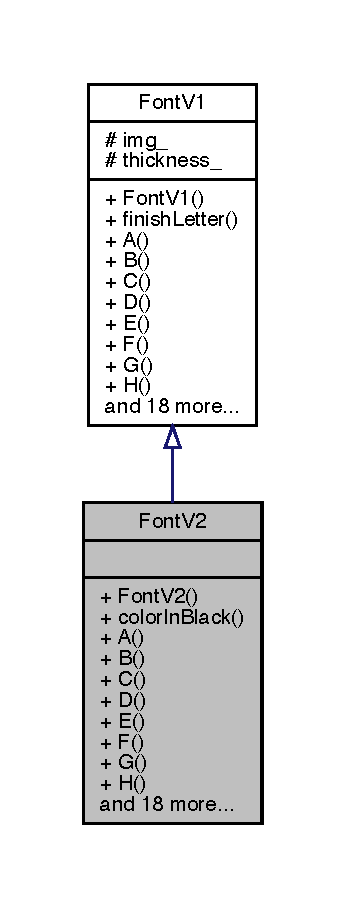
\includegraphics[width=166pt]{class_font_v2__inherit__graph}
\end{center}
\end{figure}


Collaboration diagram for Font\+V2\+:\nopagebreak
\begin{figure}[H]
\begin{center}
\leavevmode
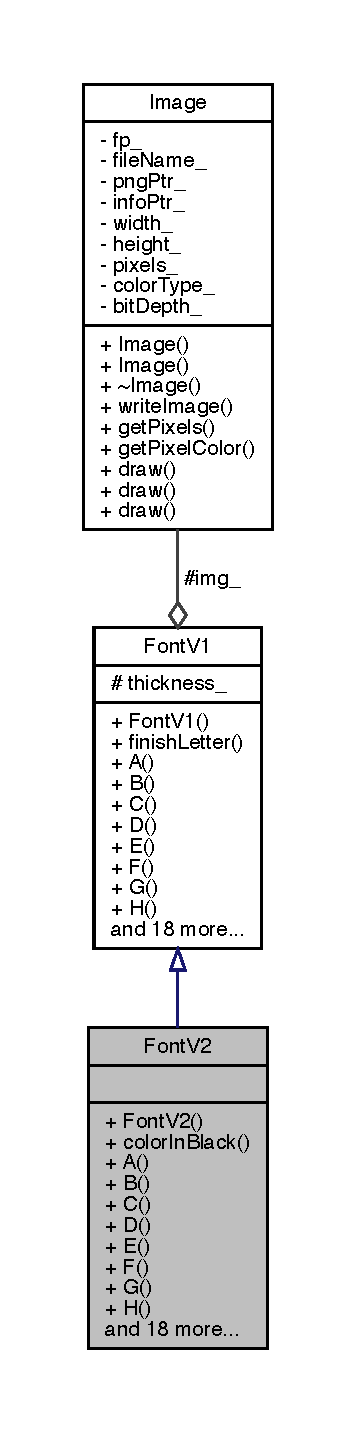
\includegraphics[height=550pt]{class_font_v2__coll__graph}
\end{center}
\end{figure}
\subsection*{Public Member Functions}
\begin{DoxyCompactItemize}
\item 
\mbox{\hyperlink{class_font_v2_aecf9c03af709aa99c23f5c785e798ef4}{Font\+V2}} (char $\ast$image\+Name)
\begin{DoxyCompactList}\small\item\em Default constructor. \end{DoxyCompactList}\item 
void \mbox{\hyperlink{class_font_v2_a04f2501961bc286ce70fbb6a840b0e8a}{color\+In\+Black}} (int x, int y)
\begin{DoxyCompactList}\small\item\em Color the inside of a letter. \end{DoxyCompactList}\item 
void \mbox{\hyperlink{class_font_v2_ae1a96e014f4cc9e4447b0a2d947f4a33}{A}} ()
\begin{DoxyCompactList}\small\item\em Draw the letter A in black on the \mbox{\hyperlink{class_image}{Image}}. \end{DoxyCompactList}\item 
void \mbox{\hyperlink{class_font_v2_a0a895c96067874028864303ab64ce889}{B}} ()
\begin{DoxyCompactList}\small\item\em Draw the letter B in black on the \mbox{\hyperlink{class_image}{Image}}. \end{DoxyCompactList}\item 
void \mbox{\hyperlink{class_font_v2_ab7dc3a07d1442bd391513c4c202f2a43}{C}} ()
\begin{DoxyCompactList}\small\item\em Draw the letter C in black on the \mbox{\hyperlink{class_image}{Image}}. \end{DoxyCompactList}\item 
void \mbox{\hyperlink{class_font_v2_ab6a088abff91bacc1096b6008296142b}{D}} ()
\begin{DoxyCompactList}\small\item\em Draw the letter D in black on the \mbox{\hyperlink{class_image}{Image}}. \end{DoxyCompactList}\item 
void \mbox{\hyperlink{class_font_v2_a3dc7a171c913a94b688689c69abafeca}{E}} ()
\begin{DoxyCompactList}\small\item\em Draw the letter E in black on the \mbox{\hyperlink{class_image}{Image}}. \end{DoxyCompactList}\item 
void \mbox{\hyperlink{class_font_v2_a061b1fab86aa9bae29fb7460a6ea6401}{F}} ()
\begin{DoxyCompactList}\small\item\em Draw the letter F in black on the \mbox{\hyperlink{class_image}{Image}}. \end{DoxyCompactList}\item 
void \mbox{\hyperlink{class_font_v2_a27ece9cc80af5c5d32cad07f00ed714c}{G}} ()
\begin{DoxyCompactList}\small\item\em Draw the letter G in black on the \mbox{\hyperlink{class_image}{Image}}. \end{DoxyCompactList}\item 
void \mbox{\hyperlink{class_font_v2_af03f8d436cc22f57b2bdd471b265896e}{H}} ()
\begin{DoxyCompactList}\small\item\em Draw the letter H in black on the \mbox{\hyperlink{class_image}{Image}}. \end{DoxyCompactList}\item 
void \mbox{\hyperlink{class_font_v2_aaace3b75c86f0536789a232f5b38321d}{I}} ()
\begin{DoxyCompactList}\small\item\em Draw the letter I in black on the \mbox{\hyperlink{class_image}{Image}}. \end{DoxyCompactList}\item 
void \mbox{\hyperlink{class_font_v2_a6cc91c88325f086dc95cd733ebda7849}{J}} ()
\begin{DoxyCompactList}\small\item\em Draw the letter J in black on the \mbox{\hyperlink{class_image}{Image}}. \end{DoxyCompactList}\item 
void \mbox{\hyperlink{class_font_v2_a1871c49a753378d2f50ad91ea8b26c10}{K}} ()
\begin{DoxyCompactList}\small\item\em Draw the letter K in black on the \mbox{\hyperlink{class_image}{Image}}. \end{DoxyCompactList}\item 
void \mbox{\hyperlink{class_font_v2_ae40068da683965bc711e752af9acf360}{L}} ()
\begin{DoxyCompactList}\small\item\em Draw the letter L in black on the \mbox{\hyperlink{class_image}{Image}}. \end{DoxyCompactList}\item 
void \mbox{\hyperlink{class_font_v2_a65ab055c8555447a542ed5c26ef925ee}{M}} ()
\begin{DoxyCompactList}\small\item\em Draw the letter M in black on the \mbox{\hyperlink{class_image}{Image}}. \end{DoxyCompactList}\item 
void \mbox{\hyperlink{class_font_v2_ab0f1cbe6375f24c45f6d9bd518165353}{N}} ()
\begin{DoxyCompactList}\small\item\em Draw the letter N in black on the \mbox{\hyperlink{class_image}{Image}}. \end{DoxyCompactList}\item 
void \mbox{\hyperlink{class_font_v2_afb1d85a50e3982f0f1e77d5e1ca7f53c}{O}} ()
\begin{DoxyCompactList}\small\item\em Draw the letter O in black on the \mbox{\hyperlink{class_image}{Image}}. \end{DoxyCompactList}\item 
void \mbox{\hyperlink{class_font_v2_ab47b245b84ea5c1dd89055c83b6ea052}{P}} ()
\begin{DoxyCompactList}\small\item\em Draw the letter P in black on the \mbox{\hyperlink{class_image}{Image}}. \end{DoxyCompactList}\item 
void \mbox{\hyperlink{class_font_v2_af8e979a962becf153ecc82051ad2c8fc}{Q}} ()
\begin{DoxyCompactList}\small\item\em Draw the letter Q in black on the \mbox{\hyperlink{class_image}{Image}}. \end{DoxyCompactList}\item 
void \mbox{\hyperlink{class_font_v2_a852e482795dc7557137419b713711774}{R}} ()
\begin{DoxyCompactList}\small\item\em Draw the letter R in black on the \mbox{\hyperlink{class_image}{Image}}. \end{DoxyCompactList}\item 
void \mbox{\hyperlink{class_font_v2_adcccd6f866d51bb27568d8c4c465551f}{S}} ()
\begin{DoxyCompactList}\small\item\em Draw the letter S in black on the \mbox{\hyperlink{class_image}{Image}}. \end{DoxyCompactList}\item 
void \mbox{\hyperlink{class_font_v2_a0311eabb37bc231b9b0c0a13cdc0e562}{T}} ()
\begin{DoxyCompactList}\small\item\em Draw the letter T in black on the \mbox{\hyperlink{class_image}{Image}}. \end{DoxyCompactList}\item 
void \mbox{\hyperlink{class_font_v2_a893e649c0fccfae9d99322fe5e333369}{U}} ()
\begin{DoxyCompactList}\small\item\em Draw the letter U in black on the \mbox{\hyperlink{class_image}{Image}}. \end{DoxyCompactList}\item 
void \mbox{\hyperlink{class_font_v2_a58980cf432ef60e1a765b1033da310b4}{V}} ()
\begin{DoxyCompactList}\small\item\em Draw the letter V in black on the \mbox{\hyperlink{class_image}{Image}}. \end{DoxyCompactList}\item 
void \mbox{\hyperlink{class_font_v2_abb6c182459f9a1a20c4d6a85d09b1b1d}{W}} ()
\begin{DoxyCompactList}\small\item\em Draw the letter W in black on the \mbox{\hyperlink{class_image}{Image}}. \end{DoxyCompactList}\item 
void \mbox{\hyperlink{class_font_v2_a63545ba2652b9559d8d171c5bd37fbea}{X}} ()
\begin{DoxyCompactList}\small\item\em Draw the letter X in black on the \mbox{\hyperlink{class_image}{Image}}. \end{DoxyCompactList}\item 
void \mbox{\hyperlink{class_font_v2_a858b25a33231fe1a78539d040e59f0ee}{Y}} ()
\begin{DoxyCompactList}\small\item\em Draw the letter Y in black on the \mbox{\hyperlink{class_image}{Image}}. \end{DoxyCompactList}\item 
void \mbox{\hyperlink{class_font_v2_a9650b871667f1c226d6e0e042f311a51}{Z}} ()
\begin{DoxyCompactList}\small\item\em Draw the letter Z in black on the \mbox{\hyperlink{class_image}{Image}}. \end{DoxyCompactList}\end{DoxyCompactItemize}
\subsection*{Additional Inherited Members}


\subsection{Constructor \& Destructor Documentation}
\mbox{\Hypertarget{class_font_v2_aecf9c03af709aa99c23f5c785e798ef4}\label{class_font_v2_aecf9c03af709aa99c23f5c785e798ef4}} 
\index{Font\+V2@{Font\+V2}!Font\+V2@{Font\+V2}}
\index{Font\+V2@{Font\+V2}!Font\+V2@{Font\+V2}}
\subsubsection{\texorpdfstring{Font\+V2()}{FontV2()}}
{\footnotesize\ttfamily Font\+V2\+::\+Font\+V2 (\begin{DoxyParamCaption}\item[{char $\ast$}]{image\+Name }\end{DoxyParamCaption})\hspace{0.3cm}{\ttfamily [inline]}}



Default constructor. 


\begin{DoxyCode}
24 : \mbox{\hyperlink{class_font_v1_ada1ed699d42679f81146af4bc20db006}{FontV1}}(imageName) \{\}
\end{DoxyCode}


\subsection{Member Function Documentation}
\mbox{\Hypertarget{class_font_v2_ae1a96e014f4cc9e4447b0a2d947f4a33}\label{class_font_v2_ae1a96e014f4cc9e4447b0a2d947f4a33}} 
\index{Font\+V2@{Font\+V2}!A@{A}}
\index{A@{A}!Font\+V2@{Font\+V2}}
\subsubsection{\texorpdfstring{A()}{A()}}
{\footnotesize\ttfamily void Font\+V2\+::A (\begin{DoxyParamCaption}{ }\end{DoxyParamCaption})}



Draw the letter A in black on the \mbox{\hyperlink{class_image}{Image}}. 


\begin{DoxyCode}
26                \{
27     \mbox{\hyperlink{class_font_v1_a29afd2079bc41cdec9d3de6bb4e1be52}{FontV1::A}}();
28     \mbox{\hyperlink{class_font_v2_a04f2501961bc286ce70fbb6a840b0e8a}{colorInBlack}}(250, 240);
29 \}
\end{DoxyCode}
\mbox{\Hypertarget{class_font_v2_a0a895c96067874028864303ab64ce889}\label{class_font_v2_a0a895c96067874028864303ab64ce889}} 
\index{Font\+V2@{Font\+V2}!B@{B}}
\index{B@{B}!Font\+V2@{Font\+V2}}
\subsubsection{\texorpdfstring{B()}{B()}}
{\footnotesize\ttfamily void Font\+V2\+::B (\begin{DoxyParamCaption}{ }\end{DoxyParamCaption})}



Draw the letter B in black on the \mbox{\hyperlink{class_image}{Image}}. 


\begin{DoxyCode}
31                \{
32     \mbox{\hyperlink{class_font_v1_a620ee7876d479807f73481f27be48f2a}{FontV1::B}}();
33     \mbox{\hyperlink{class_font_v2_a04f2501961bc286ce70fbb6a840b0e8a}{colorInBlack}}(250, 160);
34 \}
\end{DoxyCode}
\mbox{\Hypertarget{class_font_v2_ab7dc3a07d1442bd391513c4c202f2a43}\label{class_font_v2_ab7dc3a07d1442bd391513c4c202f2a43}} 
\index{Font\+V2@{Font\+V2}!C@{C}}
\index{C@{C}!Font\+V2@{Font\+V2}}
\subsubsection{\texorpdfstring{C()}{C()}}
{\footnotesize\ttfamily void Font\+V2\+::C (\begin{DoxyParamCaption}{ }\end{DoxyParamCaption})}



Draw the letter C in black on the \mbox{\hyperlink{class_image}{Image}}. 


\begin{DoxyCode}
36                \{
37     \mbox{\hyperlink{class_font_v1_a80602716ae6907fa518fbb50eeda2515}{FontV1::C}}();
38     \mbox{\hyperlink{class_font_v2_a04f2501961bc286ce70fbb6a840b0e8a}{colorInBlack}}(250, 160);
39 \}
\end{DoxyCode}
\mbox{\Hypertarget{class_font_v2_a04f2501961bc286ce70fbb6a840b0e8a}\label{class_font_v2_a04f2501961bc286ce70fbb6a840b0e8a}} 
\index{Font\+V2@{Font\+V2}!color\+In\+Black@{color\+In\+Black}}
\index{color\+In\+Black@{color\+In\+Black}!Font\+V2@{Font\+V2}}
\subsubsection{\texorpdfstring{color\+In\+Black()}{colorInBlack()}}
{\footnotesize\ttfamily void Font\+V2\+::color\+In\+Black (\begin{DoxyParamCaption}\item[{int}]{x,  }\item[{int}]{y }\end{DoxyParamCaption})}



Color the inside of a letter. 

Perform Seed fill Algorithm to transform the white pixel inside the contour into black pixel 
\begin{DoxyParams}{Parameters}
{\em x} & coordinate \\
\hline
{\em y} & coordinate \\
\hline
\end{DoxyParams}

\begin{DoxyCode}
12                                       \{
13     \textcolor{keywordflow}{if} ((x <= 100 || x >= 400) || (y <= 100 || y >= 400)) \{
14         \textcolor{keywordflow}{return};
15     \}
16     \textcolor{keywordtype}{unsigned} \textcolor{keywordtype}{int}* color = \mbox{\hyperlink{class_font_v1_a00569e3e3c4b70f437b63f396f735fb0}{img\_}}.\mbox{\hyperlink{class_image_adb23176701dae47479d4919f55f3aec5}{getPixelColor}}(\mbox{\hyperlink{class_point}{Point}}(x,y));
17     \textcolor{keywordflow}{if} (color[0] == 255 \&\& color[1] == 255 \&\& color[2] == 255) \{
18         \mbox{\hyperlink{class_font_v1_a00569e3e3c4b70f437b63f396f735fb0}{img\_}}.\mbox{\hyperlink{class_image_a8d162f3cab956131d58708c09aa560b0}{draw}}(\mbox{\hyperlink{class_point}{Point}}(x, y, 0, 0, 0));
19         \mbox{\hyperlink{class_font_v2_a04f2501961bc286ce70fbb6a840b0e8a}{colorInBlack}}(x+1, y);
20         \mbox{\hyperlink{class_font_v2_a04f2501961bc286ce70fbb6a840b0e8a}{colorInBlack}}(x-1, y);
21         \mbox{\hyperlink{class_font_v2_a04f2501961bc286ce70fbb6a840b0e8a}{colorInBlack}}(x, y+1);
22         \mbox{\hyperlink{class_font_v2_a04f2501961bc286ce70fbb6a840b0e8a}{colorInBlack}}(x, y-1);
23     \}
24 \}
\end{DoxyCode}
\mbox{\Hypertarget{class_font_v2_ab6a088abff91bacc1096b6008296142b}\label{class_font_v2_ab6a088abff91bacc1096b6008296142b}} 
\index{Font\+V2@{Font\+V2}!D@{D}}
\index{D@{D}!Font\+V2@{Font\+V2}}
\subsubsection{\texorpdfstring{D()}{D()}}
{\footnotesize\ttfamily void Font\+V2\+::D (\begin{DoxyParamCaption}{ }\end{DoxyParamCaption})}



Draw the letter D in black on the \mbox{\hyperlink{class_image}{Image}}. 


\begin{DoxyCode}
41                \{
42     \mbox{\hyperlink{class_font_v1_a3f4558aabfef6e0783c2294aecf215d0}{FontV1::D}}();
43     \mbox{\hyperlink{class_font_v2_a04f2501961bc286ce70fbb6a840b0e8a}{colorInBlack}}(250, 160);
44 \}
\end{DoxyCode}
\mbox{\Hypertarget{class_font_v2_a3dc7a171c913a94b688689c69abafeca}\label{class_font_v2_a3dc7a171c913a94b688689c69abafeca}} 
\index{Font\+V2@{Font\+V2}!E@{E}}
\index{E@{E}!Font\+V2@{Font\+V2}}
\subsubsection{\texorpdfstring{E()}{E()}}
{\footnotesize\ttfamily void Font\+V2\+::E (\begin{DoxyParamCaption}{ }\end{DoxyParamCaption})}



Draw the letter E in black on the \mbox{\hyperlink{class_image}{Image}}. 


\begin{DoxyCode}
46                \{
47     \mbox{\hyperlink{class_font_v1_ab8a34299af7a36cfd94c2691b579a0fa}{FontV1::E}}();
48     \mbox{\hyperlink{class_font_v2_a04f2501961bc286ce70fbb6a840b0e8a}{colorInBlack}}(250, 250);
49 \}
\end{DoxyCode}
\mbox{\Hypertarget{class_font_v2_a061b1fab86aa9bae29fb7460a6ea6401}\label{class_font_v2_a061b1fab86aa9bae29fb7460a6ea6401}} 
\index{Font\+V2@{Font\+V2}!F@{F}}
\index{F@{F}!Font\+V2@{Font\+V2}}
\subsubsection{\texorpdfstring{F()}{F()}}
{\footnotesize\ttfamily void Font\+V2\+::F (\begin{DoxyParamCaption}{ }\end{DoxyParamCaption})}



Draw the letter F in black on the \mbox{\hyperlink{class_image}{Image}}. 


\begin{DoxyCode}
51                \{
52     \mbox{\hyperlink{class_font_v1_a40dd925bee9092d13ba1a00546cc7160}{FontV1::F}}();
53     \mbox{\hyperlink{class_font_v2_a04f2501961bc286ce70fbb6a840b0e8a}{colorInBlack}}(250, 250);
54 \}
\end{DoxyCode}
\mbox{\Hypertarget{class_font_v2_a27ece9cc80af5c5d32cad07f00ed714c}\label{class_font_v2_a27ece9cc80af5c5d32cad07f00ed714c}} 
\index{Font\+V2@{Font\+V2}!G@{G}}
\index{G@{G}!Font\+V2@{Font\+V2}}
\subsubsection{\texorpdfstring{G()}{G()}}
{\footnotesize\ttfamily void Font\+V2\+::G (\begin{DoxyParamCaption}{ }\end{DoxyParamCaption})}



Draw the letter G in black on the \mbox{\hyperlink{class_image}{Image}}. 


\begin{DoxyCode}
56                \{
57     \mbox{\hyperlink{class_font_v1_a9806041ba05556826ba6b4a0760fcee4}{FontV1::G}}();
58     \mbox{\hyperlink{class_font_v2_a04f2501961bc286ce70fbb6a840b0e8a}{colorInBlack}}(250, 160);
59 \}
\end{DoxyCode}
\mbox{\Hypertarget{class_font_v2_af03f8d436cc22f57b2bdd471b265896e}\label{class_font_v2_af03f8d436cc22f57b2bdd471b265896e}} 
\index{Font\+V2@{Font\+V2}!H@{H}}
\index{H@{H}!Font\+V2@{Font\+V2}}
\subsubsection{\texorpdfstring{H()}{H()}}
{\footnotesize\ttfamily void Font\+V2\+::H (\begin{DoxyParamCaption}{ }\end{DoxyParamCaption})}



Draw the letter H in black on the \mbox{\hyperlink{class_image}{Image}}. 


\begin{DoxyCode}
61                \{
62     \mbox{\hyperlink{class_font_v1_aac6c3d7f8116c21fd9339d07aa63a797}{FontV1::H}}();
63     \mbox{\hyperlink{class_font_v2_a04f2501961bc286ce70fbb6a840b0e8a}{colorInBlack}}(250, 230);
64 \}
\end{DoxyCode}
\mbox{\Hypertarget{class_font_v2_aaace3b75c86f0536789a232f5b38321d}\label{class_font_v2_aaace3b75c86f0536789a232f5b38321d}} 
\index{Font\+V2@{Font\+V2}!I@{I}}
\index{I@{I}!Font\+V2@{Font\+V2}}
\subsubsection{\texorpdfstring{I()}{I()}}
{\footnotesize\ttfamily void Font\+V2\+::I (\begin{DoxyParamCaption}{ }\end{DoxyParamCaption})}



Draw the letter I in black on the \mbox{\hyperlink{class_image}{Image}}. 


\begin{DoxyCode}
66                \{
67     \mbox{\hyperlink{class_font_v1_aab86d5ae867a26e0384c919f82f0bcf1}{FontV1::I}}();
68     \mbox{\hyperlink{class_font_v2_a04f2501961bc286ce70fbb6a840b0e8a}{colorInBlack}}(250, 250);
69 \}
\end{DoxyCode}
\mbox{\Hypertarget{class_font_v2_a6cc91c88325f086dc95cd733ebda7849}\label{class_font_v2_a6cc91c88325f086dc95cd733ebda7849}} 
\index{Font\+V2@{Font\+V2}!J@{J}}
\index{J@{J}!Font\+V2@{Font\+V2}}
\subsubsection{\texorpdfstring{J()}{J()}}
{\footnotesize\ttfamily void Font\+V2\+::J (\begin{DoxyParamCaption}{ }\end{DoxyParamCaption})}



Draw the letter J in black on the \mbox{\hyperlink{class_image}{Image}}. 


\begin{DoxyCode}
71                \{
72     \mbox{\hyperlink{class_font_v1_a3fe315f13fd21c6dbd5f81113cd1c3f6}{FontV1::J}}();
73     \mbox{\hyperlink{class_font_v2_a04f2501961bc286ce70fbb6a840b0e8a}{colorInBlack}}(290, 250);
74 \}
\end{DoxyCode}
\mbox{\Hypertarget{class_font_v2_a1871c49a753378d2f50ad91ea8b26c10}\label{class_font_v2_a1871c49a753378d2f50ad91ea8b26c10}} 
\index{Font\+V2@{Font\+V2}!K@{K}}
\index{K@{K}!Font\+V2@{Font\+V2}}
\subsubsection{\texorpdfstring{K()}{K()}}
{\footnotesize\ttfamily void Font\+V2\+::K (\begin{DoxyParamCaption}{ }\end{DoxyParamCaption})}



Draw the letter K in black on the \mbox{\hyperlink{class_image}{Image}}. 


\begin{DoxyCode}
76                \{
77     \mbox{\hyperlink{class_font_v1_a45ed7d1ac12bd32f458b5b144dd132ba}{FontV1::K}}();
78     \mbox{\hyperlink{class_font_v2_a04f2501961bc286ce70fbb6a840b0e8a}{colorInBlack}}(210, 250);
79 \}
\end{DoxyCode}
\mbox{\Hypertarget{class_font_v2_ae40068da683965bc711e752af9acf360}\label{class_font_v2_ae40068da683965bc711e752af9acf360}} 
\index{Font\+V2@{Font\+V2}!L@{L}}
\index{L@{L}!Font\+V2@{Font\+V2}}
\subsubsection{\texorpdfstring{L()}{L()}}
{\footnotesize\ttfamily void Font\+V2\+::L (\begin{DoxyParamCaption}{ }\end{DoxyParamCaption})}



Draw the letter L in black on the \mbox{\hyperlink{class_image}{Image}}. 


\begin{DoxyCode}
81                \{
82     \mbox{\hyperlink{class_font_v1_a17ba426bfb42af35ea882ab3beeba734}{FontV1::L}}();
83     \mbox{\hyperlink{class_font_v2_a04f2501961bc286ce70fbb6a840b0e8a}{colorInBlack}}(210, 250);
84 \}
\end{DoxyCode}
\mbox{\Hypertarget{class_font_v2_a65ab055c8555447a542ed5c26ef925ee}\label{class_font_v2_a65ab055c8555447a542ed5c26ef925ee}} 
\index{Font\+V2@{Font\+V2}!M@{M}}
\index{M@{M}!Font\+V2@{Font\+V2}}
\subsubsection{\texorpdfstring{M()}{M()}}
{\footnotesize\ttfamily void Font\+V2\+::M (\begin{DoxyParamCaption}{ }\end{DoxyParamCaption})}



Draw the letter M in black on the \mbox{\hyperlink{class_image}{Image}}. 


\begin{DoxyCode}
86                \{
87     \mbox{\hyperlink{class_font_v1_a69afdf545ed6bccbb31efaef5d6d4219}{FontV1::M}}();
88     \mbox{\hyperlink{class_font_v2_a04f2501961bc286ce70fbb6a840b0e8a}{colorInBlack}}(250, 235);
89 \}
\end{DoxyCode}
\mbox{\Hypertarget{class_font_v2_ab0f1cbe6375f24c45f6d9bd518165353}\label{class_font_v2_ab0f1cbe6375f24c45f6d9bd518165353}} 
\index{Font\+V2@{Font\+V2}!N@{N}}
\index{N@{N}!Font\+V2@{Font\+V2}}
\subsubsection{\texorpdfstring{N()}{N()}}
{\footnotesize\ttfamily void Font\+V2\+::N (\begin{DoxyParamCaption}{ }\end{DoxyParamCaption})}



Draw the letter N in black on the \mbox{\hyperlink{class_image}{Image}}. 


\begin{DoxyCode}
91                \{
92     \mbox{\hyperlink{class_font_v1_a725c93ea00d851ca5b43c0d594f1d6d0}{FontV1::N}}();
93     \mbox{\hyperlink{class_font_v2_a04f2501961bc286ce70fbb6a840b0e8a}{colorInBlack}}(250, 250);
94 \}
\end{DoxyCode}
\mbox{\Hypertarget{class_font_v2_afb1d85a50e3982f0f1e77d5e1ca7f53c}\label{class_font_v2_afb1d85a50e3982f0f1e77d5e1ca7f53c}} 
\index{Font\+V2@{Font\+V2}!O@{O}}
\index{O@{O}!Font\+V2@{Font\+V2}}
\subsubsection{\texorpdfstring{O()}{O()}}
{\footnotesize\ttfamily void Font\+V2\+::O (\begin{DoxyParamCaption}{ }\end{DoxyParamCaption})}



Draw the letter O in black on the \mbox{\hyperlink{class_image}{Image}}. 


\begin{DoxyCode}
96                \{
97     \mbox{\hyperlink{class_font_v1_a9338f8d780e9913a848310355973ebf3}{FontV1::O}}();
98     \mbox{\hyperlink{class_font_v2_a04f2501961bc286ce70fbb6a840b0e8a}{colorInBlack}}(250, 160);
99 \}
\end{DoxyCode}
\mbox{\Hypertarget{class_font_v2_ab47b245b84ea5c1dd89055c83b6ea052}\label{class_font_v2_ab47b245b84ea5c1dd89055c83b6ea052}} 
\index{Font\+V2@{Font\+V2}!P@{P}}
\index{P@{P}!Font\+V2@{Font\+V2}}
\subsubsection{\texorpdfstring{P()}{P()}}
{\footnotesize\ttfamily void Font\+V2\+::P (\begin{DoxyParamCaption}{ }\end{DoxyParamCaption})}



Draw the letter P in black on the \mbox{\hyperlink{class_image}{Image}}. 


\begin{DoxyCode}
101                \{
102     \mbox{\hyperlink{class_font_v1_aeaf56ebe48a78aedf53626f50f10ee4d}{FontV1::P}}();
103     \mbox{\hyperlink{class_font_v2_a04f2501961bc286ce70fbb6a840b0e8a}{colorInBlack}}(210, 250);
104 \}
\end{DoxyCode}
\mbox{\Hypertarget{class_font_v2_af8e979a962becf153ecc82051ad2c8fc}\label{class_font_v2_af8e979a962becf153ecc82051ad2c8fc}} 
\index{Font\+V2@{Font\+V2}!Q@{Q}}
\index{Q@{Q}!Font\+V2@{Font\+V2}}
\subsubsection{\texorpdfstring{Q()}{Q()}}
{\footnotesize\ttfamily void Font\+V2\+::Q (\begin{DoxyParamCaption}{ }\end{DoxyParamCaption})}



Draw the letter Q in black on the \mbox{\hyperlink{class_image}{Image}}. 


\begin{DoxyCode}
106                \{
107     \mbox{\hyperlink{class_font_v1_af7ffd76bf02756d0d1e2d3eab4c65c40}{FontV1::Q}}();
108     \mbox{\hyperlink{class_font_v2_a04f2501961bc286ce70fbb6a840b0e8a}{colorInBlack}}(250, 160);
109 \}
\end{DoxyCode}
\mbox{\Hypertarget{class_font_v2_a852e482795dc7557137419b713711774}\label{class_font_v2_a852e482795dc7557137419b713711774}} 
\index{Font\+V2@{Font\+V2}!R@{R}}
\index{R@{R}!Font\+V2@{Font\+V2}}
\subsubsection{\texorpdfstring{R()}{R()}}
{\footnotesize\ttfamily void Font\+V2\+::R (\begin{DoxyParamCaption}{ }\end{DoxyParamCaption})}



Draw the letter R in black on the \mbox{\hyperlink{class_image}{Image}}. 


\begin{DoxyCode}
111                \{
112     \mbox{\hyperlink{class_font_v1_ab3f9a7e62f7d08792d9028da68f5787e}{FontV1::R}}();
113     \mbox{\hyperlink{class_font_v2_a04f2501961bc286ce70fbb6a840b0e8a}{colorInBlack}}(210, 250);
114 \}
\end{DoxyCode}
\mbox{\Hypertarget{class_font_v2_adcccd6f866d51bb27568d8c4c465551f}\label{class_font_v2_adcccd6f866d51bb27568d8c4c465551f}} 
\index{Font\+V2@{Font\+V2}!S@{S}}
\index{S@{S}!Font\+V2@{Font\+V2}}
\subsubsection{\texorpdfstring{S()}{S()}}
{\footnotesize\ttfamily void Font\+V2\+::S (\begin{DoxyParamCaption}{ }\end{DoxyParamCaption})}



Draw the letter S in black on the \mbox{\hyperlink{class_image}{Image}}. 


\begin{DoxyCode}
116                \{
117     \mbox{\hyperlink{class_font_v1_ab6daa08377051d5af458003c665cfc09}{FontV1::S}}();
118     \mbox{\hyperlink{class_font_v2_a04f2501961bc286ce70fbb6a840b0e8a}{colorInBlack}}(250, 250);
119 \}
\end{DoxyCode}
\mbox{\Hypertarget{class_font_v2_a0311eabb37bc231b9b0c0a13cdc0e562}\label{class_font_v2_a0311eabb37bc231b9b0c0a13cdc0e562}} 
\index{Font\+V2@{Font\+V2}!T@{T}}
\index{T@{T}!Font\+V2@{Font\+V2}}
\subsubsection{\texorpdfstring{T()}{T()}}
{\footnotesize\ttfamily void Font\+V2\+::T (\begin{DoxyParamCaption}{ }\end{DoxyParamCaption})}



Draw the letter T in black on the \mbox{\hyperlink{class_image}{Image}}. 


\begin{DoxyCode}
121                \{
122     \mbox{\hyperlink{class_font_v1_ab520e2522e89b6ff20e42621080edd7d}{FontV1::T}}();
123     \mbox{\hyperlink{class_font_v2_a04f2501961bc286ce70fbb6a840b0e8a}{colorInBlack}}(250, 250);
124 \}
\end{DoxyCode}
\mbox{\Hypertarget{class_font_v2_a893e649c0fccfae9d99322fe5e333369}\label{class_font_v2_a893e649c0fccfae9d99322fe5e333369}} 
\index{Font\+V2@{Font\+V2}!U@{U}}
\index{U@{U}!Font\+V2@{Font\+V2}}
\subsubsection{\texorpdfstring{U()}{U()}}
{\footnotesize\ttfamily void Font\+V2\+::U (\begin{DoxyParamCaption}{ }\end{DoxyParamCaption})}



Draw the letter U in black on the \mbox{\hyperlink{class_image}{Image}}. 


\begin{DoxyCode}
126                \{
127     \mbox{\hyperlink{class_font_v1_a460d625b76b123ba4e67a21091d7dcce}{FontV1::U}}();
128     \mbox{\hyperlink{class_font_v2_a04f2501961bc286ce70fbb6a840b0e8a}{colorInBlack}}(250, 160);
129 \}
\end{DoxyCode}
\mbox{\Hypertarget{class_font_v2_a58980cf432ef60e1a765b1033da310b4}\label{class_font_v2_a58980cf432ef60e1a765b1033da310b4}} 
\index{Font\+V2@{Font\+V2}!V@{V}}
\index{V@{V}!Font\+V2@{Font\+V2}}
\subsubsection{\texorpdfstring{V()}{V()}}
{\footnotesize\ttfamily void Font\+V2\+::V (\begin{DoxyParamCaption}{ }\end{DoxyParamCaption})}



Draw the letter V in black on the \mbox{\hyperlink{class_image}{Image}}. 


\begin{DoxyCode}
131                \{
132     \mbox{\hyperlink{class_font_v1_aa5937063bd49c25ccd8993d375926fb7}{FontV1::V}}();
133     \mbox{\hyperlink{class_font_v2_a04f2501961bc286ce70fbb6a840b0e8a}{colorInBlack}}(250, 160);
134 \}
\end{DoxyCode}
\mbox{\Hypertarget{class_font_v2_abb6c182459f9a1a20c4d6a85d09b1b1d}\label{class_font_v2_abb6c182459f9a1a20c4d6a85d09b1b1d}} 
\index{Font\+V2@{Font\+V2}!W@{W}}
\index{W@{W}!Font\+V2@{Font\+V2}}
\subsubsection{\texorpdfstring{W()}{W()}}
{\footnotesize\ttfamily void Font\+V2\+::W (\begin{DoxyParamCaption}{ }\end{DoxyParamCaption})}



Draw the letter W in black on the \mbox{\hyperlink{class_image}{Image}}. 


\begin{DoxyCode}
136                \{
137     \mbox{\hyperlink{class_font_v1_aa4e67840b676dfffd3e03d873013174c}{FontV1::W}}();
138     \mbox{\hyperlink{class_font_v2_a04f2501961bc286ce70fbb6a840b0e8a}{colorInBlack}}(250, 340);
139 \}
\end{DoxyCode}
\mbox{\Hypertarget{class_font_v2_a63545ba2652b9559d8d171c5bd37fbea}\label{class_font_v2_a63545ba2652b9559d8d171c5bd37fbea}} 
\index{Font\+V2@{Font\+V2}!X@{X}}
\index{X@{X}!Font\+V2@{Font\+V2}}
\subsubsection{\texorpdfstring{X()}{X()}}
{\footnotesize\ttfamily void Font\+V2\+::X (\begin{DoxyParamCaption}{ }\end{DoxyParamCaption})}



Draw the letter X in black on the \mbox{\hyperlink{class_image}{Image}}. 


\begin{DoxyCode}
141                \{
142     \mbox{\hyperlink{class_font_v1_a8a93144edcf0f9bf1ac9017eb916ff82}{FontV1::X}}();
143     \mbox{\hyperlink{class_font_v2_a04f2501961bc286ce70fbb6a840b0e8a}{colorInBlack}}(250, 250);
144 \}
\end{DoxyCode}
\mbox{\Hypertarget{class_font_v2_a858b25a33231fe1a78539d040e59f0ee}\label{class_font_v2_a858b25a33231fe1a78539d040e59f0ee}} 
\index{Font\+V2@{Font\+V2}!Y@{Y}}
\index{Y@{Y}!Font\+V2@{Font\+V2}}
\subsubsection{\texorpdfstring{Y()}{Y()}}
{\footnotesize\ttfamily void Font\+V2\+::Y (\begin{DoxyParamCaption}{ }\end{DoxyParamCaption})}



Draw the letter Y in black on the \mbox{\hyperlink{class_image}{Image}}. 


\begin{DoxyCode}
146                \{
147     \mbox{\hyperlink{class_font_v1_a25827e105e44581040d8c17cc821e4f3}{FontV1::Y}}();
148     \mbox{\hyperlink{class_font_v2_a04f2501961bc286ce70fbb6a840b0e8a}{colorInBlack}}(250, 250);
149 \}
\end{DoxyCode}
\mbox{\Hypertarget{class_font_v2_a9650b871667f1c226d6e0e042f311a51}\label{class_font_v2_a9650b871667f1c226d6e0e042f311a51}} 
\index{Font\+V2@{Font\+V2}!Z@{Z}}
\index{Z@{Z}!Font\+V2@{Font\+V2}}
\subsubsection{\texorpdfstring{Z()}{Z()}}
{\footnotesize\ttfamily void Font\+V2\+::Z (\begin{DoxyParamCaption}{ }\end{DoxyParamCaption})}



Draw the letter Z in black on the \mbox{\hyperlink{class_image}{Image}}. 


\begin{DoxyCode}
151                \{
152     \mbox{\hyperlink{class_font_v1_a10df574bc5aa14a43988d42db4e89504}{FontV1::Z}}();
153     \mbox{\hyperlink{class_font_v2_a04f2501961bc286ce70fbb6a840b0e8a}{colorInBlack}}(250, 160);
154 \}
\end{DoxyCode}


The documentation for this class was generated from the following files\+:\begin{DoxyCompactItemize}
\item 
/\+Users/\+Kevin\+Xu/\+Documents/\+Ecole\+\_\+\+Ingé/2\+A/\+S3/\+P\+A\+P/\+P\+A\+P\+\_\+\+Project/\+Projet/src/\mbox{\hyperlink{_font_v2_8h}{Font\+V2.\+h}}\item 
/\+Users/\+Kevin\+Xu/\+Documents/\+Ecole\+\_\+\+Ingé/2\+A/\+S3/\+P\+A\+P/\+P\+A\+P\+\_\+\+Project/\+Projet/src/\mbox{\hyperlink{_font_v2_8cpp}{Font\+V2.\+cpp}}\end{DoxyCompactItemize}

\hypertarget{class_image}{}\section{Image Class Reference}
\label{class_image}\index{Image@{Image}}


{\ttfamily \#include $<$Image.\+h$>$}



Collaboration diagram for Image\+:
\nopagebreak
\begin{figure}[H]
\begin{center}
\leavevmode
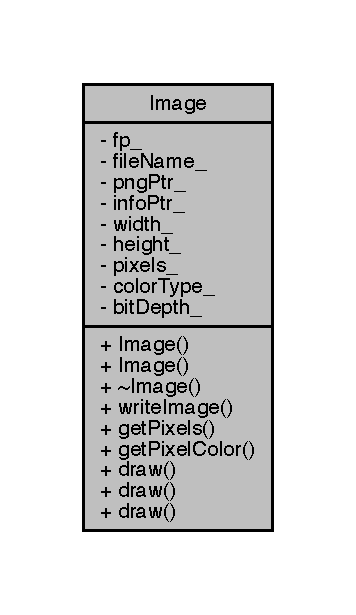
\includegraphics[width=171pt]{class_image__coll__graph}
\end{center}
\end{figure}
\subsection*{Public Member Functions}
\begin{DoxyCompactItemize}
\item 
\mbox{\hyperlink{class_image_a742d8eafbcfe7e0b66a145bac182adb3}{Image}} (char $\ast$file\+Name, int width, int height)
\begin{DoxyCompactList}\small\item\em Valued constructor. \end{DoxyCompactList}\item 
\mbox{\hyperlink{class_image_a7d0a9bb68362e0ec28d5d2c600cc9b59}{Image}} (const \mbox{\hyperlink{class_image}{Image}} \&P)
\begin{DoxyCompactList}\small\item\em Copy-\/constructor. \end{DoxyCompactList}\item 
\mbox{\hyperlink{class_image_a0294f63700543e11c0f0da85601c7ae5}{$\sim$\+Image}} ()
\begin{DoxyCompactList}\small\item\em Destructor. \end{DoxyCompactList}\item 
void \mbox{\hyperlink{class_image_ac34bdffd357a50025e6a72deb02596b5}{write\+Image}} ()
\begin{DoxyCompactList}\small\item\em Produce the image. \end{DoxyCompactList}\item 
png\+\_\+bytep $\ast$ \mbox{\hyperlink{class_image_a434149170df3e6fad24cc123c8ff029d}{get\+Pixels}} () const
\begin{DoxyCompactList}\small\item\em Getter for pixels\+\_\+. \end{DoxyCompactList}\item 
unsigned int $\ast$ \mbox{\hyperlink{class_image_adb23176701dae47479d4919f55f3aec5}{get\+Pixel\+Color}} (\mbox{\hyperlink{class_point}{Point}} P)
\begin{DoxyCompactList}\small\item\em Get the R\+GB level intensity of a pixel. \end{DoxyCompactList}\item 
void \mbox{\hyperlink{class_image_a8d162f3cab956131d58708c09aa560b0}{draw}} (\mbox{\hyperlink{class_point}{Point}} P)
\begin{DoxyCompactList}\small\item\em Setter for pixels\+\_\+. \end{DoxyCompactList}\item 
void \mbox{\hyperlink{class_image_aecc7a0365eb204dba714a71bcb86361d}{draw}} (std\+::vector$<$ \mbox{\hyperlink{class_point}{Point}} $>$ points)
\begin{DoxyCompactList}\small\item\em Draw the points in the vector. \end{DoxyCompactList}\item 
void \mbox{\hyperlink{class_image_a6349aee8ec05bbecb9b6e6430de07d7c}{draw}} (std\+::vector$<$ \mbox{\hyperlink{class_bezier_curve}{Bezier\+Curve}} $>$ curves)
\begin{DoxyCompactList}\small\item\em Draw the Bezier curves. \end{DoxyCompactList}\end{DoxyCompactItemize}
\subsection*{Private Attributes}
\begin{DoxyCompactItemize}
\item 
F\+I\+LE $\ast$ \mbox{\hyperlink{class_image_a4d43b19efb469f7c9fb65e7202d7ba7f}{fp\+\_\+}}
\item 
char $\ast$ \mbox{\hyperlink{class_image_a1f1849b27396edcc169e7d717ef0e6ab}{file\+Name\+\_\+}}
\item 
png\+\_\+structp \mbox{\hyperlink{class_image_aaf607d2596bac09b13370599d9ba6d8c}{png\+Ptr\+\_\+}}
\item 
png\+\_\+infop \mbox{\hyperlink{class_image_a505878e5e19500e3cc1b940067faa584}{info\+Ptr\+\_\+}}
\item 
int \mbox{\hyperlink{class_image_a4c2d8a01ecf1b7438f57f93357080e08}{width\+\_\+}}
\item 
int \mbox{\hyperlink{class_image_a64a699c5bb8e8a18c6971a8032806dba}{height\+\_\+}}
\item 
png\+\_\+bytep $\ast$ \mbox{\hyperlink{class_image_a51351c8507499d09cb9667c20ef01faf}{pixels\+\_\+}}
\end{DoxyCompactItemize}
\subsection*{Static Private Attributes}
\begin{DoxyCompactItemize}
\item 
static const png\+\_\+byte \mbox{\hyperlink{class_image_a94b0dece808a9f06ebb6f4394e8e3048}{color\+Type\+\_\+}} = P\+N\+G\+\_\+\+C\+O\+L\+O\+R\+\_\+\+T\+Y\+P\+E\+\_\+\+R\+GB
\item 
static const png\+\_\+byte \mbox{\hyperlink{class_image_ae472f0390f64eb5d49f858ce95e09ce8}{bit\+Depth\+\_\+}} = 8
\end{DoxyCompactItemize}


\subsection{Constructor \& Destructor Documentation}
\mbox{\Hypertarget{class_image_a742d8eafbcfe7e0b66a145bac182adb3}\label{class_image_a742d8eafbcfe7e0b66a145bac182adb3}} 
\index{Image@{Image}!Image@{Image}}
\index{Image@{Image}!Image@{Image}}
\subsubsection{\texorpdfstring{Image()}{Image()}\hspace{0.1cm}{\footnotesize\ttfamily [1/2]}}
{\footnotesize\ttfamily Image\+::\+Image (\begin{DoxyParamCaption}\item[{char $\ast$}]{file\+Name,  }\item[{int}]{width,  }\item[{int}]{height }\end{DoxyParamCaption})}



Valued constructor. 


\begin{DoxyParams}{Parameters}
{\em x} & coordinate \\
\hline
{\em y} & coordinate \\
\hline
\end{DoxyParams}

\begin{DoxyCode}
11                                                   \{
12     \textcolor{comment}{// File creation}
13     \mbox{\hyperlink{class_image_a1f1849b27396edcc169e7d717ef0e6ab}{fileName\_}} = fileName;
14     \mbox{\hyperlink{class_image_a4d43b19efb469f7c9fb65e7202d7ba7f}{fp\_}} = fopen(fileName, \textcolor{stringliteral}{"wb"}); 
15     \textcolor{keywordflow}{if} (!\mbox{\hyperlink{class_image_a4d43b19efb469f7c9fb65e7202d7ba7f}{fp\_}}) \{
16         std::cout << \textcolor{stringliteral}{"Erreur de creation du fichier"} << std::endl;
17         abort();
18     \}
19 
20     \textcolor{comment}{// png\_structp creation}
21     \mbox{\hyperlink{class_image_aaf607d2596bac09b13370599d9ba6d8c}{pngPtr\_}} = png\_create\_write\_struct(PNG\_LIBPNG\_VER\_STRING, NULL, NULL, NULL);
22     \textcolor{keywordflow}{if} (!\mbox{\hyperlink{class_image_aaf607d2596bac09b13370599d9ba6d8c}{pngPtr\_}}) \{
23         fclose(\mbox{\hyperlink{class_image_a4d43b19efb469f7c9fb65e7202d7ba7f}{fp\_}});
24         std::cout << \textcolor{stringliteral}{"Erreur de creation png\_structp"} << std::endl;
25         abort();
26     \}
27 
28     \mbox{\hyperlink{class_image_a505878e5e19500e3cc1b940067faa584}{infoPtr\_}} = png\_create\_info\_struct(\mbox{\hyperlink{class_image_aaf607d2596bac09b13370599d9ba6d8c}{pngPtr\_}}); 
29     \textcolor{keywordflow}{if} (!\mbox{\hyperlink{class_image_a505878e5e19500e3cc1b940067faa584}{infoPtr\_}}) \{
30         png\_destroy\_write\_struct(\&\mbox{\hyperlink{class_image_aaf607d2596bac09b13370599d9ba6d8c}{pngPtr\_}}, NULL);
31         fclose(\mbox{\hyperlink{class_image_a4d43b19efb469f7c9fb65e7202d7ba7f}{fp\_}});
32         std::cout << \textcolor{stringliteral}{"Erreur de creation png\_infop"} << std::endl;
33         abort(); \textcolor{comment}{//return 1; }
34     \}
35 
36     \textcolor{keywordflow}{if} (setjmp(png\_jmpbuf(\mbox{\hyperlink{class_image_aaf607d2596bac09b13370599d9ba6d8c}{pngPtr\_}}))) \{
37         png\_destroy\_write\_struct(\&\mbox{\hyperlink{class_image_aaf607d2596bac09b13370599d9ba6d8c}{pngPtr\_}}, \&\mbox{\hyperlink{class_image_a505878e5e19500e3cc1b940067faa584}{infoPtr\_}}); 
38         fclose(\mbox{\hyperlink{class_image_a4d43b19efb469f7c9fb65e7202d7ba7f}{fp\_}});
39         std::cout << \textcolor{stringliteral}{"Erreur sepjmp"} << std::endl;
40         abort(); \textcolor{comment}{//return 1; }
41     \}
42 
43     png\_init\_io(\mbox{\hyperlink{class_image_aaf607d2596bac09b13370599d9ba6d8c}{pngPtr\_}}, \mbox{\hyperlink{class_image_a4d43b19efb469f7c9fb65e7202d7ba7f}{fp\_}});
44 
45     \textcolor{comment}{// Output is 8bit depth, RGBA format.}
46 
47     \textcolor{comment}{// Image Info}
48     \mbox{\hyperlink{class_image_a4c2d8a01ecf1b7438f57f93357080e08}{width\_}} = width;
49     \mbox{\hyperlink{class_image_a64a699c5bb8e8a18c6971a8032806dba}{height\_}} = height;
50 
51     png\_set\_IHDR(
52         \mbox{\hyperlink{class_image_aaf607d2596bac09b13370599d9ba6d8c}{pngPtr\_}}, 
53         \mbox{\hyperlink{class_image_a505878e5e19500e3cc1b940067faa584}{infoPtr\_}}, 
54         \mbox{\hyperlink{class_image_a4c2d8a01ecf1b7438f57f93357080e08}{width\_}}, 
55         \mbox{\hyperlink{class_image_a64a699c5bb8e8a18c6971a8032806dba}{height\_}}, 
56         \mbox{\hyperlink{class_image_ae472f0390f64eb5d49f858ce95e09ce8}{bitDepth\_}}, 
57         \mbox{\hyperlink{class_image_a94b0dece808a9f06ebb6f4394e8e3048}{colorType\_}}, 
58         PNG\_INTERLACE\_NONE, 
59         PNG\_COMPRESSION\_TYPE\_DEFAULT, 
60         PNG\_FILTER\_TYPE\_DEFAULT
61     );
62     png\_write\_info(\mbox{\hyperlink{class_image_aaf607d2596bac09b13370599d9ba6d8c}{pngPtr\_}}, \mbox{\hyperlink{class_image_a505878e5e19500e3cc1b940067faa584}{infoPtr\_}});
63 
64     \mbox{\hyperlink{class_image_a51351c8507499d09cb9667c20ef01faf}{pixels\_}} = (png\_bytep*) malloc(\mbox{\hyperlink{class_image_a64a699c5bb8e8a18c6971a8032806dba}{height\_}} * \textcolor{keyword}{sizeof}(png\_bytep));
65     \textcolor{comment}{// Allocate memory for one row (3 bytes per pixel - RGB)}
66     \textcolor{keywordflow}{for} (\textcolor{keywordtype}{int} y = 0; y < \mbox{\hyperlink{class_image_a64a699c5bb8e8a18c6971a8032806dba}{height\_}}; y++) \{
67         \mbox{\hyperlink{class_image_a51351c8507499d09cb9667c20ef01faf}{pixels\_}}[y] = (png\_byte*) malloc(3 * \mbox{\hyperlink{class_image_a4c2d8a01ecf1b7438f57f93357080e08}{width\_}} * \textcolor{keyword}{sizeof}(png\_byte));
68     \}
69 
70     \textcolor{comment}{// Set white background}
71     \textcolor{keywordflow}{for} (\textcolor{keywordtype}{int} y = 0; y < \mbox{\hyperlink{class_image_a64a699c5bb8e8a18c6971a8032806dba}{height\_}}; y++) \{
72         png\_bytep row = \mbox{\hyperlink{class_image_a51351c8507499d09cb9667c20ef01faf}{pixels\_}}[y];
73         \textcolor{keywordflow}{for}(\textcolor{keywordtype}{int} x = 0; x < \mbox{\hyperlink{class_image_a4c2d8a01ecf1b7438f57f93357080e08}{width\_}}; x++) \{
74             png\_bytep px = \&(row[x * 3]);
75             px[0] = 255;
76             px[1] = 255;
77             px[2] = 255;
78         \}
79     \}
80 \}
\end{DoxyCode}
\mbox{\Hypertarget{class_image_a7d0a9bb68362e0ec28d5d2c600cc9b59}\label{class_image_a7d0a9bb68362e0ec28d5d2c600cc9b59}} 
\index{Image@{Image}!Image@{Image}}
\index{Image@{Image}!Image@{Image}}
\subsubsection{\texorpdfstring{Image()}{Image()}\hspace{0.1cm}{\footnotesize\ttfamily [2/2]}}
{\footnotesize\ttfamily Image\+::\+Image (\begin{DoxyParamCaption}\item[{const \mbox{\hyperlink{class_image}{Image}} \&}]{P }\end{DoxyParamCaption})}



Copy-\/constructor. 


\begin{DoxyParams}{Parameters}
{\em P} & \mbox{\hyperlink{class_point}{Point}} \\
\hline
\end{DoxyParams}
\mbox{\Hypertarget{class_image_a0294f63700543e11c0f0da85601c7ae5}\label{class_image_a0294f63700543e11c0f0da85601c7ae5}} 
\index{Image@{Image}!````~Image@{$\sim$\+Image}}
\index{````~Image@{$\sim$\+Image}!Image@{Image}}
\subsubsection{\texorpdfstring{$\sim$\+Image()}{~Image()}}
{\footnotesize\ttfamily Image\+::$\sim$\+Image (\begin{DoxyParamCaption}{ }\end{DoxyParamCaption})}



Destructor. 


\begin{DoxyCode}
84               \{
85     \textcolor{comment}{// Freeing memory and closing}
86     \textcolor{keywordflow}{for} (\textcolor{keywordtype}{int} y = 0; y < \mbox{\hyperlink{class_image_a64a699c5bb8e8a18c6971a8032806dba}{height\_}}; y++) \{
87         free(\mbox{\hyperlink{class_image_a51351c8507499d09cb9667c20ef01faf}{pixels\_}}[y]);
88       \}
89     free(\mbox{\hyperlink{class_image_a51351c8507499d09cb9667c20ef01faf}{pixels\_}});
90     fclose(\mbox{\hyperlink{class_image_a4d43b19efb469f7c9fb65e7202d7ba7f}{fp\_}});
91     \textcolor{keywordflow}{if} (\mbox{\hyperlink{class_image_aaf607d2596bac09b13370599d9ba6d8c}{pngPtr\_}} \&\& \mbox{\hyperlink{class_image_a505878e5e19500e3cc1b940067faa584}{infoPtr\_}}) \{
92         png\_destroy\_write\_struct(\&\mbox{\hyperlink{class_image_aaf607d2596bac09b13370599d9ba6d8c}{pngPtr\_}}, \&\mbox{\hyperlink{class_image_a505878e5e19500e3cc1b940067faa584}{infoPtr\_}});
93     \}
94 \}
\end{DoxyCode}


\subsection{Member Function Documentation}
\mbox{\Hypertarget{class_image_a8d162f3cab956131d58708c09aa560b0}\label{class_image_a8d162f3cab956131d58708c09aa560b0}} 
\index{Image@{Image}!draw@{draw}}
\index{draw@{draw}!Image@{Image}}
\subsubsection{\texorpdfstring{draw()}{draw()}\hspace{0.1cm}{\footnotesize\ttfamily [1/3]}}
{\footnotesize\ttfamily void Image\+::draw (\begin{DoxyParamCaption}\item[{\mbox{\hyperlink{class_point}{Point}}}]{P }\end{DoxyParamCaption})}



Setter for pixels\+\_\+. 


\begin{DoxyParams}{Parameters}
{\em pixels} & the pixels of the image Draw a point P\\
\hline
\end{DoxyParams}
Modify the pixels on the image to draw a point 
\begin{DoxyParams}{Parameters}
{\em P} & the point to draw \\
\hline
\end{DoxyParams}

\begin{DoxyCode}
115                         \{
116     png\_bytep px = \&(\mbox{\hyperlink{class_image_a51351c8507499d09cb9667c20ef01faf}{pixels\_}}[\mbox{\hyperlink{class_image_a64a699c5bb8e8a18c6971a8032806dba}{height\_}}-P.\mbox{\hyperlink{class_point_a86d10ff46e08462c45b15a8c7ef62d61}{getY}}()][P.\mbox{\hyperlink{class_point_ac9d5859db121c7d1b89ca89266dca0a3}{getX}}() * 3]);
117     \textcolor{keywordtype}{unsigned} \textcolor{keywordtype}{int} *color = P.\mbox{\hyperlink{class_point_a1aa902dd929328baec8c8f6970284ac2}{getColor}}();
118     px[0] = color[0];
119     px[1] = color[1];
120     px[2] = color[2];
121 \}
\end{DoxyCode}
\mbox{\Hypertarget{class_image_aecc7a0365eb204dba714a71bcb86361d}\label{class_image_aecc7a0365eb204dba714a71bcb86361d}} 
\index{Image@{Image}!draw@{draw}}
\index{draw@{draw}!Image@{Image}}
\subsubsection{\texorpdfstring{draw()}{draw()}\hspace{0.1cm}{\footnotesize\ttfamily [2/3]}}
{\footnotesize\ttfamily void Image\+::draw (\begin{DoxyParamCaption}\item[{std\+::vector$<$ \mbox{\hyperlink{class_point}{Point}} $>$}]{points }\end{DoxyParamCaption})}



Draw the points in the vector. 


\begin{DoxyParams}{Parameters}
{\em points} & The list of points \\
\hline
\end{DoxyParams}

\begin{DoxyCode}
123                                         \{
124     \textcolor{keywordflow}{for} (\textcolor{keyword}{auto} it = points.begin(); it != points.end(); it++) \{
125         \mbox{\hyperlink{class_image_a8d162f3cab956131d58708c09aa560b0}{draw}}(*it);
126     \}
127 \}
\end{DoxyCode}
\mbox{\Hypertarget{class_image_a6349aee8ec05bbecb9b6e6430de07d7c}\label{class_image_a6349aee8ec05bbecb9b6e6430de07d7c}} 
\index{Image@{Image}!draw@{draw}}
\index{draw@{draw}!Image@{Image}}
\subsubsection{\texorpdfstring{draw()}{draw()}\hspace{0.1cm}{\footnotesize\ttfamily [3/3]}}
{\footnotesize\ttfamily void Image\+::draw (\begin{DoxyParamCaption}\item[{std\+::vector$<$ \mbox{\hyperlink{class_bezier_curve}{Bezier\+Curve}} $>$}]{curves }\end{DoxyParamCaption})}



Draw the Bezier curves. 


\begin{DoxyParams}{Parameters}
{\em curves} & The curves to draw \\
\hline
\end{DoxyParams}

\begin{DoxyCode}
129                                               \{
130     \textcolor{keywordflow}{for} (\textcolor{keyword}{auto} it = curves.begin(); it != curves.end(); it++) \{
131         \mbox{\hyperlink{class_image_a8d162f3cab956131d58708c09aa560b0}{draw}}(it->getCurvePoints());
132         std::cout << 6 << std::endl;
133     \} 
134 \}
\end{DoxyCode}
\mbox{\Hypertarget{class_image_adb23176701dae47479d4919f55f3aec5}\label{class_image_adb23176701dae47479d4919f55f3aec5}} 
\index{Image@{Image}!get\+Pixel\+Color@{get\+Pixel\+Color}}
\index{get\+Pixel\+Color@{get\+Pixel\+Color}!Image@{Image}}
\subsubsection{\texorpdfstring{get\+Pixel\+Color()}{getPixelColor()}}
{\footnotesize\ttfamily unsigned int $\ast$ Image\+::get\+Pixel\+Color (\begin{DoxyParamCaption}\item[{\mbox{\hyperlink{class_point}{Point}}}]{P }\end{DoxyParamCaption})}



Get the R\+GB level intensity of a pixel. 


\begin{DoxyParams}{Parameters}
{\em P} & The pixel \\
\hline
\end{DoxyParams}
\begin{DoxyReturn}{Returns}
The R\+GB color 
\end{DoxyReturn}

\begin{DoxyCode}
105                                           \{
106     png\_bytep px = \&(\mbox{\hyperlink{class_image_a51351c8507499d09cb9667c20ef01faf}{pixels\_}}[\mbox{\hyperlink{class_image_a64a699c5bb8e8a18c6971a8032806dba}{height\_}}-P.\mbox{\hyperlink{class_point_a86d10ff46e08462c45b15a8c7ef62d61}{getY}}()][P.\mbox{\hyperlink{class_point_ac9d5859db121c7d1b89ca89266dca0a3}{getX}}() * 3]);
107     \textcolor{keywordtype}{unsigned} \textcolor{keywordtype}{int} *color = \textcolor{keyword}{new} \textcolor{keywordtype}{unsigned} \textcolor{keywordtype}{int}[3];
108     color[0] = px[0];
109     color[1] = px[1];
110     color[2] = px[2];
111     \textcolor{keywordflow}{return} color;
112 \}
\end{DoxyCode}
\mbox{\Hypertarget{class_image_a434149170df3e6fad24cc123c8ff029d}\label{class_image_a434149170df3e6fad24cc123c8ff029d}} 
\index{Image@{Image}!get\+Pixels@{get\+Pixels}}
\index{get\+Pixels@{get\+Pixels}!Image@{Image}}
\subsubsection{\texorpdfstring{get\+Pixels()}{getPixels()}}
{\footnotesize\ttfamily png\+\_\+bytep $\ast$ Image\+::get\+Pixels (\begin{DoxyParamCaption}{ }\end{DoxyParamCaption}) const}



Getter for pixels\+\_\+. 

\begin{DoxyReturn}{Returns}
the pixels\+\_\+ ponter 
\end{DoxyReturn}

\begin{DoxyCode}
101                                   \{
102     \textcolor{keywordflow}{return} \mbox{\hyperlink{class_image_a51351c8507499d09cb9667c20ef01faf}{pixels\_}};
103 \}
\end{DoxyCode}
\mbox{\Hypertarget{class_image_ac34bdffd357a50025e6a72deb02596b5}\label{class_image_ac34bdffd357a50025e6a72deb02596b5}} 
\index{Image@{Image}!write\+Image@{write\+Image}}
\index{write\+Image@{write\+Image}!Image@{Image}}
\subsubsection{\texorpdfstring{write\+Image()}{writeImage()}}
{\footnotesize\ttfamily void Image\+::write\+Image (\begin{DoxyParamCaption}{ }\end{DoxyParamCaption})}



Produce the image. 


\begin{DoxyCode}
96                        \{
97     png\_write\_image(\mbox{\hyperlink{class_image_aaf607d2596bac09b13370599d9ba6d8c}{pngPtr\_}}, \mbox{\hyperlink{class_image_a51351c8507499d09cb9667c20ef01faf}{pixels\_}});
98     png\_write\_end(\mbox{\hyperlink{class_image_aaf607d2596bac09b13370599d9ba6d8c}{pngPtr\_}}, NULL);
99 \}
\end{DoxyCode}


\subsection{Member Data Documentation}
\mbox{\Hypertarget{class_image_ae472f0390f64eb5d49f858ce95e09ce8}\label{class_image_ae472f0390f64eb5d49f858ce95e09ce8}} 
\index{Image@{Image}!bit\+Depth\+\_\+@{bit\+Depth\+\_\+}}
\index{bit\+Depth\+\_\+@{bit\+Depth\+\_\+}!Image@{Image}}
\subsubsection{\texorpdfstring{bit\+Depth\+\_\+}{bitDepth\_}}
{\footnotesize\ttfamily const png\+\_\+byte Image\+::bit\+Depth\+\_\+ = 8\hspace{0.3cm}{\ttfamily [static]}, {\ttfamily [private]}}

\mbox{\Hypertarget{class_image_a94b0dece808a9f06ebb6f4394e8e3048}\label{class_image_a94b0dece808a9f06ebb6f4394e8e3048}} 
\index{Image@{Image}!color\+Type\+\_\+@{color\+Type\+\_\+}}
\index{color\+Type\+\_\+@{color\+Type\+\_\+}!Image@{Image}}
\subsubsection{\texorpdfstring{color\+Type\+\_\+}{colorType\_}}
{\footnotesize\ttfamily const png\+\_\+byte Image\+::color\+Type\+\_\+ = P\+N\+G\+\_\+\+C\+O\+L\+O\+R\+\_\+\+T\+Y\+P\+E\+\_\+\+R\+GB\hspace{0.3cm}{\ttfamily [static]}, {\ttfamily [private]}}

\mbox{\Hypertarget{class_image_a1f1849b27396edcc169e7d717ef0e6ab}\label{class_image_a1f1849b27396edcc169e7d717ef0e6ab}} 
\index{Image@{Image}!file\+Name\+\_\+@{file\+Name\+\_\+}}
\index{file\+Name\+\_\+@{file\+Name\+\_\+}!Image@{Image}}
\subsubsection{\texorpdfstring{file\+Name\+\_\+}{fileName\_}}
{\footnotesize\ttfamily char$\ast$ Image\+::file\+Name\+\_\+\hspace{0.3cm}{\ttfamily [private]}}

\mbox{\Hypertarget{class_image_a4d43b19efb469f7c9fb65e7202d7ba7f}\label{class_image_a4d43b19efb469f7c9fb65e7202d7ba7f}} 
\index{Image@{Image}!fp\+\_\+@{fp\+\_\+}}
\index{fp\+\_\+@{fp\+\_\+}!Image@{Image}}
\subsubsection{\texorpdfstring{fp\+\_\+}{fp\_}}
{\footnotesize\ttfamily F\+I\+LE$\ast$ Image\+::fp\+\_\+\hspace{0.3cm}{\ttfamily [private]}}

\mbox{\Hypertarget{class_image_a64a699c5bb8e8a18c6971a8032806dba}\label{class_image_a64a699c5bb8e8a18c6971a8032806dba}} 
\index{Image@{Image}!height\+\_\+@{height\+\_\+}}
\index{height\+\_\+@{height\+\_\+}!Image@{Image}}
\subsubsection{\texorpdfstring{height\+\_\+}{height\_}}
{\footnotesize\ttfamily int Image\+::height\+\_\+\hspace{0.3cm}{\ttfamily [private]}}

\mbox{\Hypertarget{class_image_a505878e5e19500e3cc1b940067faa584}\label{class_image_a505878e5e19500e3cc1b940067faa584}} 
\index{Image@{Image}!info\+Ptr\+\_\+@{info\+Ptr\+\_\+}}
\index{info\+Ptr\+\_\+@{info\+Ptr\+\_\+}!Image@{Image}}
\subsubsection{\texorpdfstring{info\+Ptr\+\_\+}{infoPtr\_}}
{\footnotesize\ttfamily png\+\_\+infop Image\+::info\+Ptr\+\_\+\hspace{0.3cm}{\ttfamily [private]}}

\mbox{\Hypertarget{class_image_a51351c8507499d09cb9667c20ef01faf}\label{class_image_a51351c8507499d09cb9667c20ef01faf}} 
\index{Image@{Image}!pixels\+\_\+@{pixels\+\_\+}}
\index{pixels\+\_\+@{pixels\+\_\+}!Image@{Image}}
\subsubsection{\texorpdfstring{pixels\+\_\+}{pixels\_}}
{\footnotesize\ttfamily png\+\_\+bytep$\ast$ Image\+::pixels\+\_\+\hspace{0.3cm}{\ttfamily [private]}}

\mbox{\Hypertarget{class_image_aaf607d2596bac09b13370599d9ba6d8c}\label{class_image_aaf607d2596bac09b13370599d9ba6d8c}} 
\index{Image@{Image}!png\+Ptr\+\_\+@{png\+Ptr\+\_\+}}
\index{png\+Ptr\+\_\+@{png\+Ptr\+\_\+}!Image@{Image}}
\subsubsection{\texorpdfstring{png\+Ptr\+\_\+}{pngPtr\_}}
{\footnotesize\ttfamily png\+\_\+structp Image\+::png\+Ptr\+\_\+\hspace{0.3cm}{\ttfamily [private]}}

\mbox{\Hypertarget{class_image_a4c2d8a01ecf1b7438f57f93357080e08}\label{class_image_a4c2d8a01ecf1b7438f57f93357080e08}} 
\index{Image@{Image}!width\+\_\+@{width\+\_\+}}
\index{width\+\_\+@{width\+\_\+}!Image@{Image}}
\subsubsection{\texorpdfstring{width\+\_\+}{width\_}}
{\footnotesize\ttfamily int Image\+::width\+\_\+\hspace{0.3cm}{\ttfamily [private]}}



The documentation for this class was generated from the following files\+:\begin{DoxyCompactItemize}
\item 
/\+Users/\+Kevin\+Xu/\+Documents/\+Ecole\+\_\+\+Ingé/2\+A/\+S3/\+P\+A\+P/\+P\+A\+P\+\_\+\+Project/\+Projet/src/\mbox{\hyperlink{_image_8h}{Image.\+h}}\item 
/\+Users/\+Kevin\+Xu/\+Documents/\+Ecole\+\_\+\+Ingé/2\+A/\+S3/\+P\+A\+P/\+P\+A\+P\+\_\+\+Project/\+Projet/src/\mbox{\hyperlink{_image_8cpp}{Image.\+cpp}}\end{DoxyCompactItemize}

\hypertarget{class_point}{}\section{Point Class Reference}
\label{class_point}\index{Point@{Point}}


{\ttfamily \#include $<$Point.\+h$>$}



Collaboration diagram for Point\+:\nopagebreak
\begin{figure}[H]
\begin{center}
\leavevmode
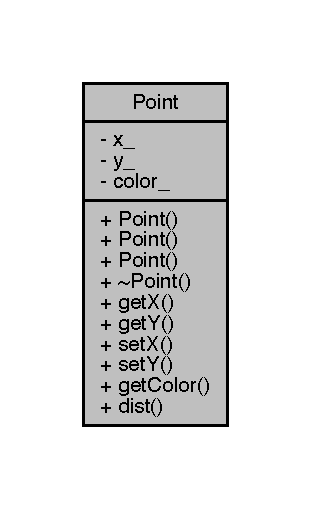
\includegraphics[width=149pt]{class_point__coll__graph}
\end{center}
\end{figure}
\subsection*{Public Member Functions}
\begin{DoxyCompactItemize}
\item 
\mbox{\hyperlink{class_point_ad92f2337b839a94ce97dcdb439b4325a}{Point}} ()
\item 
\mbox{\hyperlink{class_point_af6c52ba545e9d933632b6d4edbf86622}{Point}} (int x, int y, unsigned int R=0, unsigned int G=0, unsigned int B=0)
\begin{DoxyCompactList}\small\item\em Valued constructor. \end{DoxyCompactList}\item 
\mbox{\hyperlink{class_point_a7e32c5a7f878c49ed9f1777b622cc06c}{Point}} (const \mbox{\hyperlink{class_point}{Point}} \&P)
\begin{DoxyCompactList}\small\item\em Copy-\/constructor. \end{DoxyCompactList}\item 
\mbox{\hyperlink{class_point_a395fa04b4ec126b66fc053f829a30cc1}{$\sim$\+Point}} ()
\begin{DoxyCompactList}\small\item\em Destructor. \end{DoxyCompactList}\item 
int \mbox{\hyperlink{class_point_ac9d5859db121c7d1b89ca89266dca0a3}{getX}} () const
\begin{DoxyCompactList}\small\item\em Getter for x. \end{DoxyCompactList}\item 
int \mbox{\hyperlink{class_point_a86d10ff46e08462c45b15a8c7ef62d61}{getY}} () const
\begin{DoxyCompactList}\small\item\em Getter for y\+\_\+. \end{DoxyCompactList}\item 
void \mbox{\hyperlink{class_point_acdc86ab607b2ae8415152883e2629015}{setX}} (int x)
\begin{DoxyCompactList}\small\item\em Setter for x\+\_\+. \end{DoxyCompactList}\item 
void \mbox{\hyperlink{class_point_afccad787a359f062efc1af5e935a99ba}{setY}} (int y)
\begin{DoxyCompactList}\small\item\em Setter for y\+\_\+. \end{DoxyCompactList}\item 
unsigned int $\ast$ \mbox{\hyperlink{class_point_a1aa902dd929328baec8c8f6970284ac2}{get\+Color}} ()
\begin{DoxyCompactList}\small\item\em Getter for color\+\_\+. \end{DoxyCompactList}\item 
double \mbox{\hyperlink{class_point_a31c7abcc57e3a3aefd0724d3c55c52a8}{dist}} (\mbox{\hyperlink{class_point}{Point}} P)
\begin{DoxyCompactList}\small\item\em Euclidian distance between two points. \end{DoxyCompactList}\end{DoxyCompactItemize}
\subsection*{Private Attributes}
\begin{DoxyCompactItemize}
\item 
int \mbox{\hyperlink{class_point_acfe156c55546f7e551fb54c7ea08a6cb}{x\+\_\+}}
\item 
int \mbox{\hyperlink{class_point_ae45effa2adb0036e4a770abb9b1160e6}{y\+\_\+}}
\item 
unsigned int $\ast$ \mbox{\hyperlink{class_point_af3333647d73989850d2fbf64d14eb9cb}{color\+\_\+}}
\end{DoxyCompactItemize}


\subsection{Constructor \& Destructor Documentation}
\mbox{\Hypertarget{class_point_ad92f2337b839a94ce97dcdb439b4325a}\label{class_point_ad92f2337b839a94ce97dcdb439b4325a}} 
\index{Point@{Point}!Point@{Point}}
\index{Point@{Point}!Point@{Point}}
\subsubsection{\texorpdfstring{Point()}{Point()}\hspace{0.1cm}{\footnotesize\ttfamily [1/3]}}
{\footnotesize\ttfamily Point\+::\+Point (\begin{DoxyParamCaption}{ }\end{DoxyParamCaption})}


\begin{DoxyCode}
12              : \mbox{\hyperlink{class_point_acfe156c55546f7e551fb54c7ea08a6cb}{x\_}}(0), \mbox{\hyperlink{class_point_ae45effa2adb0036e4a770abb9b1160e6}{y\_}}(0) \{
13     \mbox{\hyperlink{class_point_af3333647d73989850d2fbf64d14eb9cb}{color\_}} = \textcolor{keyword}{new} \textcolor{keywordtype}{unsigned} \textcolor{keywordtype}{int}[3];
14     \mbox{\hyperlink{class_point_af3333647d73989850d2fbf64d14eb9cb}{color\_}}[0] = 0;
15     \mbox{\hyperlink{class_point_af3333647d73989850d2fbf64d14eb9cb}{color\_}}[1] = 0;
16     \mbox{\hyperlink{class_point_af3333647d73989850d2fbf64d14eb9cb}{color\_}}[2] = 0;
17 \}
\end{DoxyCode}
\mbox{\Hypertarget{class_point_af6c52ba545e9d933632b6d4edbf86622}\label{class_point_af6c52ba545e9d933632b6d4edbf86622}} 
\index{Point@{Point}!Point@{Point}}
\index{Point@{Point}!Point@{Point}}
\subsubsection{\texorpdfstring{Point()}{Point()}\hspace{0.1cm}{\footnotesize\ttfamily [2/3]}}
{\footnotesize\ttfamily Point\+::\+Point (\begin{DoxyParamCaption}\item[{int}]{x,  }\item[{int}]{y,  }\item[{unsigned int}]{R = {\ttfamily 0},  }\item[{unsigned int}]{G = {\ttfamily 0},  }\item[{unsigned int}]{B = {\ttfamily 0} }\end{DoxyParamCaption})}



Valued constructor. 


\begin{DoxyParams}{Parameters}
{\em x} & \mbox{[}description\mbox{]} \\
\hline
{\em y} & \mbox{[}description\mbox{]} \\
\hline
{\em R} & Red level \\
\hline
{\em G} & Green level \\
\hline
{\em B} & Blue level \\
\hline
\end{DoxyParams}

\begin{DoxyCode}
19                                                                          : \mbox{\hyperlink{class_point_acfe156c55546f7e551fb54c7ea08a6cb}{x\_}}(x), 
      \mbox{\hyperlink{class_point_ae45effa2adb0036e4a770abb9b1160e6}{y\_}}(y) \{
20     \mbox{\hyperlink{class_point_af3333647d73989850d2fbf64d14eb9cb}{color\_}} = \textcolor{keyword}{new} \textcolor{keywordtype}{unsigned} \textcolor{keywordtype}{int}[3];
21     \mbox{\hyperlink{class_point_af3333647d73989850d2fbf64d14eb9cb}{color\_}}[0] = R;
22     \mbox{\hyperlink{class_point_af3333647d73989850d2fbf64d14eb9cb}{color\_}}[1] = G;
23     \mbox{\hyperlink{class_point_af3333647d73989850d2fbf64d14eb9cb}{color\_}}[2] = B;
24 \}
\end{DoxyCode}
\mbox{\Hypertarget{class_point_a7e32c5a7f878c49ed9f1777b622cc06c}\label{class_point_a7e32c5a7f878c49ed9f1777b622cc06c}} 
\index{Point@{Point}!Point@{Point}}
\index{Point@{Point}!Point@{Point}}
\subsubsection{\texorpdfstring{Point()}{Point()}\hspace{0.1cm}{\footnotesize\ttfamily [3/3]}}
{\footnotesize\ttfamily Point\+::\+Point (\begin{DoxyParamCaption}\item[{const \mbox{\hyperlink{class_point}{Point}} \&}]{P }\end{DoxyParamCaption})}



Copy-\/constructor. 


\begin{DoxyParams}{Parameters}
{\em P} & \mbox{\hyperlink{class_point}{Point}} \\
\hline
\end{DoxyParams}

\begin{DoxyCode}
26                            : \mbox{\hyperlink{class_point_acfe156c55546f7e551fb54c7ea08a6cb}{x\_}}(P.\mbox{\hyperlink{class_point_acfe156c55546f7e551fb54c7ea08a6cb}{x\_}}), \mbox{\hyperlink{class_point_ae45effa2adb0036e4a770abb9b1160e6}{y\_}}(P.\mbox{\hyperlink{class_point_ae45effa2adb0036e4a770abb9b1160e6}{y\_}}) \{
27     \mbox{\hyperlink{class_point_af3333647d73989850d2fbf64d14eb9cb}{color\_}} = \textcolor{keyword}{new} \textcolor{keywordtype}{unsigned} \textcolor{keywordtype}{int}[3];
28     \mbox{\hyperlink{class_point_af3333647d73989850d2fbf64d14eb9cb}{color\_}}[0] = P.\mbox{\hyperlink{class_point_af3333647d73989850d2fbf64d14eb9cb}{color\_}}[0];
29     \mbox{\hyperlink{class_point_af3333647d73989850d2fbf64d14eb9cb}{color\_}}[1] = P.\mbox{\hyperlink{class_point_af3333647d73989850d2fbf64d14eb9cb}{color\_}}[1];
30     \mbox{\hyperlink{class_point_af3333647d73989850d2fbf64d14eb9cb}{color\_}}[2] = P.\mbox{\hyperlink{class_point_af3333647d73989850d2fbf64d14eb9cb}{color\_}}[2];
31 \}
\end{DoxyCode}
\mbox{\Hypertarget{class_point_a395fa04b4ec126b66fc053f829a30cc1}\label{class_point_a395fa04b4ec126b66fc053f829a30cc1}} 
\index{Point@{Point}!````~Point@{$\sim$\+Point}}
\index{````~Point@{$\sim$\+Point}!Point@{Point}}
\subsubsection{\texorpdfstring{$\sim$\+Point()}{~Point()}}
{\footnotesize\ttfamily Point\+::$\sim$\+Point (\begin{DoxyParamCaption}{ }\end{DoxyParamCaption})}



Destructor. 

Define the default destructor for a matrix. 
\begin{DoxyCode}
34               \{
35     \textcolor{keywordflow}{if} (\mbox{\hyperlink{class_point_af3333647d73989850d2fbf64d14eb9cb}{color\_}}) \{
36         \textcolor{keyword}{delete}[] \mbox{\hyperlink{class_point_af3333647d73989850d2fbf64d14eb9cb}{color\_}};
37     \}
38 \}
\end{DoxyCode}


\subsection{Member Function Documentation}
\mbox{\Hypertarget{class_point_a31c7abcc57e3a3aefd0724d3c55c52a8}\label{class_point_a31c7abcc57e3a3aefd0724d3c55c52a8}} 
\index{Point@{Point}!dist@{dist}}
\index{dist@{dist}!Point@{Point}}
\subsubsection{\texorpdfstring{dist()}{dist()}}
{\footnotesize\ttfamily double Point\+::dist (\begin{DoxyParamCaption}\item[{\mbox{\hyperlink{class_point}{Point}}}]{P }\end{DoxyParamCaption})}



Euclidian distance between two points. 


\begin{DoxyParams}{Parameters}
{\em P} & The other point \\
\hline
\end{DoxyParams}
\begin{DoxyReturn}{Returns}
The euclidian distance 
\end{DoxyReturn}

\begin{DoxyCode}
66                           \{
67     \textcolor{keywordflow}{return} sqrt(pow(\mbox{\hyperlink{class_point_acfe156c55546f7e551fb54c7ea08a6cb}{x\_}} - P.\mbox{\hyperlink{class_point_ac9d5859db121c7d1b89ca89266dca0a3}{getX}}(), 2) + pow(\mbox{\hyperlink{class_point_ae45effa2adb0036e4a770abb9b1160e6}{y\_}} - P.\mbox{\hyperlink{class_point_a86d10ff46e08462c45b15a8c7ef62d61}{getY}}(), 2));
68 \}
\end{DoxyCode}
\mbox{\Hypertarget{class_point_a1aa902dd929328baec8c8f6970284ac2}\label{class_point_a1aa902dd929328baec8c8f6970284ac2}} 
\index{Point@{Point}!get\+Color@{get\+Color}}
\index{get\+Color@{get\+Color}!Point@{Point}}
\subsubsection{\texorpdfstring{get\+Color()}{getColor()}}
{\footnotesize\ttfamily unsigned int$\ast$ Point\+::get\+Color (\begin{DoxyParamCaption}{ }\end{DoxyParamCaption})\hspace{0.3cm}{\ttfamily [inline]}}



Getter for color\+\_\+. 

\begin{DoxyReturn}{Returns}
color\+\_\+ 
\end{DoxyReturn}

\begin{DoxyCode}
71 \{\textcolor{keywordflow}{return} \mbox{\hyperlink{class_point_af3333647d73989850d2fbf64d14eb9cb}{color\_}};\};
\end{DoxyCode}
\mbox{\Hypertarget{class_point_ac9d5859db121c7d1b89ca89266dca0a3}\label{class_point_ac9d5859db121c7d1b89ca89266dca0a3}} 
\index{Point@{Point}!getX@{getX}}
\index{getX@{getX}!Point@{Point}}
\subsubsection{\texorpdfstring{get\+X()}{getX()}}
{\footnotesize\ttfamily int Point\+::getX (\begin{DoxyParamCaption}{ }\end{DoxyParamCaption}) const\hspace{0.3cm}{\ttfamily [inline]}}



Getter for x. 

\begin{DoxyReturn}{Returns}
x\+\_\+ 
\end{DoxyReturn}

\begin{DoxyCode}
47 \{\textcolor{keywordflow}{return} \mbox{\hyperlink{class_point_acfe156c55546f7e551fb54c7ea08a6cb}{x\_}};\}
\end{DoxyCode}
\mbox{\Hypertarget{class_point_a86d10ff46e08462c45b15a8c7ef62d61}\label{class_point_a86d10ff46e08462c45b15a8c7ef62d61}} 
\index{Point@{Point}!getY@{getY}}
\index{getY@{getY}!Point@{Point}}
\subsubsection{\texorpdfstring{get\+Y()}{getY()}}
{\footnotesize\ttfamily int Point\+::getY (\begin{DoxyParamCaption}{ }\end{DoxyParamCaption}) const\hspace{0.3cm}{\ttfamily [inline]}}



Getter for y\+\_\+. 

\begin{DoxyReturn}{Returns}
y\+\_\+ 
\end{DoxyReturn}

\begin{DoxyCode}
53 \{\textcolor{keywordflow}{return} \mbox{\hyperlink{class_point_ae45effa2adb0036e4a770abb9b1160e6}{y\_}};\}
\end{DoxyCode}
\mbox{\Hypertarget{class_point_acdc86ab607b2ae8415152883e2629015}\label{class_point_acdc86ab607b2ae8415152883e2629015}} 
\index{Point@{Point}!setX@{setX}}
\index{setX@{setX}!Point@{Point}}
\subsubsection{\texorpdfstring{set\+X()}{setX()}}
{\footnotesize\ttfamily void Point\+::setX (\begin{DoxyParamCaption}\item[{int}]{x }\end{DoxyParamCaption})}



Setter for x\+\_\+. 


\begin{DoxyParams}{Parameters}
{\em x} & \\
\hline
\end{DoxyParams}

\begin{DoxyCode}
48                       \{
49     \mbox{\hyperlink{class_point_acfe156c55546f7e551fb54c7ea08a6cb}{x\_}} = x;
50 \}
\end{DoxyCode}
\mbox{\Hypertarget{class_point_afccad787a359f062efc1af5e935a99ba}\label{class_point_afccad787a359f062efc1af5e935a99ba}} 
\index{Point@{Point}!setY@{setY}}
\index{setY@{setY}!Point@{Point}}
\subsubsection{\texorpdfstring{set\+Y()}{setY()}}
{\footnotesize\ttfamily void Point\+::setY (\begin{DoxyParamCaption}\item[{int}]{y }\end{DoxyParamCaption})}



Setter for y\+\_\+. 


\begin{DoxyParams}{Parameters}
{\em y} & \\
\hline
\end{DoxyParams}

\begin{DoxyCode}
52                       \{
53     \mbox{\hyperlink{class_point_ae45effa2adb0036e4a770abb9b1160e6}{y\_}} = y;
54 \}
\end{DoxyCode}


\subsection{Member Data Documentation}
\mbox{\Hypertarget{class_point_af3333647d73989850d2fbf64d14eb9cb}\label{class_point_af3333647d73989850d2fbf64d14eb9cb}} 
\index{Point@{Point}!color\+\_\+@{color\+\_\+}}
\index{color\+\_\+@{color\+\_\+}!Point@{Point}}
\subsubsection{\texorpdfstring{color\+\_\+}{color\_}}
{\footnotesize\ttfamily unsigned int$\ast$ Point\+::color\+\_\+\hspace{0.3cm}{\ttfamily [private]}}

\mbox{\Hypertarget{class_point_acfe156c55546f7e551fb54c7ea08a6cb}\label{class_point_acfe156c55546f7e551fb54c7ea08a6cb}} 
\index{Point@{Point}!x\+\_\+@{x\+\_\+}}
\index{x\+\_\+@{x\+\_\+}!Point@{Point}}
\subsubsection{\texorpdfstring{x\+\_\+}{x\_}}
{\footnotesize\ttfamily int Point\+::x\+\_\+\hspace{0.3cm}{\ttfamily [private]}}

\mbox{\Hypertarget{class_point_ae45effa2adb0036e4a770abb9b1160e6}\label{class_point_ae45effa2adb0036e4a770abb9b1160e6}} 
\index{Point@{Point}!y\+\_\+@{y\+\_\+}}
\index{y\+\_\+@{y\+\_\+}!Point@{Point}}
\subsubsection{\texorpdfstring{y\+\_\+}{y\_}}
{\footnotesize\ttfamily int Point\+::y\+\_\+\hspace{0.3cm}{\ttfamily [private]}}



The documentation for this class was generated from the following files\+:\begin{DoxyCompactItemize}
\item 
/\+Users/\+Kevin\+Xu/\+Documents/\+Ecole\+\_\+\+Ingé/2\+A/\+S3/\+P\+A\+P/\+P\+A\+P\+\_\+\+Project/\+Projet/src/\mbox{\hyperlink{_point_8h}{Point.\+h}}\item 
/\+Users/\+Kevin\+Xu/\+Documents/\+Ecole\+\_\+\+Ingé/2\+A/\+S3/\+P\+A\+P/\+P\+A\+P\+\_\+\+Project/\+Projet/src/\mbox{\hyperlink{_point_8cpp}{Point.\+cpp}}\end{DoxyCompactItemize}

\chapter{File Documentation}
\hypertarget{_bezier_curve_8cpp}{}\section{/\+Users/\+Kevin\+Xu/\+Documents/\+Ecole\+\_\+\+Ingé/2\+A/\+S3/\+P\+A\+P/\+P\+A\+P\+\_\+\+Project/\+Projet/src/\+Bezier\+Curve.cpp File Reference}
\label{_bezier_curve_8cpp}\index{/\+Users/\+Kevin\+Xu/\+Documents/\+Ecole\+\_\+\+Ingé/2\+A/\+S3/\+P\+A\+P/\+P\+A\+P\+\_\+\+Project/\+Projet/src/\+Bezier\+Curve.\+cpp@{/\+Users/\+Kevin\+Xu/\+Documents/\+Ecole\+\_\+\+Ingé/2\+A/\+S3/\+P\+A\+P/\+P\+A\+P\+\_\+\+Project/\+Projet/src/\+Bezier\+Curve.\+cpp}}


Class \mbox{\hyperlink{class_bezier_curve}{Bezier\+Curve}} Implementation.  


{\ttfamily \#include $<$iostream$>$}\newline
{\ttfamily \#include $<$cmath$>$}\newline
{\ttfamily \#include \char`\"{}Bezier\+Curve.\+h\char`\"{}}\newline
Include dependency graph for Bezier\+Curve.\+cpp\+:\nopagebreak
\begin{figure}[H]
\begin{center}
\leavevmode
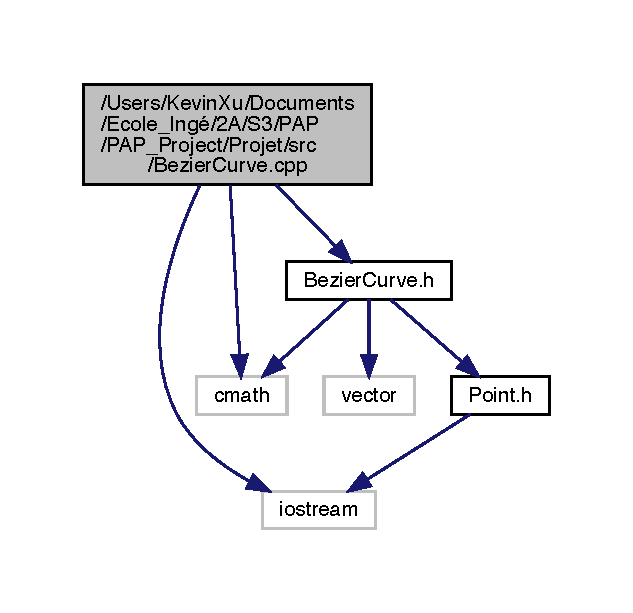
\includegraphics[width=304pt]{_bezier_curve_8cpp__incl}
\end{center}
\end{figure}


\subsection{Detailed Description}
Class \mbox{\hyperlink{class_bezier_curve}{Bezier\+Curve}} Implementation. 

\begin{DoxyAuthor}{Author}
Kevin XU \& Ziheng LI 
\end{DoxyAuthor}
\begin{DoxyDate}{Date}
30 Décembre 2018 
\end{DoxyDate}

\hypertarget{_bezier_curve_8h}{}\section{/\+Users/\+Kevin\+Xu/\+Documents/\+Ecole\+\_\+\+Ingé/2\+A/\+S3/\+P\+A\+P/\+P\+A\+P\+\_\+\+Project/\+Projet/src/\+Bezier\+Curve.h File Reference}
\label{_bezier_curve_8h}\index{/\+Users/\+Kevin\+Xu/\+Documents/\+Ecole\+\_\+\+Ingé/2\+A/\+S3/\+P\+A\+P/\+P\+A\+P\+\_\+\+Project/\+Projet/src/\+Bezier\+Curve.\+h@{/\+Users/\+Kevin\+Xu/\+Documents/\+Ecole\+\_\+\+Ingé/2\+A/\+S3/\+P\+A\+P/\+P\+A\+P\+\_\+\+Project/\+Projet/src/\+Bezier\+Curve.\+h}}


Class \mbox{\hyperlink{class_bezier_curve}{Bezier\+Curve}}.  


{\ttfamily \#include $<$vector$>$}\newline
{\ttfamily \#include $<$cmath$>$}\newline
{\ttfamily \#include \char`\"{}Point.\+h\char`\"{}}\newline
Include dependency graph for Bezier\+Curve.\+h\+:\nopagebreak
\begin{figure}[H]
\begin{center}
\leavevmode
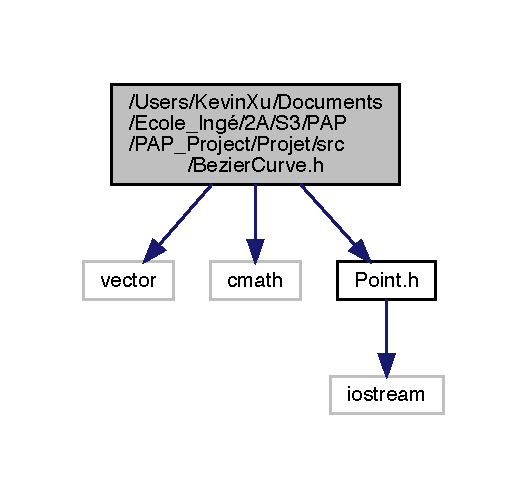
\includegraphics[width=253pt]{_bezier_curve_8h__incl}
\end{center}
\end{figure}
This graph shows which files directly or indirectly include this file\+:\nopagebreak
\begin{figure}[H]
\begin{center}
\leavevmode
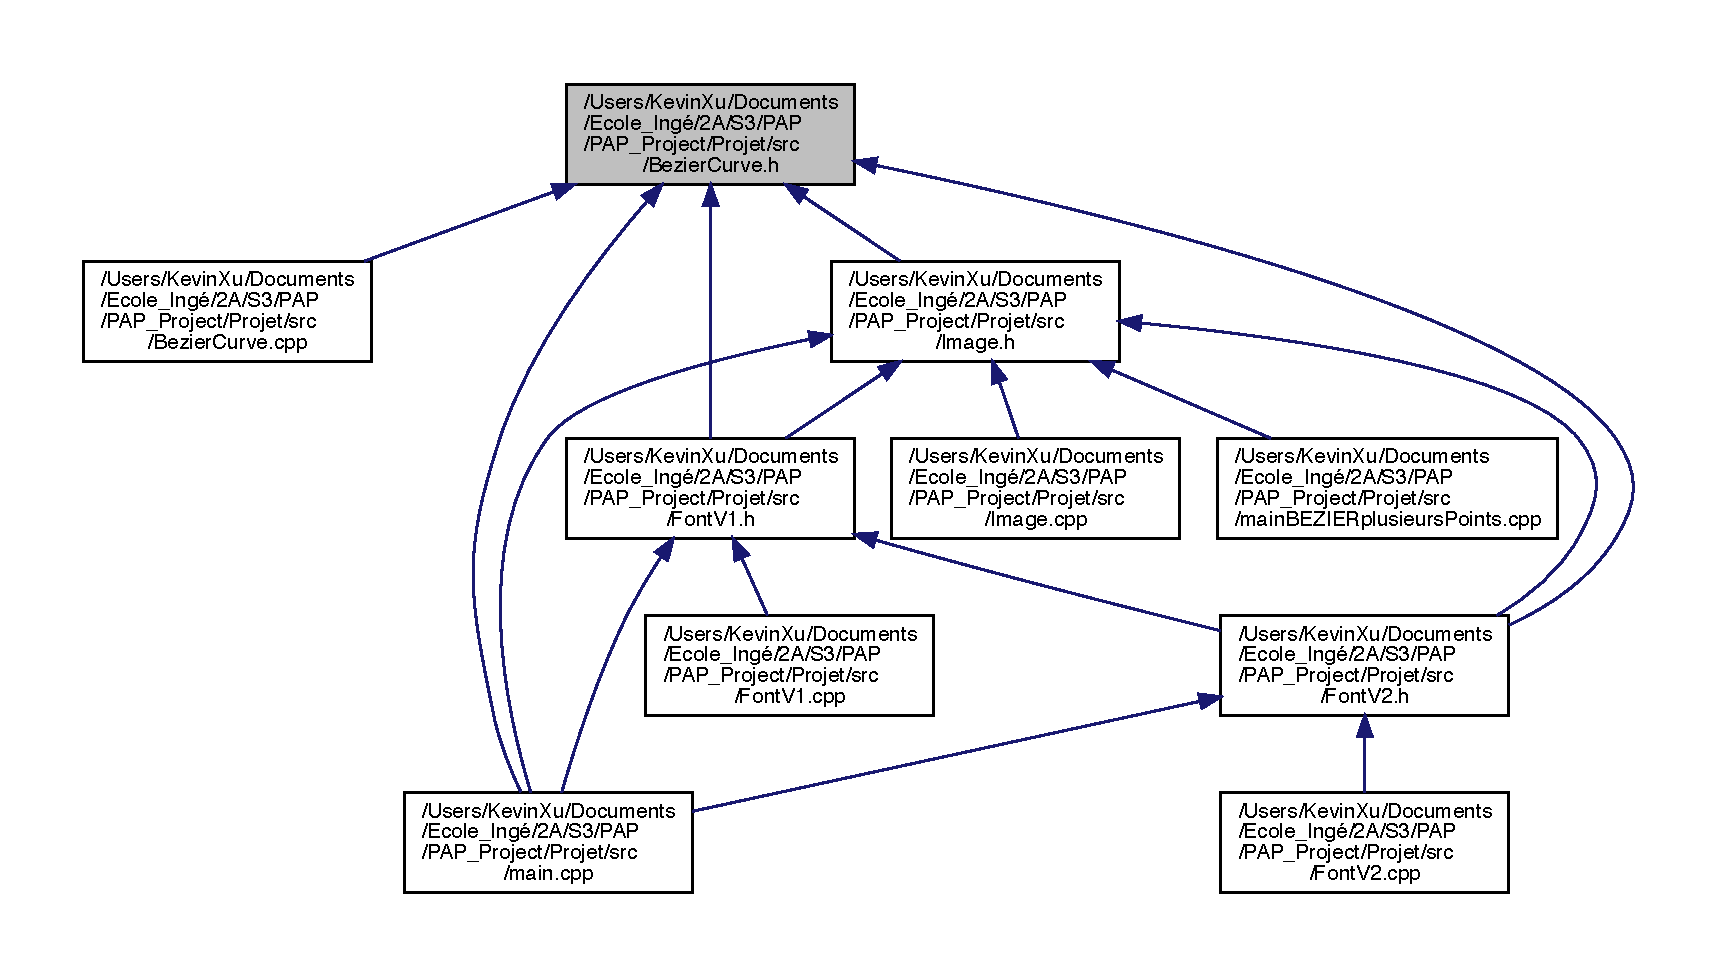
\includegraphics[width=350pt]{_bezier_curve_8h__dep__incl}
\end{center}
\end{figure}
\subsection*{Classes}
\begin{DoxyCompactItemize}
\item 
class \mbox{\hyperlink{class_bezier_curve}{Bezier\+Curve}}
\end{DoxyCompactItemize}


\subsection{Detailed Description}
Class \mbox{\hyperlink{class_bezier_curve}{Bezier\+Curve}}. 

\begin{DoxyAuthor}{Author}
Kevin XU \& Ziheng LI 
\end{DoxyAuthor}
\begin{DoxyDate}{Date}
30 Décembre 
\end{DoxyDate}

\hypertarget{_font_v1_8cpp}{}\section{/\+Users/\+Kevin\+Xu/\+Documents/\+Ecole\+\_\+\+Ingé/2\+A/\+S3/\+P\+A\+P/\+P\+A\+P\+\_\+\+Project/\+Projet/src/\+Font\+V1.cpp File Reference}
\label{_font_v1_8cpp}\index{/\+Users/\+Kevin\+Xu/\+Documents/\+Ecole\+\_\+\+Ingé/2\+A/\+S3/\+P\+A\+P/\+P\+A\+P\+\_\+\+Project/\+Projet/src/\+Font\+V1.\+cpp@{/\+Users/\+Kevin\+Xu/\+Documents/\+Ecole\+\_\+\+Ingé/2\+A/\+S3/\+P\+A\+P/\+P\+A\+P\+\_\+\+Project/\+Projet/src/\+Font\+V1.\+cpp}}


Class \mbox{\hyperlink{class_font_v1}{Font\+V1}}.  


{\ttfamily \#include $<$iostream$>$}\newline
{\ttfamily \#include $<$cmath$>$}\newline
{\ttfamily \#include \char`\"{}Font\+V1.\+h\char`\"{}}\newline
Include dependency graph for Font\+V1.\+cpp\+:
\nopagebreak
\begin{figure}[H]
\begin{center}
\leavevmode
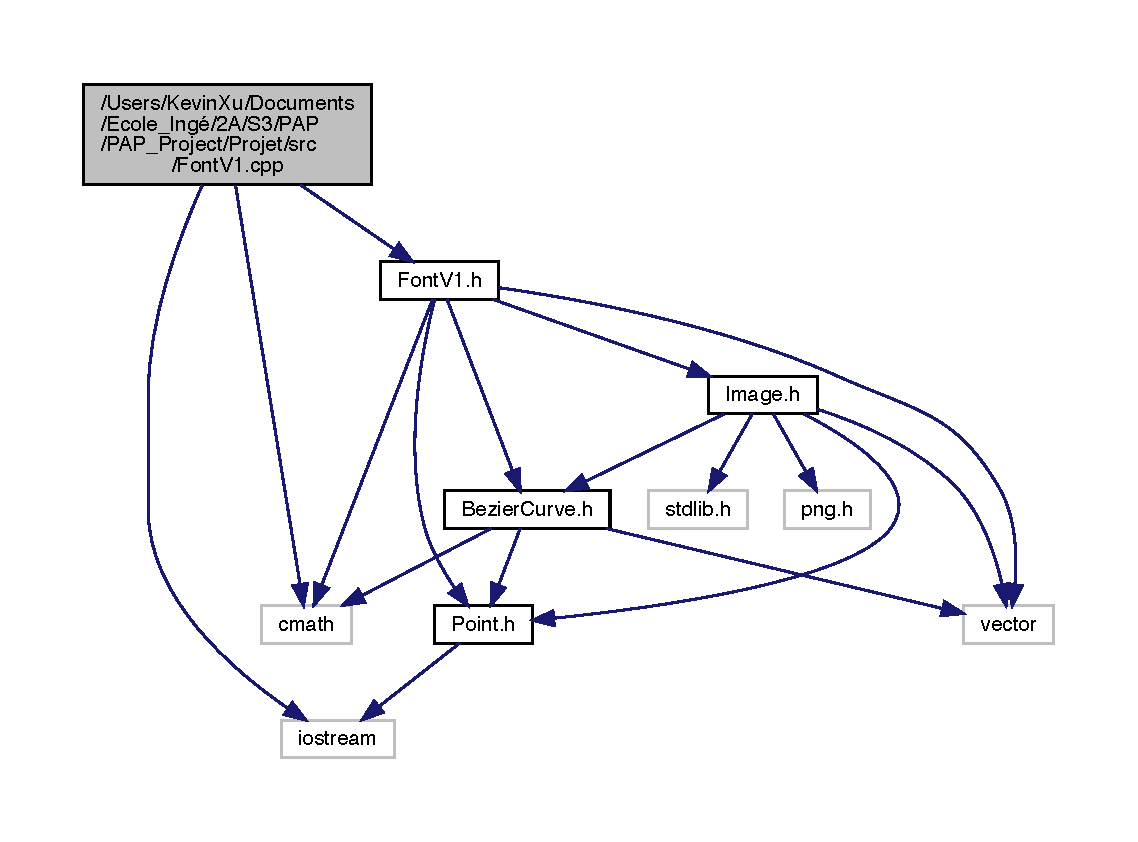
\includegraphics[width=350pt]{_font_v1_8cpp__incl}
\end{center}
\end{figure}


\subsection{Detailed Description}
Class \mbox{\hyperlink{class_font_v1}{Font\+V1}}. 

\begin{DoxyAuthor}{Author}
Kevin XU \& Ziheng LI 
\end{DoxyAuthor}
\begin{DoxyDate}{Date}
31 Décembre 2018 
\end{DoxyDate}

\hypertarget{_font_v1_8h}{}\section{/\+Users/\+Kevin\+Xu/\+Documents/\+Ecole\+\_\+\+Ingé/2\+A/\+S3/\+P\+A\+P/\+P\+A\+P\+\_\+\+Project/\+Projet/src/\+Font\+V1.h File Reference}
\label{_font_v1_8h}\index{/\+Users/\+Kevin\+Xu/\+Documents/\+Ecole\+\_\+\+Ingé/2\+A/\+S3/\+P\+A\+P/\+P\+A\+P\+\_\+\+Project/\+Projet/src/\+Font\+V1.\+h@{/\+Users/\+Kevin\+Xu/\+Documents/\+Ecole\+\_\+\+Ingé/2\+A/\+S3/\+P\+A\+P/\+P\+A\+P\+\_\+\+Project/\+Projet/src/\+Font\+V1.\+h}}


Class \mbox{\hyperlink{class_font_v1}{Font\+V1}}.  


{\ttfamily \#include $<$vector$>$}\newline
{\ttfamily \#include $<$cmath$>$}\newline
{\ttfamily \#include \char`\"{}Point.\+h\char`\"{}}\newline
{\ttfamily \#include \char`\"{}Image.\+h\char`\"{}}\newline
{\ttfamily \#include \char`\"{}Bezier\+Curve.\+h\char`\"{}}\newline
Include dependency graph for Font\+V1.\+h\+:
\nopagebreak
\begin{figure}[H]
\begin{center}
\leavevmode
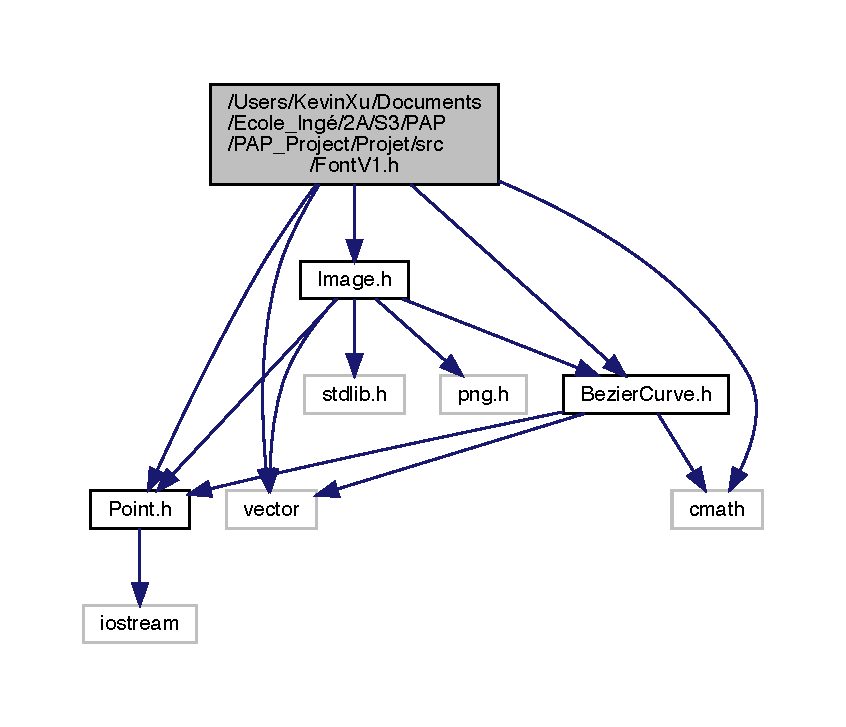
\includegraphics[width=350pt]{_font_v1_8h__incl}
\end{center}
\end{figure}
This graph shows which files directly or indirectly include this file\+:
\nopagebreak
\begin{figure}[H]
\begin{center}
\leavevmode
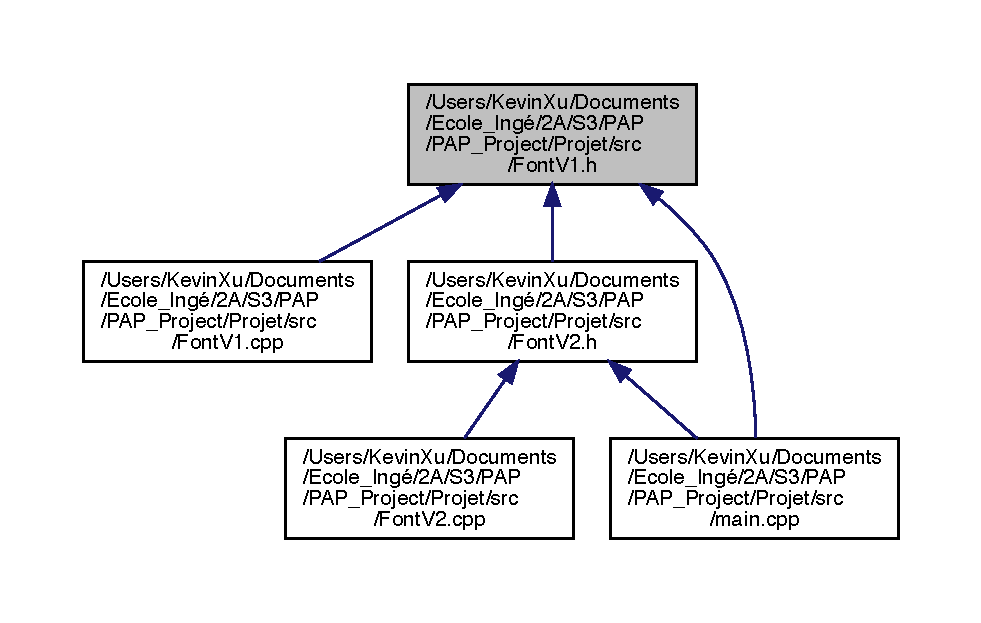
\includegraphics[width=350pt]{_font_v1_8h__dep__incl}
\end{center}
\end{figure}
\subsection*{Classes}
\begin{DoxyCompactItemize}
\item 
class \mbox{\hyperlink{class_font_v1}{Font\+V1}}
\end{DoxyCompactItemize}


\subsection{Detailed Description}
Class \mbox{\hyperlink{class_font_v1}{Font\+V1}}. 

\begin{DoxyAuthor}{Author}
Kevin XU \& Ziheng LI 
\end{DoxyAuthor}
\begin{DoxyDate}{Date}
31 Décembre 2018 
\end{DoxyDate}

\hypertarget{_font_v2_8cpp}{}\section{/\+Users/\+Kevin\+Xu/\+Documents/\+Ecole\+\_\+\+Ingé/2\+A/\+S3/\+P\+A\+P/\+P\+A\+P\+\_\+\+Project/\+Projet/src/\+Font\+V2.cpp File Reference}
\label{_font_v2_8cpp}\index{/\+Users/\+Kevin\+Xu/\+Documents/\+Ecole\+\_\+\+Ingé/2\+A/\+S3/\+P\+A\+P/\+P\+A\+P\+\_\+\+Project/\+Projet/src/\+Font\+V2.\+cpp@{/\+Users/\+Kevin\+Xu/\+Documents/\+Ecole\+\_\+\+Ingé/2\+A/\+S3/\+P\+A\+P/\+P\+A\+P\+\_\+\+Project/\+Projet/src/\+Font\+V2.\+cpp}}


Class \mbox{\hyperlink{class_font_v2}{Font\+V2}}.  


{\ttfamily \#include $<$iostream$>$}\newline
{\ttfamily \#include $<$cmath$>$}\newline
{\ttfamily \#include \char`\"{}Font\+V2.\+h\char`\"{}}\newline
Include dependency graph for Font\+V2.\+cpp\+:
\nopagebreak
\begin{figure}[H]
\begin{center}
\leavevmode
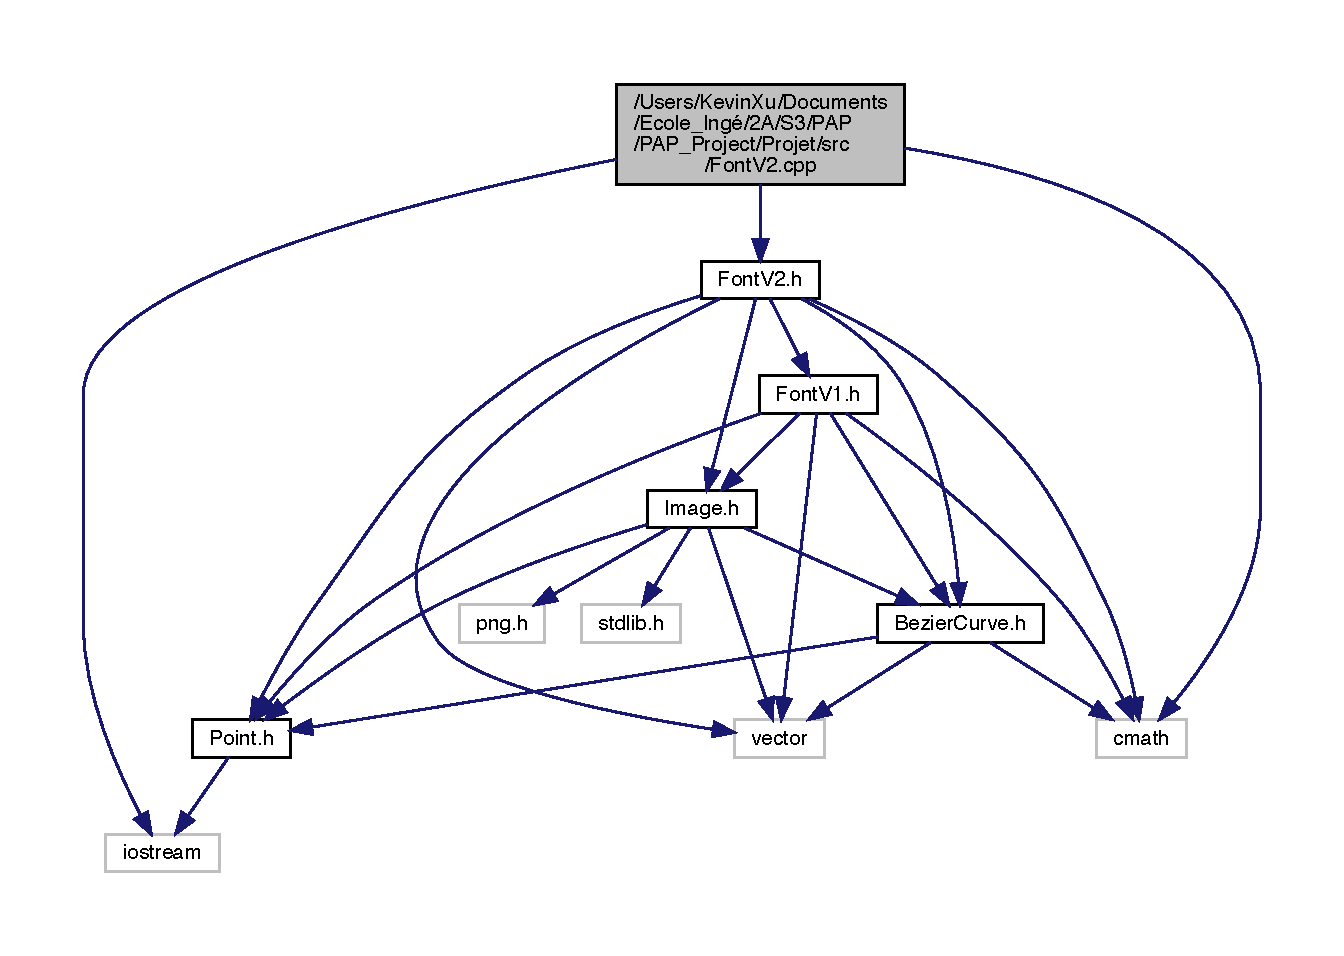
\includegraphics[width=350pt]{_font_v2_8cpp__incl}
\end{center}
\end{figure}


\subsection{Detailed Description}
Class \mbox{\hyperlink{class_font_v2}{Font\+V2}}. 

\begin{DoxyAuthor}{Author}
Kevin XU \& Ziheng LI 
\end{DoxyAuthor}
\begin{DoxyDate}{Date}
5 Janvier 2018 
\end{DoxyDate}

\hypertarget{_font_v2_8h}{}\section{/\+Users/\+Kevin\+Xu/\+Documents/\+Ecole\+\_\+\+Ingé/2\+A/\+S3/\+P\+A\+P/\+P\+A\+P\+\_\+\+Project/\+Projet/src/\+Font\+V2.h File Reference}
\label{_font_v2_8h}\index{/\+Users/\+Kevin\+Xu/\+Documents/\+Ecole\+\_\+\+Ingé/2\+A/\+S3/\+P\+A\+P/\+P\+A\+P\+\_\+\+Project/\+Projet/src/\+Font\+V2.\+h@{/\+Users/\+Kevin\+Xu/\+Documents/\+Ecole\+\_\+\+Ingé/2\+A/\+S3/\+P\+A\+P/\+P\+A\+P\+\_\+\+Project/\+Projet/src/\+Font\+V2.\+h}}


Class \mbox{\hyperlink{class_font_v2}{Font\+V2}}.  


{\ttfamily \#include $<$vector$>$}\newline
{\ttfamily \#include $<$cmath$>$}\newline
{\ttfamily \#include \char`\"{}Point.\+h\char`\"{}}\newline
{\ttfamily \#include \char`\"{}Image.\+h\char`\"{}}\newline
{\ttfamily \#include \char`\"{}Bezier\+Curve.\+h\char`\"{}}\newline
{\ttfamily \#include \char`\"{}Font\+V1.\+h\char`\"{}}\newline
Include dependency graph for Font\+V2.\+h\+:
\nopagebreak
\begin{figure}[H]
\begin{center}
\leavevmode
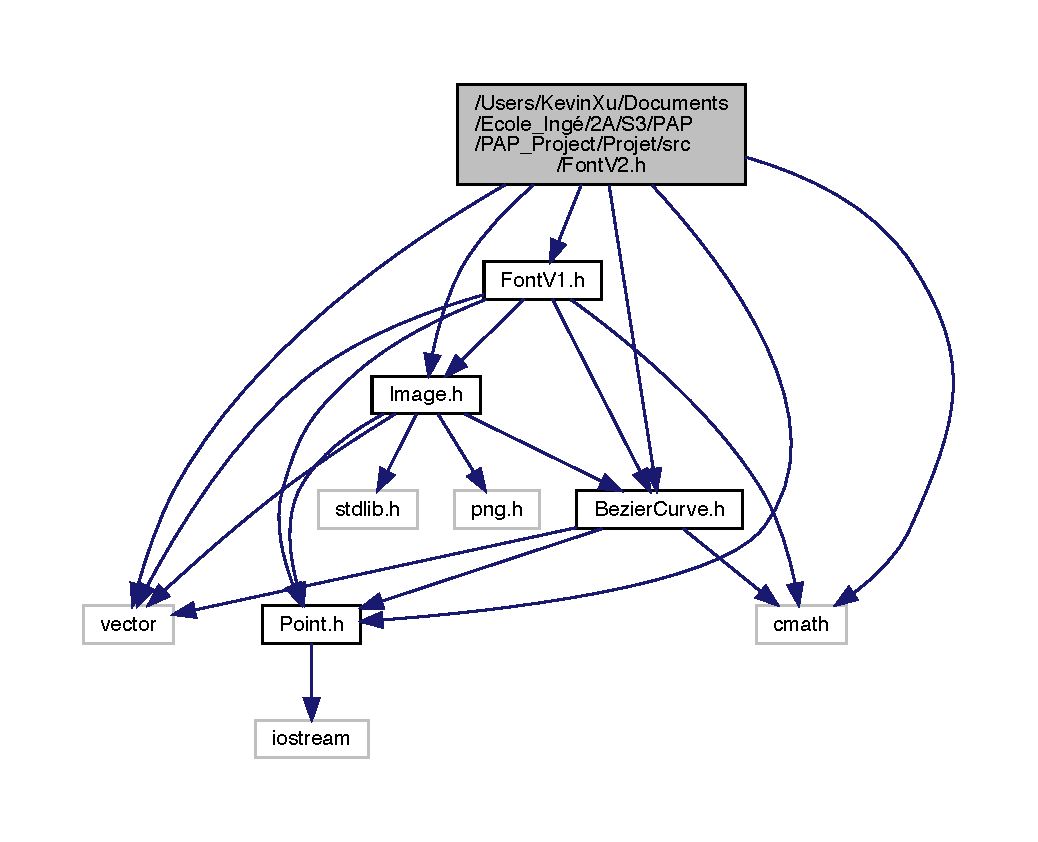
\includegraphics[width=350pt]{_font_v2_8h__incl}
\end{center}
\end{figure}
This graph shows which files directly or indirectly include this file\+:
\nopagebreak
\begin{figure}[H]
\begin{center}
\leavevmode
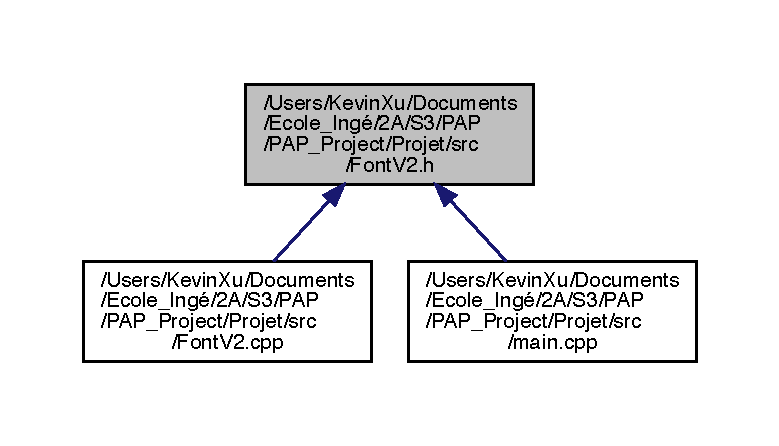
\includegraphics[width=350pt]{_font_v2_8h__dep__incl}
\end{center}
\end{figure}
\subsection*{Classes}
\begin{DoxyCompactItemize}
\item 
class \mbox{\hyperlink{class_font_v2}{Font\+V2}}
\end{DoxyCompactItemize}


\subsection{Detailed Description}
Class \mbox{\hyperlink{class_font_v2}{Font\+V2}}. 

\begin{DoxyAuthor}{Author}
Kevin XU \& Ziheng LI 
\end{DoxyAuthor}
\begin{DoxyDate}{Date}
31 Décembre 2018 
\end{DoxyDate}

\hypertarget{_image_8cpp}{}\section{/\+Users/\+Kevin\+Xu/\+Documents/\+Ecole\+\_\+\+Ingé/2\+A/\+S3/\+P\+A\+P/\+P\+A\+P\+\_\+\+Project/\+Projet/src/\+Image.cpp File Reference}
\label{_image_8cpp}\index{/\+Users/\+Kevin\+Xu/\+Documents/\+Ecole\+\_\+\+Ingé/2\+A/\+S3/\+P\+A\+P/\+P\+A\+P\+\_\+\+Project/\+Projet/src/\+Image.\+cpp@{/\+Users/\+Kevin\+Xu/\+Documents/\+Ecole\+\_\+\+Ingé/2\+A/\+S3/\+P\+A\+P/\+P\+A\+P\+\_\+\+Project/\+Projet/src/\+Image.\+cpp}}


Class \mbox{\hyperlink{class_image}{Image}} Implementation.  


{\ttfamily \#include $<$iostream$>$}\newline
{\ttfamily \#include \char`\"{}Image.\+h\char`\"{}}\newline
Include dependency graph for Image.\+cpp\+:
\nopagebreak
\begin{figure}[H]
\begin{center}
\leavevmode
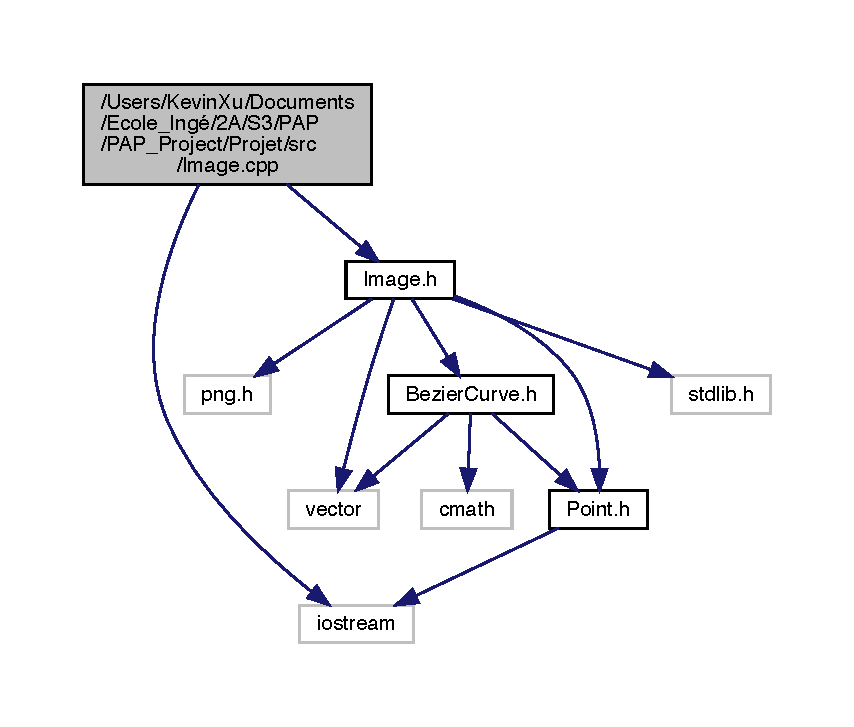
\includegraphics[width=350pt]{_image_8cpp__incl}
\end{center}
\end{figure}


\subsection{Detailed Description}
Class \mbox{\hyperlink{class_image}{Image}} Implementation. 

\begin{DoxyAuthor}{Author}
Kevin XU \& Ziheng LI 
\end{DoxyAuthor}
\begin{DoxyDate}{Date}
30 Novembre 2018 
\end{DoxyDate}

\hypertarget{_image_8h}{}\section{/\+Users/\+Kevin\+Xu/\+Documents/\+Ecole\+\_\+\+Ingé/2\+A/\+S3/\+P\+A\+P/\+P\+A\+P\+\_\+\+Project/\+Projet/src/\+Image.h File Reference}
\label{_image_8h}\index{/\+Users/\+Kevin\+Xu/\+Documents/\+Ecole\+\_\+\+Ingé/2\+A/\+S3/\+P\+A\+P/\+P\+A\+P\+\_\+\+Project/\+Projet/src/\+Image.\+h@{/\+Users/\+Kevin\+Xu/\+Documents/\+Ecole\+\_\+\+Ingé/2\+A/\+S3/\+P\+A\+P/\+P\+A\+P\+\_\+\+Project/\+Projet/src/\+Image.\+h}}


Class \mbox{\hyperlink{class_image}{Image}}.  


{\ttfamily \#include $<$stdlib.\+h$>$}\newline
{\ttfamily \#include $<$png.\+h$>$}\newline
{\ttfamily \#include $<$vector$>$}\newline
{\ttfamily \#include \char`\"{}Point.\+h\char`\"{}}\newline
{\ttfamily \#include \char`\"{}Bezier\+Curve.\+h\char`\"{}}\newline
Include dependency graph for Image.\+h\+:\nopagebreak
\begin{figure}[H]
\begin{center}
\leavevmode
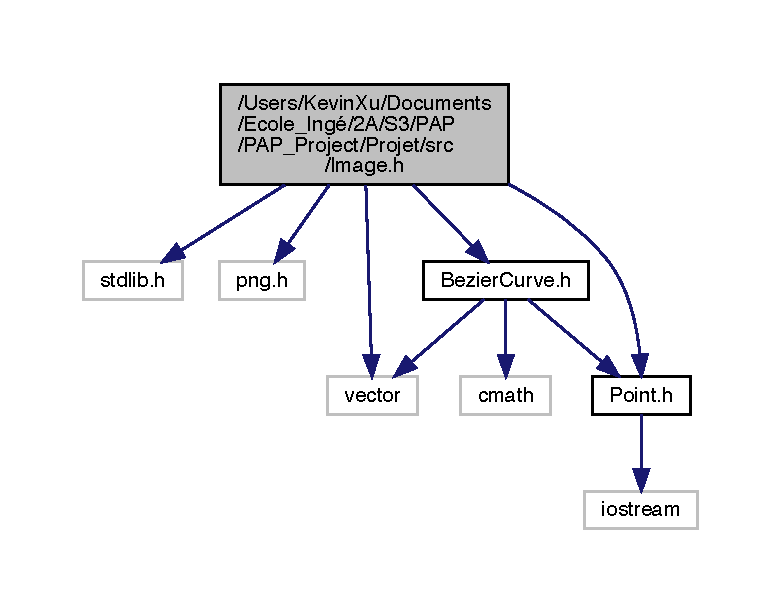
\includegraphics[width=350pt]{_image_8h__incl}
\end{center}
\end{figure}
This graph shows which files directly or indirectly include this file\+:\nopagebreak
\begin{figure}[H]
\begin{center}
\leavevmode
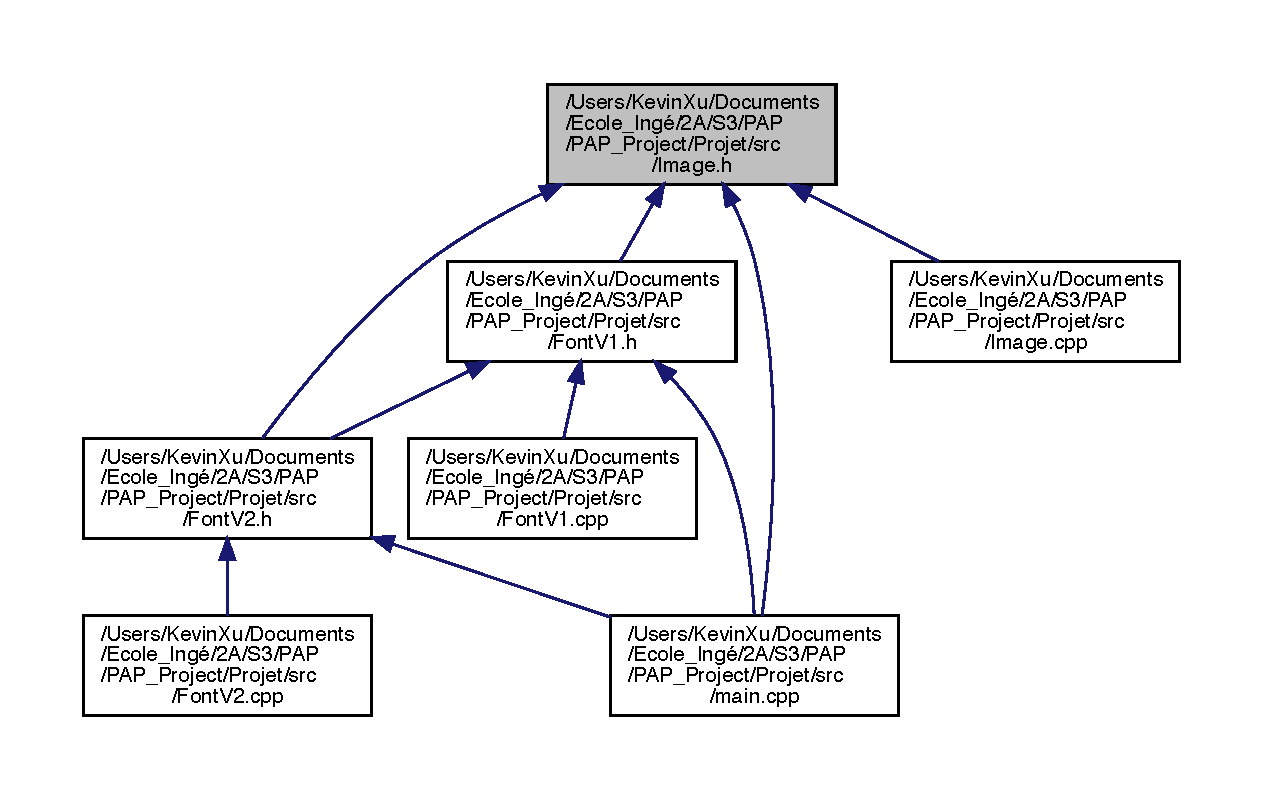
\includegraphics[width=350pt]{_image_8h__dep__incl}
\end{center}
\end{figure}
\subsection*{Classes}
\begin{DoxyCompactItemize}
\item 
class \mbox{\hyperlink{class_image}{Image}}
\end{DoxyCompactItemize}


\subsection{Detailed Description}
Class \mbox{\hyperlink{class_image}{Image}}. 

\begin{DoxyAuthor}{Author}
Kevin XU \& Ziheng LI 
\end{DoxyAuthor}
\begin{DoxyDate}{Date}
30 Novembre 2018 
\end{DoxyDate}

\hypertarget{main_8cpp}{}\section{/\+Users/\+Kevin\+Xu/\+Documents/\+Ecole\+\_\+\+Ingé/2\+A/\+S3/\+P\+A\+P/\+P\+A\+P\+\_\+\+Project/\+Projet/src/main.cpp File Reference}
\label{main_8cpp}\index{/\+Users/\+Kevin\+Xu/\+Documents/\+Ecole\+\_\+\+Ingé/2\+A/\+S3/\+P\+A\+P/\+P\+A\+P\+\_\+\+Project/\+Projet/src/main.\+cpp@{/\+Users/\+Kevin\+Xu/\+Documents/\+Ecole\+\_\+\+Ingé/2\+A/\+S3/\+P\+A\+P/\+P\+A\+P\+\_\+\+Project/\+Projet/src/main.\+cpp}}
{\ttfamily \#include $<$iostream$>$}\newline
{\ttfamily \#include \char`\"{}Point.\+h\char`\"{}}\newline
{\ttfamily \#include \char`\"{}Image.\+h\char`\"{}}\newline
{\ttfamily \#include \char`\"{}Bezier\+Curve.\+h\char`\"{}}\newline
{\ttfamily \#include \char`\"{}Font\+V1.\+h\char`\"{}}\newline
{\ttfamily \#include \char`\"{}Font\+V2.\+h\char`\"{}}\newline
{\ttfamily \#include \char`\"{}Font\+V3.\+h\char`\"{}}\newline
Include dependency graph for main.\+cpp\+:\nopagebreak
\begin{figure}[H]
\begin{center}
\leavevmode
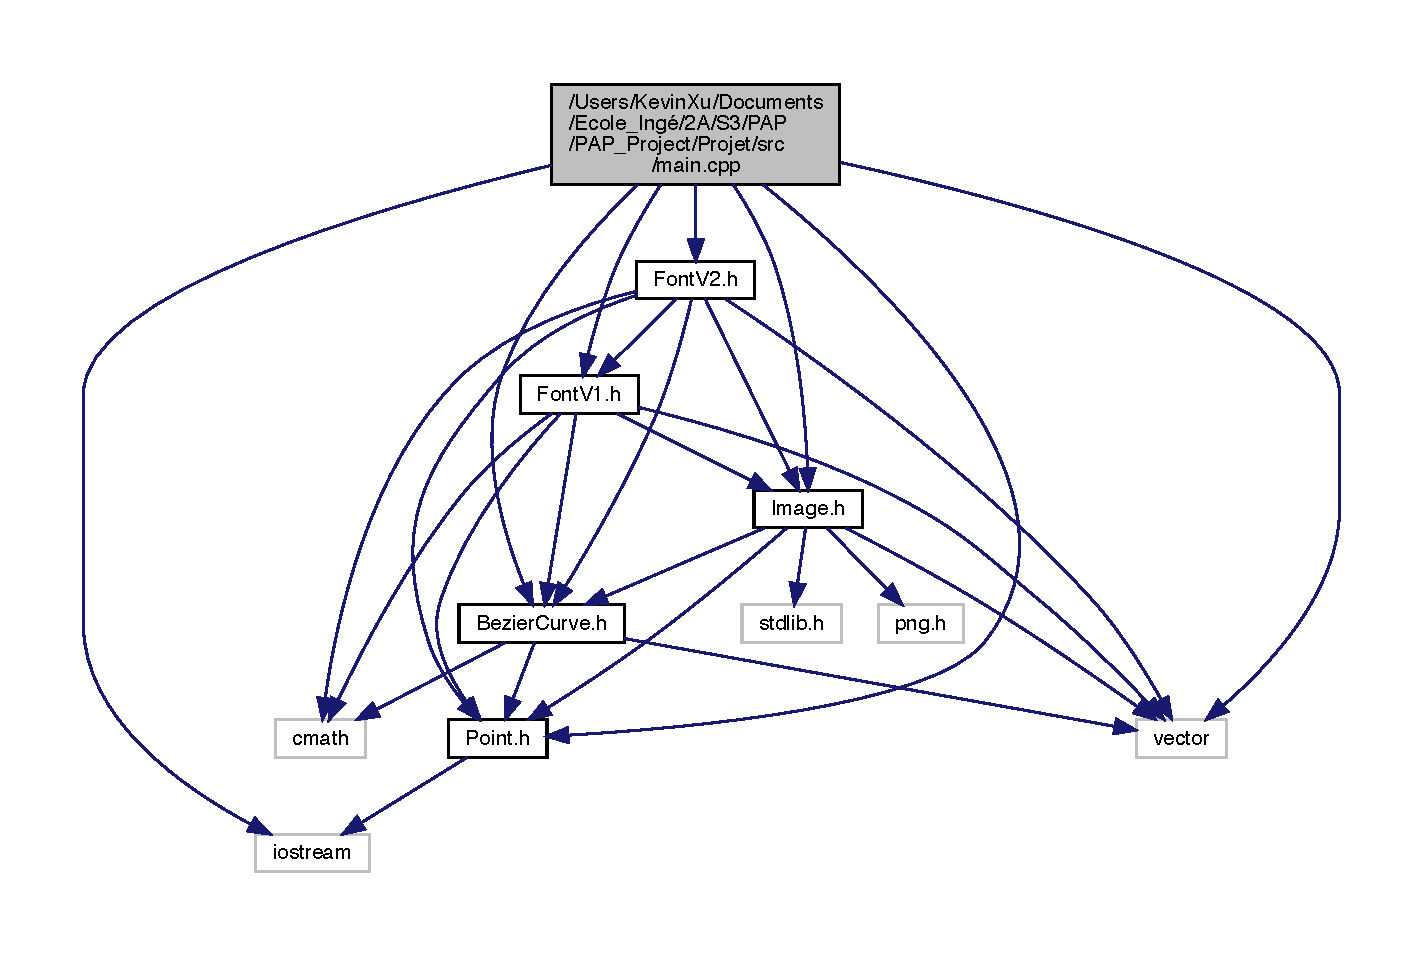
\includegraphics[width=350pt]{main_8cpp__incl}
\end{center}
\end{figure}
\subsection*{Functions}
\begin{DoxyCompactItemize}
\item 
int \mbox{\hyperlink{main_8cpp_ae66f6b31b5ad750f1fe042a706a4e3d4}{main}} ()
\end{DoxyCompactItemize}


\subsection{Function Documentation}
\mbox{\Hypertarget{main_8cpp_ae66f6b31b5ad750f1fe042a706a4e3d4}\label{main_8cpp_ae66f6b31b5ad750f1fe042a706a4e3d4}} 
\index{main.\+cpp@{main.\+cpp}!main@{main}}
\index{main@{main}!main.\+cpp@{main.\+cpp}}
\subsubsection{\texorpdfstring{main()}{main()}}
{\footnotesize\ttfamily int main (\begin{DoxyParamCaption}{ }\end{DoxyParamCaption})}


\begin{DoxyCode}
10            \{
11     \textcolor{comment}{// FONTV1}
12     \textcolor{comment}{// char fileName1A[] = "./FontV1/FontV1\_A.png";}
13     \textcolor{comment}{// FontV1 L1A(fileName1A);}
14     \textcolor{comment}{// L1A.A();}
15     \textcolor{comment}{// L1A.finishLetter();}
16 
17     \textcolor{comment}{// char fileName1B[] = "./FontV1/FontV1\_B.png";}
18     \textcolor{comment}{// FontV1 L1B(fileName1B);}
19     \textcolor{comment}{// L1B.B();}
20     \textcolor{comment}{// L1B.finishLetter();}
21 
22     \textcolor{comment}{// char fileName1C[] = "./FontV1/FontV1\_C.png";}
23     \textcolor{comment}{// FontV1 L1C(fileName1C);}
24     \textcolor{comment}{// L1C.C();}
25     \textcolor{comment}{// L1C.finishLetter();}
26 
27     \textcolor{comment}{// char fileName1D[] = "./FontV1/FontV1\_D.png";}
28     \textcolor{comment}{// FontV1 L1D(fileName1D);}
29     \textcolor{comment}{// L1D.D();}
30     \textcolor{comment}{// L1D.finishLetter();}
31 
32     \textcolor{comment}{// char fileName1E[] = "./FontV1/FontV1\_E.png";}
33     \textcolor{comment}{// FontV1 L1E(fileName1E);}
34     \textcolor{comment}{// L1E.E();}
35     \textcolor{comment}{// L1E.finishLetter();}
36 
37     \textcolor{comment}{// char fileName1F[] = "./FontV1/FontV1\_F.png";}
38     \textcolor{comment}{// FontV1 L1F(fileName1F);}
39     \textcolor{comment}{// L1F.F();}
40     \textcolor{comment}{// L1F.finishLetter();}
41 
42     \textcolor{comment}{// char fileName1G[] = "./FontV1/FontV1\_G.png";}
43     \textcolor{comment}{// FontV1 L1G(fileName1G);}
44     \textcolor{comment}{// L1G.G();}
45     \textcolor{comment}{// L1G.finishLetter();}
46 
47     \textcolor{comment}{// char fileName1H[] = "./FontV1/FontV1\_H.png";}
48     \textcolor{comment}{// FontV1 L1H(fileName1H);}
49     \textcolor{comment}{// L1H.H();}
50     \textcolor{comment}{// L1H.finishLetter();}
51 
52     \textcolor{comment}{// char fileName1I[] = "./FontV1/FontV1\_I.png";}
53     \textcolor{comment}{// FontV1 L1I(fileName1I);}
54     \textcolor{comment}{// L1I.I();}
55     \textcolor{comment}{// L1I.finishLetter();}
56 
57     \textcolor{comment}{// char fileName1J[] = "./FontV1/FontV1\_J.png";}
58     \textcolor{comment}{// FontV1 L1J(fileName1J);}
59     \textcolor{comment}{// L1J.J();}
60     \textcolor{comment}{// L1J.finishLetter();}
61 
62     \textcolor{comment}{// char fileName1K[] = "./FontV1/FontV1\_K.png";}
63     \textcolor{comment}{// FontV1 L1K(fileName1K);}
64     \textcolor{comment}{// L1K.K();}
65     \textcolor{comment}{// L1K.finishLetter();}
66 
67     \textcolor{comment}{// char fileName1L[] = "./FontV1/FontV1\_L.png";}
68     \textcolor{comment}{// FontV1 L1L(fileName1L);}
69     \textcolor{comment}{// L1L.L();}
70     \textcolor{comment}{// L1L.finishLetter();}
71 
72     \textcolor{comment}{// char fileName1M[] = "./FontV1/FontV1\_M.png";}
73     \textcolor{comment}{// FontV1 L1M(fileName1M);}
74     \textcolor{comment}{// L1M.M();}
75     \textcolor{comment}{// L1M.finishLetter();}
76 
77     \textcolor{comment}{// char fileName1N[] = "./FontV1/FontV1\_N.png";}
78     \textcolor{comment}{// FontV1 L1N(fileName1N);}
79     \textcolor{comment}{// L1N.N();}
80     \textcolor{comment}{// L1N.finishLetter();}
81 
82     \textcolor{comment}{// char fileName1O[] = "./FontV1/FontV1\_O.png";}
83     \textcolor{comment}{// FontV1 L1O(fileName1O);}
84     \textcolor{comment}{// L1O.O();}
85     \textcolor{comment}{// L1O.finishLetter();}
86 
87     \textcolor{comment}{// char fileName1P[] = "./FontV1/FontV1\_P.png";}
88     \textcolor{comment}{// FontV1 L1P(fileName1P);}
89     \textcolor{comment}{// L1P.P();}
90     \textcolor{comment}{// L1P.finishLetter();}
91 
92     \textcolor{comment}{// char fileName1Q[] = "./FontV1/FontV1\_Q.png";}
93     \textcolor{comment}{// FontV1 L1Q(fileName1Q);}
94     \textcolor{comment}{// L1Q.Q();}
95     \textcolor{comment}{// L1Q.finishLetter();}
96 
97     \textcolor{comment}{// char fileName1R[] = "./FontV1/FontV1\_R.png";}
98     \textcolor{comment}{// FontV1 L1R(fileName1R);}
99     \textcolor{comment}{// L1R.R();}
100     \textcolor{comment}{// L1R.finishLetter();}
101 
102     \textcolor{comment}{// char fileName1S[] = "./FontV1/FontV1\_S.png";}
103     \textcolor{comment}{// FontV1 L1S(fileName1S);}
104     \textcolor{comment}{// L1S.S();}
105     \textcolor{comment}{// L1S.finishLetter();}
106 
107     \textcolor{comment}{// char fileName1T[] = "./FontV1/FontV1\_T.png";}
108     \textcolor{comment}{// FontV1 L1T(fileName1T);}
109     \textcolor{comment}{// L1T.T();}
110     \textcolor{comment}{// L1T.finishLetter();}
111 
112     \textcolor{comment}{// char fileName1U[] = "./FontV1/FontV1\_U.png";}
113     \textcolor{comment}{// FontV1 L1U(fileName1U);}
114     \textcolor{comment}{// L1U.U();}
115     \textcolor{comment}{// L1U.finishLetter();}
116 
117     \textcolor{comment}{// char fileName1V[] = "./FontV1/FontV1\_V.png";}
118     \textcolor{comment}{// FontV1 L1V(fileName1V);}
119     \textcolor{comment}{// L1V.V();}
120     \textcolor{comment}{// L1V.finishLetter();}
121 
122     \textcolor{comment}{// char fileName1W[] = "./FontV1/FontV1\_W.png";}
123     \textcolor{comment}{// FontV1 L1W(fileName1W);}
124     \textcolor{comment}{// L1W.W();}
125     \textcolor{comment}{// L1W.finishLetter();}
126 
127     \textcolor{comment}{// char fileName1X[] = "./FontV1/FontV1\_X.png";}
128     \textcolor{comment}{// FontV1 L1X(fileName1X);}
129     \textcolor{comment}{// L1X.X();}
130     \textcolor{comment}{// L1X.finishLetter();}
131 
132     \textcolor{comment}{// char fileName1Y[] = "./FontV1/FontV1\_Y.png";}
133     \textcolor{comment}{// FontV1 L1Y(fileName1Y);}
134     \textcolor{comment}{// L1Y.Y();}
135     \textcolor{comment}{// L1Y.finishLetter();}
136 
137     \textcolor{comment}{// char fileName1Z[] = "./FontV1/FontV1\_Z.png";}
138     \textcolor{comment}{// FontV1 L1Z(fileName1Z);}
139     \textcolor{comment}{// L1Z.Z();}
140     \textcolor{comment}{// L1Z.finishLetter();}
141 
142 
143 
144     \textcolor{comment}{// FONTV2}
145     \textcolor{comment}{// char fileName2A[] = "./FontV2/FontV2\_A.png";}
146     \textcolor{comment}{// FontV2 L2A(fileName2A);}
147     \textcolor{comment}{// L2A.A();}
148     \textcolor{comment}{// L2A.finishLetter();}
149 
150     \textcolor{comment}{// char fileName2B[] = "./FontV2/FontV2\_B.png";}
151     \textcolor{comment}{// FontV2 L2B(fileName2B);}
152     \textcolor{comment}{// L2B.B();}
153     \textcolor{comment}{// L2B.finishLetter();}
154 
155     \textcolor{comment}{// char fileName2C[] = "./FontV2/FontV2\_C.png";}
156     \textcolor{comment}{// FontV2 L2C(fileName2C);}
157     \textcolor{comment}{// L2C.C();}
158     \textcolor{comment}{// L2C.finishLetter();}
159 
160     \textcolor{comment}{// char fileName2D[] = "./FontV2/FontV2\_D.png";}
161     \textcolor{comment}{// FontV2 L2D(fileName2D);}
162     \textcolor{comment}{// L2D.D();}
163     \textcolor{comment}{// L2D.finishLetter();}
164 
165     \textcolor{comment}{// char fileName2E[] = "./FontV2/FontV2\_E.png";}
166     \textcolor{comment}{// FontV2 L2E(fileName2E);}
167     \textcolor{comment}{// L2E.E();}
168     \textcolor{comment}{// L2E.finishLetter();}
169 
170     \textcolor{comment}{// char fileName2F[] = "./FontV2/FontV2\_F.png";}
171     \textcolor{comment}{// FontV2 L2F(fileName2F);}
172     \textcolor{comment}{// L2F.F();}
173     \textcolor{comment}{// L2F.finishLetter();}
174 
175     \textcolor{comment}{// char fileName2G[] = "./FontV2/FontV2\_G.png";}
176     \textcolor{comment}{// FontV2 L2G(fileName2G);}
177     \textcolor{comment}{// L2G.G();}
178     \textcolor{comment}{// L2G.finishLetter();}
179 
180     \textcolor{comment}{// char fileName2H[] = "./FontV2/FontV2\_H.png";}
181     \textcolor{comment}{// FontV2 L2H(fileName2H);}
182     \textcolor{comment}{// L2H.H();}
183     \textcolor{comment}{// L2H.finishLetter();}
184 
185     \textcolor{comment}{// char fileName2I[] = "./FontV2/FontV2\_I.png";}
186     \textcolor{comment}{// FontV2 L2I(fileName2I);}
187     \textcolor{comment}{// L2I.I();}
188     \textcolor{comment}{// L2I.finishLetter();}
189 
190     \textcolor{comment}{// char fileName2J[] = "./FontV2/FontV2\_J.png";}
191     \textcolor{comment}{// FontV2 L2J(fileName2J);}
192     \textcolor{comment}{// L2J.J();}
193     \textcolor{comment}{// L2J.finishLetter();}
194 
195     \textcolor{comment}{// char fileName2K[] = "./FontV2/FontV2\_K.png";}
196     \textcolor{comment}{// FontV2 L2K(fileName2K);}
197     \textcolor{comment}{// L2K.K();}
198     \textcolor{comment}{// L2K.finishLetter();}
199 
200     \textcolor{comment}{// char fileName2L[] = "./FontV2/FontV2\_L.png";}
201     \textcolor{comment}{// FontV2 L2L(fileName2L);}
202     \textcolor{comment}{// L2L.L();}
203     \textcolor{comment}{// L2L.finishLetter();}
204 
205     \textcolor{comment}{// char fileName2M[] = "./FontV2/FontV2\_M.png";}
206     \textcolor{comment}{// FontV2 L2M(fileName2M);}
207     \textcolor{comment}{// L2M.M();}
208     \textcolor{comment}{// L2M.finishLetter();}
209 
210     \textcolor{comment}{// char fileName2N[] = "./FontV2/FontV2\_N.png";}
211     \textcolor{comment}{// FontV2 L2N(fileName2N);}
212     \textcolor{comment}{// L2N.N();}
213     \textcolor{comment}{// L2N.finishLetter();}
214 
215     \textcolor{comment}{// char fileName2O[] = "./FontV2/FontV2\_O.png";}
216     \textcolor{comment}{// FontV2 L2O(fileName2O);}
217     \textcolor{comment}{// L2O.O();}
218     \textcolor{comment}{// L2O.finishLetter();}
219 
220     \textcolor{comment}{// char fileName2P[] = "./FontV2/FontV2\_P.png";}
221     \textcolor{comment}{// FontV2 L2P(fileName2P);}
222     \textcolor{comment}{// L2P.P();}
223     \textcolor{comment}{// L2P.finishLetter();}
224 
225     \textcolor{comment}{// char fileName2Q[] = "./FontV2/FontV2\_Q.png";}
226     \textcolor{comment}{// FontV2 L2Q(fileName2Q);}
227     \textcolor{comment}{// L2Q.Q();}
228     \textcolor{comment}{// L2Q.finishLetter();}
229 
230     \textcolor{comment}{// char fileName2R[] = "./FontV2/FontV2\_R.png";}
231     \textcolor{comment}{// FontV2 L2R(fileName2R);}
232     \textcolor{comment}{// L2R.R();}
233     \textcolor{comment}{// L2R.finishLetter();}
234 
235     \textcolor{comment}{// char fileName2S[] = "./FontV2/FontV2\_S.png";}
236     \textcolor{comment}{// FontV2 L2S(fileName2S);}
237     \textcolor{comment}{// L2S.S();}
238     \textcolor{comment}{// L2S.finishLetter();}
239 
240     \textcolor{comment}{// char fileName2T[] = "./FontV2/FontV2\_T.png";}
241     \textcolor{comment}{// FontV2 L2T(fileName2T);}
242     \textcolor{comment}{// L2T.T();}
243     \textcolor{comment}{// L2T.finishLetter();}
244 
245     \textcolor{comment}{// char fileName2U[] = "./FontV2/FontV2\_U.png";}
246     \textcolor{comment}{// FontV2 L2U(fileName2U);}
247     \textcolor{comment}{// L2U.U();}
248     \textcolor{comment}{// L2U.finishLetter();}
249 
250     \textcolor{comment}{// char fileName2V[] = "./FontV2/FontV2\_V.png";}
251     \textcolor{comment}{// FontV2 L2V(fileName2V);}
252     \textcolor{comment}{// L2V.V();}
253     \textcolor{comment}{// L2V.finishLetter();}
254 
255     \textcolor{comment}{// char fileName2W[] = "./FontV2/FontV2\_W.png";}
256     \textcolor{comment}{// FontV2 L2W(fileName2W);}
257     \textcolor{comment}{// L2W.W();}
258     \textcolor{comment}{// L2W.finishLetter();}
259 
260     \textcolor{comment}{// char fileName2X[] = "./FontV2/FontV2\_X.png";}
261     \textcolor{comment}{// FontV2 L2X(fileName2X);}
262     \textcolor{comment}{// L2X.X();}
263     \textcolor{comment}{// L2X.finishLetter();}
264 
265     \textcolor{comment}{// char fileName2Y[] = "./FontV2/FontV2\_Y.png";}
266     \textcolor{comment}{// FontV2 L2Y(fileName2Y);}
267     \textcolor{comment}{// L2Y.Y();}
268     \textcolor{comment}{// L2Y.finishLetter();}
269 
270     \textcolor{comment}{// char fileName2Z[] = "./FontV2/FontV2\_Z.png";}
271     \textcolor{comment}{// FontV2 L2Z(fileName2Z);}
272     \textcolor{comment}{// L2Z.Z();}
273     \textcolor{comment}{// L2Z.finishLetter();}
274 
275 
276     \textcolor{comment}{// FONTV3}
277     \textcolor{comment}{// char fileName3A[] = "./FontV3/FontV3\_A.png";}
278  \textcolor{comment}{//    FontV3 L3A(fileName3A);}
279  \textcolor{comment}{//    L3A.A();}
280  \textcolor{comment}{//    L3A.finishLetter();}
281 
282  \textcolor{comment}{//    char fileName3B[] = "./FontV3/FontV3\_B.png";}
283  \textcolor{comment}{//    FontV3 L3B(fileName3B);}
284  \textcolor{comment}{//    L3B.B();}
285  \textcolor{comment}{//    L3B.finishLetter();}
286 
287  \textcolor{comment}{//    char fileName3C[] = "./FontV3/FontV3\_C.png";}
288  \textcolor{comment}{//    FontV3 L3C(fileName3C);}
289  \textcolor{comment}{//    L3C.C();}
290  \textcolor{comment}{//    L3C.finishLetter();}
291 
292  \textcolor{comment}{//    char fileName3D[] = "./FontV3/FontV3\_D.png";}
293  \textcolor{comment}{//    FontV3 L3D(fileName3D);}
294  \textcolor{comment}{//    L3D.D();}
295  \textcolor{comment}{//    L3D.finishLetter();}
296 
297  \textcolor{comment}{//    char fileName3E[] = "./FontV3/FontV3\_E.png";}
298  \textcolor{comment}{//    FontV3 L3E(fileName3E);}
299  \textcolor{comment}{//    L3E.E();}
300  \textcolor{comment}{//    L3E.finishLetter();}
301 
302  \textcolor{comment}{//    char fileName3F[] = "./FontV3/FontV3\_F.png";}
303  \textcolor{comment}{//    FontV3 L3F(fileName3F);}
304  \textcolor{comment}{//    L3F.F();}
305  \textcolor{comment}{//    L3F.finishLetter();}
306 
307  \textcolor{comment}{//    char fileName3G[] = "./FontV3/FontV3\_G.png";}
308  \textcolor{comment}{//    FontV3 L3G(fileName3G);}
309  \textcolor{comment}{//    L3G.G();}
310  \textcolor{comment}{//    L3G.finishLetter();}
311 
312  \textcolor{comment}{//    char fileName3H[] = "./FontV3/FontV3\_H.png";}
313  \textcolor{comment}{//    FontV3 L3H(fileName3H);}
314  \textcolor{comment}{//    L3H.H();}
315  \textcolor{comment}{//    L3H.finishLetter();}
316 
317  \textcolor{comment}{//    char fileName3I[] = "./FontV3/FontV3\_I.png";}
318  \textcolor{comment}{//    FontV3 L3I(fileName3I);}
319  \textcolor{comment}{//    L3I.I();}
320  \textcolor{comment}{//    L3I.finishLetter();}
321 
322  \textcolor{comment}{//    char fileName3J[] = "./FontV3/FontV3\_J.png";}
323  \textcolor{comment}{//    FontV3 L3J(fileName3J);}
324  \textcolor{comment}{//    L3J.J();}
325  \textcolor{comment}{//    L3J.finishLetter();}
326 
327  \textcolor{comment}{//    char fileName3K[] = "./FontV3/FontV3\_K.png";}
328  \textcolor{comment}{//    FontV3 L3K(fileName3K);}
329  \textcolor{comment}{//    L3K.K();}
330  \textcolor{comment}{//    L3K.finishLetter();}
331 
332  \textcolor{comment}{//    char fileName3L[] = "./FontV3/FontV3\_L.png";}
333  \textcolor{comment}{//    FontV3 L3L(fileName3L);}
334  \textcolor{comment}{//    L3L.L();}
335  \textcolor{comment}{//    L3L.finishLetter();}
336 
337  \textcolor{comment}{//    char fileName3M[] = "./FontV3/FontV3\_M.png";}
338  \textcolor{comment}{//    FontV3 L3M(fileName3M);}
339  \textcolor{comment}{//    L3M.M();}
340  \textcolor{comment}{//    L3M.finishLetter();}
341 
342  \textcolor{comment}{//    char fileName3N[] = "./FontV3/FontV3\_N.png";}
343  \textcolor{comment}{//    FontV3 L3N(fileName3N);}
344  \textcolor{comment}{//    L3N.N();}
345  \textcolor{comment}{//    L3N.finishLetter();}
346 
347  \textcolor{comment}{//    char fileName3O[] = "./FontV3/FontV3\_O.png";}
348  \textcolor{comment}{//    FontV3 L3O(fileName3O);}
349  \textcolor{comment}{//    L3O.O();}
350  \textcolor{comment}{//    L3O.finishLetter();}
351 
352  \textcolor{comment}{//    char fileName3P[] = "./FontV3/FontV3\_P.png";}
353  \textcolor{comment}{//    FontV3 L3P(fileName3P);}
354  \textcolor{comment}{//    L3P.P();}
355  \textcolor{comment}{//    L3P.finishLetter();}
356 
357  \textcolor{comment}{//    char fileName3Q[] = "./FontV3/FontV3\_Q.png";}
358  \textcolor{comment}{//    FontV3 L3Q(fileName3Q);}
359  \textcolor{comment}{//    L3Q.Q();}
360  \textcolor{comment}{//    L3Q.finishLetter();}
361 
362  \textcolor{comment}{//    char fileName3R[] = "./FontV3/FontV3\_R.png";}
363  \textcolor{comment}{//    FontV3 L3R(fileName3R);}
364  \textcolor{comment}{//    L3R.R();}
365  \textcolor{comment}{//    L3R.finishLetter();}
366 
367     \textcolor{keywordtype}{char} fileName3S[] = \textcolor{stringliteral}{"./FontV3/FontV3\_S.png"};
368     \mbox{\hyperlink{class_font_v3}{FontV3}} L3S(fileName3S);
369     L3S.S();
370     L3S.finishLetter();
371 
372  \textcolor{comment}{//    char fileName3T[] = "./FontV3/FontV3\_T.png";}
373  \textcolor{comment}{//    FontV3 L3T(fileName3T);}
374  \textcolor{comment}{//    L3T.T();}
375  \textcolor{comment}{//    L3T.finishLetter();}
376 
377  \textcolor{comment}{//    char fileName3U[] = "./FontV3/FontV3\_U.png";}
378  \textcolor{comment}{//    FontV3 L3U(fileName3U);}
379  \textcolor{comment}{//    L3U.U();}
380  \textcolor{comment}{//    L3U.finishLetter();}
381 
382  \textcolor{comment}{//    char fileName3V[] = "./FontV3/FontV3\_V.png";}
383  \textcolor{comment}{//    FontV3 L3V(fileName3V);}
384  \textcolor{comment}{//    L3V.V();}
385  \textcolor{comment}{//    L3V.finishLetter();}
386 
387  \textcolor{comment}{//    char fileName3W[] = "./FontV3/FontV3\_W.png";}
388  \textcolor{comment}{//    FontV3 L3W(fileName3W);}
389  \textcolor{comment}{//    L3W.W();}
390  \textcolor{comment}{//    L3W.finishLetter();}
391 
392  \textcolor{comment}{//    char fileName3X[] = "./FontV3/FontV3\_X.png";}
393  \textcolor{comment}{//    FontV3 L3X(fileName3X);}
394  \textcolor{comment}{//    L3X.X();}
395  \textcolor{comment}{//    L3X.finishLetter();}
396 
397  \textcolor{comment}{//    char fileName3Y[] = "./FontV3/FontV3\_Y.png";}
398  \textcolor{comment}{//    FontV3 L3Y(fileName3Y);}
399  \textcolor{comment}{//    L3Y.Y();}
400  \textcolor{comment}{//    L3Y.finishLetter();}
401 
402  \textcolor{comment}{//    char fileName3Z[] = "./FontV3/FontV3\_Z.png";}
403  \textcolor{comment}{//    FontV3 L3Z(fileName3Z);}
404  \textcolor{comment}{//    L3Z.Z();}
405  \textcolor{comment}{//    L3Z.finishLetter();}
406 
407     \textcolor{keywordflow}{return} 0;
408 \}
\end{DoxyCode}

\hypertarget{main_b_e_z_i_e_rplusieurs_points_8cpp}{}\section{/\+Users/\+Kevin\+Xu/\+Documents/\+Ecole\+\_\+\+Ingé/2\+A/\+S3/\+P\+A\+P/\+P\+A\+P\+\_\+\+Project/\+Projet/src/main\+B\+E\+Z\+I\+E\+Rplusieurs\+Points.cpp File Reference}
\label{main_b_e_z_i_e_rplusieurs_points_8cpp}\index{/\+Users/\+Kevin\+Xu/\+Documents/\+Ecole\+\_\+\+Ingé/2\+A/\+S3/\+P\+A\+P/\+P\+A\+P\+\_\+\+Project/\+Projet/src/main\+B\+E\+Z\+I\+E\+Rplusieurs\+Points.\+cpp@{/\+Users/\+Kevin\+Xu/\+Documents/\+Ecole\+\_\+\+Ingé/2\+A/\+S3/\+P\+A\+P/\+P\+A\+P\+\_\+\+Project/\+Projet/src/main\+B\+E\+Z\+I\+E\+Rplusieurs\+Points.\+cpp}}
{\ttfamily \#include $<$iostream$>$}\newline
{\ttfamily \#include \char`\"{}Point.\+h\char`\"{}}\newline
{\ttfamily \#include \char`\"{}Image.\+h\char`\"{}}\newline
{\ttfamily \#include \char`\"{}Line.\+h\char`\"{}}\newline
{\ttfamily \#include $<$vector$>$}\newline
Include dependency graph for main\+B\+E\+Z\+I\+E\+Rplusieurs\+Points.\+cpp\+:
\nopagebreak
\begin{figure}[H]
\begin{center}
\leavevmode
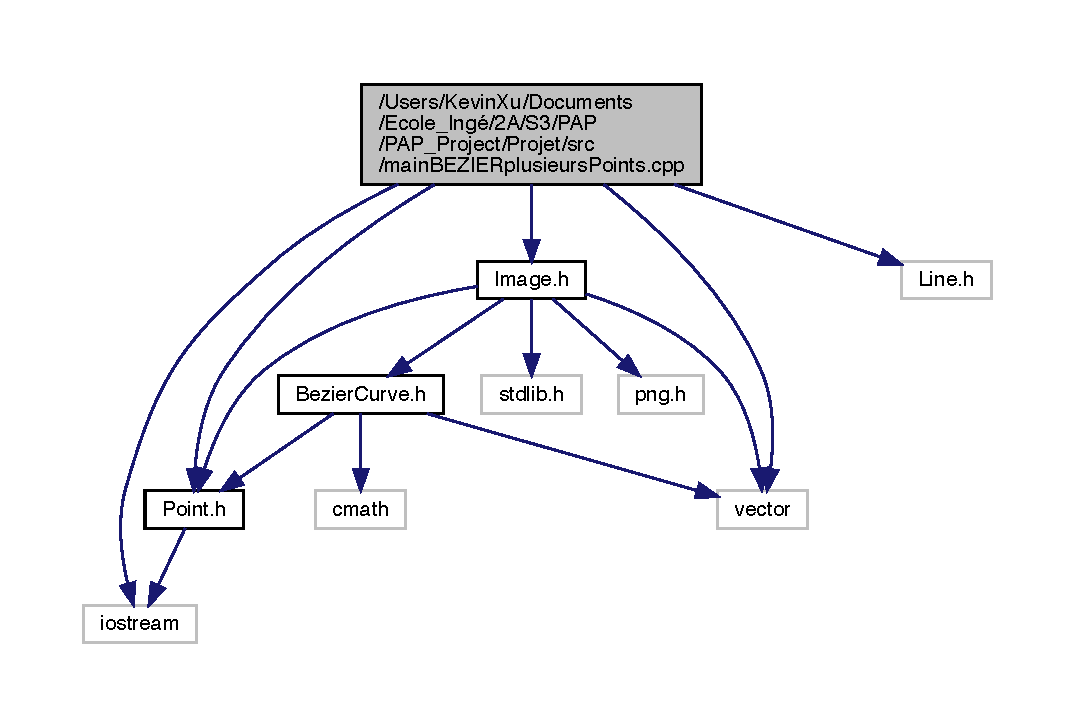
\includegraphics[width=350pt]{main_b_e_z_i_e_rplusieurs_points_8cpp__incl}
\end{center}
\end{figure}
\subsection*{Functions}
\begin{DoxyCompactItemize}
\item 
\mbox{\hyperlink{class_point}{Point}} \mbox{\hyperlink{main_b_e_z_i_e_rplusieurs_points_8cpp_af9d5a929caa85aecb7951dcb95dda799}{get\+C\+J\+Point}} (int r, int i, double t, std\+::vector$<$ \mbox{\hyperlink{class_point}{Point}} $>$ points)
\item 
std\+::vector$<$ \mbox{\hyperlink{class_point}{Point}} $>$ \mbox{\hyperlink{main_b_e_z_i_e_rplusieurs_points_8cpp_aecbd307881401b6d8aaa05a4331769f2}{draw\+CJ}} (std\+::vector$<$ \mbox{\hyperlink{class_point}{Point}} $>$ points)
\item 
int \mbox{\hyperlink{main_b_e_z_i_e_rplusieurs_points_8cpp_ae66f6b31b5ad750f1fe042a706a4e3d4}{main}} ()
\end{DoxyCompactItemize}


\subsection{Function Documentation}
\mbox{\Hypertarget{main_b_e_z_i_e_rplusieurs_points_8cpp_aecbd307881401b6d8aaa05a4331769f2}\label{main_b_e_z_i_e_rplusieurs_points_8cpp_aecbd307881401b6d8aaa05a4331769f2}} 
\index{main\+B\+E\+Z\+I\+E\+Rplusieurs\+Points.\+cpp@{main\+B\+E\+Z\+I\+E\+Rplusieurs\+Points.\+cpp}!draw\+CJ@{draw\+CJ}}
\index{draw\+CJ@{draw\+CJ}!main\+B\+E\+Z\+I\+E\+Rplusieurs\+Points.\+cpp@{main\+B\+E\+Z\+I\+E\+Rplusieurs\+Points.\+cpp}}
\subsubsection{\texorpdfstring{draw\+C\+J()}{drawCJ()}}
{\footnotesize\ttfamily std\+::vector$<$\mbox{\hyperlink{class_point}{Point}}$>$ draw\+CJ (\begin{DoxyParamCaption}\item[{std\+::vector$<$ \mbox{\hyperlink{class_point}{Point}} $>$}]{points }\end{DoxyParamCaption})}


\begin{DoxyCode}
24                                                  \{
25     std::vector<Point> res;
26     \textcolor{keywordflow}{for} (\textcolor{keywordtype}{double} t = 0.0; t <= 1; t+=0.00001) \{
27         \mbox{\hyperlink{class_point}{Point}} P = \mbox{\hyperlink{main_b_e_z_i_e_rplusieurs_points_8cpp_af9d5a929caa85aecb7951dcb95dda799}{getCJPoint}}(points.size() - 1, 0, t, points);
28         res.push\_back(P);
29     \}
30     \textcolor{keywordflow}{return} res;
31 \}
\end{DoxyCode}
\mbox{\Hypertarget{main_b_e_z_i_e_rplusieurs_points_8cpp_af9d5a929caa85aecb7951dcb95dda799}\label{main_b_e_z_i_e_rplusieurs_points_8cpp_af9d5a929caa85aecb7951dcb95dda799}} 
\index{main\+B\+E\+Z\+I\+E\+Rplusieurs\+Points.\+cpp@{main\+B\+E\+Z\+I\+E\+Rplusieurs\+Points.\+cpp}!get\+C\+J\+Point@{get\+C\+J\+Point}}
\index{get\+C\+J\+Point@{get\+C\+J\+Point}!main\+B\+E\+Z\+I\+E\+Rplusieurs\+Points.\+cpp@{main\+B\+E\+Z\+I\+E\+Rplusieurs\+Points.\+cpp}}
\subsubsection{\texorpdfstring{get\+C\+J\+Point()}{getCJPoint()}}
{\footnotesize\ttfamily \mbox{\hyperlink{class_point}{Point}} get\+C\+J\+Point (\begin{DoxyParamCaption}\item[{int}]{r,  }\item[{int}]{i,  }\item[{double}]{t,  }\item[{std\+::vector$<$ \mbox{\hyperlink{class_point}{Point}} $>$}]{points }\end{DoxyParamCaption})}


\begin{DoxyCode}
17                                                                   \{
18     \textcolor{keywordflow}{if} (r == 0) \textcolor{keywordflow}{return} points[i];
19     \mbox{\hyperlink{class_point}{Point}} P1 = \mbox{\hyperlink{main_b_e_z_i_e_rplusieurs_points_8cpp_af9d5a929caa85aecb7951dcb95dda799}{getCJPoint}}(r-1, i, t, points);
20     \mbox{\hyperlink{class_point}{Point}} P2 = \mbox{\hyperlink{main_b_e_z_i_e_rplusieurs_points_8cpp_af9d5a929caa85aecb7951dcb95dda799}{getCJPoint}}(r-1, i+1, t, points);
21     \textcolor{keywordflow}{return} \mbox{\hyperlink{class_point}{Point}}(\textcolor{keywordtype}{int}((1-t) * P1.\mbox{\hyperlink{class_point_ac9d5859db121c7d1b89ca89266dca0a3}{getX}}() + t * P2.\mbox{\hyperlink{class_point_ac9d5859db121c7d1b89ca89266dca0a3}{getX}}()), \textcolor{keywordtype}{int}((1 - t) * P1.
      \mbox{\hyperlink{class_point_a86d10ff46e08462c45b15a8c7ef62d61}{getY}}() + t * P2.\mbox{\hyperlink{class_point_a86d10ff46e08462c45b15a8c7ef62d61}{getY}}()));
22 \}
\end{DoxyCode}
\mbox{\Hypertarget{main_b_e_z_i_e_rplusieurs_points_8cpp_ae66f6b31b5ad750f1fe042a706a4e3d4}\label{main_b_e_z_i_e_rplusieurs_points_8cpp_ae66f6b31b5ad750f1fe042a706a4e3d4}} 
\index{main\+B\+E\+Z\+I\+E\+Rplusieurs\+Points.\+cpp@{main\+B\+E\+Z\+I\+E\+Rplusieurs\+Points.\+cpp}!main@{main}}
\index{main@{main}!main\+B\+E\+Z\+I\+E\+Rplusieurs\+Points.\+cpp@{main\+B\+E\+Z\+I\+E\+Rplusieurs\+Points.\+cpp}}
\subsubsection{\texorpdfstring{main()}{main()}}
{\footnotesize\ttfamily int main (\begin{DoxyParamCaption}{ }\end{DoxyParamCaption})}


\begin{DoxyCode}
34            \{
35     std::cout << \textcolor{stringliteral}{"!!!Hello World!!!"} << std::endl;
36 
37     \mbox{\hyperlink{class_point}{Point}} P(1, 2);
38     std::cout << P << std::endl;
39 
40     \textcolor{keywordtype}{char} fileName[] = \textcolor{stringliteral}{"img.png"};
41     \mbox{\hyperlink{class_image}{Image}} img(fileName, 5000, 5000);
42 
43     \textcolor{comment}{// Modif pixels}
44     \textcolor{comment}{// png\_bytep* pixels = img.getPixels();}
45     \textcolor{comment}{// for(int y = 0; y < 10000; y++) \{}
46     \textcolor{comment}{//     png\_bytep row = pixels[y];}
47     \textcolor{comment}{//     for(int x = 0; x < 1000; x++) \{}
48     \textcolor{comment}{//      png\_bytep px = \&(row[x * 3]);}
49     \textcolor{comment}{//      px[0] = 0;}
50     \textcolor{comment}{//      px[1] = 255;}
51     \textcolor{comment}{//      px[2] = 0;}
52     \textcolor{comment}{//     \}}
53  \textcolor{comment}{//     \}}
54 
55 
56     \textcolor{comment}{// Test horizontal line }
57     \mbox{\hyperlink{class_point}{Point}} P1(2500, 10);
58     \mbox{\hyperlink{class_point}{Point}} P2(2500, 4500);
59     \textcolor{comment}{// Line L1(P1, P2);}
60    \textcolor{comment}{//  std::cout << L1 << std::endl;}
61    \textcolor{comment}{//  img.drawStraightLine(L1);}
62 
63     \textcolor{comment}{// Test horizontal line }
64     \mbox{\hyperlink{class_point}{Point}} P3(5, 4500);
65     \mbox{\hyperlink{class_point}{Point}} P4(5000, 4500);
66     Line L2(P3, P4);
67     std::cout << L2 << std::endl;
68     img.drawStraightLine(L2);
69 
70     \mbox{\hyperlink{class_point}{Point}} P5(5, 3000);
71     \mbox{\hyperlink{class_point}{Point}} P6(5000, 4500);
72     Line L3(P5, P6);
73     std::cout << L3 << std::endl;
74     img.draw(L3);
75 
76 
77     \textcolor{comment}{// draw Point}
78     \mbox{\hyperlink{class_point}{Point}} P7(1, 1);
79     img.draw(P7); 
80 
81     \textcolor{comment}{// draw curve}
82     \mbox{\hyperlink{class_point}{Point}} P10(1, 2500);
83     \mbox{\hyperlink{class_point}{Point}} P11(1400, 1000);
84     \mbox{\hyperlink{class_point}{Point}} P12(2500, 2600);
85     \mbox{\hyperlink{class_point}{Point}} P13(4888, 500);
86 
87     std::vector<Point> points;
88     points.push\_back(P10);
89     points.push\_back(P11);
90     points.push\_back(P12);
91 
92     std::vector<Point> result = \mbox{\hyperlink{main_b_e_z_i_e_rplusieurs_points_8cpp_aecbd307881401b6d8aaa05a4331769f2}{drawCJ}}(points);
93     \textcolor{keywordflow}{for} (std::vector<Point>::iterator it = result.begin(); it != result.end(); it++) \{
94         img.draw(*it);
95     \}
96 
97 
98     std::vector<Point> points2;
99     points2.push\_back(P1);
100     points2.push\_back(P2);
101 
102     std::vector<Point> result2 = \mbox{\hyperlink{main_b_e_z_i_e_rplusieurs_points_8cpp_aecbd307881401b6d8aaa05a4331769f2}{drawCJ}}(points2);
103     \textcolor{keywordflow}{for} (std::vector<Point>::iterator it = result2.begin(); it != result2.end(); it++) \{
104         img.draw(*it);
105     \}
106 
107     \textcolor{comment}{//img.setPixels(pixels);}
108     img.writeImage();
109     \textcolor{keywordflow}{return} 0;
110 \}
\end{DoxyCode}

\hypertarget{_point_8cpp}{}\section{/\+Users/\+Kevin\+Xu/\+Documents/\+Ecole\+\_\+\+Ingé/2\+A/\+S3/\+P\+A\+P/\+P\+A\+P\+\_\+\+Project/\+Projet/src/\+Point.cpp File Reference}
\label{_point_8cpp}\index{/\+Users/\+Kevin\+Xu/\+Documents/\+Ecole\+\_\+\+Ingé/2\+A/\+S3/\+P\+A\+P/\+P\+A\+P\+\_\+\+Project/\+Projet/src/\+Point.\+cpp@{/\+Users/\+Kevin\+Xu/\+Documents/\+Ecole\+\_\+\+Ingé/2\+A/\+S3/\+P\+A\+P/\+P\+A\+P\+\_\+\+Project/\+Projet/src/\+Point.\+cpp}}


Class \mbox{\hyperlink{class_point}{Point}} Implementation.  


{\ttfamily \#include $<$iostream$>$}\newline
{\ttfamily \#include \char`\"{}Point.\+h\char`\"{}}\newline
{\ttfamily \#include $<$cmath$>$}\newline
Include dependency graph for Point.\+cpp\+:
\nopagebreak
\begin{figure}[H]
\begin{center}
\leavevmode
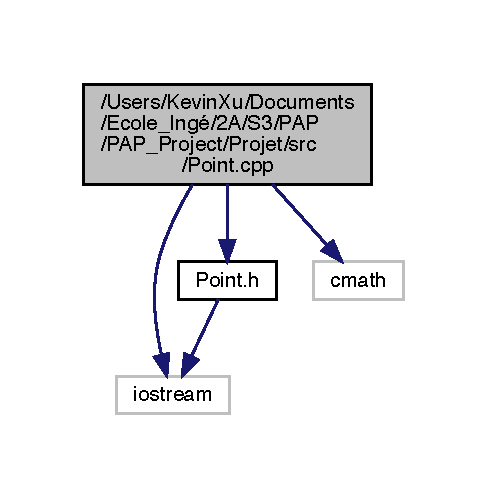
\includegraphics[width=234pt]{_point_8cpp__incl}
\end{center}
\end{figure}
\subsection*{Functions}
\begin{DoxyCompactItemize}
\item 
std\+::ostream \& \mbox{\hyperlink{_point_8cpp_aab579574359f43459927c5c2e52eed12}{operator$<$$<$}} (std\+::ostream \&out, const \mbox{\hyperlink{class_point}{Point}} \&P)
\begin{DoxyCompactList}\small\item\em Overload of the operator $<$$<$. \end{DoxyCompactList}\end{DoxyCompactItemize}


\subsection{Detailed Description}
Class \mbox{\hyperlink{class_point}{Point}} Implementation. 

\begin{DoxyAuthor}{Author}
Kevin XU \& Ziheng LI 
\end{DoxyAuthor}
\begin{DoxyDate}{Date}
30 Novembre 2018 
\end{DoxyDate}


\subsection{Function Documentation}
\mbox{\Hypertarget{_point_8cpp_aab579574359f43459927c5c2e52eed12}\label{_point_8cpp_aab579574359f43459927c5c2e52eed12}} 
\index{Point.\+cpp@{Point.\+cpp}!operator$<$$<$@{operator$<$$<$}}
\index{operator$<$$<$@{operator$<$$<$}!Point.\+cpp@{Point.\+cpp}}
\subsubsection{\texorpdfstring{operator$<$$<$()}{operator<<()}}
{\footnotesize\ttfamily std\+::ostream\& operator$<$$<$ (\begin{DoxyParamCaption}\item[{std\+::ostream \&}]{out,  }\item[{const \mbox{\hyperlink{class_point}{Point}} \&}]{P }\end{DoxyParamCaption})}



Overload of the operator $<$$<$. 


\begin{DoxyParams}{Parameters}
{\em out} & the output stream \\
\hline
{\em P} & \\
\hline
\end{DoxyParams}
\begin{DoxyReturn}{Returns}
out 
\end{DoxyReturn}

\begin{DoxyCode}
61                                                             \{
62     out << \textcolor{stringliteral}{"("} << P.\mbox{\hyperlink{class_point_ac9d5859db121c7d1b89ca89266dca0a3}{getX}}() << \textcolor{stringliteral}{", "} << P.\mbox{\hyperlink{class_point_a86d10ff46e08462c45b15a8c7ef62d61}{getY}}() << \textcolor{stringliteral}{")"};
63     \textcolor{keywordflow}{return} out;
64 \}
\end{DoxyCode}

\hypertarget{_point_8h}{}\section{/\+Users/\+Kevin\+Xu/\+Documents/\+Ecole\+\_\+\+Ingé/2\+A/\+S3/\+P\+A\+P/\+P\+A\+P\+\_\+\+Project/\+Projet/src/\+Point.h File Reference}
\label{_point_8h}\index{/\+Users/\+Kevin\+Xu/\+Documents/\+Ecole\+\_\+\+Ingé/2\+A/\+S3/\+P\+A\+P/\+P\+A\+P\+\_\+\+Project/\+Projet/src/\+Point.\+h@{/\+Users/\+Kevin\+Xu/\+Documents/\+Ecole\+\_\+\+Ingé/2\+A/\+S3/\+P\+A\+P/\+P\+A\+P\+\_\+\+Project/\+Projet/src/\+Point.\+h}}


Class \mbox{\hyperlink{class_point}{Point}}.  


{\ttfamily \#include $<$iostream$>$}\newline
Include dependency graph for Point.\+h\+:\nopagebreak
\begin{figure}[H]
\begin{center}
\leavevmode
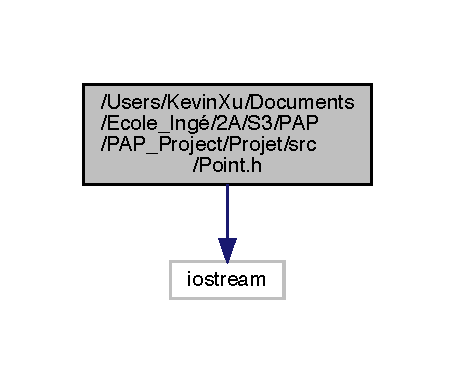
\includegraphics[width=218pt]{_point_8h__incl}
\end{center}
\end{figure}
This graph shows which files directly or indirectly include this file\+:
\nopagebreak
\begin{figure}[H]
\begin{center}
\leavevmode
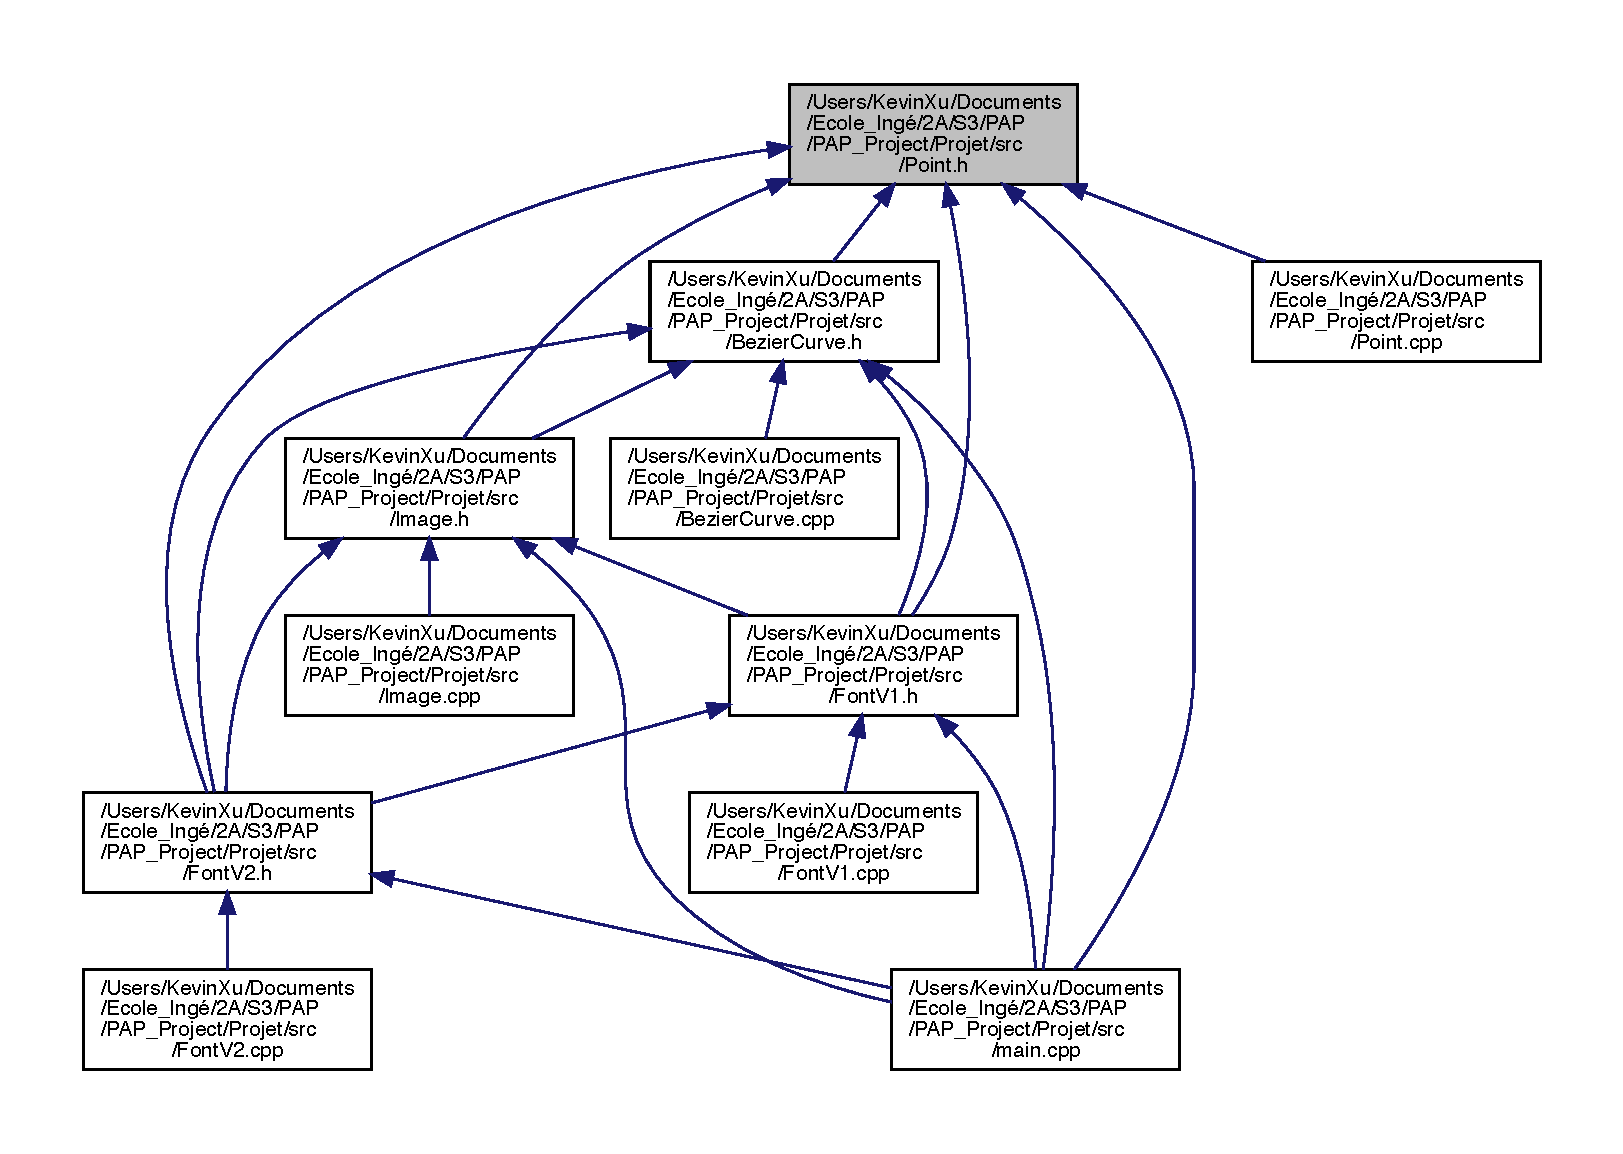
\includegraphics[width=350pt]{_point_8h__dep__incl}
\end{center}
\end{figure}
\subsection*{Classes}
\begin{DoxyCompactItemize}
\item 
class \mbox{\hyperlink{class_point}{Point}}
\end{DoxyCompactItemize}
\subsection*{Functions}
\begin{DoxyCompactItemize}
\item 
std\+::ostream \& \mbox{\hyperlink{_point_8h_aab579574359f43459927c5c2e52eed12}{operator$<$$<$}} (std\+::ostream \&out, const \mbox{\hyperlink{class_point}{Point}} \&P)
\begin{DoxyCompactList}\small\item\em Overload of the operator $<$$<$. \end{DoxyCompactList}\end{DoxyCompactItemize}


\subsection{Detailed Description}
Class \mbox{\hyperlink{class_point}{Point}}. 

\begin{DoxyAuthor}{Author}
Kevin XU \& Ziheng LI 
\end{DoxyAuthor}
\begin{DoxyDate}{Date}
30 Novembre 2018 
\end{DoxyDate}


\subsection{Function Documentation}
\mbox{\Hypertarget{_point_8h_aab579574359f43459927c5c2e52eed12}\label{_point_8h_aab579574359f43459927c5c2e52eed12}} 
\index{Point.\+h@{Point.\+h}!operator$<$$<$@{operator$<$$<$}}
\index{operator$<$$<$@{operator$<$$<$}!Point.\+h@{Point.\+h}}
\subsubsection{\texorpdfstring{operator$<$$<$()}{operator<<()}}
{\footnotesize\ttfamily std\+::ostream\& operator$<$$<$ (\begin{DoxyParamCaption}\item[{std\+::ostream \&}]{out,  }\item[{const \mbox{\hyperlink{class_point}{Point}} \&}]{P }\end{DoxyParamCaption})}



Overload of the operator $<$$<$. 


\begin{DoxyParams}{Parameters}
{\em out} & the output stream \\
\hline
{\em P} & \\
\hline
\end{DoxyParams}
\begin{DoxyReturn}{Returns}
out 
\end{DoxyReturn}

\begin{DoxyCode}
61                                                             \{
62     out << \textcolor{stringliteral}{"("} << P.\mbox{\hyperlink{class_point_ac9d5859db121c7d1b89ca89266dca0a3}{getX}}() << \textcolor{stringliteral}{", "} << P.\mbox{\hyperlink{class_point_a86d10ff46e08462c45b15a8c7ef62d61}{getY}}() << \textcolor{stringliteral}{")"};
63     \textcolor{keywordflow}{return} out;
64 \}
\end{DoxyCode}

%--- End generated contents ---

% Index
\backmatter
\newpage
\phantomsection
\clearemptydoublepage
\addcontentsline{toc}{chapter}{Index}
\printindex

\end{document}
